\documentclass[a4paper]{jreport}
\newcommand{\version}{5.0.1}

\title{{\vspace{2cm}{\Large Version \version} }}
\author{\Large Team SCALE\\ UGC working group}
\date{\today}


\usepackage[dvipdfmx]{graphicx, color}
\usepackage[dvipdfmx]{hyperref}
\usepackage{amsmath}
\usepackage{ascmac}
\usepackage{alltt}
\usepackage[round]{natbib}
\usepackage{tabularx}
\usepackage{color}
\usepackage{colortbl}
\usepackage{fancybox}
\usepackage{url}
\usepackage{pxjahyper}
\hypersetup{% options for hyperref
 bookmarksopen=true,
 bookmarksnumbered=true,
 colorlinks=true,
 linkcolor=red,
 citecolor=cyan,
 urlcolor=cyan,
}

%\setlength{\textwidth}{42zw}
%\setlength{\textheight}{40\baselineskip}
\usepackage[top=30mm,bottom=35mm,left=30mm,right=30mm]{geometry}
\usepackage{wallpaper}
%\renewcommand{\thefootnote}{\fnsymbol{footnote}}
\renewcommand{\thefootnote}{*\arabic{footnote})}

\newcommand{\namelist}[1]{{\color{magenta}\texttt{[\detokenize{#1}]}}}
\newcommand{\nmitem}[1]{{\color{magenta}\texttt{(\detokenize{#1})}}}
\newcommand{\XDIR}{X方向}
\newcommand{\YDIR}{Y方向}
\newcommand{\ZDIR}{Z方向}
%%%%
%%%% for chapter 5
\newcommand{\SecBasicDomainSetting}{{対象計算領域の設定}}
\newcommand{\SubsecRelationOfResoGridProcess}{{計算領域と解像度、格子点数、MPIプロセスの関係}}
\newcommand{\SubsecDomainSetting}{{計算領域の設定}}
\newcommand{\SubsecMPIProcess}{{MPIプロセス数}}
\newcommand{\SubsecGridNumSettng}{{水平・鉛直格子数の設定}}
\newcommand{\SubsecGridIntvSettng}{{水平・鉛直格子間隔の設定}}
\newcommand{\SecBasicBufferSetting}{{緩和領域の設定}}
\newcommand{\SecBasicTopoSetting}{{地形の設定}}
\newcommand{\SecBasicIntegrationSetting}{{積分時間と積分時間間隔の設定}}
\newcommand{\SecBasicOutputSetting}{{出力変数の追加・変更方法}}
\newcommand{\SecBasicDynamicsSetting}{{力学スキームの設定}}
\newcommand{\SubsecDynsolverSetting}{{数値解法の設定}}
\newcommand{\SubsecDynSchemeSetting}{{時間・空間差分スキームの設定}}
\newcommand{\SecBasicPhysicsSetting}{{物理スキームの設定}}
\newcommand{\SubsecMicrophysicsSetting}{{雲微物理スキームの設定}}
\newcommand{\SubsecTurbulenceSetting}{{乱流スキームの設定}}
\newcommand{\SubsecRadiationSetting}{{放射スキームの設定}}
\newcommand{\SubsecSurfaceSetting}{{地表面(大気下端境界)の設定}}
\newcommand{\SubsecOceanSetting}{{海洋モデルの設定}}
\newcommand{\SubsecLandSetting}{{陸面モデルの設定}}
\newcommand{\SubsecUrbanSetting}{{都市モデル(大気-都市面フラックス)の設定}}

%%%%
%%%% for chapter 6
\newcommand{\SecAdvanceMapprojectionSetting}{{地図投影法と計算領域の位置の設定}}
\newcommand{\SecAdvanceInputDataSetting}{{様々な初期値・境界値データを使用する}}
\newcommand{\SecAdvanceRestart}{{リスタート計算の方法}}



\begin{document}
\CenterWallPaper{1.0}{figure/title_wallpaper.eps}
\maketitle
\ClearWallPaper
\ULCornerWallPaper{.1}{figure/scale_logo_final_ULWB.eps}
\tableofcontents

\chapter{概要} \label{chap:overview}

%==============================================================%

本書は初めて領域気象気候モデル {\scalerm}
を利用する人に向けた解説書である。
気象気候ライブラリー{\scalelib}  version \version に対応した説明を記載する。
\scalelib の現バージョンには、領域モデル\scalerm と全球モデル\scalegm が含まれる。
本版では、\scalerm の使い方についてのみ詳しく述べる。
\scalegm については、次版で詳しく記載される予定である。
%\scalerm の使い方を通して、\scalelib を他のモデルからの呼び出す方法を
%習得することも可能です。

本書の構成は次の通りです。
第\ref{part:overview}部では SCALE の概要、
第\ref{part:install}部では必要な環境とインストール方法について説明する。
続いて、第\ref{chap:tutorial_ideal}章では理想実験、第\ref{chap:tutorial_real}章では現実大気実験を例にして、\scalerm の基本的な操作方法を説明する。
これらの章はひと繋がりのチュートリアルとなっており、
\scalerm を初めて使うユーザは一通り通読することを推奨する。
第\ref{part:basic_usel}部と第\ref{part:advance_use}部では、
モデルの設定の変更方法を記載し、また利用できるデータ形式やツールを説明する。
これらの各章は基本的にその中で閉じているので、辞書として用いることができる。

%%%
本書中の不明点やお気づきの点がございましたら、SCALE user's メーリングリスト\\
 \verb|scale-users@ml.riken.jp|までご連絡ください。



\section{\scalelib とは?} \label{subsec:scale_feature}
%--------------------------------------------------------------%

{\scalelib} (Scalable Computing for Advanced Library and Environment)は、
気候研究や天気予報を容易に様々な計算機上で行うためのソフトウェア・ライブラリである。
本ライブラリは、前処理からシミュレーション、後処理、解析に至るまで全ての過程を網羅し、
下記に挙げる長所を持つ。
\begin{itemize}
\item \scalelib は、「BSD-2ライセンス」のもとオープンソースソフトウェア
として提供している。
商用、非商用に関わらず自由な利用、改変、再配布が可能である。
\item \scalelib には、{\scalerm} (SCALE-Regional Model)
%SCALE-GM(SCALE-Global Model)
という領域モデルが含まれる。
\item \scalelib には、次節で説明するように様々なスキームが用意されている。
ユーザーが行いたい実験に合わせて適宜選択できる。
\item \scalelib では、\scalerm だけでなく他の数値モデルでも呼び出せる
物理過程のフレームワークを提供している。
\end{itemize}

ライセンスの詳細は、トップディレクトリ直下の\texttt{scale-\version/LICENSE}のファイルに記述されている。
\scalelib の使用前に一読されたい。
また、\scalelib のWebページ(\url{http://scale.aics.riken.jp/})にもソフトウェアの説明が記載されているので必要に応じて参照されたい。

本節では、\scalelib の思想や実際のモデルとの関係について説明する。
\scalerm の実行とは直接的には関係しないため、必要なければ読み飛ばしても構わない。

\Item{\scalelib のライブラリとモデルの関係について}

\begin{figure}[htb]
\begin{center}
  \includegraphics[width=0.9\hsize]{./figure/library_jp.eps}\\
  \caption{\scalelib のねらい}
  \label{fig:scale}
\end{center}
\end{figure}

\scalelib は幾つかの外部共同研究者と共に理化学研究所(RIKEN)で開発され、
その改良と拡張が継続的に行われている。
図 \ref{fig:scale}に\scalelib の思想の概念図を示す。
この図に示されるように、\scalelib は様々な問題に対応することを目指している。
\scalelib は、小型PCクラスターから次世代のスーパーコンピュータに至るまで様々な計算環境で広く用いられる事を念頭に開発されている。
この目的のため、気候・気象科学を専門とする科学者と計算機科学を専門とする科学者が
共同で開発している。

\scalerm は \scalelib ライブラリを大いに利用した数値モデルの一つであり、
図\ref{fig:scale-rm}に示すように \scalelib のパッケージに含まれる。
\scalelib は、並列プロセスの管理、ファイルの入出力、プロセス間の通信、格子情報の設定を行う。
また、\scalelib は、大気の流れのソルバ(力学コア)や雲微物理や大気放射等の物理過程も提供する。
その一方で、\scalerm は\scalelib が提供する機能を組み合わせることで構築されている。
\scalerm 自体は、大気の状態の入力データを予報変数として読み込んで保持し、
\scalelib の各コンポーネントを適宜呼び出すことで時間発展を計算する。
ユーザは行いたい実験に応じて、各コンポーネントのスキームを選択できる。

\begin{figure}[hbt]
\begin{center}
  \includegraphics[width=0.9\hsize]{./figure/scale_jp.eps}\\
  \caption{{\scalelib}ライブラリと{\scalerm}(モデル)の関係}
  \label{fig:scale-rm}
\end{center}
\end{figure}



\section{\scalerm の構成}  \label{subsec:sturcture_scale_rm}
%--------------------------------------------------------------%
\scalelib に含まれる全てのコンポーネント中の全てのスキームを、
\scalerm において利用できる。
コンポーネントは3つの部分(フレームワーク、力学コア、物理過程)に分類される。
以下に、\scalerm の現版に実装済みである、様々なスキームを含むコンポーネントを列挙する%
\footnote{
モデルの構成や離散化法の詳細は、
\citet{scale_2015}、\citet{satoy_2015b}、
\citet{nishizawa_2015}を参照されたい。
}。
\\

{\bf フレームワーク}
\begin{itemize}
 \item 実距離に基づいた3次元カーテシアン格子系
 \item MPI通信を用いた2次元領域分割
 \item 各種地図投影法
 \item 領域ネスティングシステム(1 way:親領域$\to$子領域へデータ転送)
   \begin{itemize}
    \item オンライン・ネスティング: 複数ドメインの計算を同時に実行
    \item オフライン・ネスティング:外側ドメインの計算終了後に、その結果を用いて内側ドメインの計算を実行
   \end{itemize}
 \item 複数事例一括実行システム(バルクジョブシステム)
 \item CF 規約\footnote{\url{http://cfconventions.org/}}に基づく \netcdf ファイル I/O
   \begin{itemize}
   \item {\netcdf}3 または {\netcdf}4 形式を選択
   \end{itemize}
 \item 理想実験のための初期値データ生成
 \item 外部データから標高・土地利用区分データを作成
 \item 外部データから初期値・境界値データを作成
   \begin{itemize}
    \item
      WRF-ARW\footnote{\url{http://www.wrf-model.org/}}、
%      NICAM\footnote{\url{http://nicam.jp/}}、
      \grads \footnote{\url{http://cola.gmu.edu/grads/}}形式での入力に対応
   \end{itemize}
\end{itemize}

{\bf 力学コア}
\begin{itemize}
 \item 支配方程式系: 3次元完全圧縮非静力学方程式系
 \item 空間離散化: 有限体積法
    \begin{itemize}
      \item 2次, 4次, 6次中央差分
      \item 3次, 5次風上差分
    \end{itemize}
 \item 時間離散化: 「完全陽解法」または「水平陽解法-鉛直陰解法」から選択
    \begin{itemize}
      \item Heun型3次ルンゲ・クッタスキーム
      \item \citet{Wicker_2002}の3段ルンゲ・クッタスキーム
      \item 4次ルンゲ・クッタスキーム
    \end{itemize}
 \item 非負保証:
    \begin{itemize}
      \item フラックス修正法 \citep[Flux Corrected Transport, FCT; ][]{zalesak_1979}
      \item \citet{Koren_1993}フィルター  (3次風上差分スキーム使用時のみ)
    \end{itemize}
 \item 数値フィルタ: 4次超粘性・拡散
 \item 地形: 地形に沿った座標系を用いて表現
\end{itemize}

{\bf 物理過程}
\begin{itemize}
 \item 乱流過程: 以下から選択可能
   \begin{itemize}
    \item \citet{smagorinsky_1963} \& \citet{lilly_1962}型のサブグリッドスケール乱流モデル (\citet{Brown_etal_1994}と\citet{Scotti_1993}による補正)
    \item \citet{Deardorff_1980} サブグリッドスケール乱流モデル
    \item \citet{my_1982,nakanishi_2004}によるlevel 2.5境界層乱流パラメタリゼーション
   \end{itemize}
 \item 雲微物理: 以下から選択可能
   \begin{itemize}
    \item \citet{kessler_1969}による3-class 1モーメントバルクモデル
    \item \citet{tomita_2008}による6-class 1モーメントバルクモデル
    \item \citet{sn_2014}による6-class 2モーメントバルクモデル
    \item \citet{suzuki_etal_2010}によるビン法モデル
   \end{itemize}
 \item 放射過程: \citet{sekiguchi_2008}による相関k分布法ブロードバンド大気放射伝達モデル
 \item 地表面モデル
  \begin{itemize}
   \item 陸面モデル: 熱拡散・バケツモデル
   \item 海洋モデル: 以下から選択可能
   \begin{itemize}
     \item 初期値固定
     \item 外部データ入力
     \item スラブモデル
   \end{itemize}
   \item 都市モデル: \citet{kusaka_2001}による単層キャノピーモデル
   \item バルク交換係数(陸面および海面): 以下から選択可能
   \begin{itemize}
     \item \citet{beljaars_1991,wilson_2001}による普遍関数によるバルク法
     \item \citet{uno_1995}によるLouis 型バルク法
   \end{itemize}
  \end{itemize}
\end{itemize}


This document assumes an execution in the shell ``bash'' on some Unix system.
If your environment is different, replace the commands
by the relevant commands suitable for your environment.
Unless there is a particular remark, this documentation obeys the following notation:

The command-line symbol for execution is expressed by \verb|$| or \verb|#|.
The difference between the two notations is
in the permission levels of program execution, as shown below:
\begin{verbatim}
 #        <- command by root permission
 $        <- command by user permission
\end{verbatim}

A description enclosed in a rectangle expresses a message generated by the command line, as shown below.
\msgbox{
 -- -- -- -- command-line message\\
 -- -- -- -- -- -- -- -- command-line message\\
 -- -- -- -- -- -- -- -- -- -- -- -- command-line message\\
}

On the other hand, a description enclosed in a rounded rectangle shows a part of configuration file including namelists, which can be edited as needed.
\editbox{
 -- -- -- -- description in a file\\
 -- -- -- -- -- -- -- -- description in a file\\
 -- -- -- -- -- -- -- -- -- -- -- -- description in a file\\
}

In this documentation, the FORTRAN namelist and its items are denoted by
\namelist{namelist} and \nmitem{item_of_namelist}, respectively.



\chapter{インストール} \label{chap:install}
\section{Installation of SCALE-LES}
%####################################################################################

本章では,日本域を対象とした現実大気再現実験のチュートリアルを通して,
SCALE-LESモデルを実行する一連の作業を説明する.
SCALEライブラリのインストールに必要な環境、ライブラリのインストール方法については,
\ref{sec:req_env}節とAppendix \ref{sec:env_setting}を参照して
事前にインストールしておく必要がある.
\ref{sec:source_code}以降のチュートリアルは,それらのライブラリ環境が
インストールされていることを想定して進める.


\subsection{Required Environment}
\label{sec:req_env}
%====================================================================================

\begin{itemize}
  \item {\bf 計算機環境} : Unix互換OS (Mac OS Xを含む)が動作する環境.
        マルチコアCPU環境以上を推奨する.
        実験サイズによるが4GB以上のメモリがインストールされているマシン環境が好ましい.
  \item {\bf OS} : Linux OS(Fedora, CentOS, SUSE等),Mac OS X.ここではLinux (CentOS6)を使用して説明する.
  \item {\bf コンパイラ} : Fortran 2003をサポートするC,Fortranコンパイラを必要とする.
        GNU 4.6.x以上,Intel compiler 2012以上を推奨する.ここでは,gcc/gfortranを使用して説明する.
  \item {\bf MPIライブラリ} : MPICH2, OpenMPI, Intel MPI等をサポートする.ここではopenMPIを使用して説明する.
  \item {\bf netcdf3 もしくは HDF5/netcdf4} : gzip, szipをサポートするHDF5,
        およびそのHDF5をサポートするnetcdf4を必要とする.
        ただし,netcdf3の環境下ではscaleライブラリが提供する全ての機能をサポートできない可能性がある.
  \item {\bf 描画環境(非必須)} : Dennou Club提供のRuby DCL/GPhysに含まれるgpviewがあると
        計算結果を簡単にチェックできる.チュートリアルではgpviewを使用する.
        それ以外に,netcdfからGrADS用にフォーマットを変換するためのpostprocess(\verb|netcdf2grads_h|)も用意している.
  \item SCALEは演算性能評価のためにPAPIライブラリを使用が可能.
        PAPIライブラリがインストールされている環境下では,
        以下で説明するconfigureファイルの編集によってPAPIを適用することができます.
\end{itemize}


\subsection{Building the source code} \label{sec:source_code}
%====================================================================================

\subsubsection{ソースコードの入手}
%-----------------------------------------------------------------------------------

安定版ソースコードは,\url{http://scale.aics.riken.jp/ja/download/index.html}
よりダウンロードすることができる.
ソースコードのtarballファイルを展開すると
\begin{verbatim}
  scale/
\end{verbatim}
というディレクトリができる.

現実大気実験のシミュレーションを行う場合,SCALE本体に加えて境界値データが必要になる.
本チュートリアル用の気象場のデータ,日本領域の地形・土地利用のデータを\\
 \url{http://scale.aics.riken.jp/download/tutorial_data.tar.gz}\\
より入手し,チュートリアルの入力ファイル用ディレクトリ
\begin{verbatim}
  scale/scale-les/test/tutorial/data/
\end{verbatim}
の下に展開しておく.

以降の説明で\verb|${TOPDIR}|は,\verb|scale/scale-les/test/tutorial/|がある絶対PATHを指す.

\begin{verbatim}
  ${TOPDIR}/data/tutorial_data/input_atom/    <- 気象場データ
  ${TOPDIR}/data/tutorial_data/input_topo/    <- 地形データ
  ${TOPDIR}/data/tutorial_data/input_landuse/ <- 土地利用データ
\end{verbatim}
\verb|tutorial_data/|には,本チュートリアルに必要な最低限のデータのみが納めされているため,
その他の設定で実験を行う場合には別途,気象場,地形,および土地利用データが必要となる.


\subsubsection{configure ファイルと環境変数の設定}
%-----------------------------------------------------------------------------------

\verb|scale/sysdep/|内にいくつかのコンフィグファイル(\verb|Makedef.***|)が準備されている.
これらの中から自分の環境にあったものを設定する.
ここでは,OSはLinux,コンパイラはgcc/gfortran,およびopenMPIを使用するため,
\verb|"Makedef.Linux64-gnu-ompi"|が対応するファイルとなる.
自分の環境に合うものがなければ既存ファイルをベースにして作成する.

常にこのコンフィグファイルをしようするために、
\verb|Makedef.***|の\verb|"***"|の部分を、\verb|SCALE_SYS|という環境変数として設定し、
\verb|.bashrc|などのファイルに記述しておくと便利である.
さらに、SCALEをコンパイルするのに必要な外部ライブラリについても
下記のようにPATHを設定する.
ここでは,Appendix \ref{sec:env_setting}に従ったとして,
HDF5,netcdf4ともに\verb|/usr|の下にインストールされている場合の例を示す.

\begin{verbatim}
 $ export SCALE_SYS="Linux64-gnu-ompi"
 $ export HDF5="/usr"
 $ export NETCDF4="/usr"
\end{verbatim}


\subsubsection{コンパイル}
%-----------------------------------------------------------------------------------

下記のディレクトリに移動して,makeコマンドによってコンパイルを行う.
\begin{verbatim}
 $ cd ${TOPDIR}/bin
 $ make -j 4
\end{verbatim}
\verb|make|のあとの \verb|"-j 4"| は,並列コンパイルを指示するオプションで,
4並列コンパイルを行うことを指示している.
コンパイルを実行する環境によっては並列数を増やすこともできる.
このmakeによってSCALEライブラリ,およびSCALE-LESモデルのコンパイルが行われ,
結果として
\begin{verbatim}
 scale-les  scale-les_init  scale-les_pp
\end{verbatim}
の3つの実行ファイルが生成されていればコンパイルは成功である.\\


{\bf 注意点}
\begin{itemize}
\item SCALEライブラリは,scaleのTOPディレクトリ直下の
 \verb|scale/scalelib/|というディレクトリ内でコンパイルとアーカイブが行われ,
 \verb|".lib"|という名前の隠しディレクトリとして
 \verb|bin/|ディレクトリ内へコピーされている.
\item Debugモードでコンパイルしたい場合や,
 コンパイルオプションを変更したい場合は,
 \verb|Makedef.***|のファイルを編集してください.
\item 開発版ソースコードをコンパイルしている場合,
 一部のコンパイラバージョンにおいてコンパイルが正常に終了しないケースがあります.そのような場合はぜひSCALE開発チームまでご報告ください.
\end{itemize}


%####################################################################################



\chapter{チュートリアル: 理想実験} \label{chap:tutorial_ideal}
%%%%%%%%%%%%%%%%%%%%%%%%%%%%%%%%%%%%%%%%%%%%%%%%%%%%%%%%%%%%%%%%%%%%%
%  File 31_ideal_exp.tex
%%%%%%%%%%%%%%%%%%%%%%%%%%%%%%%%%%%%%%%%%%%%%%%%%%%%%%%%%%%%%%%%%%%%%
xo
\section{概要}

本章では、SCALEを使った理想実験の実行方法を説明する。
第\ref{sec:install}章で実行したSCALEのコンパイルが
正常に完了しているかどうかのチェックも含めてぜひ実施してもらいたい。


\subsection{チュートリアル実行のための推奨環境}
\label{sec:assumed_env}

本章のチュートリアルの説明は、下記の環境を前提として記述している。
コンパイラ、ライブラリについては、適宜、使用環境に合わせて読み替えること。

\begin{itemize}
 \item {\bf CPU} : 物理コアが2コア以上 %[Intel Core i5 2410M 2.3GHz 2コア/4スレッド] %、第\ref{chap:tutorial_real}章は4コアを搭載
 \item {\bf Memory} : 512MB以上 %[DDR3-1333 4GB]     %、第\ref{chap:tutorial_real}章は2GB
 \item {\bf OS} : Linux OS x86-64  %[CentOS 6.6、CentOS 7.1、openSUSE 13.2のいずれか]
 \item {\bf コンパイラ} : GNU コンパイラ(gcc/gfortran)
 \item {\bf MPIライブラリ} : openMPI(リポジトリ経由でのインストール)
\end{itemize}

本章では、SCALEのコンパイルが正常に終了し、
すでに下記のファイルが生成されているものとして説明を行う。
\begin{alltt} 
  scale-{\version}/scale-rm/test/tutorial/bin/scale-rm
  scale-{\version}/scale-rm/test/tutorial/bin/scale-rm_init
  scale-{\version}/scale-rm/util/netcdf2grads_h/net2g
\end{alltt}
これらに加えて、本章のチュートリアルでは、
描画ツールとしてGrADSを使用する。
gpviewは、結果の確認用に利用することができる。
GrADSおよびgpview(GPhys)との詳細やインストール方法については、
付録 \ref{sec:env_vis_tools}節を参照のこと。


\subsection{実験設定}
%====================================================================================

実験設定として、積雲対流の理想実験を例にあげる。
この実験では、積乱雲が発生するときの
典型的な大気の鉛直プロファイルと対流圏下層に初期擾乱を与え、
積乱雲が発達する様子を準2次元モデルで実験する内容となっている。
実験設定は表\ref{tab:setting_ideal}に示す通りである。

\begin{table}[htb]
\begin{center}
\caption{チュートリアル理想実験の実験設定}
\begin{tabularx}{150mm}{|l|X|X|} \hline
 \rowcolor[gray]{0.9} 項目 & 設定内容 & 備考 \\ \hline
 水平格子間隔 & 東西:500 m、南北:1000 m & 東西-鉛直の面を切り取った準2次元実験である \\ \hline
 水平格子点数 & 東西:40、南北:2\footnotemark &  \\ \hline
 鉛直層数     & 97層(トップ:20 km)& 下層ほど細かい層間隔をとったストレッチ設定である \\ \hline
 側面境界条件 & 周期境界 & 東西、南北とも \\ \hline
 積分時間間隔 & 5 sec      & 雲微物理スキームは10 sec毎 \\ \hline
 積分期間     & 3,600 sec  & 720 steps \\ \hline
 データ出力間隔 & 300 sec  &  \\ \hline
 物理スキーム & 雲微物理モデルのみ使用 &
 6-class single moment bulk model \citep{tomita_2008} \\ \hline
 初期鉛直プロファイル & GCSS Case1 squall-line \citep{Redelsperger2000}&
 風のプロファイルは、\citet{Ooyama_2001}に基づいた鉛直シアを与える \\ \hline
 初期擾乱 & ウォームバブル & 水平半径4 km、
 鉛直半径3 kmの大きさを持つ最大プラス3Kの強度のウォームバブルを置く\\ \hline
\end{tabularx}
\label{tab:setting_ideal}
\end{center}
\end{table}
\footnotetext{現在は2次元実験を行うための枠組みは用意されていないが、{\YDIR}に同じ値をもつ初期値を与える事で2次元実験に相当する実験を行うことが可能である。この場合、ハロの格子数と同じ数の格子数を{\YDIR}に設定する必要がある。ハロの必要格子数については\ref{subsec:atmos_dyn_scheme}参照。}









\section{実行方法} \label{sec:ideal_exp_run}
%====================================================================================

実験の実行は、前準備、初期値作成、シミュレーション実行、後処理、そして描画の順番で作業を進める。

\Item{実験設定}
%====================================================================================

チュートリアル理想実験として、積雲対流の理想実験を用意している。
この実験では、積乱雲が発生するときの
典型的な大気の鉛直プロファイルと対流圏下層に初期擾乱を与え、
積乱雲が発達する様子を準2次元モデルで実験する内容となっている。
実験設定を表\ref{tab:setting_ideal}に示す。

\begin{table}[htb]
\begin{minipage}{150mm}
\begin{center}
\caption{本章での理想実験の実験設定}
\begin{tabularx}{150mm}{|l|X|X|} \hline
 \rowcolor[gray]{0.9} 項目 & 設定内容 & 備考 \\ \hline
 MPIプロセス数 & 東西:2、南北:1 & 計2プロセスでの並列計算を行う \\ \hline
 水平格子間隔 & 東西:500 m、南北:1000 m & 東西-鉛直の面を切り取った準2次元実験である \\ \hline
 水平格子点数 & 東西:40、南北:2\footnote{現在は2次元実験を行うための枠組みは用意されていないが、{\YDIR}に同じ値をもつ初期値を与える事で2次元実験に相当する実験を行うことが可能である。この場合、ハロの格子数と同じ数の格子数を{\YDIR}に設定する必要がある。ハロの必要格子数については\ref{subsec:atmos_dyn_scheme}参照。} &  \\ \hline
 鉛直層数     & 97層(トップ:20 km)& 下層ほど細かい層厚をもつストレッチ設定である \\ \hline
 側面境界条件 & 周期境界 & 東西、南北境界とも \\ \hline
 積分時間間隔 & 5 sec      & 雲微物理スキームは10 sec毎 \\ \hline
 積分期間     & 3,600 sec  & 720 steps \\ \hline
 データ出力間隔 & 300 sec  &  \\ \hline
 物理スキーム & 雲微物理モデルのみ使用 &
 6-class single moment bulk model \citep{tomita_2008} \\ \hline
 初期鉛直プロファイル & GCSS Case1 squall-line \citep{Redelsperger2000}&
 風のプロファイルは、\citet{Ooyama_2001}に基づいた鉛直シアを与える \\ \hline
 初期擾乱 & ウォームバブル & 水平半径4 km、
 鉛直半径3 kmの大きさを持つ最大プラス3Kの強度のウォームバブルを置く\\ \hline
\end{tabularx}
\label{tab:setting_ideal}
\end{center}
%\footnotetext{現在は2次元実験を行うための枠組みは用意されていないが、{\YDIR}に同じ値をもつ初期値を与える事で2次元実験に相当する実験を行うことが可能である。この場合、ハロの格子数と同じ数の格子数を{\YDIR}に設定する必要がある。ハロの必要格子数については\ref{subsec:atmos_dyn_scheme}参照。}
\end{minipage}
\end{table}


\subsection{前準備} \label{subsec:ideal_exp_prepare}
%------------------------------------------------------
チュートリアル理想実験は、\verb|scale-rm/test/tutorial/ideal|の
ディレクトリにて実行する。
このディレクトリに移動し、
scale-{\version}/binにある実行バイナリへの静的リンクを張る。
\begin{alltt}
  $ cd scale-rm/test/tutorial/ideal
  $ ln -s ../../../../bin/scale-rm      ./
  $ ln -s ../../../../bin/scale-rm_init ./
\end{alltt}
``\verb|scale-rm|''はモデル本体、
``\verb|scale-rm_init|''は初期値・境界値作成ツールである。

\subsection{初期値作成} \label{subsec:ideal_exp_init}
%------------------------------------------------------
初期値の作成は、\verb|scale-rm_init|に
設定ファイルを与えて実行する。
\verb|init_R20kmDX500m.conf| には、
表\ref{tab:setting_ideal} に対応した実験設定が書き込まれている。
この設定ファイルを\verb|scale-rm_init|に与えて実行することで、
設定ファイルの指示に従って大気の成層構造を計算し、初期擾乱が設定される。


SCALEの基本的な実行コマンドは下記のとおりである。
\begin{alltt}
  $ mpirun  -n  [プロセス数]  [実行バイナリ名]  [設定ファイル]
\end{alltt}
[プロセス数]の部分にはMPI並列で使用したいプロセス数を記述する。
[実行バイナリ]には、\verb|scale-rm|や\verb|scale-rm_init|が入る。
そして、実験設定を記述した設定ファイルを[設定ファイル]の部分に指定する。
%
例えば、
\verb|init_R20kmDX500m.conf|は2-MPI並列(2つのMPIプロセス)を使って計算するように指定されている。
\verb|scale-rm_init|を実行するコマンドは次のように記述する。
\begin{alltt}
  $ mpirun  -n  2  ./scale-rm_init  init_R20kmDX500m.conf
\end{alltt}
%
\noindent 実行が成功した場合、コマンドラインのメッセージは
下記のように表示される。\\

\noindent {\small {\gt
\fbox{
\begin{tabularx}{140mm}{l}
 *** Start Launch System for SCALE-RM\\
 *** Execute preprocess? :  T\\
 *** Execute model?      :  F\\
 *** a single comunicator\\
 *** a single comunicator\\
 *** End   Launch System for SCALE-RM\\
\end{tabularx}
}}}\\


\noindent この実行によって、
\begin{alltt}
  init_LOG.pe000000
  init_00000101-000000.000.pe000000.nc
  init_00000101-000000.000.pe000001.nc
\end{alltt}
の3つのファイルが、現在のディレクトリ下に作成される。
ログファイル(\verb|init_LOG.pe000000|)には、
コマンドラインには表示されない詳しい実行ログが記録されている。
ファイル名の\verb|pe|の後の数字は、MPIのプロセス番号を示している。
例では2つのMPIプロセスを利用しているが、
デフォルト設定では0番目のプロセス(マスターランク)のログファイルだけが出力される。
%すべてのプロセスの実行ログを出力するよう設定を変更することも出来る。
実行が正常に終了している場合、このLOGファイルの最後に\\

\noindent {\small {\gt
\fbox{
\begin{tabularx}{140mm}{l}
 ++++++ Finalize MPI...\\
 ++++++ MPI is peacefully finalized\\
\end{tabularx}
}}}\\

\noindent と記述される。\\
\verb|init_00000101-000000.000.pe000000.nc|と\verb|init_00000101-000000.000.pe000001.nc|の
2つのファイルは初期値ファイルであり、それぞれおおよそ100KBのファイルサイズになる。
計算領域全体を2つのMPIプロセスで分割し担当するため、
2つのファイルが生成される。
もし、4-MPI並列で実行すれば、4つの初期値ファイルが生成される。
これらのファイル名の末尾が``.nc''で終わるファイルは
NetCDF形式のファイルであり、
GPhys/Ruby-DCLやncviewといったツールで直接読むことができる。



\subsection{モデル本体の実行} \label{subsec:ideal_exp_run}
%------------------------------------------------------
プロセス並列数は、初期値作成のときと同じ数を指定する。
設定ファイルには \verb|run_R20kmDX500m.conf| を指定する。
\begin{alltt}
  $ mpirun  -n  2  ./scale-rm  run_R20kmDX500m.conf
\end{alltt}

本書の必要要件にあった計算機であれば、2分程度で計算が終わる。
\noindent この実行によって、
\begin{alltt}
  LOG.pe000000
  history.pe000000.nc
  history.pe000001.nc
\end{alltt}
の3つのファイルが、現在のディレクトリ下に作成されているはずである。
\verb|LOG.pe000000| には、
コマンドラインには表示されない詳しい実行ログが記録されている。
実行が正常に終了している場合、このLOGファイルの最後に\\

\noindent {\small {\gt
\fbox{
\begin{tabularx}{140mm}{l}
 ++++++ Finalize MPI...\\
 ++++++ MPI is peacefully finalized\\
\end{tabularx}
}}}\\

\noindent と記述される。
\verb|history.pe000000.nc| と \verb|history.pe000001.nc|
の2つのファイルが計算結果が記録されたhistoryファイルであり、それぞれおおよそ1.4MBのファイルサイズになる。
2-MPI並列で実行したため、2つのファイルが生成されており、ファイル形式はNetCDFである。
%``monitor.pe000000''は、計算中にモニタリングしている
%物理変数の時間変化を記録したテキストファイルである。


\section{Post-processing and drawing} \label{sec:ideal_exp_net2g}
%------------------------------------------------------
In this section, we explain post-processing and the method of drawing the calculation result.  In the tutorial, the distributed files in \netcdf format are merged into one file and converted into simple binary form ({\grads} form) that can be directly accessed. The binary form makes it easy for users to analyze the result. Link to the post-processing tool \verb|net2g| compiled  in Section \ref{sec:source_net2g}:
\begin{verbatim}
  $ ln -s ../../../util/netcdf2grads_h/net2g  ./
\end{verbatim}

The method of execution of \verb|net2g| is the same as that of \scalerm, i.e.,
\begin{verbatim}
 $ mpirun -n [the number of the processes] ./net2g [the configuration file] 
\end{verbatim}
The configuration file \verb|net2g.conf| is intended for special uses of \verb|net2g|.
Give this configuration file to \verb|net2g| and execute it as follows:
\begin{verbatim}
  $ mpirun  -n  2  ./net2g  net2g.conf
\end{verbatim}
If there is no error message and the following message is displayed to the standard output,
the conversion is completed without problem:
\msgbox{
\verb|+++ MPI COMM: Corrective Finalize| \\
}

The execution of net2g should be handled,
so that the number of MPI processes is identical to, or a divisor of, that used for the run of \scalerm. The following six files are generated under the same directory by this execution:
\begin{alltt}
  QHYD_d01z-3d.ctl
  QHYD_d01z-3d.grd
  U_d01z-3d.ctl
  U_d01z-3d.grd
  W_d01z-3d.ctl
  W_d01z-3d.grd
\end{alltt}
The ``grd'' files are the converted files in the simple binary form of direct access
({\grads} form) obtained by merging the divided files,
whereas the ``ctl'' files are used to render them readable by \grads.
%In this case, these files contain U (horizontally eastern wind), W (vertical wind), and QHYD (mass concentration of total hydrometeors).

To confirm whether the calculation is satisfactory,
draw a figure using \grads script \verb|checkfig_ideal.gs|.
Note that the grammar depends on the version of \grads.
If a warning appears, the \grads script should be rewritten appropriately:
\begin{verbatim}
  $ grads -blc checkfig_ideal.gs
\end{verbatim}
If it is successfully completed, the following files are generated:

\begin{verbatim}
   ideal_QHYD.png
   ideal_W.png
\end{verbatim}
The same figures as Fig. \ref{fig_ideal} can be found in the simulation,
and post-processing is successfully concluded.

\begin{figure}[t]
\begin{center}
  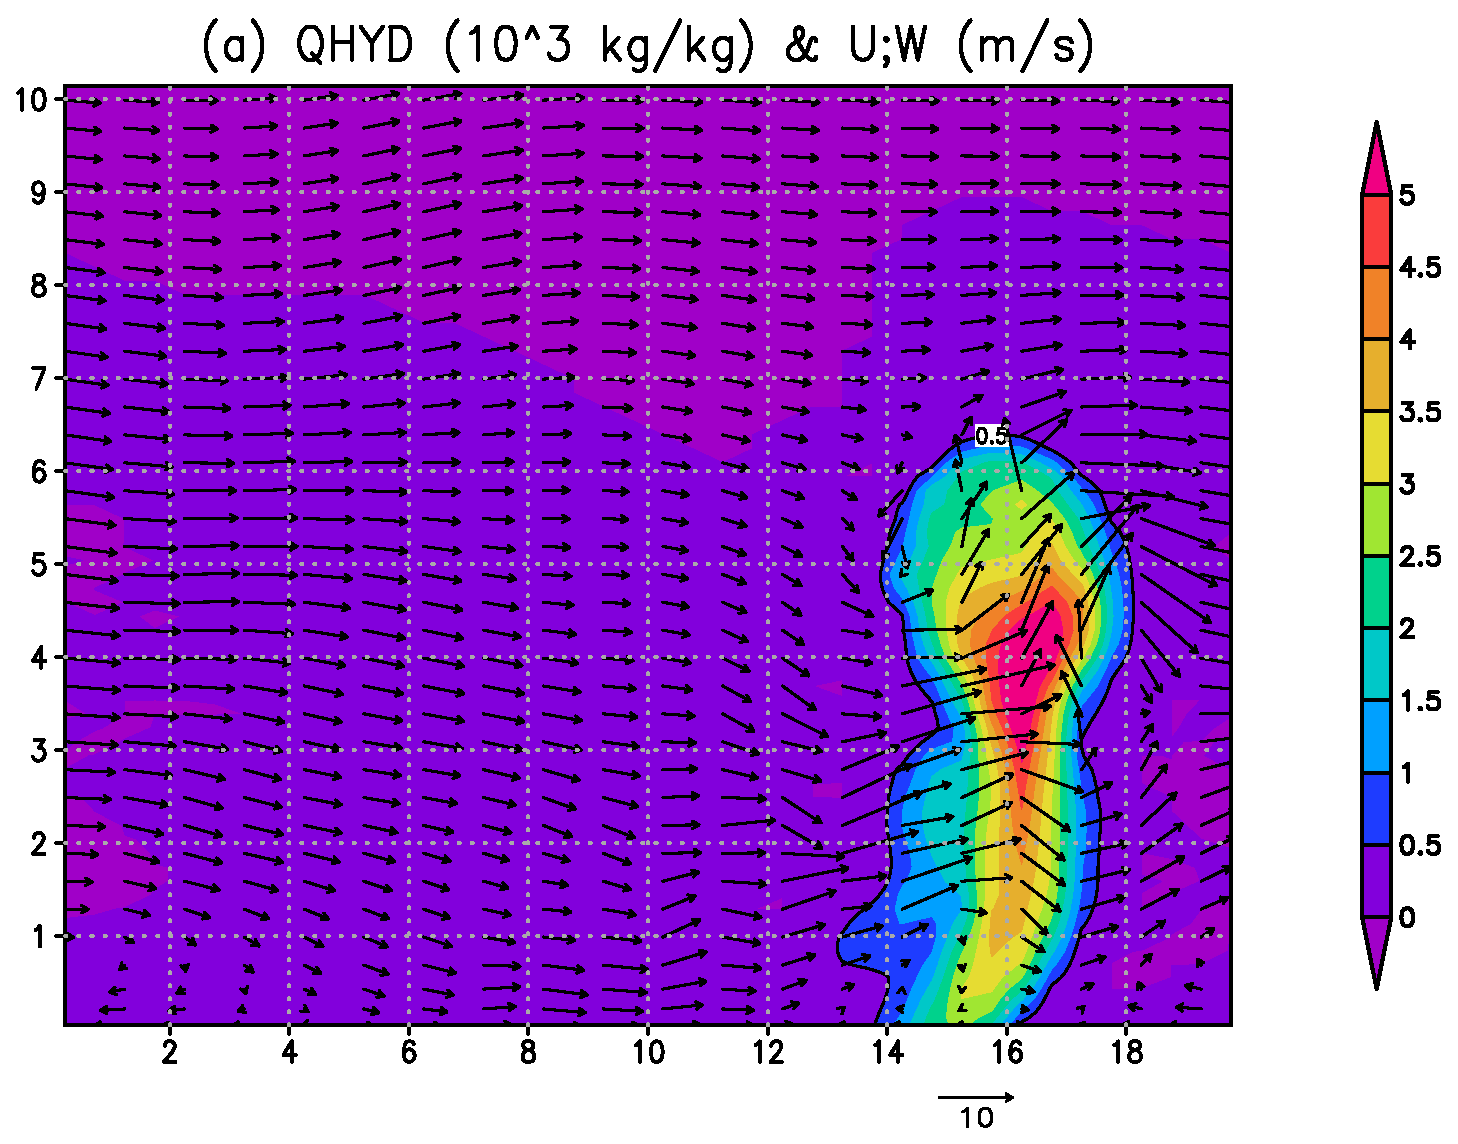
\includegraphics[width=0.7\hsize]{./figure/ideal_qhyd.eps}\\
  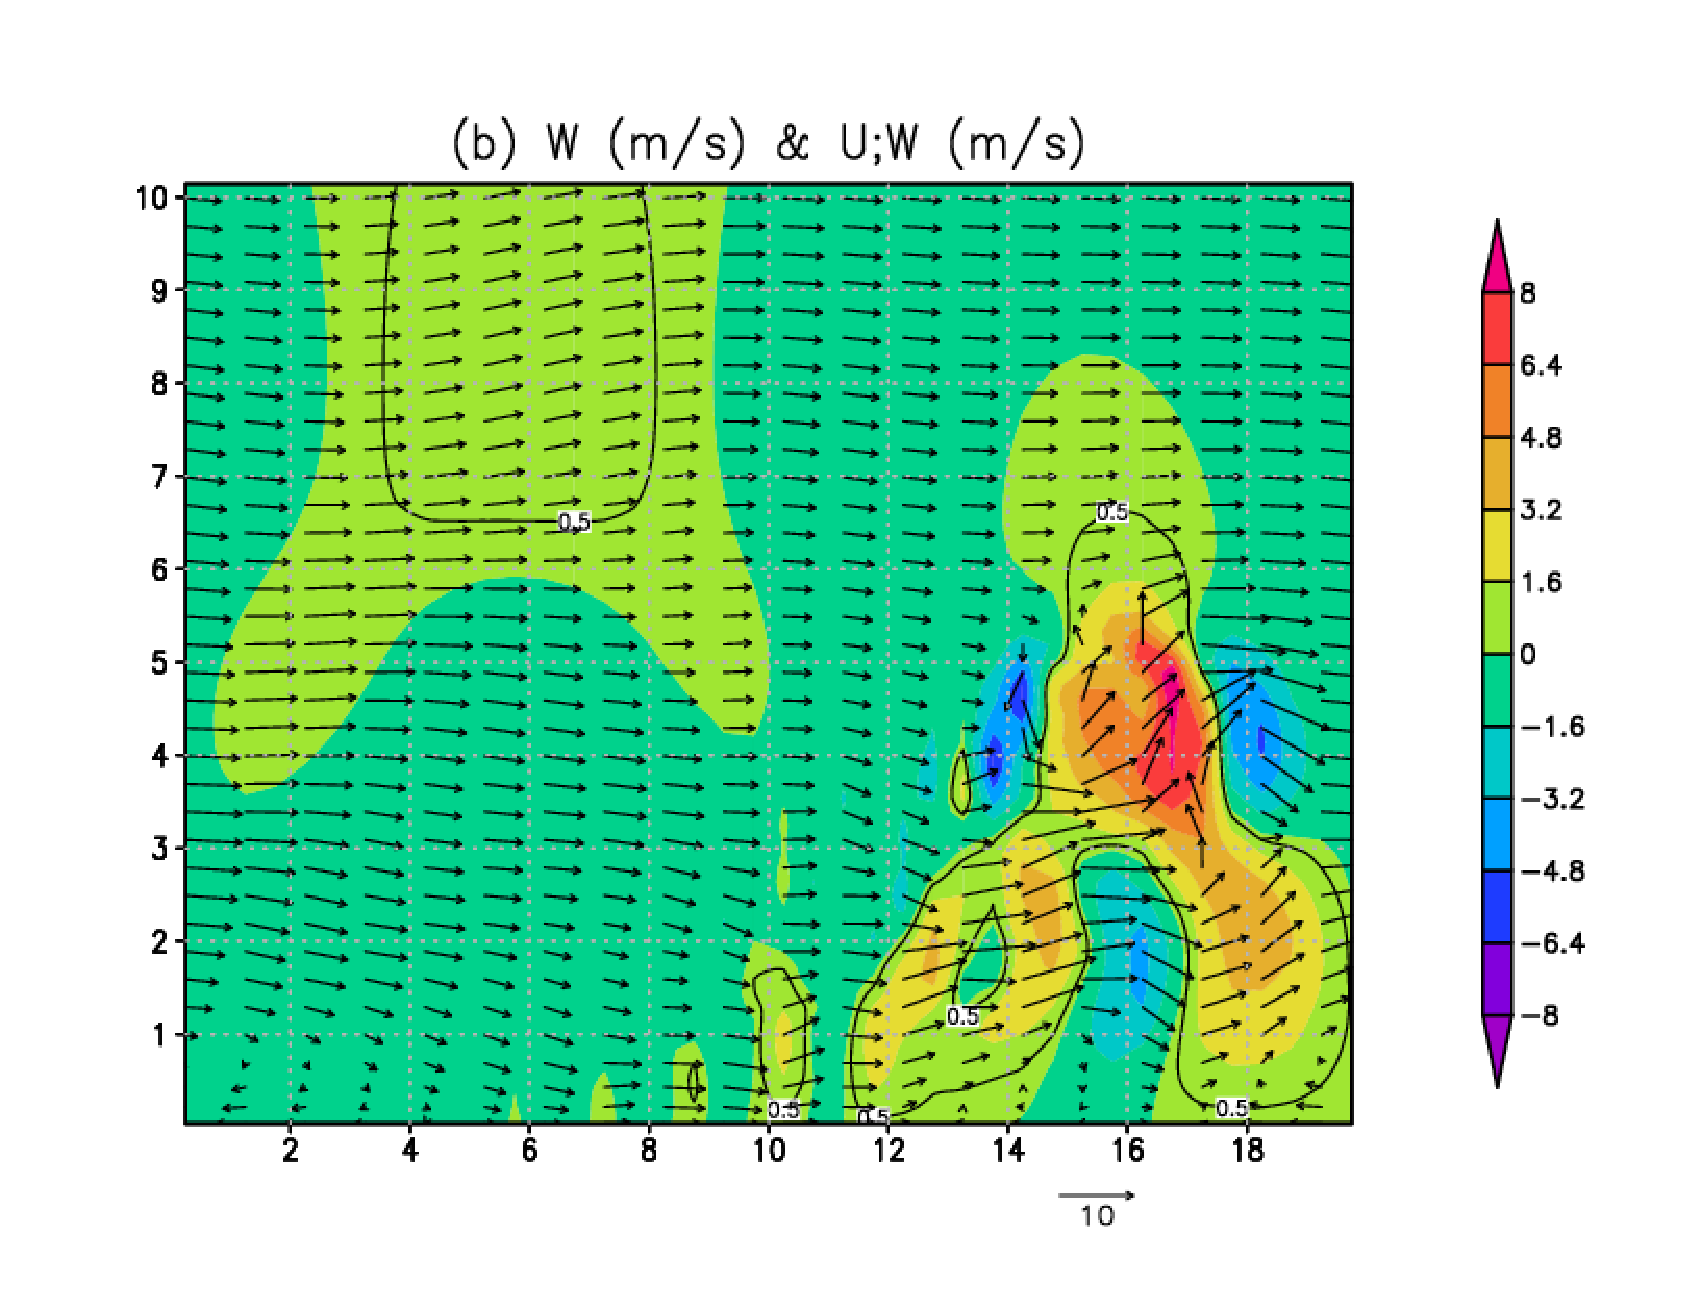
\includegraphics[width=0.7\hsize]{./figure/ideal_W.eps}\\
  \caption{The horizontal-vertical cross-section at Y=750m after t=1200 s (20 minutes later);
            The color indicates (a) the mass concentration of the hydrometeor and (b) vertical velocity. The vector indicates flow in both of figures.}
  \label{fig_ideal}
\end{center}
\end{figure}

To convert the result of the output into binary data for other variables,
add them to \nmitem{VNAME} in \namelist{VARI} in the configuration file \verb|net2g.conf|:
\editbox{
\verb|&VARI|\\
\verb| VNAME       = "U","W","QHYD"|\\
\verb|/|\\
}
To check the output variable in the history file, use \verb|ncdump| of {\netcdf}.
Refer to Section \ref{sec:net2g} for the detailed use of net2g. 


\section{Guideline for further study} \label{sec:ideal_exp_last}

In this chapter,
the method for the execution of \scalerm was explained by using a simple ideal experiment. We recommend studying methods of changing the model resolution, the calculation domain, and the number of MPI processes for further study.  With regard to the ideal experiment, several files of other configurations,  e.g., to increase resolution, the number of domains, and the physical scheme, are prepared in the directory ``sample'' under the same directory as was used in this experiment.  These configuration files are useful to change such configurations.  Moreover, various ideal experimental settings  have been prepared in the directory ``\verb|scale-rm/test/case|.'' For some ideal experiments,  it may be necessary to carry out the ``make'' command again in the same directory as in the configuration file  because some test cases need special source codes according to their experimental settings. The procedures for the generation of the initial conditions and those for simulation execution are the same as in the tutorial in this chapter.

It is important to study the method for the configuration of physical processes, such as cloud microphysics, radiation, and turbulence schemes. Methods to alter them in detail are described in Part \ref{part:basic_usel}.



\chapter{チュートリアル: 現実実験} \label{chap:tutorial_reall}
%-------------------------------------------------------%
\section{概要} \label{sec:tutrial_real_intro}
%-------------------------------------------------------%
本章では、チュートリアルとして準備した現実大気実験の基本的な実行手順を習得する。
現実大気実験は、次の流れ(図\ref{fig:howto}) に従って実行する。
\begin{enumerate}
\item  入力データの準備 (基本各自で準備。チュートリアルでは \verb|tools/| で行う。)
\item  \texttt{pp}      : 地形データの作成
\item  \texttt{init}    : 初期値・境界値データの作成
\item  \texttt{run}     : シミュレーションの実行
\item  \texttt{net2g}   : 出力データの\netcdf から\grads 形式への変換(オプション)
\end{enumerate}

\begin{figure}[b]
\begin{center}
  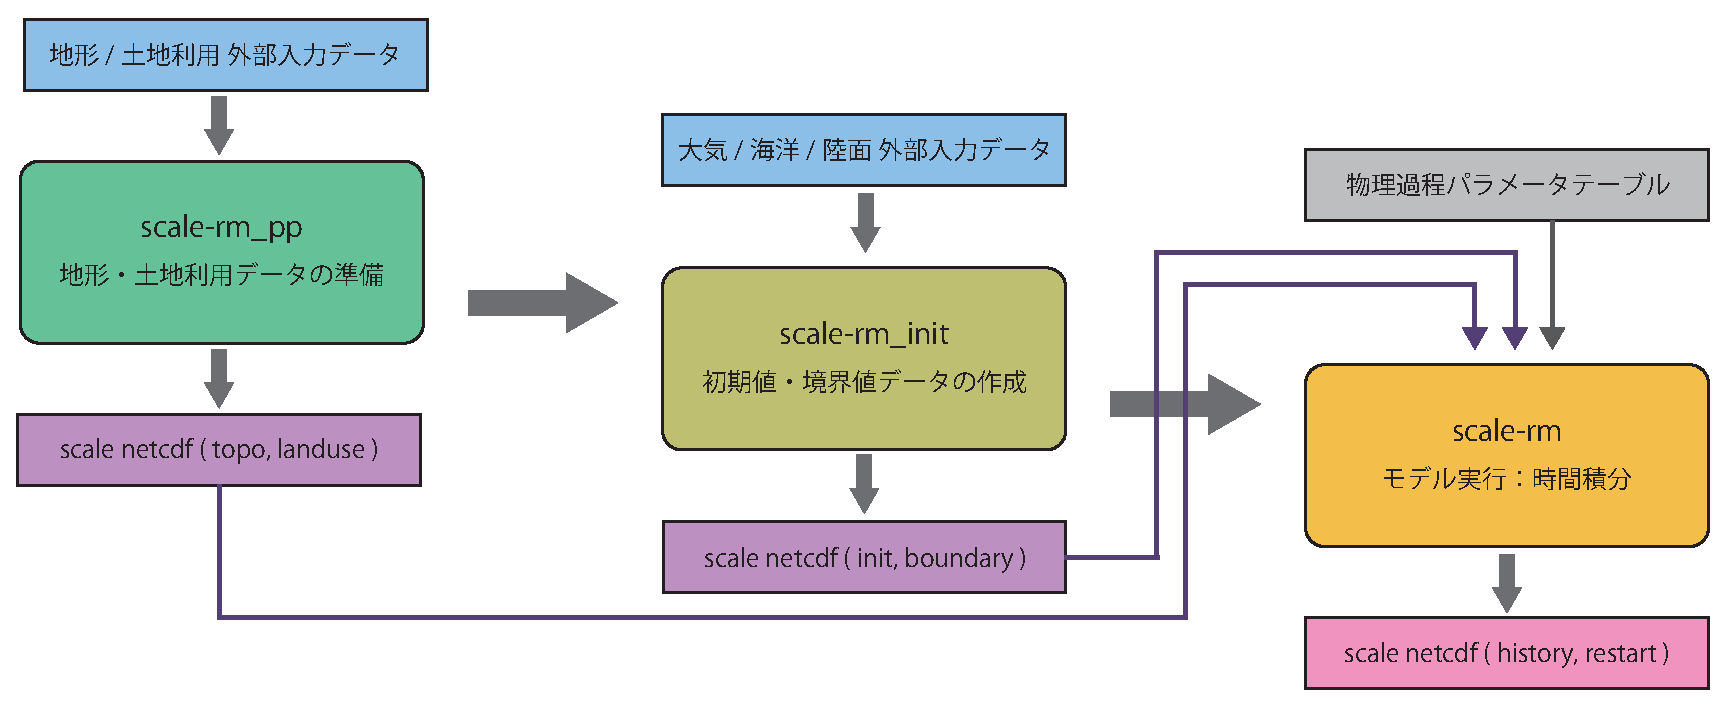
\includegraphics[width=0.9\hsize]{./figure/real_procedure.eps}\\
  \caption{\scalerm モデルの実行過程}
  \label{fig:howto}
\end{center}
\end{figure}


これ以降の説明では、\texttt{scale-{\version}/scale-rm/test/tutorial/}の絶対パスを
\verb|${Tutorial_DIR}|と示すこととする。


チュートリアルの現実大気実験の計算領域(ドメイン)の設定は表\ref{tab:grids}のようになっている。
図 \ref{fig:tutrial_real_domain}に対象領域を示す。
このチュートリアルは、\scalerm の使い方を学ぶことが目的であり、
短い時間で実行可能な設定にしている。
領域モデルの実験設定として必ずしも適切な設定を選択しているとは限らないので
ご留意頂きたい
(例えば、20kmの水平解像度で積雲パラメタリゼーションなし)。
%本章のチュートリアルを比較的短時間で実行するには、下記の条件を満たす計算機環境が推奨される。
%\begin{itemize}
%\item CPU: 2コア以上の演算コアを持つCPU(4コア以上を推奨)
%\item Memory容量: 4GB以上をプログラムに割当可能(8GB以上を搭載した計算機を推奨)
%\item HDD空き容量: 7GB以上の空き容量
%\end{itemize}


\begin{table}[h]
\begin{center}
  \caption{実験設定の概略}
  \label{tab:grids}
  \begin{tabularx}{150mm}{|l|X|} \hline
    \rowcolor[gray]{0.9} 項目 & 設定 \\ \hline
    MPIプロセス分割 (東西 x 南北) & 2 x 2 (合計4プロセス) \\ \hline
    水平格子数 (東西 x 南北) & 90格子点 x 90格子点 \\ \hline
    鉛直層数                 & 36層                  \\ \hline
    水平格子間隔             & dx = dy = 20km       \\ \hline
    積分期間 & 2007年7月14日 18UTC~15日00UTC (6時間積分) \\ \hline
    時間ステップ間隔 & 90 sec (240 steps) \\ \hline
  \end{tabularx}
\end{center}
\end{table}

\begin{figure}[tb]
\begin{center}
  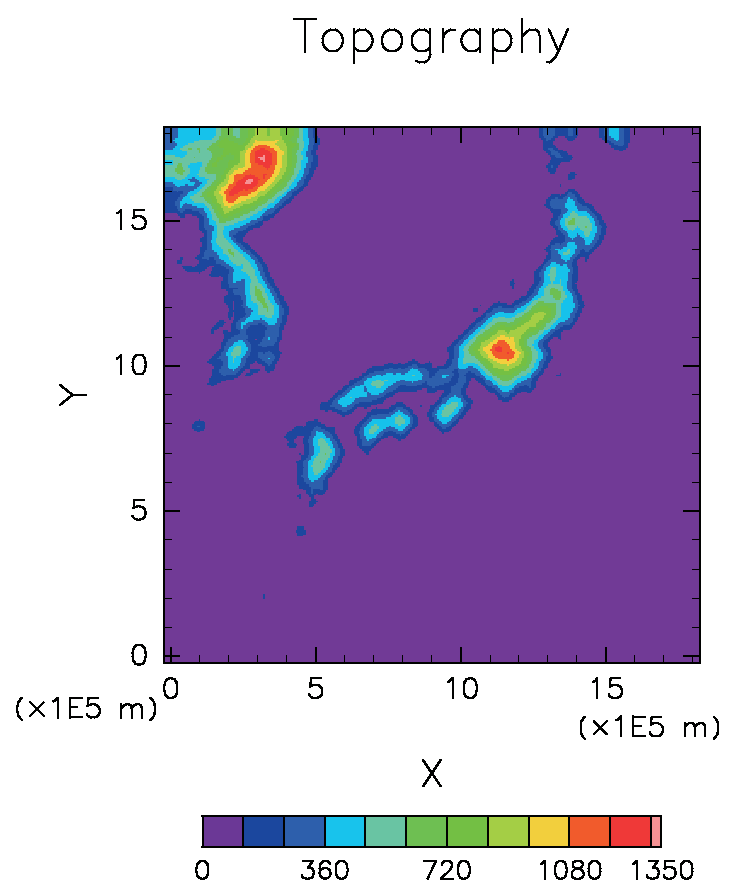
\includegraphics[width=1.0\hsize]{./figure/real_domain.eps}\\
  \caption{計算領域の地形と海陸分布.}
  \label{fig:tutrial_real_domain}
\end{center}
\end{figure}



%-------------------------------------------------------%
\section{境界データの準備}
\label{sec:tutrial_real_prep}
%-------------------------------------------------------%

現実大気実験のシミュレーションを行う場合、SCALE本体に加えて
境界値データが必要になる。境界値データとしては表\ref{tab:real_bnd}
が必要である。{\color{blue}青字}は必須の変数、その他は任意である。

\begin{table}[h]
\begin{center}
  \caption{現実大気実験に必要な初期値境界値データ}
  \label{tab:real_bnd}
  \begin{tabularx}{150mm}{llX} \hline
    \multicolumn{3}{l}{地形データ(SCALE-RMの地形を用意する)}\\ \hline
    & \multicolumn{2}{l}{\color{blue}{標高データ}}\\
    & \multicolumn{2}{l}{\color{blue}{土地利用データ}}\\ \hline
    \multicolumn{3}{l}{初期値境界値データ}\\ \hline
    &  \multicolumn{2}{l}{\color{blue}{親モデルの緯度・経度}}\\
    &  \multicolumn{2}{l}{(3次元大気データ)}\\
    & &  \multicolumn{1}{l}{\color{blue}{東西風速, 南北風速, 気温, 比湿(相対湿度), 気圧, ジオポテンシャル高度}} \\
    &  \multicolumn{2}{l}{(2次元大気データ)}\\
    & & 海面更正気圧, 地上気圧, 10m東西風速, 10m南北風速, 2m気温, 2m比湿(相対湿度) \\
    &  \multicolumn{2}{l}{(2次元陸面データ)}\\
    & &  \multicolumn{1}{l}{親モデルの海陸マップ}\\
    & &  \multicolumn{1}{l}{\color{blue}{地表面温度(Skin temp)}}\\
    & &  \multicolumn{1}{l}{{\color{blue}{親モデル土壌データの深さ情報, 土壌温度}}, 土壌水分(体積含水率 or 飽和度)}\\
    &  \multicolumn{2}{l}{(2次元海面データ)}\\
  & &  \multicolumn{1}{l}{\color{blue}{海面水温(Skin tempがある場合は省略可)}}\\ \hline
  \end{tabularx}
\end{center}
\end{table}


\subsubsection{地形データと土地利用データ}
標高データと土地利用データは実験設定に従って、
SCALEのそれぞれの格子点における地形、海陸分布、土地利用を
作成するために使用する。
ユーザーが全球の任意の地域を対象とした計算ができるよう、
フォーマット変換済みの
標高データ USGS(U.S. Geological Survey) のGTOPO30 と、
土地利用データ GLCCv2 を提供している。

\begin{enumerate}
\item データのダウンロード\\
SCALE用の地形・土地利用のデータを\\
 \url{http://scale.aics.riken.jp/download/scale_database.tar.gz}\\
より入手し、任意のディレクトリに展開しておく。
\begin{alltt}
  $ tar -zxvf scale_database.tar.gz
\end{alltt}
展開したディレクトリには、地形データと土地利用データが格納されている。
\begin{alltt}
  scale_database/topo/    <- 地形データ
  scale_database/landuse/ <- 土地利用データ
\end{alltt}

\item パスの設定\\
makeを使ったジョブスクリプトを使用する場合には、
展開先のディレクトリを \verb|SCALE_DB| という環境変数に設定しておくことが必須である
(以後、\verb|${SCALE_DB}|と表記)。
\begin{alltt}
  $ export SCALE_DB=${path_to_directory_of_scale_database}/scale_database
\end{alltt}
\end{enumerate}

\subsubsection{大気・陸面・海面水温データ}
\label{sec:tutrial_real_prep_fnl}
初期値境界値データは4-byte バイナリー(grads format)に変換すれば、
任意のデータを読み込むことが可能である。
チュートリアルではNCEP FNL(Final) Operational Global Analysis dataを使用する。
あらかじめ\verb|wgrib|をインストールしておく。
\footnote{\url{http://www.cpc.ncep.noaa.gov/products/wesley/wgrib.html}}
\begin{enumerate}
\item データのダウンロード\\
NCARのサイト
\url{http://rda.ucar.edu/datasets/ds083.2/}\\
から、2007年7月14日18時から一日分のgrib1フォーマットのデータ
\begin{alltt}
fnl_20070714_18_00.grib1
fnl_20070715_00_00.grib1
fnl_20070815_06_00.grib1
fnl_20070815_12_00.grib1
\end{alltt}
を\verb|${Tutorial_DIR}/real/tools/|の下にダウンロードする。
\item データフォーマットをgribからbinaryに変換\\
 SCALEは4byte バイナリー(grads format)の境界値データを読み込むことができる。\\
\verb|${Tutorial_DIR}/real/tools/| の中にある \verb|convert_grib2grads.sh|を実行。

\begin{alltt}
  $ sh convert_grib2grads.sh
\end{alltt}
成功すれば、下記のファイルが作成される。
\begin{alltt}
 $ ls -al FNL_output/*/*
FNL_output/200707/FNLatm_2007071418.grd
FNL_output/200707/FNLatm_2007071500.grd
FNL_output/200707/FNLatm_2007071506.grd
FNL_output/200707/FNLatm_2007071512.grd
FNL_output/200707/FNLland_2007071418.grd
FNL_output/200707/FNLland_2007071500.grd
FNL_output/200707/FNLland_2007071506.grd
FNL_output/200707/FNLland_2007071512.grd
FNL_output/200707/FNLsfc_2007071418.grd
FNL_output/200707/FNLsfc_2007071500.grd
FNL_output/200707/FNLsfc_2007071506.grd
FNL_output/200707/FNLsfc_2007071512.grd
\end{alltt}
\end{enumerate}


%-------------------------------------------------------%
\section{地形・土地利用データの作成:pp} \label{sec:tutrial_real_pp}
%-------------------------------------------------------%

ppディレクトリへ移動し、現実実験のための地形データ、土地利用データを作成する。
\begin{verbatim}
 $ cd ${Tutorial_DIR}/real/pp
\end{verbatim}
ppディレクトリの中には、\verb|pp.conf|という名前の
設定ファイルが準備されている。
ドメインの位置や格子点数など、実験設定に合わせて、
適宜\verb|pp.conf|を編集する必要があるが、
チュートリアルではすでに表\ref{tab:grids}の設定に
従って編集済みの\verb|pp.conf|が用意されているためそのまま利用する。
\verb|pp.conf|の設定の中で確認してほしい項目は、\namelist{PARAM_CONVERT}である。\\

\noindent {\gt
\ovalbox{
\begin{tabularx}{140mm}{l}
\verb|&PARAM_CONVERT| \\
\verb|  CONVERT_TOPO = .true.,| \\
\verb|  CONVERT_LANDUSE = .true.,| \\
\verb|/| \\
\end{tabularx}
}}\\

\noindent 上記のように\nmitem{CONVERT_TOPO}と\nmitem{CONVERT_LANDUSE}が
\verb|.true.|となっていることが、
それぞれ地形と土地利用の処理を行うことを意味している。
詳細なコンフィグファイルの内容については、
付録\ref{app:namelist}を参照されたい。

次に、コンパイル済みのバイナリと入力データを
pp実行ディレクトリへリンクする。
\begin{verbatim}
 $ ln -s ../../bin/scale-rm_pp ./
 $ ln -s ${SCALE_DB}/topo    ./
 $ ln -s ${SCALE_DB}/landuse ./
\end{verbatim}
今回は、表\ref{tab:grids}に示されているように。
4つのMPIプロセスを使用する設定なので次のように実行する。
\begin{verbatim}
 $ mpirun -n 4 ./scale-rm_pp pp.conf
\end{verbatim}
%本節使用した環境において、実行にはおおよそ15秒を要する。
ジョブが正常に終了すれば、\verb|topo_d01.pe######.nc|と\\
\verb|landuse_d01.pe######.nc|と
いうファイルがMPIプロセス数だけ、つまり4つずつ生成される(
\verb|######|にはMPIプロセスの番号が入る)。
それぞれ、各格子点における地形と土地利用の情報が入っている。
実行時のログは、\verb|pp_LOG_d01.pe000000|に出力されるので内容を確かめておくこと。


%% サポート外
%% \vspace{1cm}
%% \noindent {\Large\em OPTION} \hrulefill \\
%% gpviewがインストールされている場合、次のコマンドによって、
%% 作成された地形と土地利用データが正しく作成されているかどうか
%% 確認することが出来る.正しく作成されていれば,図 \ref{fig:tutrial_real_domain}と同様の図ができる.
%% \begin{verbatim}
%%   $ gpview topo_d01.pe00000*@TOPO --aspect=1 --nocont
%%   $ gpview landuse_d01.pe00000*@FRAC_LAND --aspect=1 --nocont
%% \end{verbatim}



%-------------------------------------------------------%
\section{初期値・境界値データの作成:init}
%-------------------------------------------------------%

init では、SCALE計算に必要な初期値・境界値データを作成する。
まず、initディレクトリへ移動する。
\begin{verbatim}
 $ cd ${Tutorial_DIR}/real/init
\end{verbatim}
ディレクトリの中には、\verb|init.conf|という名前の設定ファイルが準備されている。
\verb|pp.conf|と同様に、実験設定に合わせて、この\verb|init.conf|を書き換える必要があるが、
チュートリアル用の\verb|init.conf|ファイルは表\ref{tab:grids}の設定に
すでに合わせてある。
初期値・境界値データの作成には前節で作成した地形・土地利用データを利用する。
これは、\verb|init.conf|の中で、下記のように相対PATHを用いて参照するように設定されている。\\

\noindent {\gt
\ovalbox{
\begin{tabularx}{140mm}{l}
\verb|&PARAM_TOPO| \\
\verb|   TOPO_IN_BASENAME = "../pp/topo_d01",| \\
\verb|/| \\
 \\
\verb|&PARAM_LANDUSE| \\
\verb|   LANDUSE_IN_BASENAME  = "../pp/landuse_d01",| \\
\verb|/| \\
\end{tabularx}
}}\\

\noindent その他に\verb|init.conf|の設定の中で特に確認してほしい項目は、
\verb|PARAM_MKINIT_REAL|である。\\

\noindent {\gt
\ovalbox{
\begin{tabularx}{140mm}{l}
\verb|&PARAM_MKINIT_REAL| \\
\verb|   BASENAME_BOUNDARY    = "boundary_d01",|   {\small ← 境界値データの出力名} \\
\verb|   FILETYPE_ORG         = "GrADS",| \\
\verb|   NUMBER_OF_FILES      = 3,|                      {\small ← 読み込むファイルの数} \\
\verb|   BOUNDARY_UPDATE_DT   = 21600.D0,|           {\small ← 入力データの時間間隔} \\
\verb|   INTERP_SERC_DIV_NUM  = 20,|                   {\small ← 内挿計算用のチューニングパラメータ} \\
\verb|   PARENT_MP_TYPE       = 3,| \\
\verb|   USE_FILE_DENSITY     = .false.,|          {\small ← 親モデルの大気密度データを使うか} \\
\verb|   USE_FILE_LANDWATER   = .true.,|           {\small ← 親モデルの土壌水分データを使うか} \\
\verb|   INTRP_LAND_SFC_TEMP  = "mask",|           {\small ← 親モデルの欠測値処理方法} \\
\verb|   INTRP_LAND_TEMP      = "fill",| \\
\verb|   INTRP_LAND_WATER     = "fill",| \\
\verb|   INTRP_OCEAN_SFC_TEMP = "mask",| \\
\verb|   INTRP_OCEAN_TEMP     = "mask",| \\
\verb|/| \\
\end{tabularx}
}}\\

\noindent \verb|FILETYPE_ORG|は入力する気象場データのファイルフォーマットに
関するパラメータを設定しており、ここでは
grads形式のデータを読み込むことを指定している。
詳細な設定ファイルの内容については、付録\ref{app:namelist}を参照されたい。

次に、コンパイル済みのバイナリをinitディレクトリへリンクする。
\begin{verbatim}
  $ ln -s ../../bin/scale-rm_init ./
\end{verbatim}
\ref{sec:real_prep}節で作成した入力データに、
initディレクトリの中に準備されている\verb|"gradsinput-link_FNL.sh"|を用いてリンクをはる。
\begin{verbatim}
  $ sh gradsinput-link_FNL.sh
\end{verbatim}
下記のgrads形式のファイルにリンクが張れれば成功である。\\

\noindent {\gt
\fbox{
\begin{tabularx}{140mm}{l}
\verb|FNLatm_00000.grd -> ../tools/FNL_output/200707/FNLatm_2007071418.grd| \\
\verb|FNLatm_00001.grd -> ../tools/FNL_output/200707/FNLatm_2007071500.grd| \\
\verb|FNLatm_00002.grd -> ../tools/FNL_output/200707/FNLatm_2007071506.grd| \\
\verb|FNLatm_00003.grd -> ../tools/FNL_output/200707/FNLatm_2007071512.grd| \\
\verb|FNLland_00000.grd -> ../tools/FNL_output/200707/FNLland_2007071418.grd| \\
\verb|FNLland_00001.grd -> ../tools/FNL_output/200707/FNLland_2007071500.grd| \\
\verb|FNLland_00002.grd -> ../tools/FNL_output/200707/FNLland_2007071506.grd| \\
\verb|FNLland_00003.grd -> ../tools/FNL_output/200707/FNLland_2007071512.grd| \\
\verb|FNLsfc_00000.grd -> ../tools/FNL_output/200707/FNLsfc_2007071418.grd| \\
\verb|FNLsfc_00001.grd -> ../tools/FNL_output/200707/FNLsfc_2007071500.grd| \\
\verb|FNLsfc_00002.grd -> ../tools/FNL_output/200707/FNLsfc_2007071506.grd| \\
\verb|FNLsfc_00003.grd -> ../tools/FNL_output/200707/FNLsfc_2007071512.grd| \\
\end{tabularx}
}}\\






次に、陸面の変数を用意するのに必要なパラメータファイルにリンクをはる。
\begin{verbatim}
 $ ln -s ../../../data/land/* ./   <- 陸面スキーム用のパラメータファイル
\end{verbatim}
準備が整ったら、4つのMPIプロセスを使用してinitを実行する。
\begin{verbatim}
 $ mpirun -n 4 ./scale-rm_init init.conf
\end{verbatim}

正常にジョブが終了すると、
\begin{verbatim}
 $ ls
  boundary_d01.pe000000.nc
  boundary_d01.pe000001.nc
  boundary_d01.pe000002.nc
  boundary_d01.pe000003.nc
  init_d01_20070714-180000.000.pe000000.nc
  init_d01_20070714-180000.000.pe000001.nc
  init_d01_20070714-180000.000.pe000002.nc
  init_d01_20070714-180000.000.pe000003.nc
  init_LOG_d01.pe000000
\end{verbatim}
が作成される。
\verb|boundary_d01.pe######.nc|は境界値データ、
\verb|init_d01_20070714-180000.000.pe######.nc|は初期値データ、
\verb|init_LOG_d01.pe######|はログファイルである。
\verb|######|はMPIプロセス番号を表している。


%% サポート外
%% \vspace{1cm}
%% \noindent {\Large\em OPTION} \hrulefill \\
%% gpviewがインストールされている場合,作成された初期値と境界値が
%% 正しく作成されているかどうかを確認することが出来る。
%% 正しく作成されていれば、図 \ref{fig:init}と同じように描かれる。

%% \begin{verbatim}
%% $ gpvect --scalar --slice z=1500 --nocont --aspect=1 --range=0.002:0.016          \
%%          --xintv=10 --yintv=10 --unit_vect init_d01_20140810-000000.000.pe00*@QV      \
%%          init_d01_20140810-000000.000.pe00*@MOMX init_d01_20140810-000000.000.pe00*@MOMY
%% \end{verbatim}


%% \begin{figure}[h]
%% \begin{center}
%%   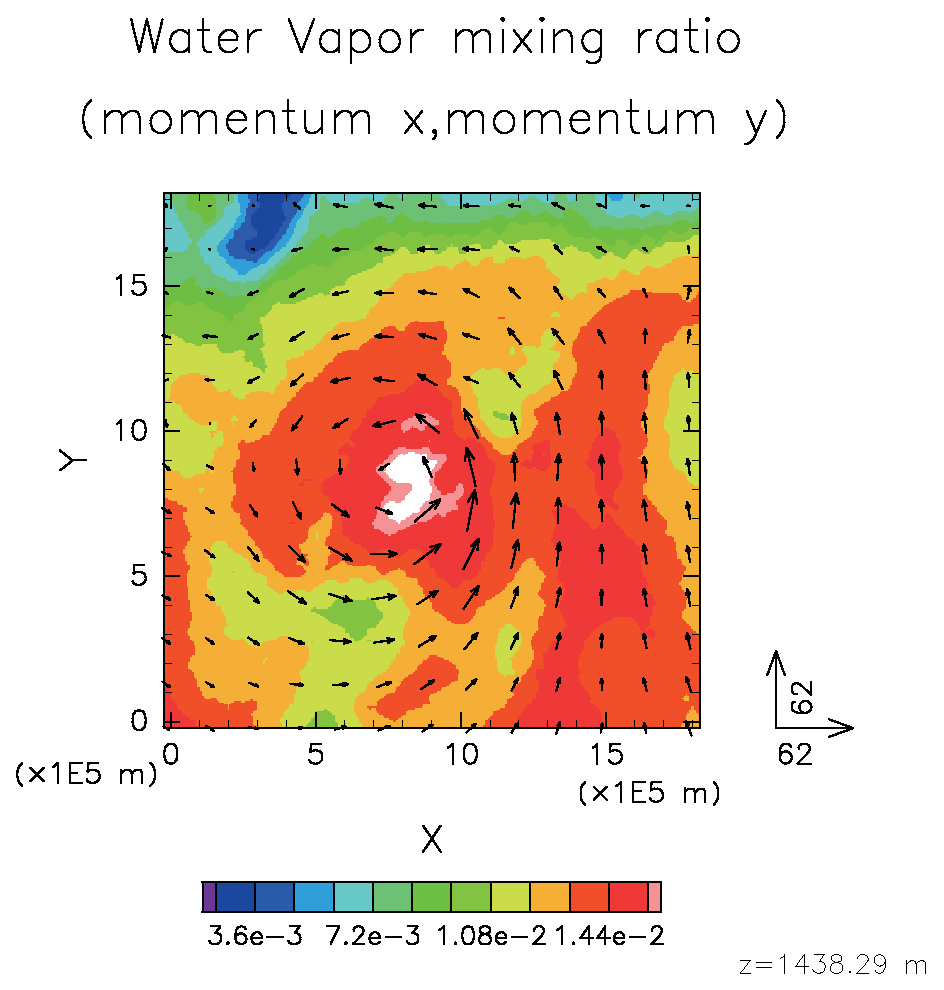
\includegraphics[width=0.7\hsize]{./figure/init_qv-momxy.eps}\\
%%   \caption{チュートリアル実験の高さ1500mにおける初期場の様子.カラーシェードは比湿,
%%            ベクトルは水平運動量フラックスを表している.}
%%   \label{fig:init}
%% \end{center}
%% \end{figure}


%-------------------------------------------------------%
\section{時間積分を行う:run}
\label{sec:tutrial_real_run}
%-------------------------------------------------------%
\subsubsection{run.confの準備}
runディレクトリへ移動する。
\begin{verbatim}
 $ cd ${Tutorial_DIR}/real/run
\end{verbatim}
%
runディレクトリの中には、\verb|run.conf|という名前の
設定ファイルが準備されており、
ドメインの位置や格子点数など、
チュートリアル用の設定(表\ref{tab:grids})に合わせて設定されている。\\

\noindent {\small {\gt
\ovalbox{
\begin{tabularx}{140mm}{l}
\verb|&PARAM_PRC| \\
\verb| PRC_NUM_X      = 2,| \\
\verb| PRC_NUM_Y      = 2,| \\
\verb| PRC_PERIODIC_X = .false.,| \\
\verb| PRC_PERIODIC_Y = .false.,| \\
\verb|/| \\
 \\
\verb|&PARAM_INDEX| \\
\verb| KMAX = 36,| \\
\verb| IMAX = 45,| \\
\verb| JMAX = 45,| \\
\verb|/| \\
\end{tabularx}
}}}\\


{\XDIR} 、{\YDIR}ともに2分割されており、
総計として4つのMPIプロセスを使用する設定となっている。
1つのMPIプロセスあたりの格子点数については、
\nmitem{IMAX = 45}、\nmitem{JMAX = 45}と指定されているため、
{\XDIR} 、{\YDIR}の総格子点数は、ともに$2 \times 45$ で90である。
計算ドメインの大きさは、
\namelist{PARAM_GRID}の\nmitem{DX}、\nmitem{DY}はともに20000 m(20 km)
と指定されているため、
90 個$\times$ 20 km より、1800 km $\times$ 1800 km の正方形の計算領域
が設定されていることがわかる。


モデル本体の実行には
事前に作成した地形・土地利用データや初期値・境界値データを利用する。
これらのファイルの指定は、
\verb|run.conf|の下記部分で設定する。\\

\noindent {\gt
\ovalbox{
\begin{tabularx}{140mm}{l}
\verb|&PARAM_TOPO| \\
\verb|   TOPO_IN_BASENAME = "../pp/topo_d01",| \\
\verb|/| \\
 \\
\verb|&PARAM_LANDUSE| \\
\verb|   LANDUSE_IN_BASENAME  = "../pp/landuse_d01",| \\
\verb|/| \\
 \\
\verb|&PARAM_RESTART| \\
\verb|   RESTART_OUTPUT      = .false.,| \\
\verb|   RESTART_IN_BASENAME = "../init/init_d01_20070714-180000.000",| \\
\verb|/| \\
 \\
\verb|&PARAM_ATMOS_BOUNDARY| \\
\verb|   ATMOS_BOUNDARY_TYPE        = "REAL",| \\
\verb|   ATMOS_BOUNDARY_IN_BASENAME = "../init/boundary_d01",| \\
\verb|   ATMOS_BOUNDARY_USE_VELZ    = .true.,| \\
\verb|   ATMOS_BOUNDARY_USE_QHYD    = .false.,| \\
\verb|   ATMOS_BOUNDARY_VALUE_VELZ  = 0.0D0,| \\
\verb|   ATMOS_BOUNDARY_UPDATE_DT   = 21600.0D0,| \\
\verb|/| \\
\end{tabularx}
}}\\


\verb|run.conf|の設定の中で時間積分に関する設定は、
\namelist{PARAM_TIME}の項目にある。\\

\noindent {\gt\small
\ovalbox{
\begin{tabularx}{150mm}{ll}
\verb|&PARAM_TIME| & \\
\verb| TIME_STARTDATE     = 2007, 7, 14, 0, 0, 0,| &← 時間積分を開始する時刻 \\
\verb| TIME_STARTMS       = 0.D0,| &\\
\verb| TIME_DURATION      = 6.0D0,| &← 積分期間 \\
\verb| TIME_DURATION_UNIT = "HOUR",| &← \verb|TIME_DURATION|の単位\\
\verb| TIME_DT            = 90.0D0,| &← トレーサー移流計算の時間ステップ\\
\verb| TIME_DT_UNIT       = "SEC",|  &← \verb|TIME_DT|の単位\\
\verb| TIME_DT_ATMOS_DYN  = 45.0D0,| &← トレーサー移流計算以外の力学過程の時間ステップ\\
\verb| TIME_DT_ATMOS_DYN_UNIT = "SEC",| &← \verb|TIME_DT_ATMOS_DYN|の単位\\
 \\
\verb| ~~中略~~| &\\
 \\
\verb|/| &\\
\end{tabularx}
}}\\

\noindent 初期時刻は、\nmitem{TIME_STARTDATE}においてUTCで指定する。
チュートリアルでは2007年7月14日18時UTCに設定している。
積分のための時間ステップは、上記の他、
それぞれの物理スキーム毎に設定できるようになっている。


計算結果の出力に関する設定は\nmitem{PARAM_HISTORY}で行う。\\

\noindent {\gt
\ovalbox{
\begin{tabularx}{140mm}{l}
\verb|&PARAM_HISTORY| \\
\verb|   HISTORY_DEFAULT_BASENAME  = "history_d01",|  ← 出力するファイル名\\
\verb|   HISTORY_DEFAULT_TINTERVAL = 3600.D0,|      ← 出力時間間隔\\
\verb|   HISTORY_DEFAULT_TUNIT     = "SEC",|          ← 出力時間間隔の単位\\
\verb|   HISTORY_DEFAULT_TAVERAGE  = .false.,| \\
\verb|   HISTORY_DEFAULT_DATATYPE  = "REAL4",| \\
\verb|   HISTORY_DEFAULT_ZINTERP   = .false.,|  ← 出力時に高さ面へ内挿するかどうか\\
\verb|   HISTORY_OUTPUT_STEP0      = .true.,|  ← 初期時刻(t=0)の値を出力するかどうか\\
\verb|/| \\
\end{tabularx}
}}\\

\noindent 上記の設定に従って、下記の\nmitem{HISTITEM}に羅列された変数が出力される。
\nmitem{HISTITEM}ではオプション変数を加えることで、変数毎に、出力間隔を変更したり、
平均値を出力したりすることも可能である。
これらの説明は\ref{sec:output}を参照されたい。\\

\noindent {\small {\gt
\ovalbox{
\begin{tabularx}{150mm}{l}
\verb|&HISTITEM item="DENS" /              ! density (3D)| \\
\verb|&HISTITEM item="MOMZ" /              ! vertical momentum (3D)| \\
\verb|&HISTITEM item="MOMX" /              ! horizontal momentum-x (3D)| \\
\verb|&HISTITEM item="MOMY" /              ! horizontal momentum-y (3D)| \\
\verb|&HISTITEM item="RHOT" /              ! density * potential-temperature (3D)| \\
\verb|&HISTITEM item="QV"   /               ! mixing ratio for vapor (3D)| \\
\verb|&HISTITEM item="QHYD" /              ! mixing ratio for hydrometeor (3D)| \\
\verb|&HISTITEM item="T"    /               ! temperature (3D)| \\
\verb|&HISTITEM item="PRES" /              ! pressure (3D)| \\
\verb|&HISTITEM item="U"    /               ! horizontal wind component-x (3D)| \\
\verb|&HISTITEM item="V"    /               ! horizontal wind component-y (3D)| \\
\verb|&HISTITEM item="W"    /               ! vertical wind component (3D)| \\
\verb|&HISTITEM item="PT"   /               ! potential temperature (3D)| \\
\verb|&HISTITEM item="RH"   /               ! relative humidity (3D)| \\
\verb|&HISTITEM item="PREC" /              ! precipitation (2D)| \\
\verb|&HISTITEM item="OLR"  /                ! out-going longwave radiation(2D)| \\
\verb|&HISTITEM item="U10" /                 ! horizontal wind component-x at 10m height(2D)| \\
\verb|&HISTITEM item="V10" /                 ! horizontal wind component-y at 10m height(2D)| \\
\verb|&HISTITEM item="T2"  /                ! temperature at 2m height (2D)| \\
\verb|&HISTITEM item="Q2"  /                ! mixing ratio for vapor at 2m height (2D)| \\
\verb|&HISTITEM item="SFC_PRES"   /       ! pressure at the bottom surface (2D)| \\
\verb|&HISTITEM item="SFC_TEMP"   /       ! temperature a the bottom surface (2D)| \\
\verb|&HISTITEM item="LAND_SFC_TEMP" /  ! temperature a the bottom surface for land model (2D)| \\
\verb|&HISTITEM item="URBAN_SFC_TEMP"/ ! temperature a the bottom surface for urban model (2D)| \\
\end{tabularx}
}}}\\

\noindent その他に実験で使用される物理過程の設定は、
\namelist{PARAM_TRACER,PARAM_ATMOS,PARAM_OCEAN,PARAM_LAND,PARAM_URBAN}に
記述されている。
詳細な設定ファイルの内容については、付録\ref{app:namelist}を参照されたい。

%
\subsubsection{実行}
コンパイル済みのバイナリをrunディレクトリへリンクする。

\begin{verbatim}
 $ ln -s ../../bin/scale-rm ./
\end{verbatim}
陸面過程や放射過程のモデルを起動するためのパラメータファイルに
リンクを張る。
\begin{verbatim}
 $ ln -s ../../../data/land/* ./   <- 陸面スキーム用のパラメータファイル
 $ ln -s ../../../data/rad/*  ./   <- 放射スキーム用のパラメータファイル
\end{verbatim}
準備が整ったら、4-MPI並列によりscale-rmを実行する。
\begin{verbatim}
  $ mpirun -n 4 ./scale-rm run.conf >& log &
\end{verbatim}


実行にはある程度時間を要するため、
上記のように標準出力をファイルへ書き出すようにして
バックグラウンドで実行すると便利である。
計算が開始されれば,処理内容のログとして、
\verb|"LOG_d01.pe000000"|が生成される。
さらに、ジョブが正常に終了すると、
\begin{verbatim}
 $ ls
  history_d01.pe000000.nc
  history_d01.pe000001.nc
  history_d01.pe000002.nc
  history_d01.pe000003.nc
\end{verbatim}
が作成される。
\verb|history_d01.pe######.nc|は
\verb|HISTITEM|に指定した出力変数が書き出される。
\verb|######|はMPIプロセス番号を表している。


%####################################################################################


\section{結果を描画する:net2g}
\label{sec:quicklook}
%####################################################################################

SCALEモデルの出力ファイルは、MPIプロセス毎に計算領域が分割されて、別々のファイルとして出力される。
それぞれのファイルフォーマットは気候・予報(CF)メタデータ規約
に対応したNetCDF4形式である\footnote{gpviewがインストールされている場合、gpviewを使って作図することも出来る。
gpviewならばhistoryデータを変換することなく直接作図することができるため、クイックチェックに適している。}。
ここでは、1) プロセス毎に分割されたNetCDFファイルを
gradsで扱えるように1つのバイナリーファイルにまとめ、
2) 作図して結果の確認を行う。


\subsubsection{GrADSバイナリーに変換}
%-----------------------------------------------------------------------------------
プロセスごとに分割されたNetCDF形式のhistoryファイルから
GrADSバイナリー変換するには、\verb|netcdf2grads_h|を使用する。
詳細な使用方法は \ref{sec:net2g}節を参照頂くこととして、
ここでは最低限の手続きのみ説明する。まず、net2gディレクトリへ移動する。
\begin{verbatim}
 $ cd ${Tutorial_DIR}/real/net2g
\end{verbatim}

\ref{sec:source_net2g}節でコンパイルしたバイナリーファイルにリンクを張る。
\begin{verbatim}
 $ ln -s ../../../../util/netcdf2grads_h/net2g ./
\end{verbatim}
ここでは例として、2次元変数であるMSLP、PRECを、
3次元変数として850hPa,500h,200hPa面のU、Vを変換する.
2次元変数のための設定ファイルは\verb|net2g.2d.conf|に、
3次元変数のための設定ファイルは\verb|net2g.3d.conf|に用意している。

\verb|netcdf2grads_h|実行時のプロセス数は、
計算実行時に使用したプロセス数の約数である必要がある。
ここでは、計算に用いたのと同じ4プロセスを使用することとする。
\begin{verbatim}
 $ mpirun -n 4 ./net2g net2g.2d.conf
 $ mpirun -n 4 ./net2g net2g.3d.conf
\end{verbatim}
%両方とも数秒程度で終了する。
エラーメッセージがなく、次のメッセージだけが標準出力へ表示されて終了すれば変換完了である。\\

\noindent {\gt
\fbox{
\begin{tabularx}{140mm}{l}
\verb|+++ MPI COMM: Corrective Finalize| \\
\end{tabularx}
}}\\

成功すれば、下記のファイルが作成される。
\begin{verbatim}
  MSLP_d01z-2d.ctl
  MSLP_d01z-2d.grd
  PREC_d01z-2d.ctl
  PREC_d01z-2d.grd
  U_d01z-3d.ctl
  U_d01z-3d.grd
  V_d01z-3d.ctl
  V_d01z-3d.grd
\end{verbatim}


\subsubsection{計算結果の確認}
%-----------------------------------------------------------------------------------
現在のバージョンの\verb|netcdf2grads_h|では、
SCALEのXY格子座標で、ctlファイルを作成する。
今後、緯度経度座標で描画するためのctlファイルを
出力できるようにする予定であるが、
現バージョンは未対応のため、
緯度経度座標で作図するためのctlを別途用意している。
\begin{verbatim}
  MSLP_d01z-2d_lcc.ctl
  PREC_d01z-2d_lcc.ctl
  U_d01z-3d_lcc.ctl
  V_d01z-3d_lcc.ctl
\end{verbatim}

計算結果確認用の図を作成するための
スクリプト\verb|checkfig.gs|を使って作図する。
\begin{verbatim}
 $ grads -blc checkfig.gs
\end{verbatim}
成功すると、下記の図が作成される。
なお、GrADSのバージョンによって文法が異なるので、
Warningが出る場合は、適宜変更する。
\begin{verbatim}
  real_mslp.png
  real_prec.png
  real_wind.png
\end{verbatim}
計算と変換が成功していれば、下記と同じ図が描画される。

\begin{figure}[h]
\begin{center}
  \includegraphics[width=0.55\hsize]{./figure/real_mslp.eps}\\
  \caption{計算開始から6時間後の海面更正気圧}
  \label{fig:real_mslp}
\end{center}
\begin{center}
  \includegraphics[width=0.55\hsize]{./figure/real_prec.eps}\\
  \caption{計算開始から6時間後の降水フラックス}
  \label{fig:real_prec}
\end{center}
\begin{center}
  \includegraphics[width=0.55\hsize]{./figure/real_wind.eps}\\
  \caption{計算開始から6時間後の500hPaの風速と風ベクトル}
  \label{fig:real_wind}
\end{center}
\end{figure}





\chapter{各種設定: 基礎編} \label{chap:basic_usel}
\section{概要} \label{sec:basic_usel_intro}

この章では、チュートリアルから発展して、基本的な様々な設定が出きるように、
各種設定を網羅的に記述している。
各節で閉じており、以下の項目に記述されており、辞書代わりに使ってほしい。

{
\begin{center}
\begin{tabular}[h]{ll}\hline
\SecBasicDomainSetting & 第\ref{sec:domain} 節 \\
\SubsecRelationOfResoGridProcess & 第\ref{subsec:relation_dom_reso} 節 \\
\SubsecDomainSetting & 第\ref{subsec:relation_dom_reso2} 節 \\
\SubsecMPIProcess & 第\ref{subsec:relation_dom_reso3} 節 \\
\SubsecGridNumSettng & 第\ref{subsec:relation_dom_reso4} 節 \\
\SubsecGridIntvSettng & 第\ref{subsec:gridinterv} 節 \\
\SecBasicBufferSetting & 第\ref{sec:buffer} 節 \\
\SecBasicTopoSetting   & 第\ref{sec:basic_usel_topo} 節 \\
\SecBasicIntegrationSetting & 第\ref{sec:timeintiv} 節 \\
\SecBasicOutputSetting & 第\ref{sec:output} 節\\
\SecBasicDynamicsSetting & 第\ref{sec:atmos_dyn} 節 \\
\SubsecDynsolverSetting  & 第\ref{subsec:atmos_dyn_sover} 節 \\
\SubsecDynSchemeSetting & 第\ref{subsec:atmos_dyn_scheme} 節 \\
\SecBasicPhysicsSetting & 第\ref{sec:basic_usel_physics} 節 \\
\SubsecMicrophysicsSetting & 第\ref{subsec:basic_usel_microphys} 節 \\
\SubsecTurbulenceSetting & 第\ref{subsec:basic_usel_turbulence} 節 \\
\SubsecRadiationSetting & 第\ref{subsec:basic_usel_radiation} 節 \\
\SubsecSurfaceSetting & 第\ref{subsec:basic_usel_surface} 節 \\
\SubsecOceanSetting & 第\ref{subsecp:basic_usel_ocean} 節 \\
\SubsecLandSetting & 第\ref{subsec:basic_usel_land} 節 \\
\SubsecUrbanSetting & 第\ref{subsec:basic_usel_urban} 節 \\
\SecMakeconfTool & 第\ref{sec:basic_makeconf} 節 \\
\SecAdvanceMapprojectionSetting & 第\ref{sec:adv_mapproj}節 \\
\SecAdvanceInputDataSetting & 第\ref{sec:adv_datainput}節\\
\SecAdvanceRestart & 第\ref{sec:restart}節 \\
\SecAdvancePostprosess & 第\ref{sec:net2g}節 \\
\SecAdvanceNesting & 第\ref{sec:nest_exp}節 \\
\SubsecOflineNesting & 第\ref{subsec:nest_offline}節\\
\SubsecOnlineNesting & 第\ref{subsec:nest_online}節\\
\SecAdvanceBulkjob & 第\ref{sec:bulkjob}節\\
\hline
\end{tabular}
\end{center}
}

%\section{対象計算領域の設定} \label{sec:domain}
\section{\SecBasicDomainSetting} \label{sec:domain}
%=======================================================================

\subsection{\SubsecRelationOfResoGridProcess} \label{subsec:relation_dom_reso}
各設定を行う前に、SCALE-RMでの計算領域、解像度、格子点数、MPIプロセスの関係を整理しておく。
計算領域は、水平格子間隔と格子点数を指定することで決定されるようになっている。
図\ref{fig:domain}は、
計算領域、水平格子間隔、格子数、及びMPIプロセス数の関係を示している。
水平方向に2次元の領域分割を行うことで並列化がなされている。

これらは、\namelist{PARAM_INDEX}内の\nmitem{IMAX}、\nmitem{JMAX}、
\namelist{PARAM_PRC}内の\nmitem{PRC_NUM_X}、\nmitem{PRC_NUM_Y}で
水平格子間隔については、\namelist{PARAM_GRID}内の\nmitem{DX}、\nmitem{DY}で
設定する。

ここで、注意すべきことは、「指定する格子点数は各プロセスが受け持つ値」であることである。
設定する格子数(\nmitem{IMAX}, \nmitem{JMAX}, \nmitem{KMAX})は、
1つのMPIプロセスが担当する格子点数を与える仕様となっている。
すなわち、計算領域は、水平格子間隔、格子点数とともに
各方向のMPIプロセス数を考慮して決定する必要がある。

図\ref{fig:domain}に示すように、
MPIプロセス数が$n$(=\verb|PRC_NUM_X|$\times$\verb|PRC_NUM_Y|)の時、
計算領域は、$x$方向に\verb|PRC_NUM_X|個、$y$方向に\verb|PRC_NUM_Y|個に分割される。
以上の関係から、計算領域全体のそれぞれの方向の格子点数および総格子点数は、
\begin{eqnarray}
&& 領域内{\XDIR} の格子数 = \left(\verb|IMAX| \times \verb|PRC_NUM_X|\right)
   \times (\verb|KMAX| )  \label{eq:xgridnum}\\
&& 領域内{\YDIR}の格子数 = \left(\verb|JMAX| \times \verb|PRC_NUM_Y|
   \times (\verb|KMAX|\right)  \label{eq:ygridnum}\\
&& 領域内の総格子数 = \left(\verb|IMAX| \times \verb|PRC_NUM_X|\right)
   \times (\verb|JMAX| \times \verb|PRC_NUM_Y|)
   \times (\verb|KMAX| )  \nonumber
\end{eqnarray}
の関係となる。
ここで、\verb|KMAX|は、鉛直方向の格子点数であり、
\namelist{PARAM_INDEX}内の項目で指定されている。
次節以降では、MPIプロセス数、格子数、格子間隔、
それぞれの設定方法について詳しく説明する。

\begin{figure}[h]
\begin{center}
  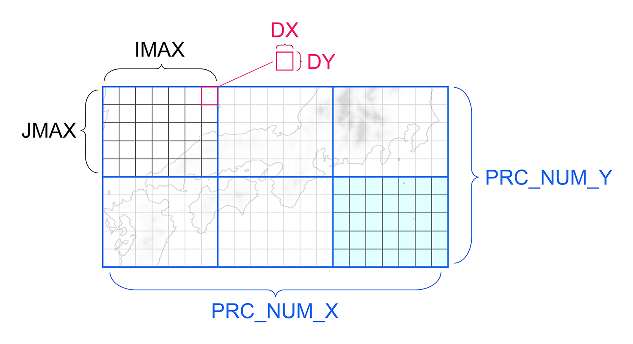
\includegraphics[width=0.8\hsize]{./figure/domain_decomposition.eps}\\
  \caption{計算領域に対する、水平格子間隔(DX, DY)、1MPIプロセスあたりの格子数(IMAX, JMAX)、MPIプロセス数(PRC\_NUM\_X, PRC\_NUM\_Y)の関係。
水色領域は、ある1つのMPIプロセスが担当する領域。}
  \label{fig:domain}
\end{center}
\end{figure}

\subsection{\SubsecDomainSetting} \label{subsec:relation_dom_reso2}

\ref{subsec:relation_dom_reso}節で述べた関係が理解できれば、領域の設定は容易である。
すなわち、式(\ref{eq:xgridnum},\ref{eq:ygridnum})を使って、
\begin{eqnarray}
&& {\XDIR} の領域の長さ = {\XDIR} の格子点数 \times \verb|DX| \nonumber\\
&& {\YDIR}の領域の長さ = {\YDIR}の格子点数 \times \verb|DY| \nonumber
\end{eqnarray}
となる。ここで、\nmitem{DX,DY}は、後述するように
\namelist{PRAM_GRID}で指定されるものである。
逆算して、解像度と領域の大きさをを決めて、MPIプロセス数が決まると、
ローカルな領域の格子点数が決まる。

\subsection{MPIプロセス数} \label{subsec:relation_dom_reso3}

MPIプロセス数は、設定ファイルの\namelist{PARAM_PRC}で指定する。
先に述べた通り、SCALEの入出力ファイルは、MPIプロセス毎に分割されている。
そのため、MPIプロセス数を変更すると分割ファイル数も必ず変わることになる。
従って、例えば、2-MPI並列用に作成した初期値ファイルは、
4-MPI並列のモデル実行には使用できない。
MPIプロセス数を変更するには、
\verb|pp_***.conf|、\verb|init_***.conf|、\verb|run_***.conf| の
すべてを編集・変更し、\verb|pp|, \verb|init| から行う必要がある。\\

\noindent {\small {\gt
\ovalbox{
\begin{tabularx}{140mm}{lX}
\verb|&PARAM_PRC| & \\
\verb| PRC_NUM_X       = 2,| & ; {\XDIR} (東西方向)のMPI並列分割数 \\
\verb| PRC_NUM_Y       = 1,| & ; {\YDIR}(南北方向)のMPI並列分割数 \\
\verb|/|\\
\end{tabularx}
}}}\\


全MPIプロセス数は、\verb|PRC_NUM_X| $\times$ \verb|PRC_NUM_Y|  となり、
上記の例では、$x$方向に2分割、$y$方向に1分割(分割なし)の
2-MPI並列ということになる。

実行時にMPIコマンドに指定するMPIプロセス数は、
この総MPIプロセス数を指定しなければならない。
この条件を満たさない場合は、下記のメッセージが
LOGファイルなどに出力されて計算は行われず、直ちに終了する。

\noindent {\small {\gt
\ovalbox{
\begin{tabularx}{140mm}{l}
\verb|xxx total number of node does not match that requested. Check!| \\
\end{tabularx}
}}}\\





\subsection{\SubsecGridNumSettng} \label{subsec:relation_dom_reso4}
%-----------------------------------------------------------------------

格子数の設定は、設定ファイル(\verb|***.conf|)の\namelist{PARAM_INDEX}で行う。
\ref{subsec:relation_dom_reso}で詳しく説明したように、以下で設定する水平格子数の値は、
1つのMPIプロセス当たりの値であることに注意が必要である。\\

\noindent {\small {\gt
\ovalbox{
\begin{tabularx}{140mm}{lX}
\verb|&PARAM_INDEX| & \\
\verb| KMAX = 97,|  & 鉛直層数 \\
\verb| IMAX = 20,|  & プロセスあたりの{\XDIR} の格子点数 \\
\verb| JMAX = 25,|  & プロセスあたりの{\YDIR}の格子点数 \\
\verb|/|\\
\end{tabularx}
}}}\\



\subsection{\SubsecGridIntvSettng} \label{subsec:gridinterv}
%-----------------------------------------------------------------------
SCALE-RMでは、水平方向には格子点の位置を均等間隔に設定する。
鉛直方向には均等間隔でも任意の格子点位置を直接指定することもできる。
以下で説明する
\textcolor{red}{\bf 格子間隔の設定は、pp\_***.conf、init\_***.conf、run\_***.confの
設定ファイルの間で一致させなければならないことに注意が必要である。}
\ref{subsec:relation_dom_reso}節で述べたように、
以下で設定する値は、MPIプロセス当たりの値であることに注意が必要である。

%-----------------------------------------------------------------------&
第\ref{subsec:buffer}節で述べる緩和領域を覗き、
水平格子間隔は等間隔でしか設定できない。
鉛直格子間隔については、任意に定義することが可能である。
すべての方向について等間隔で設定する場合には、以下のように
設定ファイルの\namelist{PARAM_GRID}の\nmitem{DX,DY,DZ}に
それぞれ、東西、南北、鉛直方向の格子間隔を指定する。
単位はmである。

\noindent {\small {\gt
\ovalbox{
\begin{tabularx}{140mm}{lX}
\verb|&PARAM_GRID  | & \\
\verb| DX = 500.D0,| & ; {\XDIR} (東西方向)の格子間隔\\
\verb| DY = 500.D0,| & ; {\YDIR}(南北方向)の格子間隔\\
\verb| DZ = 500.D0,| & ; {\ZDIR}(鉛直方向)の格子間隔\\
\verb|/|\\
\end{tabularx}
}}}\\


以下に、鉛直方向での任意の格子点位置を指定する場合の設定を示す。
鉛直方向は、Lorenz格子を採用しており、
速度成分定義格子点とスカラー定義格子点が半格子分ずれた食い違い格子にになっている。
ここでは、スカラー量を定義している格子点をセンターポイントと呼び、
半格子ズレた格子点をフェイスポイントと呼ぶ(図\ref{fig:scale_grid}参照)。

直接格子点の位置を指定する場合は、フェイスポイントの位置を
\namelist{PARAM_GRID}の中の\nmitem{FZ(:)}で配列として与えればよい。
\footnote{指定の際には、シミュレーションの計算精度
(モデルのコンパイル時に指定した浮動小数点の精度。デフォルトでは倍精度)を用いることが望ましい。}
また、\nmitem{FZ(:)}で指定する値の数は、鉛直層数
(\namelist{PARAM_INDEX}の\nmitem{KMAX})と一致させる必要がある。
例として理想実験のチュートリアルのrun.confファイル
(run\_R20kmDX500m.conf)を下記に示す。

\noindent {\small {\gt
\ovalbox{
\begin{tabularx}{140mm}{lX}
\verb|&PARAM_GRID|     & \\
\verb| DX = 500.D0,|   & {\XDIR} の格子間隔(等間隔)[m]\\
\verb| DY = 500.D0,|   & {\YDIR}の格子間隔(等間隔)[m]\\
\verb| FZ(:) = |       & {\ZDIR}のフェイスポイントの位置[m] \\
\verb|    80.000000000000000      ,| & \\
\verb|    168.00000190734863      ,| & \\
\verb|    264.80000610351567      ,| & \\
\verb|     〜 中略 〜|           & \\
\verb|    14910.428862936289      ,| & \\
\verb|    15517.262523292475      ,| & \\
\verb|    16215.121232702089      ,| & \\
\verb|    17017.658748523147      ,| & \\
\verb|    17940.576891717363      ,| & \\
\verb|    19001.932756390710      ,| & \\
\verb|    20222.492000765058      ,| & \\
\verb| BUFFER_DZ = 5000.D0,|          & 第\ref{subsec:buffer}節参照\\
\verb| BUFFFACT  =   1.0D0,|          & 第\ref{subsec:buffer}節参照\\
\verb|/|\\
\end{tabularx}
}}}\\


\begin{figure}[tb]
\begin{center}
  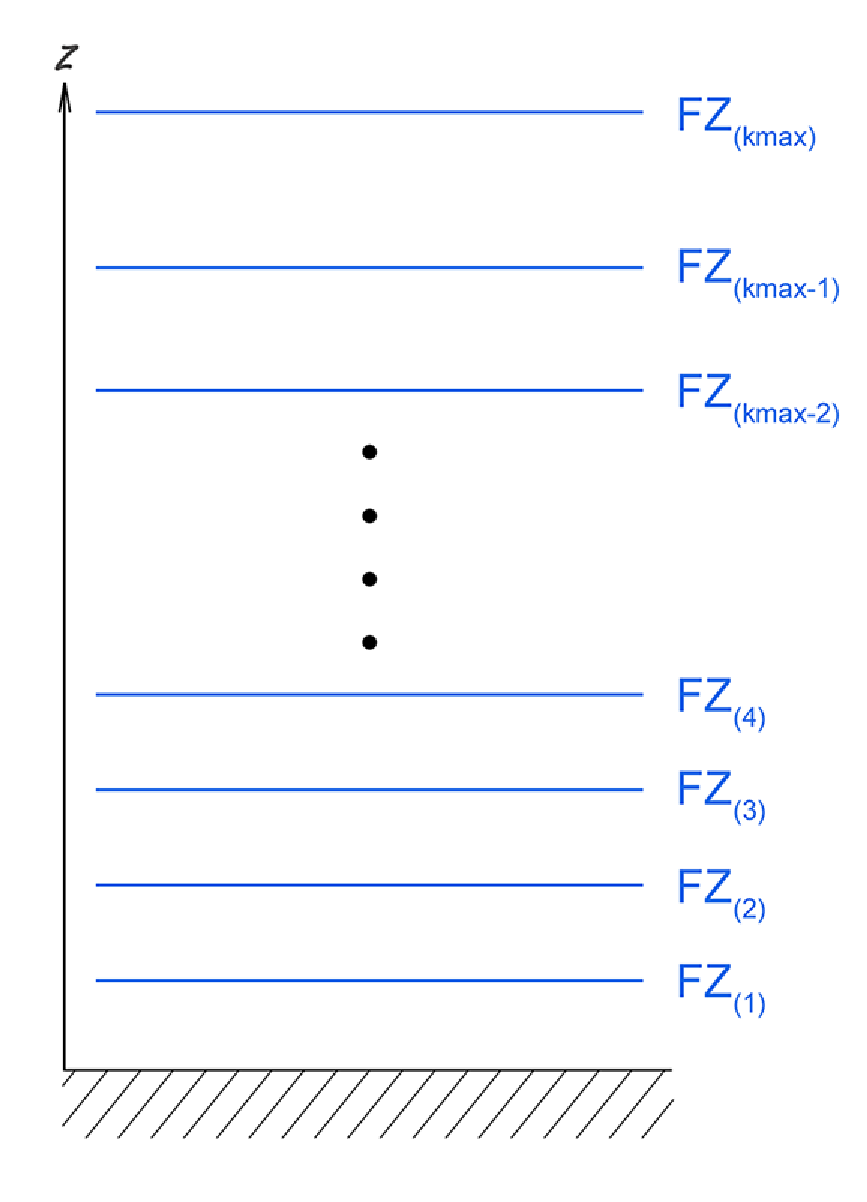
\includegraphics[width=0.4\hsize]{./figure/verticalface.eps}\\
  \caption{SCALE-RMの鉛直格子の定義点。\namelist{PARAM_GRID}で\nmitem{FZ}を指定する時は、ハロを除いた計算領域下端の格子から$k=1$として与える。}
  \label{fig:scale_grid}
\end{center}
\end{figure}
なお、これらの指定では、
標高0mでの格子点として設定され、標高を持つ位置では山岳に沿った座標系によって適切に処理される。


格子点位置は任意に設定できるが、場合によっては計算不安定につながる。
鉛直層の設定については、作成をサポートするツール(\verb|scale/scale-rm/util/makevgrid/|)が
用意されているので参考にされたい。
\footnote{``make\_vgrid.f90''というFortranプログラムと
いくつかのサンプルnamelistが用意されている。}
ツールをコンパイルして実行すれば直ちに設定ファイルに貼り付けて使用できる
\nmitem{FZ(:)}の値が作成される。

\section{緩和領域の設定} \label{sec:buffer}
%-----------------------------------------------------------------------
モデル最上層では重力波の反射、
側面境界では現実大気実験/ネスティング実験を行う際に親領域と対象領域の間の不一致が起こる。
この問題を解決するため、「緩和領域」を設ける。
SCALE-RMでは計算領域の境界のすぐ内側に緩和領域を設定することができる。
緩和領域の格子では、指定された値(境界値データ、親領域のデータなど)に対して
ある時定数で緩和される。以下これをナッジングと呼ぶ。
緩和領域の幅は、設定ファイルの\namelist{PARAM_GRID}の中で設定する。
以下に例を示す。
設定はすべての設定ファイルにおいて共通していなければならない。\\

\noindent {\small {\gt
\ovalbox{
\begin{tabularx}{150mm}{lX}
\verb|&PARAM_GRID  |            & \\
 \verb|BUFFER_DZ = 5000.D0,   | & ; {\ZDIR}(モデルトップから下向き方向)の緩和領域の幅 [m]\\
 \verb|BUFFER_DX = 300000.D0, | & ; {\XDIR} (東西方向)の緩和領域の幅 [m]\\
 \verb|BUFFER_DY = 300000.D0, | & ; {\YDIR}(南北方向)の緩和領域の幅 [m]\\
 \verb|BUFFFACT  = 1.D0,      | & ; 緩和領域内の格子間隔に対するストレッチ係数(デフォルトは1.0)\\
\verb|/|\\
\end{tabularx}
}}}\\

水平方向には東西南北の四方境界に緩和領域が設定されるが、
鉛直方向には計算領域の上端にのみ緩和領域が設定され、下端には設定されない。
%
緩和領域は、計算領域内に設定されるため、
ナッジングの影響を受けない領域(緩和領域を除いた範囲)は
計算領域よりも狭くなることに注意が必要である。

\subsubsection{緩和領域の格子間隔をストレッチさせる}
緩和領域の格子間隔は、基本的に 
\namelist{PARAM_GRID}の中の\nmitem{DX, DY, DZ}で指定した通りであるが、
\nmitem{BUFFFACT}に1以上の値を設定することで、ストレッチさせることも可能である。
ただし、格子間隔を等間隔で指定した場合、
この\nmitem{BUFFFACT}の設定は、x, y, {\ZDIR}すべてに適用されることの注意されたい。
{\ZDIR}の層レベルを任意の格子点位置に指定する場合、
すなわち、\nmitem{FZ(:)}を与える場合(第\ref{subsec:gridinterv}節参照のこと)には適用されない。

緩和領域内の格子間隔 (\verb|BDX|) は次の通り決定される。
\begin{eqnarray}
 \verb|BDX(|n\verb|)| &=& \verb|DX| \times \verb|BUFFFACT|^n \nonumber
\end{eqnarray}
ここで、$n$は緩和領域内の格子点番号を表し、計算領域の内側から外側へ向かって番号が振られる。
緩和領域の格子間隔は、
\verb|BUFFFACT=1.0|ならば内部領域と同じであり、
\verb|BUFFFACT=1.2|ならば内側から外側(境界)に向かって1.2倍の割合で広がっていく。
\verb|BUFFFACT|はいくつに設定しても良いが、計算の安定性を考慮すると 1.0から1.2 が推奨である。

緩和領域の格子数\verb|ibuff|は、
\begin{eqnarray}
\sum_{n=1}^{\verb|ibuff|} \verb|BDX|(n) \ge \verb|BUFFER_DX| \nonumber
\end{eqnarray}
の関係を満たす最小の整数で自動的に計算される。
%
緩和領域の幅(\nmitem{BUFFER_DX})が同じでも、
\nmitem{BUFFFACT}の値を大きくすると緩和領域に用意される格子数は少なくなる。
ここでは、{\XDIR} の説明をしたが、{\YDIR}、{\ZDIR}も同様である。


一般に、緩和領域の大きさ、緩和格子点の数については、解く問題により、明確な指標はない。
SCALE-RMでは、鉛直方向(計算領域トップ)の緩和格子点は5点以上、
水平方向(側面境界付近)の緩和格子点は20〜40点程度を推奨している。
実験設定や事例によっては、さらに緩和格子点を増やしたり、
ストレッチ係数を用いて緩和領域を広げたり、
ここでは説明しないが
\namelist{PARAM_ATMOS_BOUNDARY}の中の
\nmitem{ATMOS_BOUNDARY_taux,ATMOS_BOUNDARY_tauy}を調整して
緩和領域のナッジング強度を調整したりする必要があるだろう。


\section{\SecBasicTopoSetting} \label{sec:basic_usel_topo}
%-----------------------------------------------------------------------

SCALE-RMでは地形データに対しモデル下端の格子面を傾斜させて地形を表現するTerrain followingを採用している。
力学計算過程において安定的に計算を実行するためには、この地形の傾斜角度が45度以下でなければならない。
水平の最大格子間隔をDX [m]、鉛直の最小格子間隔をDZ [m]とすると、地形傾斜角度θ [deg]は次の式で計算される。

\[ \theta = \arctan( DZ/DX ) * 180/PI \]

地形の設定は、設定ファイルの\namelist{PARAM_CNVTOPO}の中で設定する。
以下に例を示す。

\noindent {\small {\gt
\ovalbox{
\begin{tabularx}{150mm}{lX}
\verb|&PARAM_CNVTOPO  |            & \\
 \verb|CNVTOPO_name            = "GTOPO30", | & ; 使用する地形データ名\\
 \verb|CNVTOPO_smooth_maxslope = 0.229,     | & ; 許容する最大傾斜角度 [deg]\\
 \verb|CNVTOPO_smooth_local    = .true.,    | & ; 傾斜を緩める範囲を最大傾斜角度を超えた格子のみ行うかどうか \\
 \verb|CNVTOPO_smooth_itelim   = 10000,     | & ; 傾斜を緩める際の反復計算回数 \\
 \verb|CNVTOPO_copyparent      = .false.,   | & ; 緩和領域に親ドメインの地形データのコピーするかどうか \\
\verb|/|\\
\end{tabularx}
}}}\\

使用する地形データの名称を与え、地形データを読み込む。
SCALE-RMではGTOPO30、または国土地理院による高精度地形データ(DEM50M)をサポートしている。

設定された地形傾斜角度を超える傾斜が与えられた地形データ内に検出された場合、
それを設定された地形傾斜角度以下になるように、反復計算を用いて徐々に傾斜を緩めていく。
このとき、傾斜を緩める範囲を最大傾斜角度を超えた格子のみ行うか、計算領域全体で行うかを選択することができる。
前者は、最大傾斜角度以内のシャープな地形構造を残すことができるので、細かな地形表現を望む場合に選択する。
最大傾斜角度が小さい場合、反復計算回数が相当に大きな数になる場合があるので、適宜反復計算の最大回数を調整する。

上記の計算式で分かるように、空間解像度が変化すると許容される最大傾斜角度が変化する。
多段ドメインを用いた計算を行う場合、一般的に娘ドメインのほうが空間解像度が細かく、地形もシャープに表現される。
このとき、緩和領域に挿入されるデータが、このシャープな地形表現に対して不整合を起こすことがある。
これを回避するために、親ドメインの地形データを緩和領域にコピーし、不整合を回避するオプションを設定できる。
親ドメインが存在しない場合はこのオプションを必ず.false.に設定しなければならない。

\newpage
\section{積分時間と積分時間間隔の設定} \label{sec:timeintiv}
%------------------------------------------------------
積分時間やタイムステップは、実験の目的や設定によって適切に設定する必要がある。
空間解像度を変えた場合はそれに応じたタイムステップを設定する必要があり、
同じ解像度でも計算不安定を防ぐためにタイムステップを短くすることもある。

積分時間とタイムステップの設定は、
configファイル\verb|run_***.conf|の\verb|PARAM_PRC|の項目を編集することで設定できる。
この項目はモデル本体(\verb|scale-rm|)実行時のみで有効であり、初期化作成時には無効である。\\

\noindent {\small {\gt
\ovalbox{
\begin{tabularx}{140mm}{lX}
\verb|&PARAM_TIME| & \\
\verb| TIME_STARTDATE             = 2014, 8, 10, 0, 0, 0,| & 計算開始の日付:放射過程を用いる実験等で必要\\
\verb| TIME_STARTMS               = 0.D0,  | & 計算開始時刻[mili sec]\\
\verb| TIME_DURATION              = 12.0D0,| & 積分時間[単位は\verb|TIME_DURATION_UNIT|で設定]\\
\verb| TIME_DURATION_UNIT         = "HOUR",| & \verb|TIME_DURATION|の単位\\
\verb| TIME_DT                    = 60.0D0,| & トレーサー移流のタイムステップ\\
\verb| TIME_DT_UNIT               = "SEC", | & \verb|TIME_DT|の単位 \\
\verb| TIME_DT_ATMOS_DYN          = 30.0D0,| & 力学過程計算のタイムステップ\\
\verb| TIME_DT_ATMOS_DYN_UNIT     = "SEC", | & \verb|TIME_DT_ATMOS_DYN|の単位\\
\verb| TIME_DT_ATMOS_PHY_MP       = 60.0D0,| & 雲物理過程のタイムステップ \\
\verb| TIME_DT_ATMOS_PHY_MP_UNIT  = "SEC", | & \verb|TIME_DT_ATMOS_PHY_MP|の単位\\
\verb| TIME_DT_ATMOS_PHY_TB       = 60.0D0,| & 乱流スキームのタイムステップ \\
\verb| TIME_DT_ATMOS_PHY_TB_UNIT  = "SEC", | & \verb|TIME_DT_ATMOS_PHY_TB|の単位\\
\verb| TIME_DT_ATMOS_PHY_RD       = 600.0D0, | & 放射スキームのタイムステップ \\
\verb| TIME_DT_ATMOS_PHY_RD_UNIT  = "SEC",  | & \verb|TIME_DT_ATMOS_PHY_RD|の単位\\
\verb| TIME_DT_ATMOS_PHY_SF       = 60.0D0, | & 大気下端境界(フラックス計算)のタイムステップ\\
\verb| TIME_DT_ATMOS_PHY_SF_UNIT  = "SEC",  | & \verb|TIME_DT_ATMOS_PHY_SF|の単位\\
\verb| TIME_DT_OCEAN              = 300.0D0,| & 海面・海洋スキームのタイムステップ\\
\verb| TIME_DT_OCEAN_UNIT         = "SEC",  | & \verb|TIME_DT_OCEAN|の単位\\
\verb| TIME_DT_LAND               = 300.0D0,| & 陸面スキームのタイムステップ\\
\verb| TIME_DT_LAND_UNIT          = "SEC",  | & \verb|TIME_DT_LAND|の単位\\
\verb| TIME_DT_URBAN              = 300.0D0,| & 都市スキームのタイムステップ\\
\verb| TIME_DT_URBAN_UNIT         = "SEC",  | & \verb|TIME_DT_URBAN|の単位\\
\verb| TIME_DT_ATMOS_RESTART      = 21600.D0, | & リスタートファイル(大気)の出力間隔\\
\verb| TIME_DT_ATMOS_RESTART_UNIT = "SEC",    | & \verb|TIME_DT_ATMOS_RESTART|の単位\\
\verb| TIME_DT_OCEAN_RESTART      = 21600.D0, | & リスタートファイル(海洋)の出力間隔\\
\verb| TIME_DT_OCEAN_RESTART_UNIT = "SEC",    | & \verb|TIME_DT_OCEAN_RESTART|の単位\\
\verb| TIME_DT_LAND_RESTART       = 21600.D0, | & リスタートファイル(陸面)の出力間隔\\
\verb| TIME_DT_LAND_RESTART_UNIT  = "SEC",    | & \verb|TIME_DT_LAND_RESTART|の単位\\
\verb| TIME_DT_URBAN_RESTART      = 21600.D0, | & リスタートファイル(都市)の出力間隔\\
\verb| TIME_DT_URBAN_RESTART_UNIT = "SEC",    | & \verb|TIME_DT_URBAN_RESTART|の単位\\
\verb|/|\\
\end{tabularx}
}}}\\


\verb|TIME_DT| は、トレーサー移流のためのタイムステップであり、
格子間隔と移流速度からクーラン条件(CFL条件)を満たすように決定する。
つまり、格子間隔を移流速度で割った値が取りうる最少値よりも小さな値を設定する。
\verb|TIME_DT_ATMOS_DYN| は、力学変数の時間積分のためのタイムステップであり、音速で制約される。
計算安定性のためには、\verb|ATMOS_DYN_TINTEG_SHORT_TYPE| が \verb|RK4| の場合には
最少格子間隔(HE-VI利用時には水平の最少格子間隔)を 420 m/s で割った値が、
\verb|RK3| の場合には 840 m/s で割った値が目安となる。




\section{出力変数の追加・変更} \label{sec:output}
%====================================================================================
新たな変数をhistoryファイルへ追加するには、正式には次の2段階の手続きが必要である。

\begin{enumerate}
\item ソースファイルに、対象の変数をhistory出力するための設定をする。
未設定の場合、run.confに\namelist{HISTITEM}を追加しても出力されない。
\item run.conf内の設定。各変数をhistoryファイルに出力するかどうかを指定。
コンパイルし直すことなく、実験毎に変更可能。
\end{enumerate}
主要な変数についてはすでに1の手続きは行われているため、2の手続きだけ行えばよい。
2の手続きだけで出力可能な変数については、
付録\ref{achap:histroy_item}にリストアップしてあるので、そちらを参照すること。
以下では、2の手続きについて、説明する。\\

まず、出力ファイルと出力形式について、run.**.confの
\namelist{PARAM_HISTORY}に以下の項目を設定する。\\

\noindent {\small {\gt
\ovalbox{
\begin{tabularx}{140mm}{ll}
\verb|&PARAM_HISTORY| \\
\verb|  HISTORY_DEFAULT_BASENAME  |& \verb| = "[character]",| \\
\verb|  HISTORY_DEFAULT_TINTERVAL |& \verb| = [real],| \\
\verb|  HISTORY_DEFAULT_TUNIT     |& \verb| = "[character]",| \\
\verb|  HISTORY_DEFAULT_TAVERAGE  |& \verb| = [logical],| \\
\verb|  HISTORY_DEFAULT_ZINTERP   |& \verb| = [logical],| \\
\verb|  HISTORY_DEFAULT_DATATYPE  |& \verb| = "[character]",| \\
\verb|  HISTORY_OUTPUT_STEP0      |& \verb| = [logical],| \\
\verb|/| \\
\end{tabularx}
}}}\\

\begin{table}[htb]
\begin{center}
\caption{出力ファイルと出力形式の説明}
\begin{tabularx}{150mm}{|l|X|} \hline
 \rowcolor[gray]{0.9} 設定変数 & 説明 \\ \hline
 \verb|HISTORY_DEFAULT_BASENAME  | & 出力ファイル名。\verb|BASENAME_xxxxxx.nc|に出力される。\verb|xxxxxx|はノード番号。\\ \hline
 \verb|HISTORY_DEFAULT_TINTERVAL | & 出力の時間間隔 \\ \hline
 \verb|HISTORY_DEFAULT_TUNIT     | & \verb|HISTORY_DEFAULT_TINTERVAL|の単位\\ \hline
 \verb|HISTORY_DEFAULT_TAVERAGE  | & \verb|.false.| : 瞬間値、\verb|.true.| : 平均値。平均値の場合、
 出力タイミングの直前の\verb|HISTORY_DEFAULT_TINTERVAL|間の平均値が出力される。\\ \hline
 \verb|HISTORY_DEFAULT_DATATYPE  | & 出力値の型。``REAL4'',``REAL8''など。\\ \hline
 \verb|HISTORY_DEFAULT_ZINTERP   | & 鉛直内挿するかどうか。\verb|.false.| : モデル面出力、\verb|.true.| : Z面に内挿した値として出力。\\ \hline
 \verb|HISTORY_OUTPUT_STEP0      | & 初期時刻(t=0)の値を出力するかどうか。\verb|.true.| :出力、\verb|.false.| : 出力しない。\\ \hline
\end{tabularx}
\label{tab:history_settings}
\end{center}
\end{table}


次に、どの変数を出力するか、また各出力変数毎の出力形式の設定を、
run.**.confの\namelist{HISTITEM}に追加する。
\nmitem{ITEM}に設定された変数が出力される。
\textcolor{blue}{青色文字}の部分はオプションで、
オプション変数が特に指定されていない場合は 
\namelist{PARAM_HISTORY}内の設定が適用される。
つまり、出力は、基本的には \namelist{PARAM_HISTORY}に従って行われるが、
\nmitem{HISTITEM}のオプション設定をすることにより、
各変数ごとに出力形式を指定することが可能である。\\


\noindent {\small {\gt
\ovalbox{
\begin{tabularx}{140mm}{l}
\verb|&HISTITEM|\\
                 \verb| ITEM     = "[character]",| \\
\textcolor{blue}{\verb| BASENAME = "[character]",|} \\
\textcolor{blue}{\verb| TINTERVAL= [real],|} \\
\textcolor{blue}{\verb| TUNIT    = "[character]", |} \\
\textcolor{blue}{\verb| TAVERAGE = [logical],|} \\
\textcolor{blue}{\verb| ZINTERP  = [logical], |} \\
\textcolor{blue}{\verb| DATATYPE = "[character]",|} \\
\verb|/| \\
\end{tabularx}
}}}\\


\begin{table}[htb]
\begin{center}
\caption{出力ファイルと出力形式の説明}
\begin{tabularx}{150mm}{|l|X|} \hline
 \rowcolor[gray]{0.9} 設定変数 & 説明 \\ \hline
 \verb|ITEM      | & 変数名。 付録\ref{achap:histroy_item}を参照\\ \hline
 \verb|BASENAME  | & \verb|HISTORY_DEFAULT_BASENAME|に同じ。ただし、変数(\verb|ITEM|)のみに適用。\\ \hline
 \verb|TINTERVAL | & \verb|HISTORY_DEFAULT_TINTERVAL|に同じ。ただし、変数(\verb|ITEM|)のみに適用。\\ \hline
 \verb|TUNIT     | & \verb|TINTERVAL|で指定した出力間隔の単位。\\ \hline
 \verb|TAVERAGE  | & \verb|HISTORY_DEFAULT_TAVERAGE|に同じ。ただし、変数(\verb|ITEM|)のみに適用。\\ \hline
 \verb|DATATYPE  | & \verb|HISTORY_DEFAULT_DATATYPE|に同じ。ただし、変数(\verb|ITEM|)のみに適用。\\ \hline
 \verb|ZINTERP   | & \verb|HISTORY_DEFAULT_ZINTERP|に同じ。ただし、変数(\verb|ITEM|)のみに適用。\\ \hline
\end{tabularx}
\label{tab:histitem}
\end{center}
\end{table}



下記に記述例を示す。
下記の設定では、\verb|history_d03.xxxxxx.nc|に4バイト実数で、
3600秒毎に\verb|HISTITEM|に指定されている変数が出力される。
ただし、``RAIN''については、600秒の出力間隔で、
前600秒の平均値として出力されることを意味している。\\

\noindent {\small {\gt
\ovalbox{
\begin{tabularx}{140mm}{l}
\verb|&PARAM_HISTORY| \\
\verb|  HISTORY_DEFAULT_BASENAME  = "history_d03",| \\
\verb|  HISTORY_DEFAULT_TINTERVAL = 3600.D0,| \\
\verb|  HISTORY_DEFAULT_TUNIT     = "SEC",| \\
\verb|  HISTORY_DEFAULT_TAVERAGE  = .false.,| \\
\verb|  HISTORY_DEFAULT_DATATYPE  = "REAL4",| \\
\verb|  HISTORY_DEFAULT_ZINTERP   = .false.,| \\
\verb|  HISTORY_OUTPUT_STEP0      = .true.,| \\
\verb|/| \\
 \\
\verb|&HISTITEM item="T"    /| \\
\verb|&HISTITEM item="PRES" /| \\
\verb|&HISTITEM item="U"    /| \\
\verb|&HISTITEM item="V"    /| \\
\verb|     〜 中略 〜|\\
\verb|&HISTITEM item="RAIN", taverage=.true., tinterval=600.D0 /| \\
\end{tabularx}
}}}\\


%%%%%%%%%%%%%%%%%%%%%%%%%%%%%%%%%%%%%%%%%%%%%%%%%%%%%%%%%%%%%%%%%%%%%%%%%%%%%%%%%%%%

\section{力学スキームの設定} \label{sec:atmos_dyn}
%------------------------------------------------------


\subsection{数値解法}  \label{subsec:atmos_dyn_sover}
%------------------------------------------------------
時間方向の数値解法選択は、
設定ファイルの\namelist{PARAM_ATMOS}の\nmitem{ATMOS_DYN_TYPE}で行う。\\

\noindent {\gt\small
\ovalbox{
\begin{tabularx}{140mm}{ll}
\verb|&PARAM_ATMOS  | & \\
\verb| ATMOS_DYN_TYPE    = "HEVI", | & ; 表\ref{tab:nml_dyn}より選択。\\
\verb|/             | & \\
\end{tabularx}
}}\\

\begin{table}[h]
\begin{center}
  \caption{数値解法の選択肢}
  \label{tab:nml_dyn}
  \begin{tabularx}{150mm}{llX} \hline
    \rowcolor[gray]{0.9}  設定名 & スキームの説明 & 備考\\ \hline
      \verb|HEVE|  & 水平陽解法-鉛直陽解法 & \\
      \verb|HEVI|  & 水平陽解法-鉛直陰解法 & 推奨(特に実大気実験)\\
    \hline
  \end{tabularx}
\end{center}
\end{table}


\subsection{時間・空間差分スキーム} \label{subsec:atmos_dyn_scheme}
%------------------------------------------------------
時間・空間差分スキームの設定は、設定ファイルの\namelist{PARAM_ATMOS_DYN}で設定する。
また、空間スキームによってはハロの数の設定も必要である。
下記の設定は推奨設定である。
その他、スキームと各種設定については表\ref{tab:nml_atm_dyn}を参照のこと。
また、時間スキーム変更時には、タイムステップも考慮する必要があるが、
それについては、第\ref{sec:timeintiv}節をを参照のこと。\\

\noindent {\gt\small
\ovalbox{
\begin{tabularx}{140mm}{ll}
 \verb|&PARAM_ATMOS_DYN  | & \\
 \verb|ATMOS_DYN_TINTEG_SHORT_TYPE          = RK4,|       & ; 時間スキームより選択\\
 \verb|ATMOS_DYN_TINTEG_TRACER_TYPE         = RK3WS2002,| & ; 時間スキームより選択\\
 \verb|ATMOS_DYN_FVM_FLUX_TYPE              = CD4,|       & ; 空間スキームより選択\\
 \verb|ATMOS_DYN_FVM_FLUX_TRACER_TYPE       = UD3KOREN1993,| & ; 空間スキームより選択\\
 \verb|ATMOS_DYN_FLAG_FCT_TRACER            = .false.,|   & ; FCTスキームを利用するかどうか\\
 \verb|ATMOS_DYN_NUMERICAL_DIFF_COEF        = 1.D-2, |    & \\
 \verb|ATMOS_DYN_NUMERICAL_DIFF_COEF_TRACER = 0.D0, |     & \\
 \verb|ATMOS_DYN_enable_coriolis            = .true.,|    & \\
\verb|/             | & \\
\end{tabularx}
}}\\


\begin{table}[h]
\begin{center}
  \caption{力学スキームの設定}
  \label{tab:nml_atm_dyn}
  \begin{tabularx}{150mm}{llXX} \hline
    \rowcolor[gray]{0.9} & \multicolumn{1}{l}{設定名} & \multicolumn{1}{l}{スキーム名} & \\ \hline
    \multicolumn{3}{l}{時間スキーム} &  \\ \hline
    & \multicolumn{1}{l}{\verb|RK3|} & \multicolumn{2}{l}{3次ルンゲクッタスキーム(Heun)} \\
    & \multicolumn{1}{l}{\verb|RK3WS2002|} & \multicolumn{2}{l}{Wicker and Skamarock (2002) 3段ルンゲクッタスキーム} \\
    & \multicolumn{1}{l}{\verb|RK4|} & \multicolumn{2}{l}{4次ルンゲクッタスキーム} \\
    \hline
    \multicolumn{3}{l}{空間スキーム} & 最小の設定格子数(ハロの数)\\ \hline
    & \multicolumn{1}{l}{\verb|CD2|} & \multicolumn{1}{l}{2次中央差分} & \multicolumn{1}{l}{1}\\
    & \multicolumn{1}{l}{\verb|CD4|} & \multicolumn{1}{l}{4次中央差分} & \multicolumn{1}{l}{2}\\
    & \multicolumn{1}{l}{\verb|CD6|} & \multicolumn{1}{l}{6次中央差分} & \multicolumn{1}{l}{3}\\
    & \multicolumn{1}{l}{\verb|UD3|} & \multicolumn{1}{l}{3次風上差分} & \multicolumn{1}{l}{2}\\
    & \multicolumn{1}{l}{\verb|UD5|} & \multicolumn{1}{l}{5次風上差分} & \multicolumn{1}{l}{3}\\
    & \multicolumn{1}{l}{\verb|UD3KOREN1993|} & \multicolumn{1}{X}{3次風上差分 + Koren(1993)フィルター} & \multicolumn{1}{l}{2}\\
\hline
  \end{tabularx}
\end{center}
\end{table}

トレーサー移流については、何らかの非負保証スキームを使う事が望ましい。\\
つまり \nmitem{ATMOS_DYN_FVM_FLUX_TRACER_TYPE}として \nmitem{UD3KOREN1993}以外を選択した場合は、\\
\nmitem{ATMOS_DYN_FLAG_FCT_TRACER} を \verb|.true.| としてFCTを利用するのがよい。

ハロの数はデフォルトで2となっている。
従って、空間スキームがCD4, UD3以外の場合、上記の表に記したハロの数の設定が必要である。
設定は、\namelist{PARAM_INDEX}の中の\nmitem{IHALO,JHALO}で行う。

例えば、空間スキームに5次風上差分を設定した場合、

\noindent {\gt\small
\ovalbox{
\begin{tabularx}{140mm}{ll}
 \verb|&PARAM_INDEX | &  \\
 \verb| IHALO = 3,|   &\\
 \verb| JHALO = 3,|   &\\
 \verb|/ | & \\
\end{tabularx}
}}\\

のように設定する。

\section{\SecBasicPhysicsSetting} \label{sec:basic_usel_physics}
%------------------------------------------------------

\subsection{\SubsecMicrophysicsSetting} \label{subsec:basic_usel_microphys}
%------------------------------------------------------
雲微物理スキームの選択は、init.confとrun.conf中の
\namelist{PARAM_TRACER}の中の\nmitem{TRACER_TYPE}、
及び、\namelist{PARAM_ATMOS}の\nmitem{ATMOS_PHY_MP_TYPE}で設定する。
このとき{\color{red}{\nmitem{TRACER_TYPE}と\nmitem{ATMOS_PHY_MP_TYPE}は普通は同じものを設定し}}
、かつ、\textcolor{red}{init.conf,run.confで同一の設定}とする必要がある。
ただし、\nmitem{ATMOS_PHY_MP_TYPE}を\verb|OFF|とするときは、\nmitem{TRACER_TYPE}は何を設定してもよいが、乾燥大気の計算をする場合は\verb|TRACER_TYPE = DRY|とするのがよい。
雲微物理スキームを呼び出すタイミングは、
\namelist{PARAM_TIME}で設定するが、これについては
第\ref{sec:timeintiv}節を参照のこと。
以下に、氷雲を含む1-momentバルク法を用いるときの設定を示す。


\noindent {\gt
\ovalbox{
\begin{tabularx}{140mm}{ll}
\verb|&PARAM_ATMOS  | & \\
\verb| ATMOS_PHY_MP_TYPE = "TOMITA08", | & ; 表\ref{tab:nml_atm_mp}より選択。\\
\verb|/             | & \\
\\
\verb|&PARAM_TRACER | & \\
\verb| TRACER_TYPE = "TOMITA08", | & \verb|ATMOS_PHY_MP_TYPE|と同じスキーム。\\
\verb|/             | & \\
\end{tabularx}
}}\\

\begin{table}[h]
\begin{center}
  \caption{雲微物理スキームの設定}
  \label{tab:nml_atm_mp}
  \begin{tabularx}{150mm}{lXX} \hline
    \rowcolor[gray]{0.9}  設定名 & スキームの説明 & 文献\\ \hline
     \verb|OFF|      & 雲微物理による相変化を計算しない &  \\
     \verb|KESSLER|  & 水雲のみの1-momentバルク法 & \citet{kessler_1969} \\
     \verb|TOMITA08| & 氷雲を含む1-momentバルク法 & \citet{tomita_2008} \\
     \verb|SN14|     & 氷雲を含む2-momentバルク法 & \citet{sn_2014} \\
     \verb|SUZUKI10| & 1-momentビン法(氷雲を含むか否かはオプションで選択) & \citet{suzuki_etal_2010} \\
    \hline
  \end{tabularx}
\end{center}
\end{table}

{\color{red}\verb|SUZUKI10|以外を選択する場合}は、
init.conf、run.confの\nmitem{TRACER_TYPE}と\nmitem{ATMOS_PHY_MP_TYPE}を
変更するだけで実行可能であるが、
\verb|SUZUKI10|を選択する場合は、以下のように
init.conf、run.confの双方に
下記を追加する必要がある。\\

\noindent {\gt
\ovalbox{
\begin{tabularx}{140mm}{ll}
\verb|&PARAM_BIN|   &  \\
\verb| nbin   = 33, & (ビンの数)| \\
\verb| ICEFLG =  1, & (氷雲を考慮するか否か,0->水雲のみ,1->氷雲も含む)| \\
\verb|/|            & \\
\end{tabularx}
}}\\

この場合も、
{\color{red}{init.confとrun.confに記載される\verb|PARAM_BIN|は同一にする必要がある}}。
\verb|SUZUKI10|を選択した時には、micpara.datという
雲微物理の計算に必要なファイルが自動生成される。
micpara.datがすでに存在する場合はあるものを利用するが、
nbinが変わると新たに作成しなければならない。
micpara.datの1行目にnbinの情報が記載されているが、
もしrun.confに記載されるnbinと
micpara.datに記載されているnbinが異なれば、\\

\noindent {\gt
\fbox{
\begin{tabularx}{140mm}{l}
\verb|xxx nbin in inc_tracer and nbin in micpara.dat is different check!| \\
\end{tabularx}
}}\\

\noindent というエラーメッセージを標準出力に出力して計算を行わず終了するようになっている。
そのため、nbinを変更した際は、micpara.datを消去して
新たに作り直す必要がある
(micpara.datを消して再度\scalerm をSUZUKI10を用いて実行すれば自動的に新しいmicpara.datが生成される)。



\subsection{\SubsecTurbulenceSetting} \label{subsec:basic_usel_turbulence}
%------------------------------------------------------

乱流スキームの選択は,init.confとrun.conf中の
\namelist{PARAM_ATMOS}の中の\nmitem{ATMOS_PHY_TB_TYPE}で以下のように設定する。
乱流スキームをが呼び出されるタイミングは、
\namelist{PARAM_TIME}で設定するが、これについては
第\ref{sec:timeintiv}節を参照のこと。\\

\noindent {\gt
\ovalbox{
\begin{tabularx}{140mm}{ll}
\verb|&PARAM_ATMOS  | & \\
\verb| ATMOS_PHY_TB_TYPE = "MYNN", | & ; 表\ref{tab:nml_atm_tb}より選択。\\
\verb|/             | & \\
\end{tabularx}
}}\\

\begin{table}[h]
\begin{center}
  \caption{乱流スキームの設定}
  \label{tab:nml_atm_tb}
  \begin{tabularx}{150mm}{lXX} \hline
    \rowcolor[gray]{0.9}  設定名 & スキームの説明 & 文献\\ \hline
      \verb|OFF|          & 乱流の計算を行わない &  \\
      \verb|SMAGORINSKY|  & Smagorinsky 型のサブグリッドモデル    & \citet{smagorinsky_1963,lilly_1962,Brown_etal_1994,Scotti_1993} \\
      \verb|D1980|        & Deardorff(1980)サブグリットモデル &\citet{Deardorff_1980} \\
      \verb|MYNN|         & MYNN Level 2.5 乱流モデル & \citet{my_1982,nakanishi_2004} \\
    \hline
  \end{tabularx}
\end{center}
\end{table}




\subsection{\SubsecRadiationSetting} \label{subsec:basic_usel_radiation}
%-------------------------------------------------------------------------------
放射スキームの選択は、init.confとrun.conf中の
\namelist{PARAM_ATMOS}の\nmitem{ATMOS_PHY_RD_TYPE}で設定する。
放射スキームが呼び出されるタイミングは、\namelist{PARAM_TIME}で設定するが、
これについては第\ref{sec:timeintiv}節を参照のこと。\\

\noindent {\gt
\ovalbox{
\begin{tabularx}{140mm}{ll}
\verb|&PARAM_ATMOS  | & \\
\verb| ATMOS_PHY_RD_TYPE = "MSTRNX", | & ; 表\ref{tab:nml_atm_rd}より選択。\\
\verb|/             | & \\
\end{tabularx}
}}\\

\begin{table}[h]
\begin{center}
  \caption{放射スキームの選択肢}
  \label{tab:nml_atm_rd}
  \begin{tabularx}{150mm}{lXX} \hline
    \rowcolor[gray]{0.9}  設定名 & スキームの説明 & 文献\\ \hline
      \verb|OFFまたはNONE| & 放射スキームを使用しない & \\
      \verb|MSTRNX|       & mstrnX & \citet{sekiguchi_2008} \\
      \verb|WRF|          & mstrnX(長波)+Dudhia(短波) & \citet{dudhia_1989} \\
    \hline
  \end{tabularx}
\end{center}
\end{table}

放射計算のための太陽放射量は、
モデル実行の日付および時刻設定と、モデルの計算領域の緯度経度に従って計算される。
理想実験のために、太陽放射量、緯度経度、時刻を固定することも出来る。
これらは\namelist{PARAM_ATMOS_SOLARINS}で設定する。\\

\noindent {\small {\gt
\ovalbox{
\begin{tabularx}{150mm}{lX}
\verb|&PARAM_ATMOS_SOLARINS        | & \\
\verb| ATMOS_SOLARINS_constant    = 1360.250117   | & 太陽定数 [W/m2] \\
\verb| ATMOS_SOLARINS_fixedlatlon = .false.       | & 放射計算の緯度経度を固定するかどうか\\
\verb| ATMOS_SOLARINS_fixeddate   = .false.       | & 放射計算の日時を固定するかどうか\\
\verb| ATMOS_SOLARINS_lon         = 135.221       | & \verb|ATMOS_SOLARINS_fixedlatlon=.true.|の場合の経度 [deg.] \\
\verb| ATMOS_SOLARINS_lat         =  34.653       | & \verb|ATMOS_SOLARINS_fixedlatlon=.true.|の場合の緯度 [deg.]\\
\verb| ATMOS_SOLARINS_date = -1,-1,-1,-1,-1,-1,   | & \verb|ATMOS_SOLARINS_fixeddate=.true.|の場合の年月日時刻 [Y,M,D,H,M,S]\\
\verb|/|            & \\
\end{tabularx}
}}}\\

上記は初期値を示している。
\namelist{PARAM_MAPPROJ}の\nmitem{MPRJ_basepoint_lon,MPRJ_basepoint_lat}が設定されている場合には、
\nmitem{ATMOS_SOLARINS_lon,ATMOS_SOLARINS_lat}の初期値は、\\
\nmitem{MPRJ_basepoint_lon,MPRJ_basepoint_lat}がそれぞれ与えられる。


実験設定によっては、モデルトップの高度が10-20 kmと低いことがしばしばある。
そのため放射計算ではモデルトップとは別の最上層高度を設定し、
モデルトップより上空を何層で表現するか設定するようになっている。
放射用最上層を何kmにとるかは放射スキーム依存であるが、
例えば\verb|MSTRNX|ではデフォルトの
パラメータテーブルが想定する放射用最上層は100kmである。
追加される高度はデフォルトの場合10層で表現する。
すなわち、モデルトップが22kmであれば、放射スキーム内では
7.8km$\times$10層が追加されて計算される。
これらは\verb|MSTRNX|なら\namelist{PARAM_ATMOS_PHY_RD_MSTRN}で設定する。\\

\noindent {\small {\gt
\ovalbox{
\begin{tabularx}{150mm}{lX}
\verb|&PARAM_ATMOS_PHY_RD_MSTRN | & \\
\verb| ATMOS_PHY_RD_MSTRN_KADD                  = 10 | & モデルトップから大気トップまでの間の放射計算用の層数 \\
\verb| ATMOS_PHY_RD_MSTRN_GASPARA_IN_FILENAME   = "PARAG.29"     | & ガスパラメータの入力ファイル \\
\verb| ATMOS_PHY_RD_MSTRN_AEROPARA_IN_FILENAME  = "PARAPC.29"    | & エアロゾルパラメータの入力ファイル\\ 
\verb| ATMOS_PHY_RD_MSTRN_HYGROPARA_IN_FILENAME = "VARDATA.RM29" | & 吸湿性エアロゾルパラメータの入力ファイル\\
\verb| ATMOS_PHY_RD_MSTRN_nband                 = 29             | &  wave bands\\
\verb| ATMOS_PHY_RD_MSTRN_nptype                = 11             | & エアロゾルの種類の数\\
\verb| ATMOS_PHY_RD_MSTRN_nradius               = 6              | & radius mode for hygroscopic parameter\\
\verb| ATMOS_PHY_RD_MSTRN_ONLY_QCI              = .false.        | & ? \\
\verb|/| & \\
\end{tabularx}
}}}\\

\verb|MSTRNX|を実行するには、放射計算のためのパラメータテーブルが必要である。
デフォルトでは太陽放射から赤外放射までを29バンド111チャンネルに分割し、
雲・エアロゾル粒子の粒径を6ビンで表した時のテーブルを用いている。
パラメータファイル(3種類)も、
\begin{verbatim}
  scale-rm/test/data/rad/
\end{verbatim}
に用意されている。
\namelist{PARAM_ATMOS_PHY_RD_MSTRN}でファイルのディレクトリと名前を指定する。

追加された層の気温・気圧プロファイルは外部から与える必要がある。
また二酸化炭素やオゾン等の気体濃度プロファイルも必要である。
\scalerm では気温・気圧についてはCIRA86
\footnote{http://catalogue.ceda.ac.uk/uuid/4996e5b2f53ce0b1f2072adadaeda262}\citep{CSR_2006}、
気体種についてはMIPAS2001\citep{Remedios_2007}の気候値を用意している。
気候値プロファイルについても、
モデル実行の日付および時刻設定とモデルの計算領域の緯度経度に従って計算される。
読み込むファイルは、
\begin{verbatim}
  scale-rm/test/data/rad/
\end{verbatim}
に用意されており、\namelist{PARAM_ATMOS_PHY_RD_PROFILE}でファイルのディレクトリと名前を指定する。\\


\noindent {\small {\gt
\ovalbox{
\begin{tabularx}{150mm}{lX}
\verb|&PARAM_ATMOS_PHY_RD_PROFILE | & \\
\verb| ATMOS_PHY_RD_PROFILE_TOA                   = 100.0     | & 大気最上層(TOA)の高さ [km] \\
\verb| ATMOS_PHY_RD_PROFILE_use_climatology       = .true.    | & \textcolor{red}{具体的にどういうこと?}\\
\verb| ATMOS_PHY_RD_PROFILE_CIRA86_IN_FILENAME    = "cira.nc" | & \verb|CIRA86 (NetCDF format)|ファイル  \\
\verb| ATMOS_PHY_RD_PROFILE_MIPAS2001_IN_BASENAME = "."       | & \verb|MIPAS2001 (ASCII format)|のディレクトリの場所 \\
\verb| ATMOS_PHY_RD_PROFILE_USER_IN_FILENAME      = ""        | & (user,ASCII format) \textcolor{red}{これ、使えますか?} \\
\verb| ATMOS_PHY_RD_PROFILE_USE_CO2               = .true.    | & \textcolor{red}{falseにするとどうなる?}\\
\verb| ATMOS_PHY_RD_PROFILE_USE_O3                = .true.    | & \\
\verb| ATMOS_PHY_RD_PROFILE_USE_N2O               = .true.    | & \\
\verb| ATMOS_PHY_RD_PROFILE_USE_CO                = .true.    | & \\
\verb| ATMOS_PHY_RD_PROFILE_USE_CH4               = .true.    | & \\
\verb| ATMOS_PHY_RD_PROFILE_USE_O2                = .true.    | & \\
\verb| ATMOS_PHY_RD_PROFILE_USE_CFC               = .true.    | & \\
\verb|/| & \\
\end{tabularx}
}}}\\



\subsection{\SubsecSurfaceSetting} \label{subsec:basic_usel_surface}
%------------------------------------------------------
大気下端境界の選択は、init.confとrun.conf中の
\namelist{PARAM_ATMOS}の\nmitem{ATMOS_PHY_SF_TYPE}で以下のように設定する。
海面・陸面・都市モデルを用いない場合の
大気下端境界のフラックススキームが呼び出されるタイミングは、
\namelist{PARAM_TIME}で設定する。
時間設定の詳細については第\ref{sec:timeintiv}節を参照のこと。\\

\noindent {\gt
\ovalbox{
\begin{tabularx}{140mm}{ll}
\verb|&PARAM_ATMOS  | & \\
\verb| ATMOS_PHY_SF_TYPE = "COUPLE", | & ; 表\ref{tab:nml_atm_sf}より選択。\\
\verb|/             | & \\
\end{tabularx}
}}\\

\begin{table}[h]
\begin{center}
  \caption{大気下端境界の選択肢}
  \label{tab:nml_atm_sf}
  \begin{tabularx}{150mm}{lX} \hline
    \rowcolor[gray]{0.9}  設定名 & スキームの説明\\ \hline
      \verb|OFFまたはNONE| & 地表面フラックスを計算しない \\
      \verb|CONST|      & 地表面フラックスを任意の値に固定 \\
      \verb|BULK|       & 地表面フラックスをバルクモデルで計算 \\
      \verb|COUPLE|     & 海面・陸面・都市モデルそれぞれが計算するフラックスを受け取る \\
    \hline
  \end{tabularx}
\end{center}
\end{table}


%-------------------------------------------------------------------------------
\subsubsection{一定値設定の場合}

\nmitem{ATMOS_PHY_SF_TYPE = "CONST"}を選択した場合は、run.confで
下記を設定することにより、
任意の値に固定することが可能である。下記の値はデフォルトの設定を示す。\\

\noindent {\small {\gt
\ovalbox{
\begin{tabularx}{150mm}{lX}
 \\
 \verb|&PARAM_ATMOS_PHY_SF_CONST                | & \\
 \verb| ATMOS_PHY_SF_FLG_MOM_FLUX   =    0      | & 0: バルク係数を一定にする時 \\
                                                  &            1: 摩擦速度を一定にする時 \\
 \verb| ATMOS_PHY_SF_U_minM         =    0.0D0  | & 絶対速度の下限値 [m/s] \\
 \verb| ATMOS_PHY_SF_Const_Cm       = 0.0011D0  | & 運動量に対する一定バルク係数値 \\
                                                  &  (\verb|ATMOS_PHY_SF_FLG_MOM_FLUX = 0| のとき有効) \\
 \verb| ATMOS_PHY_SF_CM_min         = 1.0D-5    | & 運動量に対するバルク係数の下限値 \\
                                                  &  (\verb|ATMOS_PHY_SF_FLG_MOM_FLUX = 1| のとき有効) \\
 \verb| ATMOS_PHY_SF_Const_Ustar    =   0.25D0  | & 一定摩擦係数値 [m/s] \\
                                                  &  (\verb|ATMOS_PHY_SF_FLG_MOM_FLUX = 1| のとき有効) \\
 \verb| ATMOS_PHY_SF_Const_SH       =   15.0D0  | & 一定地表面顕熱フラックス値 [W/m2] \\
 \verb| ATMOS_PHY_SF_FLG_SH_DIURNAL =  .false.  | & 顕熱フラックスに日変化をつけるか否か [logical]\\
 \verb| ATMOS_PHY_SF_Const_FREQ     =   24.0D0  | & 顕熱フラックスに日変化を付けるときのサイクル [hour]\\
 \verb| ATMOS_PHY_SF_Const_LH       =  115.0D0  | & 一定地表面潜熱フラックス値 [W/m2] \\
 \verb|/|            & \\
 \\
\end{tabularx}
}}}\\

\subsubsection{バルク設定の場合}
%-------------------------------------------------------------------------------
\nmitem{ATMOS_PHY_SF_TYPE = "BULK"}を選択した場合は、
任意の地表面温度に対応したフラックスをバルクモデルに従って計算する。
これは海洋・陸面・都市モデルを用いずに下端境界を設定する際(特に理想実験)に利用される。
このとき、粗度は海面粗度の計算スキームを利用しているが、
後述するように海面粗度は定数を与えることができ、
また蒸発効率を決める係数も任意の値を設定出来るため、
海面に限定せず、陸面を想定した理想実験も行うことが出来る。

海面粗度を計算するスキームは、
run.conf中の\namelist{PARAM_ROUGHNESS}の\nmitem{ROUGHNESS_TYPE}で以下のように設定する。\\

\noindent {\gt
\ovalbox{
\begin{tabularx}{140mm}{ll}
\verb|&PARAM_ROUGHNESS  | & \\
\verb| ROUGHNESS_TYPE = "MOON07", | & ; 表\ref{tab:nml_roughness}より選択。\\
\verb|/             | & \\
\end{tabularx}
}}\\

\begin{table}[h]
\begin{center}
  \caption{海面粗度スキームの選択肢}
  \label{tab:nml_roughness}
  \begin{tabularx}{150mm}{llX} \hline
    \rowcolor[gray]{0.9}  設定名 & スキームの説明 & 文献 \\ \hline
      \verb|MOON07|   & デフォルト & \citet{moon_2007} \\
      \verb|MILLER92| &            & \citet{miller_1992} \\
      \verb|CONST|    & 定数を与える & \\
    \hline
  \end{tabularx}
\end{center}
\end{table}

また、フラックス計算に使用するバルク交換係数の計算スキームは
run.conf中の\namelist{PARAM_BULKFLUX}の\nmitem{BULKFLUX_TYPE}で以下のように設定する。\\

\noindent {\gt
\ovalbox{
\begin{tabularx}{140mm}{ll}
\verb|&PARAM_BULKFLUX  | & \\
\verb| BULKFLUX_TYPE = "B91W01", | & ; 表\ref{tab:nml_bulk}より選択。\\
\verb|/             | & \\
\end{tabularx}
}}\\

\begin{table}[h]
\begin{center}
  \caption{バルクフラックススキームの選択肢}
  \label{tab:nml_bulk}
  \begin{tabularx}{150mm}{llX} \hline
    \rowcolor[gray]{0.9}  設定名 & スキームの説明 & 文献 \\ \hline
      \verb|B91W01| & デフォルト & \citet{beljaars_1991,wilson_2001} \\
      \verb|U95|    &          & \citet{uno_1995} \\
    \hline
  \end{tabularx}
\end{center}
\end{table}



\subsection{\SubsecOceanSetting} \label{subsecp:basic_usel_ocean}
%-------------------------------------------------------------------------------
海洋過程は海面の状態量の更新と大気ー海洋間のフラックス計算の2つに大別される。
これらの過程を計算するタイミングはどちらも\namelist{PARAM_TIME}で設定する。
時間設定の詳細については第\ref{sec:timeintiv}節を参照のこと。\\


\subsubsection{海面スキーム}
%-------------------------------------------------------------------------------
海面の状態量(主に海面温度)の更新を担う海面スキームの選択は、init.confとrun.conf中の
\namelist{PARAM_OCEAN}の\nmitem{OCEAN_TYPE}で設定する。\\
海面のアルベドは、どの海面スキームを選択しても同じ計算スキームが適用され、
太陽天頂角に応じたアルベドが計算される。

\noindent {\gt
\ovalbox{
\begin{tabularx}{140mm}{ll}
\verb|&PARAM_OCEAN           | & \\
\verb| OCEAN_TYPE = "CONST", | & ; 表\ref{tab:nml_ocean}より選択。\\
\verb|/                      | & \\
\end{tabularx}
}}\\

\begin{table}[h]
\begin{center}
  \caption{海洋スキームの選択肢}
  \label{tab:nml_ocean}
  \begin{tabularx}{150mm}{lX} \hline
    \rowcolor[gray]{0.9}  設定名 & スキームの説明                        \\ \hline
      \verb|NONEまたはOFF|       & 土地利用にOCEANがない場合のみ使用可   \\
      \verb|CONST|               & 初期値のまま固定                      \\
      \verb|FILE|                & 外部ファイルから与える (時間変化あり) \\
      \verb|SLAB|                & スラブ海洋モデル                      \\
    \hline
  \end{tabularx}
\end{center}
\end{table}


\verb|OCEAN_TYPE = "FILE"|を選択した場合は、init.confとrun.confで外部入力ファイルの設定が必要である。
この場合、与えられた外部ファイルの空間部分布と時系列に応じて、海面温度は変化する。\\

\noindent {\gt
\ovalbox{
\begin{tabularx}{140mm}{ll}
 \verb|&EXTITEM                                  | & \\
 \verb| basename   = "../init/output/ocean_d01", | & ; 入力ファイル\\
 \verb| varname    = "OCEAN_TEMP",               | & ; \verb|"OCEAN_TEMP"|と書く。\\
 \verb| step_limit = 1800,                       | & \\
 \verb| step_fixed =  -1,                        | & \\
 \verb| enable_periodic_year  = .false.,         | & \\
 \verb| enable_periodic_month = .false.,         | & \\
 \verb| enable_periodic_day   = .false.,         | & \\
 \verb|/                                         | & \\
\end{tabularx}
}}\\


\verb|OCEAN_TYPE = "SLAB"|を選択した場合は、init.confとrun.confでスラブ混合層の深さを設定することができる。
この場合、大気-海洋間の熱フラックスの移動に応じて、スラブ混合層の温度は時間発展する。\\

\noindent {\gt
\ovalbox{
\begin{tabularx}{140mm}{ll}
 \verb|&PARAM_OCEAN_PHY_SLAB            | & \\
 \verb|  OCEAN_PHY_SLAB_DEPTH = 10.0D0, | & ; デフォルト設定[m] \\
 \verb|/                                | & \\
\end{tabularx}
}}\\

\subsubsection{大気-海洋フラックス}
%-------------------------------------------------------------------------------
海面スキームで計算された大気ー海洋間フラックスを大気に反映させるには、
\namelist{PARAM_ATMOS}で\nmitem{ATMOS_PHY_SF_TYPE = "COUPLE"}とする必要がある。\\

\noindent {\gt
\ovalbox{
\begin{tabularx}{140mm}{ll}
\verb|&PARAM_ATMOS  | & \\
\verb| ATMOS_PHY_SF_TYPE = "COUPLE", | &\\
\verb|/             | & \\
\end{tabularx}
}}\\

大気ー海洋間フラックスは、複数あるバルクスキームのいずれかを用いて計算される。
また、バルクスキーム内で利用される海面粗度長計算についても、複数のスキームが選択できる。\\

海面粗度を計算するスキームは、
run.conf中の\namelist{PARAM_ROUGHNESS}の\nmitem{ROUGHNESS_TYPE}で設定する。

フラックス計算に使用するバルク交換係数の計算スキームは
run.conf中の\namelist{PARAM_BULKFLUX}の\nmitem{BULKFLUX_TYPE}で設定する。
これらの詳細については、第\ref{subsec:basic_usel_surface}節参照のこと。



\subsection{\SubsecLandSetting} \label{subsec:basic_usel_land}
%-------------------------------------------------------------------------------
陸面過程についても、海洋過程と同じく陸面の状態量の更新と大気ー陸面間のフラックス計算の2つに大別される。
これらの過程が呼び出されるタイミングはどちらも\namelist{PARAM_TIME}で設定する。
時間設定の詳細については第\ref{sec:timeintiv}節を参照のこと。\\


\subsubsection{陸面スキーム}
%-------------------------------------------------------------------------------
陸面の状態量(主に陸面温度と土壌温度、土壌水分量)の更新を担う陸面スキームの選択は、
init.confとrun.conf中の\namelist{PARAM_LAND}の\nmitem{LAND_TYPE}で以下のように設定する。\\

\noindent {\gt
\ovalbox{
\begin{tabularx}{140mm}{ll}
\verb|&PARAM_LAND  | & \\
\verb| LAND_TYPE = "SLAB", | & ; 表\ref{tab:nml_land}より選択。\\
\verb|/             | & \\
\end{tabularx}
}}\\

\begin{table}[h]
\begin{center}
  \caption{陸面スキームの選択肢}
  \label{tab:nml_land}
  \begin{tabularx}{150mm}{llX} \hline
    \rowcolor[gray]{0.9}  設定名 & スキームの説明 \\ \hline
      \verb|NONEまたはOFF| & 土地利用にLANDがない場合のみ使用可            \\
      \verb|SLAB|         & 熱拡散モデル+バケツモデル                    \\
      \verb|CONST|        & SLABで土壌温度、土壌水分量、陸面温度を更新しない \\
    \hline
  \end{tabularx}
\end{center}
\end{table}


\nmitem{LAND_TYPE = "SLAB"}または\nmitem{LAND_TYPE = "CONST"}を選択した場合は、
土地利用区分に応じたアルベド、粗度長等のパラメータテーブルと、土地利用区分分布の入力が必要である。
パラメータテーブルは、
\begin{verbatim}
  scale-rm/test/data/land/param.bucket.conf
\end{verbatim}
に用意されている。\\


\subsubsection{大気-陸面フラックス}
%-------------------------------------------------------------------------------
陸面スキームで計算された大気ー陸面間フラックスを大気に反映させるには、
\namelist{PARAM_ATMOS}で\nmitem{ATMOS_PHY_SF_TYPE = "COUPLE"}とする必要がある。\\

\noindent {\gt
\ovalbox{
\begin{tabularx}{140mm}{ll}
\verb|&PARAM_ATMOS  | & \\
\verb| ATMOS_PHY_SF_TYPE = "COUPLE", | &\\
\verb|/             | & \\
\end{tabularx}
}}\\

大気ー陸面間フラックスの計算スキームは、陸面スキームに対応して選択される。
\nmitem{LAND_TYPE = "SLAB"}または\nmitem{LAND_TYPE = "CONST"}を選択した場合は、
海面または理想実験用の地表面で用いられるバルクスキームと同じものが利用される。\\

この時のフラックス計算に使用するバルク交換係数の計算スキームは
run.conf中の\namelist{PARAM_BULKFLUX}の\nmitem{BULKFLUX_TYPE}で設定する。\\
%%%% 記載必要


\subsection{\SubsecUrbanSetting} \label{subsec:basic_usel_urban}
%------------------------------------------------------
都市モデルを用いる場合、
\namelist{PARAM_ATMOS}において、\nmitem{ATMOS_PHY_SF_TYPE = "COUPLE"}である必要がある。
都市モデルの選択は、init.confとrun.conf中の
\namelist{PARAM_URBAN}の\nmitem{URBAN_TYPE}で以下のように設定する。
都市モデルが呼び出されるタイミングは、
\namelist{PARAM_TIME}で設定するが、これについては
第\ref{sec:timeintiv}節を参照のこと。\\

\noindent {\gt
\ovalbox{
\begin{tabularx}{140mm}{ll}
\verb|&PARAM_ATMOS  | & \\
\verb| ATMOS_PHY_SF_TYPE = "COUPLE", | &\\
\verb|/             | & \\
\\
\verb|&PARAM_URBAN  | & \\
\verb| URBAN_TYPE="SLC", | & ; 表\ref{tab:nml_urban}より選択。\\
\verb|/             | & \\
\end{tabularx}
}}\\

\begin{table}[h]
\begin{center}
  \caption{都市スキームの選択肢}
  \label{tab:nml_urban}
  \begin{tabularx}{150mm}{llX} \hline
    \rowcolor[gray]{0.9}  設定名 & スキームの説明 & 文献\\ \hline
      \verb|OFF|  & 土地利用に都市がない場合のみ使用可 &   \\
      \verb|SLC|  & 単層キャノピーモデル   & \citet{kusaka_2001} \\
    \hline
  \end{tabularx}
\end{center}
\end{table}


\chapter{各種設定: 実用編} \label{chap:advance_use}
\section{概要} \label{sec:advance_use_overview}

この章では、更に発展的な使い方似ついて説明する。
以下に、項目を列挙する。

{
\begin{center}
\begin{tabular}[h]{ll}\hline
\SecAdvanceMapprojectionSetting & 第\ref{sec:adv_mapproj}節 \\
\SecAdvanceInputDataSetting & 第\ref{sec:adv_datainput}節\\
\hline
\end{tabular}
\end{center}
}




\section{\SecAdvanceMapprojectionSetting} \label{sec:adv_mapproj}
%------------------------------------------------------
計算領域の位置と投影法は、設定ファイルの\verb|PARAM_MAPPROJ|の項目を編集することで設定できる。
\textcolor{red}{\bf この設定も、pp\_***.conf、init\_***.conf、run\_***.confの設定ファイルの間で
必ず一致させなければならない。}はじめに下記の例をもとに説明する。\\

\noindent {\small {\gt
\ovalbox{
\begin{tabularx}{140mm}{l}
\verb|&PARAM_MAPPROJ| \\
\verb| MPRJ_basepoint_lon = 138.727778D0,| \\
\verb| MPRJ_basepoint_lat = 35.360556D0,| \\
\verb| MPRJ_type          = 'MER',| \\
\verb|/| \\
\end{tabularx}
}}}\\

\noindent
まず\nmitem{MPRJ_basepoint_lat}と\nmitem{MPRJ_basepoint_lon}は、
計算領域の中心の緯度・経度を表す。
SCALE-RMでは、北緯を正、南緯を負の値として表現し、
経度は0度を起点に右回りで表現するため、
この設定では計算領域の
中心が北緯35.360556度、東経138.727778度に位置することになる。
この場所を中心に指定された大きさで、計算領域が
設定される
\footnote{デフォルトではメルカトル図法に基づいて緯度・経度を計算する際の基準とする緯度は、
\nmitem{MPRJ_basepoint_lat}の値が使用されるが、\nmitem{MPRJ\_M\_lat}を用いて
任意の緯度を指定することもできる。}。
実際にはSCALE-RM内部での格子点は、
実距離に基づいて格子点が配置される。
このため、設定された投影法では、実距離に基づいた緯度・経度座標が計算される。
この緯度・経度情報は、すべてのSCALEのNetCDF形式の出力ファイルに含まれている。

\nmitem{MPRJ_type}は、地図投影法の種類を表しており、\verb|MER|はメルカトル図法を意味する。
SCALEで現在選択できる地図投影法とその指定文字列は表\ref{tab:map_proj}のとおりである。

\begin{table}[tbh]
\begin{center}
\caption{SCALEで選択できる地図投影法}
\begin{tabularx}{150mm}{|l|X|} \hline
 \rowcolor[gray]{0.9} 地図投影法 & \verb|MPRJ_type| \\ \hline
 地図投影なし(理想実験用)& \verb|NONE| \\ \hline
 ランベルト正角円錐図法 & \verb|LC| \\ \hline
 極心平射図法(ポーラーステレオ) & \verb|PS| \\ \hline
 メルカトル図法 & \verb|MER| \\ \hline
 正距円筒図法 & \verb|EC| \\ \hline
\end{tabularx}
\label{tab:map_proj}
\end{center}
\end{table}

ここで、ランベルト正角円錐図法の設定方法については、設定方法が異なるため以下に説明する。
ここでは、現実大気実験チュートリアルで使用した\verb|run.conf|ファイルを例に挙げる。\\

\noindent {\small {\gt
\ovalbox{
\begin{tabularx}{140mm}{l}
\verb|&PARAM_MAPPROJ| \\
\verb| MPRJ_basepoint_lon = 135.220404D0,| \\
\verb| MPRJ_basepoint_lat = 34.653396D0,| \\
\verb| MPRJ_type          = 'LC',| \\
\verb| MPRJ_LC_lat1       =  30.00D0,| \\
\verb| MPRJ_LC_lat2       =  40.00D0,| \\
\verb|/| \\
\end{tabularx}
}}}\\

SCALE-RMでは2標準緯線型の実装を採用しているため、投影を決定する上で2つの標準緯線の
位置を指定する必要がある。2つの標準緯線に挟まれた領域では、
緯線・経線の長さの比が地球楕円体面上における
長さの比と近くなるように調節される。
従って、標準緯線を設定する
\nmitem{MPRJ_LC_lat1}と\nmitem{MPRJ_LC_lat2}の項目が追加されている。
それぞれ、南側、北側の標準緯線の値の単位は、degreeで指定する。

さらに下記のように\nmitem{MPRJ_basepoint_x}と\nmitem{MPRJ_basepoint_y}という変数を用いることで、
地図投影中心と計算領域中心をずらすこともできる。\\

\noindent {\small {\gt
\ovalbox{
\begin{tabularx}{140mm}{l}
\verb|&PARAM_MAPPROJ| \\
\verb| MPRJ_basepoint_lon = 135.220404D0,| \\
\verb| MPRJ_basepoint_lat = 34.653396D0,| \\
\verb| MPRJ_basepoint_x   = 100.0D0,| \\
\verb| MPRJ_basepoint_y   = 100.0D0,| \\
\verb| MPRJ_type          = 'LC',| \\
\verb| MPRJ_LC_lat1       =  30.00D0,| \\
\verb| MPRJ_LC_lat2       =  40.00D0,| \\
\verb|/| \\
\end{tabularx}
}}}\\

\noindent 
\nmitem{MPRJ_basepoint_x}と\nmitem{MPRJ_basepoint_y}は、地図投影中心の位置を、
計算領域の南西端(左下角)からの距離で指定するパラメータで、
単位はメートルである。
これらを指定しない場合は、デフォルト設定として計算領域中心と
地図投影中心の位置は一致する。
上記の場合とデフォルト設定の場合を比較したものを図\ref{fig:map_lc}に示す。
図\ref{fig:map_lc}aはデフォルト設定で投影中心と計算領域中心が一致している場合、
図\ref{fig:map_lc}bは、計算領域の位置を投影中心からずらした場合の関係を表している。
図\ref{fig:map_lc}bでは、計算領域の南西端から
\nmitem{MPRJ_basepoint_x}と\nmitem{MPRJ_basepoint_y}で指定した
距離だけ離れた位置に投影中心がある。

\begin{figure}[t]
\begin{center}
  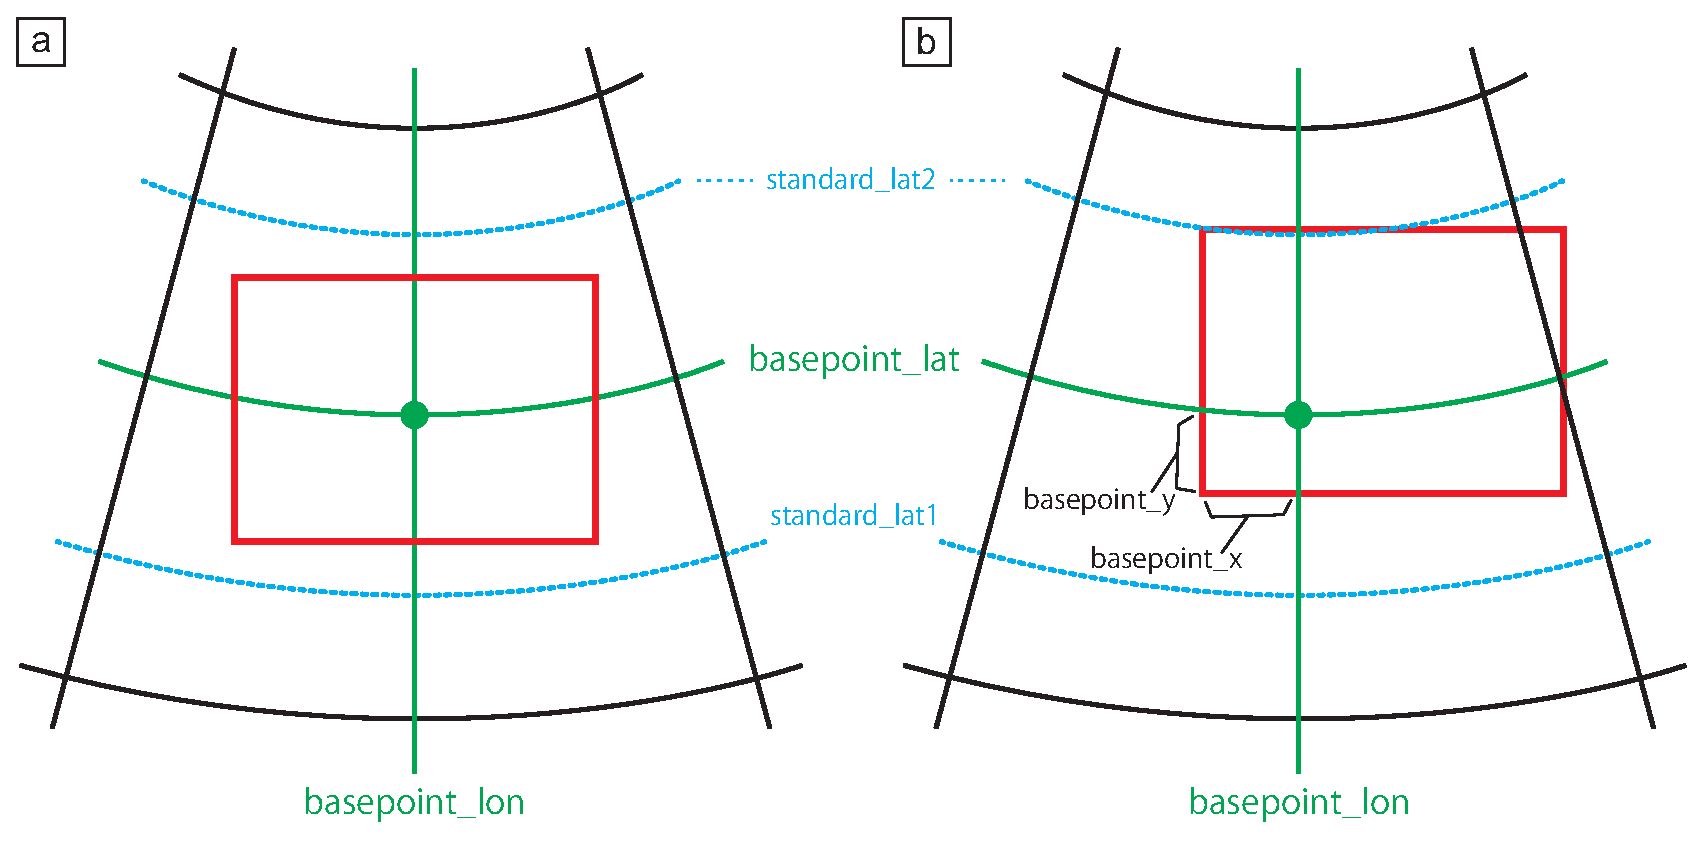
\includegraphics[width=0.8\hsize]{./figure/LC_latlon_xy.eps}\\
  \caption{投影中心と計算領域の関係:(a)はデフォルト設定の場合、(b)は計算領域の位置を投影中心からずらした場合。
  赤線の矩形が計算領域を表す。}
  \label{fig:map_lc}
\end{center}
\end{figure}


\section{\SecAdvanceInputDataSetting} \label{sec:adv_datainput}
%====================================================================================

%\subsection{初期値・境界値データ} \label{sec:adv_bnddata}
%------------------------------------------------------
現在、SCALE-RMでは下記のデータの読み込みとそれらに基づく初期値・境界値作成に対応している。

\begin{table}[htb]
\begin{center}
\caption{SCALEが読込に対応する外部入力データフォーマット}
\begin{tabularx}{150mm}{|l|l|X|} \hline
 \rowcolor[gray]{0.9} データ形式 & \verb|FILETYPE_ORG| & 備考 \\ \hline
 バイナリデータ & \verb|GrADS| & データ読み込み用のnamelistを別途必要とする。 \\ \hline
 NICAMデータ &  \verb|NICAM-NETCDF| & NetCDF形式のLatLonデータに対応する。 \\ \hline
 WRFデータ &  \verb|WRF-ARW| & ``wrfout''、``wrfrst''の両方に対応する。 \\ \hline
 SCALEデータ &  \verb|SCALE-RM| & historyデータのみ対応;latlonカタログを必要とする。 \\ \hline
\end{tabularx}
\label{tab:inputdata_format}
\end{center}
\end{table}

これらの使い分けは、初期値・境界値作成時、すなわち``scale-rm\_init''の実行時の設定ファイルの
\namelist{PARAM_MKINIT_REAL}の項目中の\nmitem{FILETYPE_ORG}に表\ref{tab:inputdata_format}に示した設定値を指定することで使い分ける。

バイナリデータとは、「4バイト単精度
浮動小数点のダイレクトアクセス方式、Fortran型バイナリデータ」を指す。その主な使用方法は、
第\ref{chap:tutorial_real}章の現実大気実験チュートリアルで説明したとおりである。\textcolor{red}{GRIB/GRIB2のデータ形式は、
チュートリアルで説明した方法に基づいて、バイナリデータ形式を経由してSCALEに読み込ませることができる。}
その他に任意のデータを境界値に使用したい場合は、バイナリデータ形式に変換することで読み込ませることができる。

SCALEデータ形式は主にオフライン・ネスティング実験で使用される。詳細については、\ref{subsec:nest_offline}節を
参照されたい。NICAMデータは、正20面体格子データではなく、緯度・経度座標に変換されたデータの
み読み込みに対応している。WRFデータについてはモデル出力データをそのまま使用することができる。
%これらの読み込み方法に関しては随時説明を加えていく予定。

%%%%%%%%%%%%%%%%%%%%%%%%%%%%%%%%%%%%%%%%%%%%%%%%%%%%%%%%%%%%%%%%%%%%%%%%%%%%%%%%%%%%%%

\section{\SecAdvanceRestart}\label{sec:restart}
%=======================================================================

計算機のジョブ実行時間に制限がある場合や、
長期積分時に途中で計算が異常終了してしまった場合など、
リスタート計算を行うことで、ひと続きの計算を分割して実行するが可能である。
リスタート計算の手続きは、下記の2ステップに分けられる。
\begin{enumerate}
\item リスタート計算のためのリスタートファイルを出力する。
\item リスタートファイルを読んで、続きの計算(リスタート計算)を行う。
\end{enumerate}
もちろん、リスタート計算時に次の計算のためのリスタートファイルを出力することも可能である。
リスタートファイルの出力とリスタート計算実行のための設定は、設定ファイル\verb|run_***.conf|の
\namelist{PARAM_RESTART}と\namelist{PARAM_TIME}で設定する。\\

\noindent {\small {\gt
\ovalbox{
\begin{tabularx}{150mm}{lX}
\verb|&PARAM_RESTART| & \\
\verb| RESTART_RUN          = .true.,                                      | & リスタート計算かどうかの指定。\\
                                                                             & 明記されていない場合は\verb|.false.|が設定される。\\
                                                                             & \verb|.true.|: リスタート計算、\verb|.false.|: 通常計算。  \\
                                                                             & \\ 
\multicolumn{2}{l}{\verb| RESTART_IN_BASENAME  = "restart1_d01_20070714-180000.000",|}\\
                                                                             & 入力する初期値ファイルの指定。\\
                                                                             & \\ 
\verb| RESTART_OUTPUT       = .true.,                                      | & リスタートファイルを出力するかどうか。\\
                                                                             & \verb|.true.|: 出力する、\verb|.false.|: 出力しない。\\
\verb| RESTART_OUT_BASENAME = "restart2_d01",                              | & リスタートファイルのファイル名の頭。\\
                                                                             & この後ろに、出力時の年月日時刻が追加される。\\
\verb|/| & \\
\\
\verb|&PARAM_TIME| & \\
\verb| TIME_DT_ATMOS_RESTART      = 21600.D0, | & リスタートファイル(大気)の出力間隔\\
\verb| TIME_DT_ATMOS_RESTART_UNIT = "SEC",    | & \verb|TIME_DT_ATMOS_RESTART|の単位\\
\verb| TIME_DT_OCEAN_RESTART      = 21600.D0, | & リスタートファイル(海洋)の出力間隔\\
\verb| TIME_DT_OCEAN_RESTART_UNIT = "SEC",    | & \verb|TIME_DT_OCEAN_RESTART|の単位\\
\verb| TIME_DT_LAND_RESTART       = 21600.D0, | & リスタートファイル(陸面)の出力間隔\\
\verb| TIME_DT_LAND_RESTART_UNIT  = "SEC",    | & \verb|TIME_DT_LAND_RESTART|の単位\\
\verb| TIME_DT_URBAN_RESTART      = 21600.D0, | & リスタートファイル(都市)の出力間隔\\
\verb| TIME_DT_URBAN_RESTART_UNIT = "SEC",    | & \verb|TIME_DT_URBAN_RESTART|の単位\\
\verb|/| & \\
\end{tabularx}
}}}\\

上記の例では、\verb|restart1_***|というリスタートファイルからリスタート計算を開始し、
6時間に1回、リスタートファイルを\verb|restart2_***|という名前で出力する設定となっている。
\nmitem{TIME_DT_ATMOS_RESTART, TIME_DT_OCEAN_RESTART,TIME_DT_LAND_RESTART,TIME_DT_URBAN_RESTART,}
が指定されていない場合には、積分時刻の最終時刻(\nmitem{TIME_DURATION})にファイルが作成される。
\nmitem{RESTART_RUN}を\verb|.false.|として\nmitem{RESTART_IN_BASENAME}に\verb|scale-rm_init|で作成した初期値ファイル
(\verb|init_***|)を指定すれば通常計算が実行され、
\nmitem{RESTART_RUN}を\verb|.true.|として\nmitem{RESTART_IN_BASENAME}にリスタートファイルを指定すれば
リスタート計算が実行される。
なお、SCALE-RMは\nmitem{RESTART_IN_BASENAME}で指定されているファイル名でリスタート計算かどうかを判断しているわけではないので、ファイル名はなんでも良い。
チュートリアル、および、本書解説では便宜上、\verb|scale-rm_init|で作成した初期値ファイルの名前を\verb|init_***|とし、リスタートファイルのファイル名を\verb|restart_***|としているが、これに限らない。


現実実験の場合、初期値以外に\verb|scale-rm_init|で作成した境界値ファイルが必要である。\\
\namelist{&PARAM_ATMOS_BOUNDARY}の\nmitem{ATMOS_BOUNDARY_START_DATE}に
境界値ファイル\verb|boundary_***|の初期時刻を設定しておくことで、リスタート計算時に
適切な時刻のデータを読み込むことが可能である。
\nmitem{ATMOS_BOUNDARY_START_DATE}の設定がない場合には、
境界値ファイル\verb|boundary_***|の最初のデータから読み込まれてしまうので注意が必要である。\\

\noindent {\small {\gt
\ovalbox{
\begin{tabularx}{150mm}{lX}
\verb|&PARAM_ATMOS_BOUNDARY| & \\
\verb| ATMOS_BOUNDARY_TYPE           = "REAL",                            | & 現実実験の場合は\verb|"REAL"|。\\
\verb| ATMOS_BOUNDARY_IN_BASENAME    = "../init/output/boundary_d01",     | & 境界値データのファイル名の頭。\\
\verb| ATMOS_BOUNDARY_START_DATE     = 2010, 7, 14, 18, 0, 0,             | & 境界値データの初期時刻。\\
\verb| ATMOS_BOUNDARY_UPDATE_DT      = 21600.D0,                          | & 境界値データのデータ間隔。\\
\verb|/| & \\
\end{tabularx}
}}}\\

\nmitem{ATMOS_BOUNDARY_START_DATE}と\nmitem{ATMOS_BOUNDARY_UPDATE_DT}は、
今後、上記で指定せず、境界値ファイル(NetCDF)から直接読み込むように変更予定である。


\section{Postprocess : net2g} \label{sec:net2g}
%====================================================================================

本節では、SCALEの後処理ツールnet2gについて説明する。net2gは、SCALE-RMで出力された
領域分割のnetcdf形式historyデータ(\verb|history.***.nc|)を結合しGrADSで読み込める
バイナリ形式に変換するツールである。
分割データを結合することで、GrADSでの描画に適するだけでなく、Fortranプログラムなどで
解析しやすいデータになる。
net2gはMPI並列実行も可能であり、単一プロセス実行に比べて変換に要する時間を短縮できる。
その他、net2gの機能として次のものが利用できる。

\begin{itemize}
 \item モデル面から任意の鉛直高度座標、鉛直気圧座標への内挿
 \item 3次元変数に対する鉛直の積算値、平均値、最大値、最小値の出力
 \item 3次元変数を鉛直層ごとに分割したファイルとしての出力
 \item 時間ステップごとに分割したファイルとしての出力
\end{itemize}

特に大規模計算結果においては、鉛直層や時間ステップごとに分割することで
ハンドリングしやすいデータサイズにして保存することができるため便利である。
さらに、大規模計算結果を解析するだけのケースを踏まえてポータビリティを重視した設計とし、
SCALEライブラリに対する依存性をなくしたため、net2gだけを独立にコンパイル・実行できることも特徴である。
net2gのインストール方法については、\ref{sec:source_net2g}節を参照すること。

ただし、現行のnet2gにおいては下記の制約がある。
\begin{itemize}
 \item net2gに使用するMPIプロセス数は、SCALE-RM実行時に使用したMPIプロセス数の約数でなければならない。
 \item SCALE-RM実行時のhistory出力形式は、``\verb|HIST_BND = .false.|''でなければならない。
 \item 2次元データと3次元データは同時に変換できない。
 \item 変換できるデータはhistoryデータのみである。
\end{itemize}
\noindent これらの制約を無くすため、今後早急に対応を進める予定である。

その他に注意するべき点は、net2g実行時のMPIプロセス数をむやみに大きくしないことである。
net2gは実行内容のほとんどがデータ入出力であるため、MPIプロセス数を増やしすぎると
読み込み/書き込み要求が立て込んで、作業効率が下がり、結果として実行速度が落ちることもある。
特に大規模計算結果を手元のマシンで変換する際は注意が必要である。

net2gの実行はMPI並列を用いて、
\begin{verbatim}
 $ mpirun  -n  [procs]  ./net2g  net2g.conf
\end{verbatim}
とする。\verb|[procs]|には任意のMPIプロセス数を指定する。最後の``net2g.conf''はnet2gの実行設定が
記述された設定ファイルである。一方、シングルプロセス版としてコンパイルした場合はMPIコマンドを使わずに、
\begin{verbatim}
 $ ./net2g  net2g.conf
\end{verbatim}
とする。
エラーメッセージがなく、次のメッセージだけが標準出力へ表示されて終了すれば変換完了である。\\

\noindent {\gt
\fbox{
\begin{tabularx}{140mm}{l}
\verb|+++ MPI COMM: Corrective Finalize| \\
\end{tabularx}
}}\\

次に、3次元変数と2次元変数を変換する場合における設定ファイルの記述方法について説明する。
それぞれ、``scale/scale-rm/util/netcdf2grads\_h/''のディレクトリに
入っている``net2g.3d.conf''と``net2g.2d.conf''に基づいて説明する。
本節では主要な設定項目だけを取り上げる。
ここで触れなかったオプションについては、``scale/scale-rm/util/netcdf2grads\_h/''のディレクトリに
入っている設定ファイルサンプル``net2g.all.conf''を参照してもらいたい。


\subsubsection{設定ファイルサンプル:3次元変数の変換}
%------------------------------------------------------

\noindent {\small {\gt
\ovalbox{
\begin{tabularx}{140mm}{l}
\verb|&LOGOUT| \\
\verb| LOG_BASENAME   = "LOG_d01_3d",| \\
\verb| LOG_ALL_OUTPUT = .false.,| \\
\verb|/| \\
 \\
\verb|&INFO| \\
\verb| START_TSTEP = 1,| \\
\verb| END_TSTEP   = 25,| \\
\verb| DOMAIN_NUM  = 1,| \\
\verb| CONFFILE    = "../run/run.d01.conf",| \\
\verb| IDIR        = "../run",| \\
\verb| Z_LEV_TYPE  = "plev",| \\
\verb|/| \\
 \\
\verb|&VARI| \\
\verb| VNAME       = "PT","U","V","W","QHYD",| \\
\verb| TARGET_ZLEV = 850,500,200,| \\
\verb|/| \\
\end{tabularx}
}}}\\

\noindent 上記はあるdomainの3次元変数を、気圧高度面へ内挿して出力する場合の
例を示している。各々の設定項目は次のとおりである。
\begin{itemize}
 \item \namelist{LOGOUT}(このNamelistは必須ではない)
 \begin{itemize}
  \item \verb|LOG_BASENAME|:デフォルトのLOGファイル名``LOG''を変更したいときに指定する。
  \item \verb|LOG_ALL_OUTPUT|:プロセス番号0番以外もLOGファイルを出力させたい場合に``true''にする。
        デフォルト値は``false''である。
 \end{itemize}
 \item \namelist{INFO}
 \begin{itemize}
  \item \verb|START_TSTEP|:変換するNetCDFデータの最初のTime Stepを指定する。最初のいくつかの
        ステップを飛ばして変換したい場合に任意の値を指定する。デフォルト値は1である。
  \item \verb|END_TSTEP|:変換するNetCDFデータの最後のTime Stepを指定する。必ず指定すること。
  \item \verb|DOMAIN_NUM|:ドメイン番号を指定する。デフォルト値は1である。
  \item \verb|CONFFILE|:SCALE-RM本体を実行したときの\verb|run.***.conf|ファイルのPATHを指定する
        (ファイル名を含む)。
  \item \verb|IDIR|:SCALE-RM本体のhistory出力ファイルのPATHを指定する。
  \item \verb|Z_LEV_TYPE|:鉛直方向のデータ変換の種類を指定する。``original''はモデル面、
        ``plev''は気圧面に内挿、そして``zlev''は高度面に内挿して出力する。
        ``anal''を指定すると別途指定の簡易解析を行なって出力する(次項で説明)。デフォルト値は``plev''である。
 \end{itemize}
 \item \namelist{VARI}
 \begin{itemize}
  \item \verb|VNAME|:変換したい変数名を指定する。デフォルトでは、``PT''、``PRES''、``U''、``V''、
        ``W''、``QHYD''が指定される。
  \item \verb|TARGET_ZLEV|:\verb|Z_LEV_TYPE|に応じた変換高度を指定する。plevの場合は``hPa''、
        zlevの場合は``m''、そしてoriginalの場合は格子点番号で指定する。デフォルトでは、
        1000hPa、975hPa、950hPa、925hPa、900hPa、850hPa、800hPa、700hPa、600hPa、500hPa、400hPa、
        300hPa、250hPa、200hPaの14層が指定される。 
 \end{itemize}
\end{itemize}

\subsubsection{設定ファイル変更例:3次元変数の変換:鉛直積算値を出す}
%------------------------------------------------------

\noindent {\small {\gt
\ovalbox{
\begin{tabularx}{140mm}{l}
\verb|&INFO| \\
\verb|    〜 中略 〜|\\
\verb| Z_LEV_TYPE  = "anal",| \\
\verb| ZCOUNT      = 1,| \\
\verb|/| \\
 \\
\verb|&ANAL| \\
\verb| ANALYSIS    = "sum",| \\
\verb|/| \\
 \\
\verb|&VARI| \\
\verb| VNAME       = "QC","QI","QG",| \\
\verb|/| \\
\end{tabularx}
}}}\\

\noindent 上記は、簡易解析を利用する場合の設定ファイル変更例の抜粋である。
他の設定項目については先の3次元変数の変換の場合と同じである。
\verb|Z_LEV_TYPE|を``anal''と指定することで、3次元変数の鉛直次元に対する簡易解析が有効になり、
\namelist{ANAL}を指定できるようになる。
このとき変換後のデータは必ず水平2次元データとなるため、\namelist{VARI}の\nmitem{TARGET_ZLEV}は
指定できない。
また、2次元データ出力を指定するため、\textcolor{red}{\namelist{INFO}の\nmitem{ZCOUNT}を必ず``1''と指定する。}

\begin{itemize}
 \item \namelist{ANAL}
 \begin{itemize}
  \item \verb|ANALYSIS|:鉛直次元のの簡易解析の種類を指定する。``max''を指定すると鉛直カラム中の最大値、
        ``min''を指定するすると最小値、``sum''を指定すると鉛直カラム積算値、そして``ave''を指定すると
        鉛直カラム平均値を算出する。デフォルト値は``ave''である。現時点では、単純な積算値や平均値の出力であり、
        混合比に密度を掛けて質量にして出力する等の機能は有していない。
 \end{itemize}
\end{itemize}

\subsubsection{設定ファイルサンプル:2次元変数の変換}
%------------------------------------------------------

\noindent {\small {\gt
\ovalbox{
\begin{tabularx}{140mm}{l}
\verb|&LOGOUT| \\
\verb| LOG_BASENAME   = "LOG_d01_2d",| \\
\verb|/| \\
 \\
\verb|&INFO| \\
\verb| START_TSTEP = 1,| \\
\verb| END_TSTEP   = 25,| \\
\verb| DOMAIN_NUM  = 1,| \\
\verb| CONFFILE    = "../run/run.d01.conf",| \\
\verb| IDIR        = "../run",| \\
\verb| ZCOUNT      = 1,| \\
\verb|/| \\
 \\
\verb|&VARI| \\
\verb| VNAME       = "T2","MSLP","PREC"| \\
\verb|/| \\
\end{tabularx}
}}}\\

\noindent 上記はあるdomainの2次元変数をデータ形式変換する場合の設定例である。
\textcolor{red}{2次元変数の変換を指定するため、\namelist{INFO}の\nmitem{ZCOUNT}を必ず``1''と指定する。}
また、2次元データなので\namelist{VARI}の
\nmitem{TARGET_ZLEV}は指定できない。その他の設定項目は3次元変数変換の場合と変わりない。


\subsubsection{設定ファイル変更例:特殊な時間軸を持つデータの変換}
%------------------------------------------------------

\noindent {\small {\gt
\ovalbox{
\begin{tabularx}{140mm}{l}
\verb|&EXTRA| \\
\verb| EXTRA_TINTERVAL = 600.0,| \\
\verb| EXTRA_TUNIT     = "SEC",| \\
\verb|/| \\
 \\
\verb|&VARI| \\
\verb| VNAME = "RAIN",| \\
\verb|/| \\
\end{tabularx}
}}}\\

\noindent 上記は設定ファイル変更例である。その他の項目は先の3次元や2次元変数の場合と同じである。
SCALE-RM実行時に、\ref{sec:output}節の最後で説明した出力アイテム毎の設定で、\namelist{HISTITEM}の
\nmitem{TINTERVAL}を設定し、一部の出力変数が\nmitem{HISTORY_DEFAULT_TINTERVAL}に
従わない場合、net2gでは\namelist{EXTRA}を上記のように設定することで対応できる。
この例では、\ref{sec:output}節の最後で説明した設定に合わせて、2次元データの``RAIN''だけが
600秒間隔で出力された場合の例を示している。
net2gでは、異なる出力時間間隔を同時に取り扱うことはできないため、
複数の異なる出力間隔が存在するhistoryデータにおいては、それぞれに独立してnet2gを走らせる必要がある。


\subsection{大型並列計算機での実行} \label{subsec:on_supercom}
%------------------------------------------------------

スーパーコンピュータ「京」などの大型計算機で大規模並列計算を行った場合、出力ファイルの数が多く、
それぞれのファイルのデータ容量も大きい。そのような場合には、手元のマシンへhistoryデータをコピーするだけの
ディスク容量がなかったり、後処理に膨大な時間がかかることがある。
こういった場合には、SCALE-RM本体の計算を行ったスーパーコンピュータ上で後処理も行なってしまうことを
おすすめする。

スーパーコンピュータ「京」では、\ref{subsec:set_evniromnet}節で説明されている環境変数の設定がされていれば、
net2gはそのままmakeコマンドでコンパイルできる。

ジョブの投入・実行方法については、スーパーコンピュータ「京」のユーザーズマニュアル等を参照されたい。
net2gの実行方法や制約、注意点については通常のマシンで実行する場合と何ら変わりない。

%% サポート外
%%
%% \noindent {\gt \verb|job.sh|の記述例} \\
%% \noindent {\small {\gt
%% \ovalbox{
%% \begin{tabularx}{140mm}{l}
%% \verb|#! /bin/bash -x| \\
%% \verb|#PJM --rsc-list "rscgrp=micro"| \\
%% \verb|#PJM --rsc-list "node=12"| \\
%% \verb|#PJM --rsc-list "elapse=00:30:00"| \\
%% \verb|#PJM -j| \\
%% \verb|#PJM -s| \\
%% \verb|#| \\
%% \verb|. /work/system/Env_base| \\
%% \verb|#| \\
%% \verb|export PARALLEL=8| \\
%% \verb|export OMP_NUM_THREADS=8| \\
%% \verb|#| \\
%% \verb|mpiexec -n 12 ./net2g  n2g_d01-3d.conf| \\
%% \end{tabularx}
%% }}}\\


%% サポート外(今後、統合サポート予定)
%%
%% \subsection{バルクジョブ対応版の使用方法}
%% %------------------------------------------------------

%% \ref{sec:bulkjob}節で説明した「複数の実験を一括実行するバルクジョブ機能」を用いてSCALEを走らせた場合は、
%% バルクジョブ対応版のnet2gを利用するのが便利である。コンパイルは、通常版のnet2gと同じである。
%% ``scale/scale-rm/util/netcdf2grads\_bulk''の下で\ref{sec:source_net2g}節で説明したとおりの方法で
%% コンパイルすれば、バルクジョブ対応版のnet2gが生成される。

%% 基本的な使用方法や制限事項も通常版のnet2gと同じである。net2gに渡す設定ファイルなどの記述も通常版と
%% 同じように記述すればよい。ただし、実行にあたっては``launch.conf''が必要になることと、\ref{sec:bulkjob}節で
%% 説明したバルクジョブ実行時のディレクトリ構造を準備する必要がある。SCALE本体をバルクジョブ機能で実行した
%% 場合にはディレクトリ構造はすでに準備されているため新たに用意する必要はない。net2gに渡す設定ファイルだけ、
%% 各バルク番号のディレクトリ下に設置すればよい。以下に、launch.confファイルの記述例を挙げておく。\\

%% \noindent {\small {\gt
%% \ovalbox{
%% \begin{tabularx}{140mm}{l}
%% \verb|&PARAM_LAUNCHER| \\
%% \verb| NUM_BULKJOB = 31,| \\
%% \verb| NUM_DOMAIN  = 2,| \\
%% \verb| PRC_DOMAINS = 12,36,| \\
%% \verb| CONF_FILES  = net2g.3d.d01.conf,net2g.3d.d02.conf,| \\
%% \verb|/| \\
%% \end{tabularx}
%% }}}\\

%% \noindent この例の場合、一度に31個のジョブを実行している。また1つのジョブは2段オンライン・ネスティング実験
%% となっており、net2gの実行にあたってはdomain 1は12-MPI並列、domain 2は36-MPI並列で実行される。ここで
%% 指定するMPIプロセス数は、SCALE本体の実行時に使用したMPIプロセス数の約数でなければならない。

%% それぞれのドメインについて実行するnet2gの設定ファイルは、
%% それぞれ``net2g.3d.d01.conf''と``net2g.3d.d02.conf''と指定されている。
%% この設定ファイルは31個のバルク番号ディレクトリの中に
%% 収められてことを想定している。

%% この例では、1つのジョブあたり、$12 + 36 = 48$プロセスを使用し、全体で31ジョブあるので総計で1488プロセスを
%% 必要とする。下記のコマンドのように実行する。

%% \begin{verbatim}
%%  $ mpirun  -n  1488  ./net2g  launch.conf
%% \end{verbatim}


%% サポート外
%%
%% \subsection{旧型netcdf2gradsの使用方法}
%% %------------------------------------------------------
%% ここでは、シングルプロセス実行しかできないが、``HIST\_BND''の対応、そしてhistoryデータ以外のデータにも対応
%% する「旧型netcdf2grads」の実行方法概略について説明する。このプログラムは、並列版/シングル版net2gの整備が
%% 済み次第、サポート外となるため注意して欲しい。

%% netcdf2gradsのソースファイルは \verb|scale/scale-rm/util/netcdf2grads/|にある。
%% SCALE本体とは独立なので、ディレクトリを任意の場所に移動/コピーして使用することが可能である。

%% \subsubsection{コンパイル}
%% \begin{description}
%% \item[Intel compiler]\mbox{}\\
%%  \begin{verbatim}
%%  $ ifort -convert big_endian -assume byterecl -I${NETCDF4}/include 
%%     -L${NETCDF4}/lib -lnetcdff -lnetcdf make_grads_file.f90 -o convine
%%   \end{verbatim}
%% \item[gfortran]\mbox{}\\
%% \begin{verbatim}
%%  $ gfortran -frecord-marker=4 --convert=big-endian -I${NETCDF4}/include
%%     -L${NETCDF4}/lib -lnetcdff -lnetcdf make_grads_file1.f90 -o convine
%% \end{verbatim}
%% \end{description}

%% \subsubsection{使用方法}
%% 実行時に,インタラクティブモードかサイレントモードかを選択することが出来る.
%% \begin{verbatim}
%%    Interactive mode :  ``./convine -i''
%%    Silent mode      :  ``./convine -s''
%% \end{verbatim}
%% \begin{description}
%% \item[インタラクティブモード]\mbox{}\\
%% \begin{verbatim}
%%  $ cd netcdf2grads/
%%  $ ./convine -i
%% \end{verbatim}
%% と実行すると、下記のメッセージが出るので、指示通りに必要なファイルのパスを打ち込む。\\

%% \noindent {\small {\gt
%% \fbox{
%% \begin{tabularx}{140mm}{l}
%% \verb|path to configure file for run with the quotation mark| \\
%% \textcolor{blue}{\verb| `${path to directory of configure file}/run.conf' <- configureファイルへのパス|} \\
%% \verb|path to directory of history files with the quotation mark| \\
%% \textcolor{blue}{\verb| `${path to directory of history files}/' <- SCALE-RMの出力ファイルのパス|} \\
%% \verb|path to directory of output files with the quotation mark| \\
%% \textcolor{blue}{\verb| `./grads/'  <- gradsファイルの出力先|} \\
%% \verb|start time of convert data| \\
%% \textcolor{blue}{\verb| 1           <- 任意の番号の時間から変換可能 |} \\
%% \verb|end time of convert data| \\
%% \textcolor{blue}{\verb| 10          <- 変換を終了する時間|} \\
%% \verb|Imput number of variable| \\
%% \verb|0 -> all variable output from model| \\
%% \textcolor{blue}{\verb| X           <- 変換したい変数の数|} \\
%% \verb|Imput variable| \\
%% \textcolor{blue}{\verb| VARIABLE(PRECなど)  <- 変換したい変数名|} \\
%% \end{tabularx}
%% }}}\\

%% \noindent \textcolor{blue}{青色文字}の行は、ユーザーが入力する行である。
%% うまく実行されれば、指定した出力先にctlファイルとgrdファイルが作成される。
%% \item[サイレントモード]\mbox{}\\
%% サイレントモードの場合は、あらかじめ、\verb|namelist.in|に必要な情報を書き入れておく.
%% \begin{verbatim}
%%  $ cd netcdf2grads/
%%  $ ./convine -s
%% \end{verbatim}
%% と実行すれば変換が始まる。
%% \end{description}


%####################################################################################


\section{領域ネスティング実験} \label{sec:nest_exp}
%====================================================================================

本節では、SCALEでネスティング実験を行う方法について説明する。ネスティング実験とは、図\ref{fig_nestsample}に
示すように、水平格子間隔の異なる複数の計算領域(ドメイン)を設定し、領域が重複するように入れ子(ネスト)構造に
することで、広領域かつ高解像度の領域を設定する計算領域設定方法である。図\ref{fig_nestsample}の例では、
3つの領域を用いた3段ネスティング構成になっている。外側の領域は比較的粗い
水平解像度であるが広い領域を取ることで大きな場の構造を表現することができる。逆に内側の領域は、比較的狭い
領域であるが細かい水平解像度を取ることで対象とする現象の細かい構造を表現することができる。ここでは、
入れ子構造のうち、データを渡す側の領域を「親領域」、データを受ける側の領域を「子領域」と称する。

SCALEはオフライン・ネスティング実験とオンライン・ネスティング実験の両方をサポートしている。オフライン・ネスティング実験は、
はじめに親領域だけで時間積分を行い、その計算結果のhistoryデータを用いて、子領域用の初期値・境界値を作成する。
その後に子領域の時間積分を行う。オンライン・ネスティング実験は、親領域と子領域を同時に実行し、適宜計算途中の
データを親領域から子領域へMPI通信によって受け渡しすることで、子領域の時間積分を行う。
オンライン・ネスティング実験が実行できる計算機リソースがあれば、オンラインで実行することを推奨する。
それは、オンラインの場合、子領域の境界条件の更新間隔は親領域の時間積分間隔に一致するため、
可能な限り細かい境界条件の更新間隔を得ることができるからである。


オフラインネスティング実験を行う上での実験設定の制限事項は、以下の2点である。
\textcolor{red}{
\begin{itemize}
 \item 親領域の領域は子領域の領域を完全に内包しなければならない。
 \item 親領域の積分時間は子領域の積分時間を完全に内包しなければならない。
\end{itemize}
}

これに加えて、オンライン・ネスティング実験の場合、現在のところ親領域と子領域の積分時間は一致している必要があり、かつ、親領域の時間ステップは子領域の時間ステップの倍数でなければならない。
SCALEではオンライン・ネスティングであっても、親領域と子領域の間で鉛直層数、鉛直層設定、地図投影法、そして
物理スキームが異なっていても構わない。

オフライン、オンラインに関わらず、領域間の格子間隔比率($DX_{parent}/DX_{child}$)にシステム上は制限はないが、
この比率が大きすぎると計算結果の物理的なパフォーマンスが下がる可能性がある。本書では5倍以下で使用することを推奨する。

以降、まずは実行方法がわかりやすいオフライン・ネスティング実験から説明し、ついでオンライン・ネスティング実験に
ついて説明する。設定ファイルの名前に特に指定はないが、ここでの表記としては、
\textcolor{blue}{``***.parent.conf''と表記すれば、親領域の設定ファイルを編集する}ことを意味し、
\textcolor{blue}{``***.child.conf''と表記すれば、子領域の設定ファイルを編集する}ことを意味する。


\begin{figure}[t]
\begin{center}
  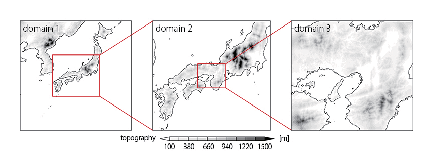
\includegraphics[width=1.0\hsize]{./figure/nesting_sample.eps}\\
  \caption{日本の近畿地方を対象領域とした領域ネスティング設定の例. domain 1が最外領域でdomain 3が最内領域である。
           赤い矩形と線は、それぞれの位置関係を示している。domain 1の水平格子間隔は7.5 km、domain 2は2.5 km、
           そしてdomain 3は0.5 kmである。}
  \label{fig_nestsample}
\end{center}
\end{figure}


\subsection{オフライン・ネスティング実験の方法} \label{sec:nest_offline}
%------------------------------------------------------

ここでは、
親領域は解像度は粗いが広領域の外側領域で、子領域は領域は狭いが高解像度の内側領域で
あるとする。このとき、2段ネスティングのオフライン・ネスティング実験の実行過程は次のようになる。

{\gt
\begin{enumerate}
 \item 親領域の時間積分計算を行う。
 \item 親領域の出力ファイル(history)を用いて子領域の初期値/境界値を作成する。
 \item 作成した初期値/境界値を用いて子領域の時間積分計算を行う。
\end{enumerate}
}

以下、この流れに沿って説明を進める。親領域と子領域それぞれについて、``pp.***.conf''、``init.***.conf''、
そして``run.***.conf''ファイルを事前に作成し、親領域、子領域ともに地形/土地利用データの作成を終え、
親領域については、初期値/境界値データの作成を終えていることを想定して説明を進める。
ここで説明するオフライン・ネスティング実験の設定を記述した設定ファイルがチュートリアルディレクトリの下、
``tutorial/real/sample/offline\_nesting''に置いてあるので、説明を読み進める上で参考にしてもらいたい。

\subsubsection{親領域の時間積分計算を行う}
基本的には通常のシングル領域の計算と同じ方法で実行すればよいが、``run.conf''ファイルの設定について、
次の5点に注意して設定する必要がある。

\begin{itemize}
 \item 親領域のhistory出力間隔を適度に細かくとること。
 \item 親領域のhistory出力変数に必要なものが揃っているか確認すること。
 \item 親領域のhistory出力形式で\verb|ZINTERP|は``false''に設定すること。
 \item 親領域のhistory出力形式で\verb|STEP0|は``true''に設定すること。
 \item 親領域の計算領域を子領域へ伝える「カタログファイル」を出力すること。
\end{itemize}


この設定を``run.parent.conf''に適用すると下記のようになる。赤文字で示した部分が、
上記の注意点・変更点に対応する部分である。\\

\noindent {\small {\gt
\ovalbox{
\begin{tabularx}{140mm}{l}
\textcolor{red}{\verb|&PARAM_DOMAIN_CATALOGUE|} \\
\textcolor{red}{\verb| DOMAIN_CATALOGUE_OUTPUT = .true.,|} \\
\textcolor{red}{\verb|/|} \\
 \\
\verb|&PARAM_HISTORY| \\
\verb| HISTORY_DEFAULT_BASENAME  = "history",| \\
\textcolor{red}{\verb| HISTORY_DEFAULT_TINTERVAL = 600.D0,|} \\
\verb| HISTORY_DEFAULT_TUNIT     = "SEC",| \\
\verb| HISTORY_DEFAULT_TAVERAGE  = .false.,| \\
\verb| HISTORY_DEFAULT_DATATYPE  = "REAL4",| \\
\textcolor{red}{\verb| HISTORY_DEFAULT_ZINTERP   = .false.,|} \\
\textcolor{red}{\verb| HISTORY_OUTPUT_STEP0      = .true.,|} \\
\verb|/| \\
\end{tabularx}
}}}\\

\verb|PARAM_DOMAIN_CATALOGUE|の項目の``\verb|DOMAIN_CATALOGUE_OUTPUT|''の変数がカタログファイルの出力設定である。
もともとの設定ファイルには項目自体がないこともあるので、その場合は自分で項目を加えて設定すること。
カタログファイルは、``latlon\_domain\_catalogue.txt''というファイル名で出力される。この中には、MPIプロセス毎に分割
して担当した計算領域の四隅の緯度・経度が記述されている。

\verb|HISTORY_DEFAULT_TINTERVAL|の設定項目によってhistoryデータ出力間隔を指定する(単位は秒である)。指定値に
任意性はあるが、子領域の側面境界条件の更新間隔として使用可能であると考えられる範囲で指定すること。
メソ気象の計算では、おおよそ最大で1時間間隔、10分間隔のhistoryデータ出力間隔を指定することが多い。
実行環境のディスク空き容量に注意されたい。


また、historyデータを用いて初期値/境界値データを作成するために、
下記の全ての変数を出力する必要がある。
run.confファイルの``HISTITEM''の項目を確認すること。

\begin{itemize}
 \item \verb|T2, Q2, MSLP, DENS, MOMZ, MOMX, MOMY, RHOT|
 \item \verb|QV, QC, QR, QI, QS, QG| {\small (親の雲微物理モデルに合わせて出力; 例えばTomita08なら全て)}
 \item \verb|NC, NR, NI, NS, NG| {\small (親の雲微物理モデルに合わせて出力; 例えばTomita08なら不要)}
 \item \verb|LAND_SFC_TEMP, URBAN_SFC_TEMP, OCEAN_SFC_TEMP|
 \item \verb|OCEAN_ALB_LW, OCEAN_ALB_SW, LAND_ALB_LW, LAND_ALB_SW|
 \item \verb|OCEAN_TEMP, OCEAN_SFC_Z0M, LAND_TEMP, LAND_WATER|
\end{itemize}

設定が完了すれば、scale-rmを実行して親領域の時間積分計算を行う。


\subsubsection{親領域の出力ファイルを用いて子領域の初期値/境界値を作成する}
次に計算が終わった親領域のhistoryデータ出力を用いて、子領域の初期値/境界値を作成する。
実行するプログラムは、通常の初期値/境界値作成と同じ``scale-rm\_init''だが、
``init.child.conf''を下記のように編集する。\\

\noindent {\small {\gt
\ovalbox{
\begin{tabularx}{140mm}{l}
\verb|&PARAM_MKINIT_REAL| \\
\verb| BASENAME_BOUNDARY   = "boundary",| \\
\textcolor{red}{\verb| BASENAME_ORG        = "history",|} \\
\textcolor{red}{\verb| FILETYPE_ORG        = "SCALE-RM",|} \\
\textcolor{red}{\verb| NUMBER_OF_TSTEPS    = 25,|} \\
\textcolor{red}{\verb| BOUNDARY_UPDATE_DT  = 600.D0,|} \\
\verb|/| \\
 \\
\textcolor{red}{\verb|&PARAM_NEST|} \\
\textcolor{red}{\verb| USE_NESTING               = .true.,|} \\
\textcolor{red}{\verb| OFFLINE                   = .true.,|} \\
\textcolor{red}{\verb| OFFLINE_PARENT_PRC_NUM_X  = 4,|} \\
\textcolor{red}{\verb| OFFLINE_PARENT_PRC_NUM_Y  = 4,|} \\
\textcolor{red}{\verb| OFFLINE_PARENT_KMAX       = 35,|} \\
\textcolor{red}{\verb| OFFLINE_PARENT_IMAX       = 40,|} \\
\textcolor{red}{\verb| OFFLINE_PARENT_JMAX       = 40,|} \\
\textcolor{red}{\verb| OFFLINE_PARENT_LKMAX      = 5,|} \\
\textcolor{red}{\verb| LATLON_CATALOGUE_FNAME    = "latlon_domain_catalogue.txt",|} \\
\textcolor{red}{\verb|/|} \\
\end{tabularx}
}}}\\

\noindent 読み込む外部入力データのファイル名を指定する``\verb|BASENAME_ORG|''は、親モデルのhistory.pe***.nc
ファイルを読み込むので、``history''と指定する。また、このhistoryファイルはSCALE-RMモデルの出力データなので、
``\verb|FILETYPE_ORG|''は、``SCALE-RM''と指定する。\verb|NUMBER_OF_TSTEPS|には、historyファイルが持つ時間ステップ数
を記述する(例として25が記述されているだけ)。\verb|BOUNDARY_UPDATE_DT|には、時間ステップの時間間隔を指定する
(単位は秒である)。つまり、親領域の\verb|HISTORY_DEFAULT_TINTERVAL|の設定項目に一致する値を指定する。
この説明では、親領域で600秒としたので、ここでも600秒を指定する。

\verb|PARAM_NEST|の項目は、ネスティング実験のために新たに加える項目である。もともとの設定ファイルには項目自体がないので、
自分で設定ファイルに追記する。最初の2つの項目によって、オフライン・ネスティング実験であることが決定される。
``\verb|OFFLINE_PARENT_|''で始まる6つの設定変数は、親領域の設定を記述する変数である。親領域の対応する項目を
参照して正しく設定すること。この例では、親領域は$4 \times 4$のMPIプロセス数を使用し、鉛直35層で、水平には1つの
MPIプロセスあたり$40 \times 40$の格子点を持っており、陸面モデルは5層モデルであることを想定している。
最後の``\verb|LATLON_CATALOGUE_FNAME|''の項目は、親領域を実行した時に出力したカタログファイルを指定する。

設定の編集が完了すれば、``scale-rm\_init''を実行して子領域の初期値/境界値を作成する。\\

\noindent {\small {\gt
\fbox{
\begin{tabularx}{140mm}{l}
\verb|xxx ERROR: REQUESTED DOMAIN IS TOO MUCH BROAD| \\
\verb|xxx -- LONGITUDINAL direction over the limit| \\
\end{tabularx}
}}}\\

\noindent 実行時に上記のようなメッセージが表示されて計算が止まる場合は、子領域の計算領域が親領域の計算領域の
外側に取られている部分がある。この場合は、各領域の大きさや領域中心の設定を見直す必要がある。


\subsubsection{作成した初期値/境界値を用いて子領域の時間積分計算を行う}
初期値/境界値作成が終われば、子領域の時間積分計算を実行する。子領域の実行は、通常の現実大気実験と何も変わらないので、
必要なデータのPATHが正しく設定ファイルに記述されていることを確認してから、``scale-rm''を実行すればよい。

1点だけ忘れやすい設定項目を挙げておく。\\

\noindent {\small {\gt
\ovalbox{
\begin{tabularx}{140mm}{l}
\verb|&PARAM_MKINIT_REAL| \\
\verb|     〜 中略 〜|\\
\textcolor{red}{\verb| BOUNDARY_UPDATE_DT  = 600.D0,|} \\
\verb|/| \\
\end{tabularx}
}}}\\

\noindent ``run.child.conf''の\verb|BOUNDARY_UPDATE_DT|を、初期値/境界値作成で使用した親領域の
historyデータ出力間隔に合わせておくことを忘れないようにすること。オフライン・ネスティング実験の場合、
現在のところこの設定に親領域と子領域間で不整合あっても警告やエラーメッセージが発せられないまま、
時間積分計算が進み、場合によっては正常終了してしまうため注意が必要である。

多段のオフライン・ネスティング実験を行いたい場合は、ここまでの過程を繰り返せばよい。つまり、子領域として
時間積分計算した結果を再度、親領域と見立てて、さらに内側の孫領域の初期値/境界値作成を行なえばよい。
以上でオフライン・ネスティングの実行方法の説明を終える。


\subsection{オンライン・ネスティング実験の方法} \label{sec:nest_online}
%------------------------------------------------------

オフライン・ネスティング実験では、各領域の計算を逐次的に実行する必要があったが、オンライン・ネスティング実験では
全ての領域の計算を同時に実行する。現在は、親領域から子領域へのみデータ受け渡しを行う、いわゆる
``1-wayネスティング''のみをサポートしている。オンライン・ネスティング実験でサポートするネスティング段数は、
最大で10段までである。

SCALEのオンライン・ネスティング実験は、複数の領域を逐次的に時間積分計算を進めるのではなく、並列的に時間積分計算を行う。
図\ref{fig_mpisplit}に示すイメージ図のように、与えられたMPIプロセスを分割してそれぞれの領域に分配し、各々の領域が
独立したモデルのように計算を進める。後ほど説明するが、複数の領域を立ち上げるために実行時には``launch.conf''という
起動用の設定ファイルが別途必要になる。

\begin{figure}[t]
\begin{center}
  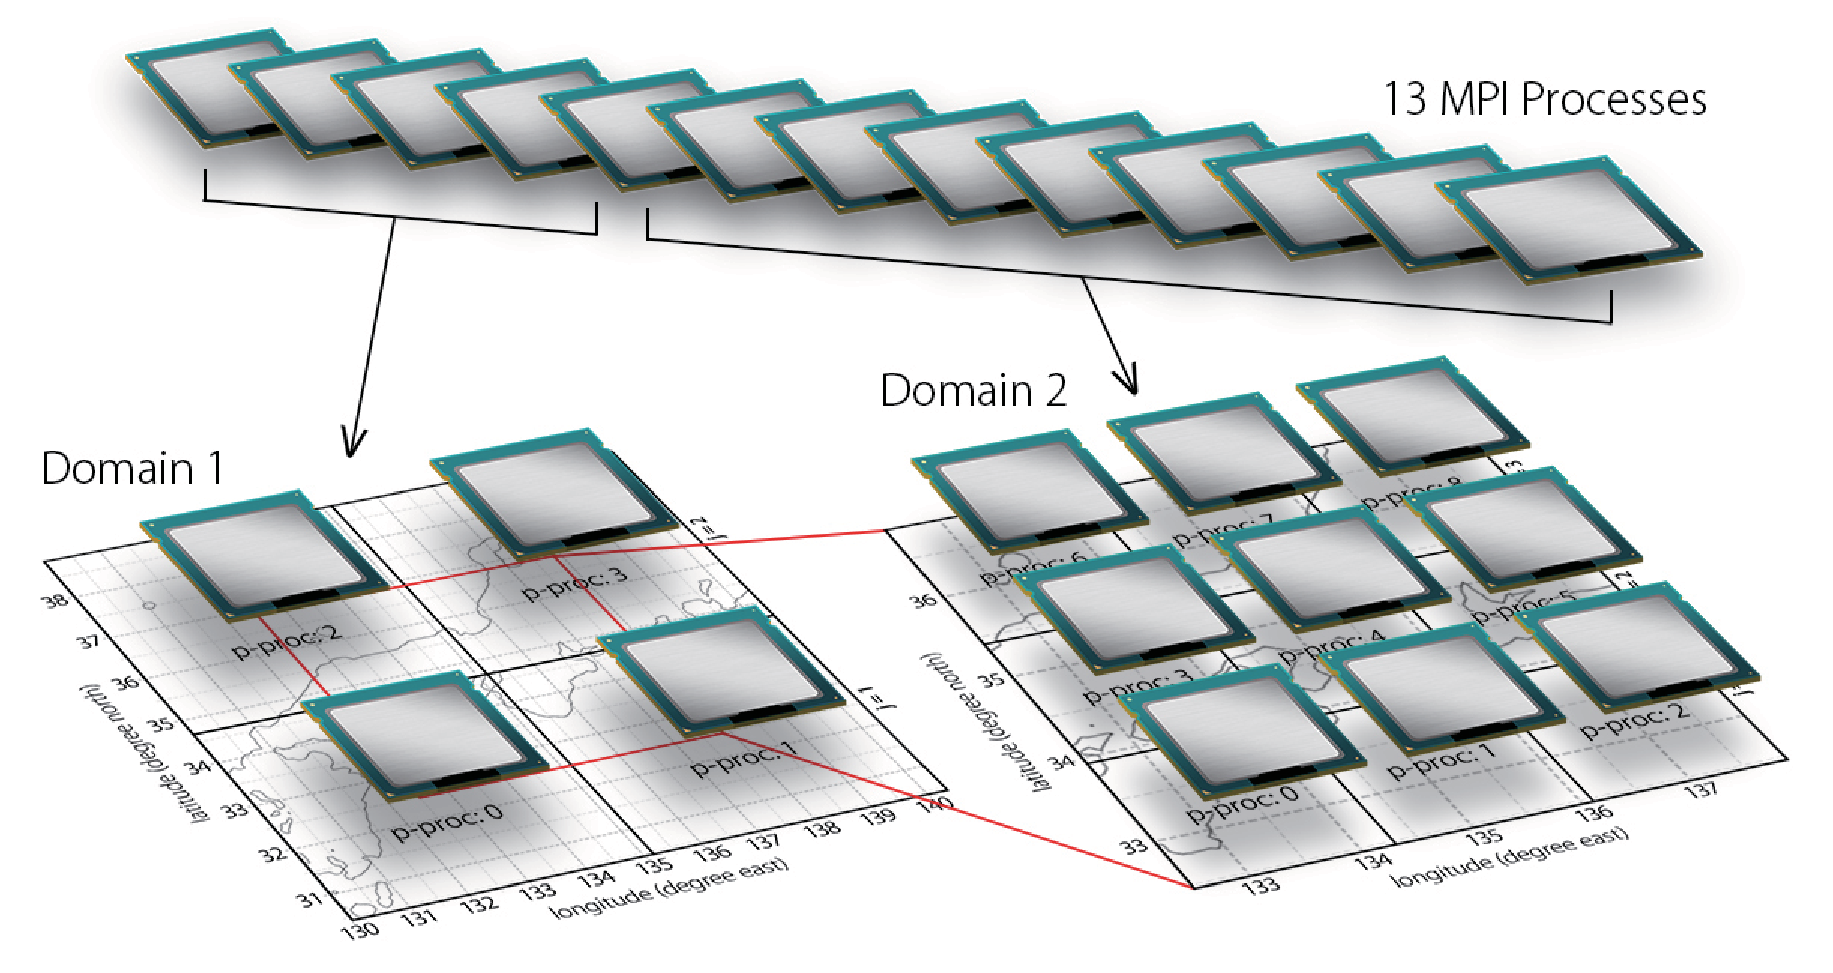
\includegraphics[width=0.8\hsize]{./figure/mpisplit_nesting.eps}\\
  \caption{オンライン・ネスティング実験のMPIプロセス配分イメージ. 全部で13のプロセスを立ち上げ、これを適切に分配することで、
           Domain 1は$2 \times 2$の4-MPI並列、Domain 2は$3 \times 3$の9-MPI並列計算を行う。Domain 1からDomain 2へMPI通信
           によってデータを受け渡ししながら時間積分計算を進める。}
  \label{fig_mpisplit}
\end{center}
\end{figure}


ここでは、最も単純な2段ネスティングの例を説明する。親領域は解像度は粗いが広領域の外側領域で、
子領域は領域は狭いが高解像度の内側領域であることを想定する。

オンライン・ネスティング実験を行う場合は、``scale-rm''のモデル本体実行前に全ての領域について、
地形/土地利用データの作成、及び初期値/境界値データの作成を事前に行っておく必要がある。従って、親領域と子領域
それぞれについて、``pp.***.conf''、``init.***.conf''、そして``run.***.conf''ファイルを事前に作成し、
親領域、子領域ともに地形/土地利用データの作成、及び初期値/境界値データの作成を終えていることを想定して説明を進める。
ここで説明するオンライン・ネスティング実験の設定を記述した設定ファイルがチュートリアルディレクトリの下、
``tutorial/real/sample/online\_nesting''に置いてあるので、説明を読み進める上で参考にしてもらいたい。


\subsubsection{設定ファイルの編集}
まず、親領域、子領域それぞれに``run.***.conf''ファイルを編集する。

\noindent {\gt \verb|run.parent.conf|の編集内容}\\
{\small {\gt
\ovalbox{
\begin{tabularx}{140mm}{l}
\verb|&PARAM_NEST| \\
\verb| USE_NESTING              = .true.,| \\
\verb| OFFLINE                  = .false.,| \\
\verb| ONLINE_DOMAIN_NUM        = 1,| \\
\verb| ONLINE_IAM_PARENT        = .true.,| \\
\verb| ONLINE_IAM_DAUGHTER      = .false.,| \\
\verb| ONLINE_BOUNDARY_USE_QHYD = .true.,| \\
\verb| ONLINE_AGGRESSIVE_COMM   = .true.,| \\
\verb|/| \\
\end{tabularx}
}}}\\

\vspace{0.5cm}

\noindent {\gt \verb|run.child.conf|の編集内容}\\
{\small {\gt
\ovalbox{
\begin{tabularx}{140mm}{l}
\verb|&PARAM_NEST| \\
\verb| USE_NESTING              = .true.,| \\
\verb| OFFLINE                  = .false.,| \\
\verb| ONLINE_DOMAIN_NUM        = 2,| \\
\verb| ONLINE_IAM_PARENT        = .false.,| \\
\verb| ONLINE_IAM_DAUGHTER      = .true.,| \\
\verb| ONLINE_BOUNDARY_USE_QHYD = .true.,| \\
\verb| ONLINE_AGGRESSIVE_COMM   = .true.,| \\
\verb|/| \\
\end{tabularx}
}}}\\

\noindent 上記の\verb|PARAM_NEST|の項目は、ネスティング実験のために新たに加える項目である。
もともとの設定ファイルには項目自体がないので、自分で設定ファイルに追記する。最初の2つの項目によって、
オンライン・ネスティング実験であることが決定される。``\verb| ONLINE_|''で始まる設定変数はオンライン・ネスティング実験
専用の設定変数である。\verb|ONLINE_DOMAIN_NUM|は、領域のID番号であり、外側領域から内側領域へ順番に
番号を振っていく。ここでは、親領域は1番、子領域は2番と設定する。

\verb|ONLINE_IAM_PARENT|と\verb|ONLINE_IAM_DAUGHTER|は各領域の役割を設定するパラメータである。
これらの変数は、``In online nesting system, I am parent (or, I am child).''という意味で覚えれば設定を間違うことはない。
少し脇道にそれるが、ここで説明している設定より複雑なものとして、図\ref{fig_nestsample}のような
3段ネスティング実験の場合の設定例を表\ref{tab:triple_nested}に示した。

\begin{table}[htb]
\begin{center}
\caption{3段ネスティング実験の設定例}
\begin{tabularx}{150mm}{|l|l|l|X|} \hline
 \rowcolor[gray]{0.9} 領域 & \verb|ONLINE_DOMAIN_NUM| & \verb|ONLINE_IAM_PARENT| & \verb|ONLINE_IAM_CHILD|\\ \hline
 最外領域 & 1 & \textcolor{blue}{true} & \textcolor{red}{false} \\ \hline
 中間領域 & 2 & \textcolor{blue}{true} & \textcolor{blue}{true} \\ \hline
 最内領域 & 3 & \textcolor{red}{false} & \textcolor{blue}{true} \\ \hline
\end{tabularx}
\label{tab:triple_nested}
\end{center}
\end{table}

\noindent 最外領域は親領域としてのみ働き、最内領域は子領域としてのみ働く。一方、中間領域は最外領域に
対しては子領域、最内領域に対しては親領域として働くため両方共``true''となる。

さて、設定ファイルの編集内容の説明に戻る。\verb|ONLINE_BOUNDARY_USE_QHYD|は、「側面境界条件として親領域の凝結物の
混合比を使うかどうか」を指定する設定変数である。外部入力データから側面境界条件を作成するときには通常使わないが、
ネスティングの場合、領域間の物理スキームの違いがなかったり、解像度もそれほど大きく離れていないため、側面境界から
凝結物自体が移流して入ってくる設定も選択肢に入るだろう。側面境界付近で雲が立ちにくい問題を解決したり、親領域との乖離を
抑制したりする可能性がある。

%最後の\verb|ONLINE_AGGRESSIVE_COMM|はオンライン・ネスティング時の領域間通信に関する最適化変数である。
%通常は、``true''と設定して実行する。


\subsubsection{launchファイルの編集}
オンライン・ネスティング実験の実行には、``run.***.conf''の他に、起動用設定ファイル``launch.conf''が必要である。
\begin{verbatim}
 $ vi launch.conf
\end{verbatim}
などとして、適宜エディタをたちあげて新規ファイルを作成し、下記の内容を記述する。\\

\noindent {\small {\gt
\ovalbox{
\begin{tabularx}{140mm}{l}
\verb|&PARAM_LAUNCHER| \\
\verb| NUM_DOMAIN  = 2,| \\
\verb| CONF_FILES  = run.parent.conf,run.child.conf,| \\
\verb| PRC_DOMAINS = 4,9,| \\
\verb|/| \\
\end{tabularx}
}}}\\

\noindent 図\ref{fig_mpisplit}のイメージを思い浮かべながら設定を確認してもらいたい。\verb|PARAM_LAUNCHER|の項目のうち、
\verb|NUM_DOMAIN = 2|が「2つの領域を起動する」ことを表しており、\verb|CONF_FILES|の項目に羅列されたファイル名は、
各々の領域で読み込む設定ファイルを指定している。\verb|PRC_DOMAINS|は各々の領域で使用するMPIプロセス数を
指定する。\verb|PRC_DOMAINS|は、\verb|CONF_FILES|で羅列した順番で指定しなければならない。従ってこの場合、
親領域は4-MPI並列、子領域は9-MPI並列で実行するように指定されている。ここで指定するMPIプロセス数は、
各々の``run.***.conf''で指定されている総MPIプロセス数と合致させなければならない。
この2段オンライン・ネスティング実験で使用する総MPIプロセス数は、$4 + 9 = 13$プロセスとなる。

実行時には、シングル領域計算とは異なり、\verb|launch.conf|を引数に指定し、計算全体で使用するMPIプロセス数を
指定して実行する。
\begin{verbatim}
 $ mpirun  -n  13  ./scale-rm  launch.conf
\end{verbatim}

実行にあたって注意することは、複数の領域の計算を同時に実行するため、\textcolor{red}{領域間で設定ファイルに
記述された出力ファイル名を領域毎に変更しなければならない}ことである。たとえば,``history.pe***.nc''は、
``history\_d01.pe***.nc''、``history\_d02.pe***.nc''といったように領域毎に名前を変えながらどの領域の
出力データであるか判別がつくように設定ファイルの記述を設定する。
historyファイルのほかに、LOGファイル、topoファイル、landuseファイル、boundaryファイル、initファイル、restartファイル、
そしてmonitorファイルの名前を変更しておく必要がある。

実行時に次のようなエラーメッセージが出力されて計算が異常終了することがある。\\

\noindent {\small {\gt
\fbox{
\begin{tabularx}{140mm}{l}
\verb|xxx region of daughter domain is larger than that of parent: SW search| \\
\end{tabularx}
}}}\\

\noindent {\small {\gt
\fbox{
\begin{tabularx}{140mm}{l}
\verb|xxx region of daughter domain is larger than that of parent: NE search| \\
\end{tabularx}
}}}\\

\noindent これは、子領域で設定された計算領域が親領域の計算領域よりも大きいことを意味するエラーメッセージである。
``SW search''のエラーが出る場合は子領域の西側か南側が親領域の外側に出ており、``NE search''のエラーが出る場合は
子領域の東側か北側が親領域の外側に出ていることを意味している。再度設定を確認し、地形・土地利用データ、および
初期値/境界値作成からやり直すこと。


\subsubsection{MPIプロセスの分配ガイドライン}
SCALEのオンライン・ネスティング実験は、図\ref{fig_mpisplit}のイメージ図で説明したように、MPIプロセスを分割し、複数の領域
に分配する。現在のところ、その分配割合はユーザーに委ねられているため、適切にMPIプロセスを分配しなければ余計な計算時間が
かかってしまう。ここでは、適切にMPIプロセスを分配するためのガイドラインについて説明する。ガイドラインは、領域毎に
\textcolor{blue}{「単位あたりの時間積分にかかる1プロセスあたりの演算量を揃える」}という単純なものである。
ここでは、以下に示す2段オンライン・ネスティング実験を行う場合を想定し、ガイドラインに沿ったプロセス分配方法の例を示す。
``domain 1''は外側の親領域、``domain 2''は内側の子領域を意味する。

\begin{table}[htb]
\begin{center}
\caption{2段オンライン・ネスティング実験の設定想定}
\begin{tabularx}{150mm}{|l|l|X|} \hline
 \rowcolor[gray]{0.9} 設定項目 & domain 1 & domain 2 \\ \hline
 計算領域 & 450 km $\times$ 450 km & 200 km $\times$ 200 km \\ \hline
 DX \& DY(X,Y同一設定) & 3 km & 1 km \\ \hline
 鉛直層設定 & 40層 & 60層 \\ \hline
 積分時間間隔(DT)& 30 sec & 10 sec \\ \hline
 積分時間 & 3600 sec & 3600 sec \\ \hline
\end{tabularx}
\label{tab:nest_proc_guide1}
\end{center}
\end{table}

このとき、親領域の水平方向の一辺の格子点数は、$450 \mathrm{km} \div 3 \mathrm{km} = 150$点であるので、総格子点数は
$X \times Y \times Z = 150 \times 150 \times 40 = 900,000$点である。一方、子領域の水平方向の一辺の格子点数は、
$200 km \div 1 km = 200$点であるので、総格子点数は$200 \times 200 \times 60 = 2,400,000$点である。1つの時間ステップの
積分を行うのにこれだけの格子点について計算を行わなければならない。

積分時間間隔は格子間隔に依存するために領域毎に異なる。この例では、domain 1は30 secだが、domain 2は10 secであり、
3倍の差がある。したがって、同じ30 secという積分時間に対してdomain 2は3倍多くの時間ステップ、つまり3倍の演算量を要する。
これらを考慮して、簡単な領域間の演算量比率(Computation Rate)の指標を考えると下記の式で表される。
\begin{eqnarray}
ComputationRate=\frac{Xgrd_{child} \times Ygrd_{child} \times Zgrd_{child} \times Ustep_{child}}
                     {Xgrd_{parent} \times Ygrd_{parent} \times Zgrd_{parent} \times Ustep_{parent}} \nonumber
\end{eqnarray}
ここで、$Xgrd, Ygrd, Zgrd$ はそれぞれ{\XDIR} 、{\YDIR}、{\ZDIR}の格子点数を表し、Ustepは単位時間積分に必要な時間ステップ数を表す。
ここでの例をこの式に当てはまると、演算量比率は$(2,400,000 \times 3) \div (900,000 \times 1) = 8$であることがわかる。
おおよそ、この割合にしたがってMPIプロセスを領域毎に分配すればよい。例えばdomain 1は4プロセス、domain 2は32プロセスを
使用し、全体で36プロセスを使用する設定が考えられる。この場合、例えば次のように設定することができる。

\begin{table}[htb]
\begin{center}
\caption{2段オンライン・ネスティング実験のMPIプロセス設定例}
\begin{tabularx}{150mm}{|l|l|X|} \hline
 \rowcolor[gray]{0.9} 設定項目 & domain 1 & domain 2 \\ \hline
 MPIプロセス(X $\times$ Y) & 2 $\times$ 2 & 4 $\times$ 8 \\ \hline
 水平格子点数(IMAX $\times$ JMAX) & 75 $\times$ 75 & 50 $\times$ 25 \\ \hline
\end{tabularx}
\label{tab:nest_proc_guide2}
\end{center}
\end{table}

{\XDIR} と{\YDIR}に分配するプロセス数には任意性が残るが、
IMAXとJMAXの違を小さくとる方がHalo領域を小くすることが出来るため、計算機の演算性能を引き出しやすいと考えられる\footnote{ただし、京の場合のようにスレッド並列も併用するハイブリッド並列の場合には{\YDIR}の格子点数をある程度大きくしてスレッド間の演算量のインバランスを小さくする必要性も出てくる。}。

この設定は一例であり、これ以外の方法で設定しても構わない。また、ここでは格子点数と積分時間間隔だけに着目して演算量比率
を考えたが、実際の計算には様々な物理過程も含まれるだろうし、それらを 呼び出す時間間隔も領域毎に異なるかもしれない。
さらに領域内通信や領域間通信のMPI通信にかかる時間も影響を及ぼす。
オンライン・ネスティングの設定では、最も計算負荷が高い領域(通常は最内領域)が時間積分を実行し続ける(MPI通信のための待ち時間が最小になる)ようにプロセスを分配するのが効率的である場合が多い。
同じ設定で何度も実験を行うような場合には、上記の方法である程度の見通しをつけた上で、いくらかの微調整を行うことをおすすめする。
以上でオンライン・ネスティングの実行方法の説明を終える。


\subsection{子領域における地形の取り扱い} \label{sec:nest_topo}
%------------------------------------------------------
ネスティング実験を行う際、領域間の格子間隔比率が大きい場合などに
子領域の緩和領域内で不整合が発生する
可能性がある。
緩和領域内は親領域の計算結果を用いて一部の変数を緩和していくが、地形の表現性が異なる
ことで、子領域にとっては正しくない値へ引きずられる可能性がある。
例えば、子領域では斜面上の小さな谷として
表現されている地形が、親領域では格子間隔が大きすぎて
谷がなくスムーズな斜面として表現される場合が考えられる。

こういった不整合を無くすために、緩和領域では親領域の地形を用い、内側領域では子領域自身の地形を用いる
「地形コピー」の機能が実装されている。この機能を使えば、図\ref{fig_topocopy}に示すように緩和領域は完全に
親領域に一致する地形で、内側に移る地形遷移領域内では親領域と子領域のミックス、それより内側では完全に
子領域の地形という設定を構築することができる。以降、その設定方法と実行手順を説明する。基本的には、
オフライン・ネスティングのフレームワークを利用して進める。
ここで説明する地形コピーの設定を記述した``pp.d0*.conf''ファイルがチュートリアルディレクトリの下、
``tutorial/real/sample/online\_nesting''に置いてあるので、説明を読み進める上で参考にしてもらいたい。

\begin{figure}[tb]
\begin{center}
  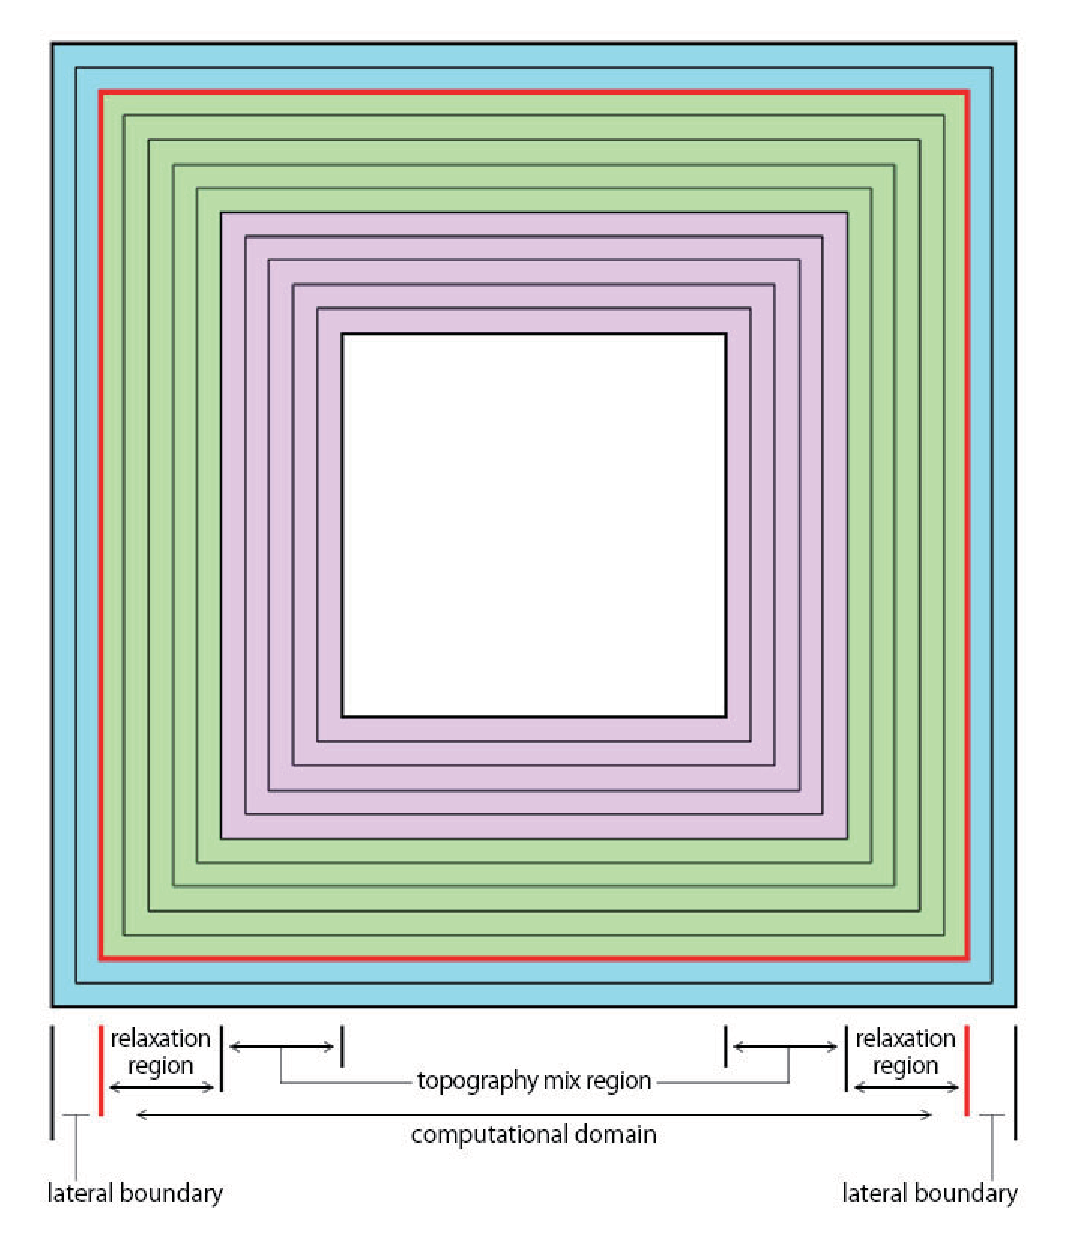
\includegraphics[width=0.4\hsize]{./figure/topo_copy.eps}\\
  \caption{地形コピーを適用した子領域の地形データ水平分布. 最外の水色の2格子(Haloの数。水平差分スキームによって異る)は側面境界で、それより内側の赤色の線で
           囲われた領域が計算領域である。緑色の部分が緩和領域、桃色の部分が地形遷移領域、そして最内の白色の
           部分が子領域の地形をもつ領域である。地形遷移領域では外側から内側にかけて徐々に親領域の地形データから
           子領域の地形データへ遷移する。}
  \label{fig_topocopy}
\end{center}
\end{figure}

まず親領域の``pp.d01.conf''ファイルを編集して、計算領域の大きさを子領域へ伝えるために緯度経度カタログ
ファイルを出力するように設定する。具体的には、下記の記述を``pp.d01.conf''ファイルに追記する。\\

\noindent {\small {\gt
\ovalbox{
\begin{tabularx}{140mm}{l}
\verb|&PARAM_DOMAIN_CATALOGUE| \\
\verb| DOMAIN_CATALOGUE_FNAME  = "latlon_domain_catalogue.txt",| \\
\verb| DOMAIN_CATALOGUE_OUTPUT = .true.,| \\
\verb|/| \\
\end{tabularx}
}}}\\

\noindent その他の設定項目は通常通りで良い。編集ができたら親領域の地形データ作成を実行する(つまり、
scale-rm\_ppを実行する)。ここで、出力データは、``topo\_d01.pe***.nc''というファイル名で保存されていると
想定する。次に、子領域の``pp.d02.conf''ファイルを編集する。\\

\noindent {\small {\gt
\ovalbox{
\begin{tabularx}{140mm}{l}
\verb|&PARAM_CNVTOPO| \\
\verb|     〜 中略 〜|\\
\verb| CNVTOPO_copy_parent     = .true.,| \\
\verb|/| \\
 \\
\verb|&PARAM_COPYTOPO| \\
\verb| COPYTOPO_IN_BASENAME   = "topo_d01",| \\
\verb| COPYTOPO_ENTIRE_REGION = .false.,| \\
\verb| COPYTOPO_LINEAR_H      = .true.,| \\
\verb|/| \\
 \\
\verb|&PARAM_NEST| \\
\verb| USE_NESTING               = .true.,| \\
\verb| OFFLINE                   = .true.,| \\
\verb| OFFLINE_PARENT_PRC_NUM_X  = 4,| \\
\verb| OFFLINE_PARENT_PRC_NUM_Y  = 4,| \\
\verb| OFFLINE_PARENT_KMAX       = 35,| \\
\verb| OFFLINE_PARENT_IMAX       = 40,| \\
\verb| OFFLINE_PARENT_JMAX       = 40,| \\
\verb| OFFLINE_PARENT_LKMAX      = 5,| \\
\verb| LATLON_CATALOGUE_FNAME    = "latlon_domain_catalogue.txt",| \\
\verb|/| \\
\end{tabularx}
}}}\\

\noindent もともと設定ファイルにある\verb|PARAM_CNVTOPO|の項目に、\verb|CNVTOPO_copy_parent = .true.|
という記述を加える。これは地形コピーの実行を指示するスイッチである。
次の\verb|PARAM_COPYTOPO|は、地形コピーの設定項目群であり、すべて追記すること。
1つ目の\verb|COPYTOPO_IN_BASENAME|は、親領域の地形データのPATHを指定する。ここでは、親領域の
出力データは``topo\_d01.pe***.nc''というファイル名でカレントディレクトリに保存されていると指定している。
2つ目の\verb|COPYTOPO_ENTIRE_REGION|は、全領域でコピーするかどうかを決定するオプションである。
このスイッチをtrueにすると、図\ref{fig_topocopy}に示された桃色と白色の領域は無くなり、全て緑色の
完全コピー領域になる。3つ目の\verb|COPYTOPO_LINEAR_H|は、地形遷移領域の遷移具合を調整するスイッチである。
\verb|COPYTOPO_LINEAR_H|がtrueだと線形プロファイルで遷移し、falseだと指数関数プロファイルで遷移する。

地形遷移領域の幅は、デフォルト設定では緩和領域と同じ幅になる。緩和領域の設定と同じ要領で、
\verb|COPYTOPO_TRANSITION_DX|、\verb|COPYTOPO_TRANSITION_DY|、および\verb|COPYTOPO_TRANSFACT|の
変数を使って任意の幅に設定することができる。

最後の\verb|PARAM_NEST|の項目はオフライン・ネスティング実験のフレームワークを利用するための設定項目であり、
全て追記する必要がある。設定変数の詳しい説明は、\ref{sec:nest_offline}節のオフライン・ネスティング実験の説明を
参照してほしい。

設定ファイルの編集が終われば、子領域の地形データ作成を実行する。3つ以上の領域がある場合は、
上記の実行過程を外側領域から順に繰り返せばよい。




\section{\SecAdvanceBulkjob} \label{sec:bulkjob}
%====================================================================================

SCALE-RMには「一括実行機能」、いわゆるバルクジョブ機能が備わっている。これは、パラメタスイープ実験、
初期値アンサンブル実験や、タイムスライス気候実験など多数の実験を行う場合に便利な機能である。SCALE-RMモデル本体の実行は
もちろん、ドメインネスティング実験の場合でも利用できるし、地形・土地利用データ作成(地形コピーを利用しない場合のみ)、
初期値/境界値作成、そして後処理ツールのnet2g(netcdf2grads\_bulkを使用)にも適用可能である。
各プログラムの実行内容は異なっていても構わないが、MPI並列としての構造は共通していなければならない点に注意すること。
1つの計算事例をここでは「ジョブ」と呼ぶこととする。以下では、3つの2段オンライン・ネスティング実験を一括に行う例を
もとに説明する(積分期間、もしくは計算領域中心が異なっている3つのジョブを想定している)。


\begin{figure}[t]
\begin{center}
  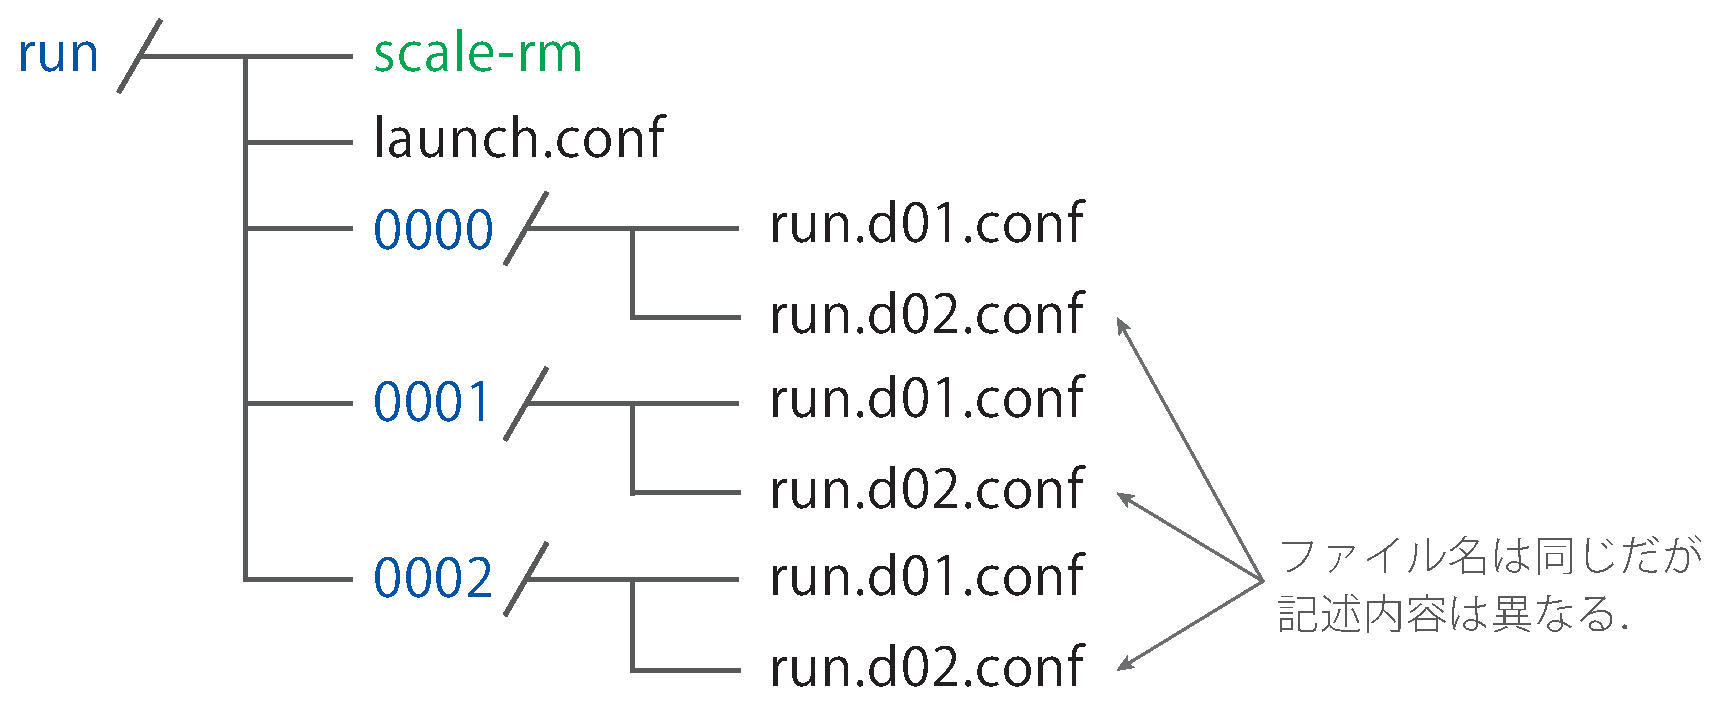
\includegraphics[width=0.6\hsize]{./figure/bulkjob_directory_structure.eps}\\
  \caption{バルクジョブ機能を使ってscale-rmを実行する場合のディレクトリ構造. ``0000''や``0001''はジョブ番号
           に対応する名前を持ったジョブディレクトリである。各ジョブディレクトリの中には、そこで実行する実験に関する
           設定ファイルが置かれている。データパラメタテーブルなどのファイルやディレクトリの記述は割愛しているが、
           それらも必要に応じて適切に配置する必要がある。}
  \label{fig_bulkjob}
\end{center}
\end{figure}


バルクジョブ実行するにあたって下記のものを事前に準備する必要がある。
\begin{itemize}
\item バルクジョブ用のディレクトリ構造
\item 実験に必要なすべての設定ファイル
\item 実験に必要なすべての外部入力データ
\end{itemize}

まず、図\ref{fig_bulkjob}に示すようなディレクトリ構造を準備する。``0000''や``0001''といったディレクトリは、
ジョブ番号に対応する名前を持ったジョブディレクトリである。ジョブディレクトリは必ず4桁の数字で、ジョブ番号はゼロから
数え上げられる。これらのディレクトリの中には設定ファイルが収められている。
今回は2段オンライン・ネスティング実験を想定しているので、``run.d01.conf''と``run.d02.conf''の2つのファイルが準備
されている。各ジョブディレクトリにある設定ファイルの名前は同じにする必要があるが、内容は異なっていても構わない。
ただし、\textcolor{red}{ドメイン毎に使用するMPIプロセス数は全てのジョブで共通していなければならない。}
設定ファイル内にバルクジョブ機能用に追加する設定項目はないが、\textcolor{red}{入出力ファイルのPATHを適切に
記述する}必要がある。以下にジョブ0000番のrun.d01.confの抜粋を示す。\\

\noindent {\small {\gt
\ovalbox{
\begin{tabularx}{140mm}{l}
\verb|&PARAM_IO| \\
\textcolor{blue}{\verb| IO_LOG_BASENAME = "0000/LOG_d01",|} \\
\verb|/| \\
 \\
\verb|&PARAM_RESTART| \\
\verb| RESTART_OUTPUT       = .true.,| \\
\textcolor{blue}{\verb| RESTART_OUT_BASENAME = "0000/restart_d01",|} \\
\textcolor{cyan}{\verb| RESTART_IN_BASENAME  = "../init/0000/init_d01_00013046400.000",|} \\
\verb|/| \\
 \\
\verb|&PARAM_TOPO| \\
\textcolor{cyan}{\verb| TOPO_IN_BASENAME = "../pp/0000/topo_d01",|} \\
\verb|/| \\
 \\
\verb|&PARAM_LANDUSE| \\
\textcolor{cyan}{\verb| LANDUSE_IN_BASENAME = "../pp/0000/landuse_d01",|} \\
\verb|/| \\
 \\
\verb|&PARAM_ATMOS_BOUNDARY| \\
\verb|     〜 中略 〜|\\
\textcolor{cyan}{\verb| ATMOS_BOUNDARY_IN_BASENAME    = "../init/0000/boundary_d01",|} \\
\verb|     〜 以下略 〜|\\
\verb|/| \\
 \\
\verb|&PARAM_HISTORY| \\
\textcolor{blue}{\verb| HISTORY_DEFAULT_BASENAME  = "0000/history_d01",|} \\
\verb|     〜 以下略 〜|\\
\verb|/| \\
\end{tabularx}
}}}\\

\noindent 上記の設定ファイルの設定例のうち、青色文字の部分は出力ファイルの指定、水色文字の部分は入力ファイルの指定である。
図\ref{fig_bulkjob}を見てわかるように、実行バイナリ(scale-rm)があるのは``runディレクトリ''の下で、
ジョブディレクトリも実行バイナリと同じ階層にある。従って、ジョブ0000番において、実行バイナリからみてデータを出力するべき
ディレクトリは、``0000/''の下である。そこで出力ファイル名の指定として``0000/***''と記述している。

入力ファイルについても同様である。ここでは、runディレクトリと同じ階層にppディレクトリやinitディレクトリがあり、
その中にまたジョブディレクトリが作成してあって、それらの中に入力ファイルが保管されている状況を想定している。
従って、runディレクトリの下で実行される実行バイナリにとっては、``../pp/0000/***''といったPATHになる。

バルクジョブ機能は、オンライン・ネスティング実験で利用したMPIプロセスを分割・分配する機能を使って実装されている。
したがって、ジョブの起動のために``launch.conf''ファイルが必要になる。オンライン・ネスティング実験とバルクジョブ機能を
併用して実行する今回のような場合もlaunch.confファイルは1つだけで良い。\\

\noindent {\small {\gt
\ovalbox{
\begin{tabularx}{140mm}{l}
\verb|&PARAM_LAUNCHER| \\
\verb| NUM_BULKJOB = 3,| \\
\verb| NUM_DOMAIN  = 2,| \\
\verb| PRC_DOMAINS = 9,36,| \\
\verb| CONF_FILES  = run.d01.conf,run.d02.conf,| \\
\verb|/| \\
\end{tabularx}
}}}\\

\noindent 上記がオンライン・ネスティング実験とバルクジョブ機能を併用して実行する場合のlaunch.confファイルの中身である。
オンライン・ネスティング実験の場合のlaunch.confファイルに対して、\nmitem{NUM_BULKJOB}の設定項目を加えただけとなっている。
ここで実行するジョブ数は3つであるので、\nmitem{NUM_BULKJOB}に対して``3''と指定する。シングルドメイン実験として
バルクジョブ機能を利用する場合は、\nmitem{NUM_DOMAIN = 1}と指定して、\nmitem{CONF_FILES}に1つだけ設定ファイルを指定すればよい。
実行時のコマンドは、

\begin{verbatim}
 $ mpirun  -n  135  ./scale-rm  launch.conf
\end{verbatim}

となる。ここでは1ジョブあたり、$9 + 36 = 45$プロセス使用し、全体で3つのジョブを実行するので、総計で135プロセスを
必要とする。

実行すると得られるLOGファイルに、MPIプロセスを分割した時の情報が示されている。LOGファイルを開いて最初の
「SCALEロゴ」のあとに下記のようなメッセージが出力される。\\

\noindent {\small {\gt
\ovalbox{
\begin{tabularx}{140mm}{l}
\verb| ++++++ Start MPI| \\
\verb| *** UNIVERSAL_COMM_WORLD        :        0| \\
\verb| *** total process [UNIVERSAL]   :      135| \\
\verb| *** my process ID [UNIVERSAL]   :       36| \\
\verb| *** master rank?  [UNIVERSAL]   :        F| \\
\verb| *** GLOBAL_COMM_WORLD           :        3| \\
\verb| *** total process [GLOBAL]      :       45| \\
\verb| *** my process ID [GLOBAL]      :       36| \\
\verb| *** master rank?  [GLOBAL]      :        F| \\
\verb| *** LOCAL_COMM_WORLD            :        4| \\
\verb| *** total process [LOCAL]       :        9| \\
\verb| *** my process ID [LOCAL]       :        0| \\
\verb| *** master rank?  [LOCAL]       :        T| \\
\verb| *** ABORT_COMM_WORLD            :        0| \\
\verb| *** master rank ID [each world] :        0| \\

\end{tabularx}
}}}\\

これらのうち、\verb|[LOCAL]|と表記されている項目はドメイン内のプロセスグループ、\verb|[GLOBAL]|と表記されている項目は
ネスティング・グループ、\verb|[UNIVERSAL]|と表記されて項目はジョブ・グループに関する情報である。
したがって、このLOGメッセージから、当該ドメインは12-MPI並列で実行されており、オンライン・ネスティング実験は総計で
48プロセス使用して実行され、バルクジョブ全体では1488プロセスが使用されているため、同時に31個のジョブが走っていたことがわかる。
異常終了したときにも、この表記法に従ってメッセージが出力されるので、これを理解しているとバルクジョブ機能を使って多量に
走らせている場合にも、どのプロセスがエラーを発生したのか即座に判断できる。ちなみに現在のバルクジョブ機能では、
1つのジョブがエラーを発生し、異常終了状態に入ると全てのジョブが異常終了する。



%%%%%%%%%%%%%%%%%%%%%%%%%%%%%%%%%%%%%%%%%%%%%%%%%%%%%%%%%%%%%%%%%%%%%%%%%%%%%%%%%%%%%%


\bibliographystyle{plainnat}
\bibliography{reference}

\begin{appendix}

\chapter{ライブラリ環境のインストール} \label{achap:env_setting}
%%%%%%%%%%%%%%%%%%%%%%%%%%%%%%%%%%%%%%%%%%%%%%%%%%%%%%%%%%%%%%%%%%%%%%%%%%%%%%%%%%%%%%%%%%%%

SCALEのインストールに必要なコンパイラやライブラリ環境のインストール方法について説明する。
ここでの記載内容は、こちらのテスト環境でのインストールプロセスを示しているものであって
必ずしも全く同じとは限らない。
うまくいかない場合には、それぞれのツール・ライブラリの開発元に直接問い合わせること。


Linuxをインストール後、各種プログラムのインストールはコマンドライン端末にて行う。
本書で説明するライブラリ環境のインストールでは、root権限が必要になる。
したがって、想定する環境は、ユーザーがroot権限を所持しているかサーバやデスクトップマシンである。
別途サーバー管理者が存在し、root権限を取得できない場合等は、必要な環境条件が整っているか
サーバー管理者に問い合わせること。

本節では、HDF5, NetCDF, MPIについてGNU compilerでコンパイルされたライブラリの説明を行う。
GNU compiler以外のIntel compilerなどを利用する場合は、各自でインストール方法を調べてインストールすること。\\

\noindent ここでインストールするコンパイラおよびライブラリ環境は、主に下記の4点である。
\begin{itemize}
\item GNU C/C++, fortran compiler
\item HDF5 Library (\url{https://www.hdfgroup.org/HDF5/})
\item NetCDF Library (\url{http://www.unidata.ucar.edu/software/netcdf/})
\item Message Passing Interface (MPI) Library (openMPI版、\url{http://www.open-mpi.org/})
\end{itemize}
これらのインストール方法について、本書では下記の5種類のOperating System (OS)について説明する。
\begin{itemize}
\item Linux CentOS 6.6 x86-64
\item Linux CentOS 7.1 x86-64
\item Linux openSUSE 13.2 x86-64
\item Apple Mac OS X 10.10 Yosemite
\item スーパーコンピュータ「京」
\end{itemize}
他のOSディストリビューション(下記参照)でもSCALEを利用可能だが、
本書でサポートするのは上記の範囲とする。\\

\noindent{\bf 動作確認済みの他のOSディストリビューション}
\begin{itemize}
\item Linux SUSE Enterprise Linux 11.1, 11.3 x86-64
\item Linux Vine Linux 6.3 x86-64
\item Linux Fedora 16 x86-64
\end{itemize}


\section{インストール方法 (Linux - CentOS 6.6-6.8 編)} \label{chap:install_centos}
%==========================================================================================

以下の説明で使用した環境は次のとおりである。
\begin{itemize}
\item CPU: Intel Core i5 2410M (sandybridge)
\item Memory: DDR3-1333 4GB
\item OS: CentOS 6.6 (kernel: 2.6.32-504.23.4.el6.x86\_64)\\
{\small *インストール時、"日本語"、 "Desktop"、"Kdump有り"を選択}
\end{itemize}

\subsubsection{ライブラリのインストール}

CentOS 6.6では、一部のライブラリをエンタープライズLinux用の拡張パッケージ(EPEL)リポジトリからインストールする。
そこで、はじめにEPELリポジトリをシステムにインストールし登録する。
CentOS 6.6では、ソフトウェアのインストールに"yum"コマンドを利用する。
すべての作業を行うまえに、下記のコマンドにてパッケージをアップデートしておくことをおすすめする。
\begin{verbatim}
 # yum update
\end{verbatim}

ルート権限で、下記のコマンドを実行することでリポジトリの登録が可能である。
\begin{verbatim}
 # yum install epel-release
\end{verbatim}
実行時のコマンドラインの様子は以下のようになる。
インストール対象がリストされるので、確認して"y"をタイプして先へ進める。\\

\noindent {\small {\gt
\fbox{
\begin{tabularx}{140mm}{l}
読み込んだプラグイン:fastestmirror, refresh-packagekit, security\\
インストール処理の設定をしています\\
Loading mirror speeds from cached hostfile\\
 * base: ftp.***.**.jp\\
 * extras: ftp.***.**.jp\\
 * updates: ftp.***.**.jp\\
依存性の解決をしています\\
-- トランザクションの確認を実行しています。\\
--- パッケージ epel-release.noarch 0:7-5 を インストール\\
-- 依存性解決を終了しました。\\
\\
依存性を解決しました\\
\\
======================================\\
 Package                アーキテクチャー バージョン      リポジトリー      容量\\
======================================\\
インストール中:\\
 epel-release           noarch           6-8             extras            14 k\\
\\
トランザクションの要約\\
======================================\\
インストール  1 パッケージ\\
\\
総ダウンロード容量: 14 k\\
インストール容量: 24 k\\
Is this ok (y/N): y\\
パッケージをダウンロードしています:
epel-release-6-8.noarch.rpm                                   14 kB     00:00\\
rpm\_check\_debug を実行しています\\
トランザクションのテストを実行しています\\
トランザクションのテストを成功しました\\
トランザクションを実行しています\\
  インストールしています  : epel-release-6-8.noarch                            1/1\\
  Verifying               : epel-release-6-8.noarch                            1/1\\
\\
インストール:\\
  epel-release.noarch 0:6-8\\
\\
完了しました!\\
\end{tabularx}
}}}\\

\noindent {\small *この時点で、yumによるインストールに失敗する場合は、
プロキシ設定等を含めた通信環境、yumリポジトリの登録状況等を再確認すること。}

\noindent yumのグループインストール機能を用いて,開発ツール
(ここでの対象は主にGNU compilerとmakeシステム)をまとめてインストールする。
\begin{verbatim}
 # yum groupinstall "development tools"
\end{verbatim}

\noindent つづいて、グループインストールではインストールされないライブラリを個別に追加する。
\begin{verbatim}
 # yum install zlib-devel
 # yum install hdf5-devel hdf5-static
 # yum install netcdf-devel netcdf-static
 # yum install openmpi-devel
 # yum install wgrib wgrib2
\end{verbatim}

SCALEは陰解法計算の部分で、数値計算ライブラリ Lapack
\footnote{\url{http://www.netlib.org/lapack/}}
を利用するオプションがある。
もし必要ならば、Lapack もインストールすること。
\begin{verbatim}
 # yum install lapack lapack-devel
\end{verbatim}

\noindent \textcolor{blue}{\small *wgrib、wgrib2は、第\ref{chap:tutorial_real}章:Tutorial: Real case で
外部入力データのプレ処理を行うために使用する。}

\noindent {\small *"yum -y install package name" のように ``-y'' オプションをつけて実行することで、インストール前の再確認をスキップできる。}


\subsubsection{環境変数の設定}

ローカルシステムでMPI並列プログラムを実行するために、OpenMPIライブラリの環境変数設定を行う。
ユーザ権限に移動して.bashrcをエディタで開き,
\begin{verbatim}
 $ vi ~/.bashrc
\end{verbatim}
下記をファイルの最後に追加して,環境変数の設定を記述する。\\

\noindent {\gt
\ovalbox{
\begin{tabularx}{140mm}{l}
 \\
 \verb|// ---------------- Add to end of the file ----------------|\\
 \verb|# OpenMPI|\\
 \verb|export MPI="/usr/lib64/openmpi"|\\
 \verb|export PATH="$PATH:$MPI/bin"|\\
 \verb|export LD_LIBRARY_PATH="$LD_LIBRARY_PATH:$MPI/lib"|\\
 \\
\end{tabularx}
}}\\

編集が終わったら、環境設定を有効にする。
\begin{verbatim}
 $ . ~/.bashrc
\end{verbatim}


%\subsubsection{Installation of GPhys}
%CentOSの場合、yumリポジトリに地球電脳倶楽部のGFD-Dennouリポジトリを登録することで、
%簡単にGPhysをインストールできる。
%root権限で、GFD-Dennouリポジトリを次のような内容で登録する。
%
%\begin{verbatim}
% # vi /etc/yum.repos.d/GFD-Dennou.repo
%\end{verbatim}
%
%\begin{verbatim}
% // ---------------- Edit the file ----------------
% [gfd-dennou]
% name=GFD DENNOU Club RPMS for CentOS $releasever - $basearch
% baseurl=http://www.gfd-dennou.org/library/cc-env/rpm-dennou/CentOS/$releasever/$basearch/
% enabled=1
% gpgcheck=0
%\end{verbatim}
%編集が終わったら、yumでGPhysをインストールする。
%\begin{verbatim}
% # yum install gphys
%\end{verbatim}


\section{インストール方法 (Linux - CentOS 7.1-7.2 編)} \label{chap:install_centos71}
%==========================================================================================

以下の説明で使用した環境は次のとおりである。
\begin{itemize}
\item CPU: Intel Core i5 2410M (sandybridge)
\item Memory: DDR3-1333 4GB
\item OS: CentOS 7.1 (kernel: 3.10.0-229.7.2.el7.x86\_64)\\
{\small *インストール時、"日本語"、 "Gnome デスクトップ"、"Kdump有り"を選択}
\end{itemize}

\subsubsection{ライブラリのインストール}

CentOS 7.1では、一部のライブラリをエンタープライズLinux用の拡張パッケージ(EPEL)リポジトリからインストールする。
そこで、はじめにEPELリポジトリをシステムにインストールし登録する。
CentOS 7.1では、ソフトウェアのインストールに"yum"コマンドを利用する。
すべての作業を行うまえに、下記のコマンドにてパッケージをアップデートしておくことをおすすめする。
\begin{verbatim}
 # yum update
\end{verbatim}

ルート権限で、下記のコマンドを実行することでリポジトリの登録が可能である。
\begin{verbatim}
 # yum install epel-release
\end{verbatim}
実行時のコマンドラインの様子は以下のようになる。
インストール対象がリストされるので、確認して"y"をタイプして先へ進める。\\

\noindent {\small {\gt
\fbox{
\begin{tabularx}{140mm}{l}
読み込んだプラグイン:fastestmirror, langpacks\\
base                                                      3.6 kB     00:00\\
extras                                                    3.4 kB     00:00\\
updates                                                   3.4 kB     00:00\\
Loading mirror speeds from cached hostfile\\
 * base: ftp.***.**.jp\\
 * extras: ftp.***.**.jp\\
 * updates: ftp.***.**.jp\\
依存性の解決をしています\\
-- トランザクションの確認を実行しています。\\
--- パッケージ epel-release.noarch 0:7-5 を インストール\\
-- 依存性解決を終了しました。\\
\\
依存性を解決しました\\
\\
======================================\\
 Package                アーキテクチャー バージョン      リポジトリー      容量\\
======================================\\
インストール中:\\
 epel-release           noarch           7-5             extras            14 k\\
\\
トランザクションの要約\\
======================================\\
インストール  1 パッケージ\\
\\
総ダウンロード容量: 14 k\\
インストール容量: 24 k\\
Is this ok (y/d/N): y\\
Downloading packages:\\
extras/7/x86\_64/prestodelta                                 7.6 kB   00:00\\
epel-release-7-5.noarch.rpm                                  14 kB   00:00\\
Running transaction check\\
Running transaction test\\
Transaction test succeeded\\
Running transaction\\
  インストール中          : epel-release-7-5.noarch                         1/1\\
  検証中                  : epel-release-7-5.noarch                         1/1\\
\\
インストール:\\
  epel-release.noarch 0:7-5\\
\\
完了しました!\\
\end{tabularx}
}}}\\

\noindent {\small *この時点で、yumによるインストールに失敗する場合は、
プロキシ設定等を含めた通信環境、yumリポジトリの登録状況等を再確認すること。}

\noindent yumのグループインストール機能を用いて,開発ツール
(ここでの対象は主にGNU compilerとmakeシステム)をまとめてインストールする。
\begin{verbatim}
 # yum groupinstall "development tools"
\end{verbatim}

\noindent つづいて、グループインストールではインストールされないライブラリを個別に追加する。
\begin{verbatim}
 # yum install hdf5-devel hdf5-static
 # yum install netcdf-devel netcdf-static
 # yum install netcdf-fortran-devel
 # yum install openmpi-devel
 # yum install wgrib wgrib2
\end{verbatim}

SCALEは陰解法計算の部分で、数値計算ライブラリ Lapack
\footnote{\url{http://www.netlib.org/lapack/}}
を利用するオプションがある。
もし必要ならば、Lapack もインストールすること。
\begin{verbatim}
 # yum install lapack lapack-devel
\end{verbatim}

\noindent \textcolor{red}{\small *fortran用のモジュールファイルは別パッケージになっている。
"netcdf-fortran-devel"のインストールを忘れないこと。}

\noindent \textcolor{blue}{\small *wgrib、wgrib2は、第\ref{chap:tutorial_real}章:Tutorial: Real case で
外部入力データのプレ処理を行うために使用する。}

\noindent {\small *"yum -y install package name"として実行することで、インストール前の再確認をスキップできる。}

\subsubsection{環境変数の設定}

ローカルシステムでMPI並列プログラムを実行するために、OpenMPIライブラリの環境変数設定を行う。
ユーザ権限に移動して.bashrcをエディタで開き,
\begin{verbatim}
 $ vi ~/.bashrc
\end{verbatim}
下記をファイルの最後に追加して,環境変数の設定を記述する。\\

\noindent {\gt
\ovalbox{
\begin{tabularx}{140mm}{l}
 \\
 \verb|// ---------------- Add to end of the file ----------------|\\
 \verb|# OpenMPI|\\
 \verb|export MPI="/usr/lib64/openmpi"|\\
 \verb|export PATH="$PATH:$MPI/bin"|\\
 \verb|export LD_LIBRARY_PATH="$LD_LIBRARY_PATH:$MPI/lib"|\\
 \\
\end{tabularx}
}}\\

編集が終わったら、環境設定を有効にする。
\begin{verbatim}
 $ . ~/.bashrc
\end{verbatim}


\section{インストール方法 (Linux - openSUSE 13.2 編)} \label{chap:install_opensuse}
%==========================================================================================

以下の説明で使用した環境は次のとおりである。
\begin{itemize}
\item CPU: Intel Core i5 2410M (sandybridge)
\item Memory: DDR3-1333 4GB
\item OS: openSUSE 13.2 (kernel: 3.16.7-21-desktop x86\_64)\\
{\small *インストール時、"日本語"、 "Gnome Desktop"を選択}
\end{itemize}

\subsubsection{ライブラリのインストール}

openSUSE 13.2では、一部のライブラリを外部リポジトリ
(ocefpaf's Home Project; \url{https://build.opensuse.org/project/show/home:ocefpaf})からインストールする。
このため、まずhome\_ocefpafリポジトリをシステムにインストールし登録する。
このリポジトリには、grads、ncview、GMT、ncl、そしてcdoといったツール群も含まれており便利である。

openSUSE 13.2では、ソフトウェアのインストールに"zypper"コマンドを利用する。
openSUSEでは一般にユーザーがrootユーザーにスイッチすることを推奨しておらず、
デフォルトのままOSをインストールすると"su"コマンドによってrootユーザーに
スイッチすることはできないので、"sudo"コマンドを利用してインストール作業を行う。
すべての作業を行うまえに、下記のコマンドにてパッケージをアップデートしておくことをおすすめする。
\begin{verbatim}
 # sudo zypper update
\end{verbatim}

下記のコマンドを実行することでリポジトリの登録が可能である。
\begin{verbatim}
 $ sudo zypper ar \\
   http://download.opensuse.org/repositories/home:/ocefpaf/openSUSE_13.2/ \\
   home_ocefpaf
\end{verbatim}
{\small *上記コマンド中の"\verb|\\|"は、組版上の改行であることを意味する。
実際は改行も"\verb|\\|"の記述も必要ない。}
実行時のコマンドラインの様子は以下のようになる。\\

\noindent {\small {\gt
\fbox{
\begin{tabularx}{140mm}{l}
 リポジトリ 'home\_ocefpaf' を追加しています ...............................完了 \\
 リポジトリ 'home\_ocefpaf' を正常に追加しました\\
 有効         : はい (Y)\\
 自動更新     : いいえ (N)\\
 GPG チェック : はい (Y)\\
 URI          : \url{http://download.opensuse.org/repositories/home:/ocefpaf/openSUSE_13.2/}
\end{tabularx}
}}}\\

{\small *この時点で、zypperによるインストールに失敗する場合は、
プロキシ設定等を含めた通信環境、zypperリポジトリの登録状況等を再確認すること。}

\noindent zypperのパターンインストール機能を用いて,基本開発ツール
(ここでの対象は主にGNU compilerとmakeシステム)をまとめてインストールする。
\begin{verbatim}
 $ sudo zypper install --type pattern devel_basis
\end{verbatim}

home\_ocefpafリポジトリを登録して最初のインストールの場合、
下記のようにパッケージの署名鍵の信頼について問われることがある。
"a"の「ずっと信頼」を選択して作業を進める。
その後、インストール対象がリストされるので、確認して"y"をタイプして先へ進める。\\

\noindent {\small {\gt
\fbox{
\begin{tabularx}{140mm}{l}
 鍵を拒否しますか (R)? 一時的に信頼しますか (T)? \\
 それとも今後ずっと信頼しますか (A)? [r/t/a/? 全てのオプションを表示] (r): a
\end{tabularx}
}}}\\

\noindent つづいて、devel\_basisパッケージに含まれないライブラリを個別に追加する。
\begin{verbatim}
 $ sudo zypper install gcc-fortran
 $ sudo zypper install hdf5-devel hdf5-devel-static
 $ sudo zypper install netcdf-devel netcdf-devel-static
 $ sudo zypper install netcdf-fortran-devel netcdf-fortran-static
 $ sudo zypper install openmpi-devel openmpi-devel-static
 $ sudo zypper install wgrib wgrib2
\end{verbatim}

SCALEは陰解法計算の部分で、数値計算ライブラリ Lapack
\footnote{\url{http://www.netlib.org/lapack/}}
を利用するオプションがある。
もし必要ならば、Lapack もインストールすること。
\begin{verbatim}
 $ sudo zypper install lapack-devel lapack-devel-static
\end{verbatim}

\noindent \textcolor{blue}{\small *wgrib、wgrib2は、第\ref{chap:tutorial_real}章:Tutorial: Real case で
外部入力データのプレ処理を行うために使用する。}


\subsubsection{環境変数の設定}

ローカルシステムでMPI並列プログラムを実行するために、OpenMPIライブラリの環境変数設定を行う。
ユーザ権限に移動して.bashrcをエディタで開き,
\begin{verbatim}
 $ vi ~/.bashrc
\end{verbatim}
下記をファイルの最後に追加して,環境変数の設定を記述する。\\

\noindent {\gt
\ovalbox{
\begin{tabularx}{140mm}{l}
 \\
 \verb|// ---------------- Add to end of the file ----------------|\\
 \verb|# OpenMPI|\\
 \verb|export MPI="/usr/lib64/mpi/gcc/openmpi"|\\
 \verb|export PATH="$PATH:$MPI/bin"|\\
 \verb|export LD_LIBRARY_PATH="$LD_LIBRARY_PATH:$MPI/lib64"|\\
 \\
\end{tabularx}
}}\\

編集が終わったら、環境設定を有効にする。
\begin{verbatim}
 $ . ~/.bashrc
\end{verbatim}


\section{インストール方法(Mac OS X 編)} \label{chap:install_mac}
%==========================================================================================

\subsubsection{macportsを用いたインストール}

Apple Mac OS XでのSCALE実行環境を整備する方法について説明する。
ここではMac OS Xのパッケージマネージャの一つであるmacportsを用いる方法を紹介する。
その他の主要なパッケージマネージャとしては、homebrewが挙げられる。homebrewを利用しても環境は手軽に揃えられるので、
興味のある方は利用してもらいたい。

まずはAppleの開発ツールであるXcodeをインストールする。
大元のgccコンパイラを導入するために、必ずインストールする必要がある。
最近のOSのバージョンのものは、App Store経由で入手できる(無料)。
古いOSでは、インストールディスクから追加することが出来る。
最近のOSのXcodeの場合、最初に以下の様な設定をターミナルから行う必要がある。
\begin{verbatim}
 コマンドラインツールのインストール
 # xcode-select --install
\end{verbatim}
\begin{verbatim}
 ライセンス条項の承認(root権限必要)
 # sudo xcodebuild -license
\end{verbatim}

次にmacports本体をインストールする。
\url{https://www.macports.org/}
必要なパッケージインストーラーをダウンロードし、インストールを進める。\\
macportsとmacportsが管理するパッケージは/opt/local以下に配置される。
インストール時に\verb|.bash_profile|に、/opt/local/binへのパスが張られているので確認されたい。
macportsはコマンドラインから操作する。主要なコマンドは以下の通り。

\begin{verbatim}
 インストール可能なソフトウェアを検索する
 $ port search <検索文字>
\end{verbatim}
\begin{verbatim}
 ソフトウェアのインストール時に選択可能なオプション(variants)を確認する
 $ port variants <アプリ名>
\end{verbatim}
\begin{verbatim}
 ソフトウェアのインストール(root権限必要)
 $ sudo port install <アプリ名> [variants]
\end{verbatim}
\begin{verbatim}
 ソフトウェアのアンインストール(root権限必要)
 $ sudo port uninstall <アプリ名> [variants]
\end{verbatim}
\begin{verbatim}
 macports本体とパッケージカタログの更新(root権限必要)
 $ sudo port selfupdate
\end{verbatim}
\begin{verbatim}
 パッケージの更新(root権限必要)
 $ sudo port upgrade outdated
\end{verbatim}
\begin{verbatim}
 不要なパッケージ(activateされていない過去のバージョン等)の削除
 $ sudo port -u uninstall
\end{verbatim}

\subsubsection{gccからNetCDFまでのインストール}

macportsはパッケージの依存関係を解決してくれるが、必要なvariantsを備えたセットを作るには、
順番にインストールしていく方が問題が少ない。以下にsudo port installしていく順番とvariantsの設定を示す。
この例ではgcc4.9を利用する。
\begin{verbatim}
 $ gcc49
 $ openmpi-gcc49 +threads
 $ hdf4 +gcc49 +szip
 $ hdf5 +gcc49 +szip +fortran +cxx +openmpi +threadsafe
 $ netcdf +gcc49 +openmpi +netcdf4 +hdf4
 $ netcdf-fortran +gcc49 +openmpi
\end{verbatim}

macportsでは複数のコンパイラとMPIライブラリをインストール出来るため、
その中で利用するものを選択する必要がある。
今回の場合、gccとMPIライブラリが該当する。
この操作を行うと、gfortran等の一般的な名前でエイリアスが作られてPATHが通るようになる。
\begin{verbatim}
 $ sudo port select --set gcc mp-gcc49
 $ sudo port select --set mpi openmpi-gcc49-fortran
\end{verbatim}

インストールしたNetCDFライブラリを用いるときのPATHの設定は以下の通りである。
\verb|.bash_profile| をエディタで開き、
\begin{verbatim}
 $ emacs ~/.bash_profile
\end{verbatim}
下記をファイルに追加して、環境変数の設定を記述する。

\noindent {\gt
\ovalbox{
\begin{tabularx}{140mm}{l}
 \\
 \verb|export NETCDF_INCLUDE="-I/opt/local/include"|\\
 \verb|export NETCDF_LIBS="-L/opt/local/lib -lnetcdff -L/opt/local/lib -Wl,-headerpad_max_install_names -lnetcdf"|\\
 \\
\end{tabularx}
}}\\

SCALEは陰解法計算の部分で、数値計算ライブラリを利用するオプションがある。
もし必要ならば、macportsからATLASをインストールすることが出来る。
\begin{verbatim}
 $ atlas +gcc49
\end{verbatim}

追加する環境変数の設定は以下の通りである。

\noindent {\gt
\ovalbox{
\begin{tabularx}{140mm}{l}
 \\
 \verb|export LAPACK_LIBS="-L/opt/local/lib -llapack -lcblas -lf77blas -latlas"|\\
 \\
\end{tabularx}
}}\\

\subsubsection{Mac OS XにおけるGPhys / Ruby-DCLのインストール}

GphysはRubyのパッケージ管理システムRubyGemsを通してインストールできる。
詳細な情報については、(\url{https://www.hdfgroup.org/HDF5/})を参照されたい。
まず必要であればrubyのインストールをmacportsを用いて行う。この例ではRuby2.1を利用することにする。

\begin{verbatim}
 $ sudo port install ruby21
 $ sudo port select --set ruby ruby21
\end{verbatim}

次にmacportsを用いて、Gphysに必要なライブラリをインストールする。

\begin{verbatim}
 $ sudo port install fftw-3
 $ sudo port install gsl
 $ sudo port install C-DCL6
\end{verbatim}

最後にRubyGemsを用いて、Gphysをインストールする。

\begin{verbatim}
 $ sudo gem install gphys
\end{verbatim}

%\subsubsection{Mac OS XにおけるGrADSのインストール}(Todo)

\subsubsection{Mac OS Xでの実行時の注意点}

Mac OS Xを用いて\scalerm プログラムを実行すると、実行時に
「アプリケーション"scale-rm"へのネットワーク受信接続を許可しますか?」
というダイアログが出ることがあります。
これはコンパイルしたバイナリがマシンをまたいだMPI通信をするかファイアウォール機能が確認するためです。
コンパイルし直すたびにMPI並列数の分だけダイアログが出てきてしまいますが、今のところ表示を回避するためには
「システム環境設定」の「セキュリティとプライバシー」項目で「ファイアウォール」のタブを選択し、
プログラムの実行時にファイアウォールを切る方法しかありません。



\section{インストール方法 (スーパーコンピュータ「京」 編)} \label{chap:install_supercom}
%==========================================================================================

以下の説明で使用した環境は次のとおりである。
\begin{itemize}
\item 計算機: スーパーコンピュータ「京」
\item 言語環境: K-1.2.0-18
\end{itemize}

\subsubsection{ライブラリについて}
スーパーコンピュータ「京」では、SCALEのコンパイルに
必要なライブラリがAICSソフトウェアとして準備されている。
詳細は、京ポータルサイトの「AICSソフトウェア等」の項目、もしくは下記のWebページを参照のこと。\\
\noindent \url{http://www-sys-aics.riken.jp/releasedsoftware/ksoftware/pnetcdf.html}

一般に、スーパーコンピュータ「京」におけるSCALEのコンパイルには、\\
\noindent "\verb|/opt/aics/netcdf/k-serial-noszip/|"下にあるHDF5、NetCDFライブラリを用いる。
コンパイラやMPIライブラリについてもスーパーコンピュータ「京」専用のコンパイラとライブラリを用いるため、
特別にライブラリ環境を準備する必要はない。

\noindent {\small *コンパイル時に参照するライブラリのPATHは、
SCALEコンパイル時に使用する"Makedef.K"に記述されているため、
環境変数について特に設定する必要はない。}


\section{描画ツールのインストール} \label{chap:install_drawtool}
\label{sec:env_vis_tools}
%==========================================================================================

SCALEの計算結果や、初期値/境界値データなどを描画するのに利用可能である描画ツールの例を挙げる。
個人の好みでどのツールを使ってもよいし、出力形式を理解していれば、
ここに挙げた以外のツールで解析・描画することももちろん可能である。

\begin{itemize}
\item GPhys / Ruby-DCL by 地球電脳倶楽部\\
 \begin{itemize}
  \item URL: \url{http://ruby.gfd-dennou.org/products/gphys/}
  \item 概略:SCALEの出力ファイルは、MPI並列の計算領域分割に従ってMPIプロセスごとに
              NetCDF形式の分割ファイルとして出力される。GPhysの"gpview"や"gpvect"といった
              描画ツールを使えば、分割ファイルを後処理なしに直接開いて描画することができる。
  \item インストール方法:
  地球電脳倶楽部のWebページに、主なOSでのインストール方法についての解説がある。\\
  \url{https://www.gfd-dennou.org/library/ruby/tutorial/install/index-j.html}\\
  本書で使用したCentOS6、CentOS7については、下記のWebページにインストール方法が記載されている。\\
  \url{http://www.gfd-dennou.org/library/cc-env/rpm-dennou/index.html.ja}\\
   Mac OS Xにおけるインストール方法は第\ref{chap:install_mac}節で説明している他、
   \url{https://www.gfd-dennou.org/library/ruby/products/macports/index-j.html}
   でも解説されている。
   \end{itemize}
\item Grid Analysis and Display System (GrADS) by COLA\\
 \begin{itemize}
  \item URL: \url{http://iges.org/grads/}
  \item 概略:言わずと知れた描画ツール。SCALEのNetCDF形式の分割ファイルをそのまま読むことはできない
             ため、SCALEで提供している出力データの後処理ツール"\verb|netcdf2grads_h|"を使用して分割ファイルを結合し、
             GrADSで読み込めるファイル形式に変換する必要ある。"\verb|netcdf2grads_h|"のインストール方法は、
本書の第\ref{sec:inst_env}章、使用方法は第3章、および第4章を参照のこと。
  \item インストール方法:\url{http://iges.org/grads/downloads.html}を参照のこと。
                        CentOS6、CentOS7ではEPELリポジトリを登録していればyumコマンドによって、
                        openSUSE 13ではhome\_ocefpafリポジトリを登録していればzypperコマンドによって
                        インストールできる。
 \end{itemize}
\item Ncview: a NetCDF visual browser by David W. Pierce\\
 \begin{itemize}
  \item URL: \url{http://meteora.ucsd.edu/~pierce/ncview_home_page.html}
  \item 概略:NetCDF形式ファイルのクイックビューアーである。SCALEの分割ファイルを結合して描画することは
             できないが、分割ファイルを1つずつ描画してチェックすることはできる。
  \item インストール方法:\url{http://meteora.ucsd.edu/~pierce/ncview_home_page.html}を参照のこと。
                        CentOS6、CentOS7ではEPELリポジトリを登録していればyumコマンドによって、
                        openSUSE 13ではhome\_ocefpafリポジトリを登録していればzypperコマンドによって
                        インストールできる。
 \end{itemize}
\end{itemize}






\chapter{Namelist in run.conf} \label{achap:namelist}
%Appendix


\subsubsection{PARAM\_IO}
\begin{tabularx}{150mm}{|l|c|c|X|} \hline
 \rowcolor[gray]{0.9} 名称 & 種類 & 初期値 & 説明 \\ \hline
 \verb|IO_LOG_BASENAME| & 文字列 & "LOG" & ログファイルの接頭辞。 \\ \hline
 \verb|IO_LOG_ALLNODE| & logical & .false. & 全ノードログ出力するかどうか。 \\ \hline
\end{tabularx}

%\subsubsection{PARAM\_PROF}
%\begin{tabularx}{150mm}{|l|c|c|X|} \hline
% \rowcolor[gray]{0.9} 名称 & 種類 & 初期値 & 説明 \\ \hline
% \verb|PROF_RAP_LEVEL| & logical & .false. & 全ノードログ出力するかどうか。 \\ \hline
%\end{tabularx}

\subsubsection{PARAM\_CONST}
\begin{tabularx}{150mm}{|l|c|c|X|} \hline
 \rowcolor[gray]{0.9} 名称 & 種類 & 初期値 & 説明 \\ \hline
 \verb|CONST_RADIUS| & 実数 & 6.37122d+6 & 惑星半径(m)(デフォルトは地球) \\ \hline
 \verb|CONST_OHM| & 実数 & 7.2920D-5 & 惑星の角速度(1/s) \\ \hline
 \verb|CONST_GRAV| & 実数 & 9.80665D0 & 重力加速度($m/s^{2}$) \\ \hline
 \verb|CONST_RDRY| & 実数 & 287.04D0 & 乾燥気体の気体定数 (J/kg/K)\\ \hline
 \verb|CONST_CPDRY| & 実数 & 1004.64D0 & 乾燥気体の定圧比熱 (J/kg/K) \\ \hline
 \verb|CONST_LAPS| & 実数 & 6.5D-3 & International Standard Atmosphere (ISA)の気温減率(K/m) \\ \hline
 \verb|CONST_PSTD| & 実数 & 101325.D0 & 標準気圧(Pa) \\ \hline
 \verb|CONST_PRE00| & 実数 & 100000.D0 & 基準気圧(Pa) \\ \hline
 \verb|CONST_TSTD| & 実数 & 288.15D0 & 基準温度(K) \\ \hline
 \verb|CONST_THERMODYN_TYPE| & 文字列 & "EXACT" & 内部エネルギーの定義種類。SIMPLEは定数。EXACTは温度依存。 \\ \hline
\end{tabularx}

\subsubsection{PARAM\_TIME}
\begin{tabularx}{150mm}{|l|c|c|X|} \hline
 \rowcolor[gray]{0.9} 名称 & 種類 & 初期値 & 説明 \\ \hline
 \verb|TIME_STARTDATE| & 整数配列 & 0000, 1, 1, 0, 0, 0 & 積分実行時の初期時刻。 \\ \hline
 \verb|TIME_STARTMS| & 実数 & 0.0D0 & 初期時刻マイクロ秒。 \\ \hline
 \verb|TIME_DURATION| & 実数 & 0.0D0 & 実行する積分時間。 \\ \hline
 \verb|TIME_DT| & 実数 & 0.0D0 & 積分1STEPに要する時間。 \\ \hline
 \verb|TIME_DT_ATMOS_DYN| & 実数 & \verb|TIME_DT| & 力学スキームの時間差分値。\verb|TIME_DT|の約数である必要がある。 \\ \hline
 \verb|TIME_DT_ATMOS_PHY_MP| & 実数 & \verb|TIME_DT| & 雲微物理スキームの時間差分値。\verb|TIME_DT|の倍数である必要がある。 \\ \hline
 \verb|TIME_DT_ATMOS_PHY_RD| & 実数 & \verb|TIME_DT| & 放射スキームの時間差分値。\verb|TIME_DT|の倍数である必要がある。 \\ \hline
 \verb|TIME_DT_ATMOS_PHY_SF| & 実数 & \verb|TIME_DT| & 地表面スキームの時間差分値。\verb|TIME_DT|の倍数である必要がある。 \\ \hline
 \verb|TIME_DT_ATMOS_PHY_TB| & 実数 & \verb|TIME_DT| & 乱流スキームの時間差分値。\verb|TIME_DT|の倍数である必要がある。 \\ \hline
 \verb|TIME_DT_OCEAN| & 実数 & \verb|TIME_DT| & 海洋スキームの時間差分値。\verb|TIME_DT|の倍数である必要がある。 \\ \hline
 \verb|TIME_DT_LAND| & 実数 & \verb|TIME_DT| & 陸面スキームの時間差分値。\verb|TIME_DT|の倍数である必要がある。 \\ \hline
 \verb|TIME_DT_URBAN| & 実数 & \verb|TIME_DT| & 都市スキームの時間差分値。\verb|TIME_DT|の倍数である必要がある。 \\ \hline
 \verb|TIME_DURATION_UNIT| & 文字列 & "SEC" & 積分時間単位。 \\ \hline
 \verb|TIME_DT_UNIT| & 文字列 & "SEC" & 積分1STEPの時間単位。 \\ \hline
 \verb|TIME_DT_ATMOS_DYN_UNIT| & 文字列 & \verb|TIME_DT_UNIT| & 力学スキームの時間単位。 \\ \hline
 \verb|TIME_DT_ATMOS_PHY_MP_UNIT| & 文字列 & \verb|TIME_DT_UNIT| & 雲微物理スキームの時間単位。 \\ \hline
 \verb|TIME_DT_ATMOS_PHY_RD_UNIT| & 文字列 & \verb|TIME_DT_UNIT| & 放射スキームの時間単位。 \\ \hline
 \verb|TIME_DT_ATMOS_PHY_SF_UNIT| & 文字列 & \verb|TIME_DT_UNIT| & 地表面スキームの時間単位。 \\ \hline
 \verb|TIME_DT_ATMOS_PHY_TB_UNIT| & 文字列 & \verb|TIME_DT_UNIT| & 乱流スキームの時間単位。 \\ \hline
 \verb|TIME_DT_OCEAN_UNIT| & 文字列 & \verb|TIME_DT_UNIT| & 海洋スキームの時間単位。 \\ \hline
 \verb|TIME_DT_LAND_UNIT| & 文字列 & \verb|TIME_DT_UNIT| & 陸面スキームの時間単位。 \\ \hline
 \verb|TIME_DT_URBAN_UNIT| & 文字列 & \verb|TIME_DT_UNIT| & 都市スキームの時間単位。 \\ \hline
\end{tabularx}
 \\
\indent *次ページへつづく

\subsubsection{PARAM\_TIME:つづき}
\begin{tabularx}{150mm}{|l|c|c|X|} \hline
 \rowcolor[gray]{0.9} 名称 & 種類 & 初期値 & 説明 \\ \hline
 \verb|TIME_DT_ATMOS_RESTART| & 実数 & \verb|TIME_DURATION| & 大気のリスタートファイルを出力する時間間隔。 \\ \hline
 \verb|TIME_DT_ATMOS_RESTART_UNIT| & 文字列 & \verb|TIME_DT_UNIT| & 大気のリスタートファイルを出力する時間間隔の時間単位。 \\ \hline
 \verb|TIME_DT_OCEAN_RESTART| & 実数 & \verb|TIME_DURATION| & 海洋のリスタートファイルを出力する時間間隔。 \\ \hline
 \verb|TIME_DT_OCEAN_RESTART_UNIT| & 文字列 & \verb|TIME_DT_UNIT| & 海洋のリスタートファイルを出力する時間間隔の時間単位。 \\ \hline
 \verb|TIME_DT_LAND_RESTART| & 実数 & \verb|TIME_DURATION| & 地表面スキーム関係のリスタートファイルを出力する時間間隔。 \\ \hline
 \verb|TIME_DT_LAND_RESTART_UNIT| & 文字列 & \verb|TIME_DT_UNIT| & 地表面スキーム関係のリスタートファイルを出力する時間間隔の時間単位。 \\ \hline
 \verb|TIME_DT_URBAN_RESTART| & 実数 & \verb|TIME_DURATION| & 都市スキーム関係のリスタートファイルを出力する時間間隔。 \\ \hline
 \verb|TIME_DT_URBAN_RESTART_UNIT| & 文字列 & \verb|TIME_DT_UNIT| & 都市スキームのリスタートファイルを出力する時間間隔の時間単位。 \\ \hline
\end{tabularx}


\subsubsection{PARAM\_GRID}
\begin{tabularx}{150mm}{|l|c|c|X|} \hline
 \rowcolor[gray]{0.9} 名称 & 種類 & 初期値 & 説明 \\ \hline
 \verb|GRID_IN_BASENAME| & 文字列 &  & Gridを外部から与えるときの入力ファイル(省略時はDX, DY, DZ, BAFFFACTなどから生成する) \\ \hline
 \verb|GRID_OUT_BASENAME| & 文字列 &  & Grid情報の出力ファイル名 \\ \hline
% \verb|GRID_OFFSET_X| & logical & .false. & 全ノードログ出力するかどうか。 \\ \hline
% \verb|GRID_OFFSET_Y| & logical & .false. & 全ノードログ出力するかどうか。 \\ \hline
% \verb|FZ| & logical & .false. & 全ノードログ出力するかどうか。 \\ \hline
 \verb|DX| & 実数 & 500.D0 & {\XDIR} のGridの間隔(m) \\ \hline
 \verb|DY| & 実数 & 500.D0 & {\YDIR}のGridの間隔(m) \\ \hline
 \verb|DZ| & 実数 & 500.D0 & {\ZDIR}のGridの間隔(m) \\ \hline
 \verb|BUFFER_DZ| & 実数 & 0.D0 & {\ZDIR}のダンピング層(スポンジ層)の厚さ(m) \\ \hline
 \verb|BUFFER_DX| & 実数 & 0.D0 & {\XDIR} のダンピング層(スポンジ層)の厚さ(m) \\ \hline
 \verb|BUFFER_DY| & 実数 & 0.D0 & {\YDIR}のダンピング層(スポンジ層)の厚さ(m) \\ \hline
 \verb|BUFFFACT| & 実数 & 1.D0 & ダンピング層でのGridの引き伸ばし度合い($(dx)_{i+1}=(dx)^{BUFFFACT}_{i}$) \\ \hline
\end{tabularx}

%\subsubsection{PARAM\_COMM}
%\begin{tabularx}{150mm}{|l|c|c|X|} \hline
% \rowcolor[gray]{0.9} 名称 & 種類 & 初期値 & 説明 \\ \hline
% \verb|COMM_VSIZE_MAX| & logical & .false. & 全ノードログ出力するかどうか。 \\ \hline
% \verb|COMM_VSIZE_MAX_PC| & logical & .false. & 全ノードログ出力するかどうか。 \\ \hline
% \verb|COMM_USE_MPI_PC| & logical & .false. & 全ノードログ出力するかどうか。 \\ \hline
%\end{tabularx}

%\subsubsection{PARAM\_LANDUSE}
%\begin{tabularx}{150mm}{|l|c|c|X|} \hline
% \rowcolor[gray]{0.9} 名称 & 種類 & 初期値 & 説明 \\ \hline
% \verb|LANDUSE_IN_BASENAME| & logical & .false. & 全ノードログ出力するかどうか。 \\ \hline
% \verb|LANDUSE_OUT_BASENAME| & logical & .false. & 全ノードログ出力するかどうか。 \\ \hline
% \verb|LANDUSE_OUT_DTYPE| & logical & .false. & 全ノードログ出力するかどうか。 \\ \hline
% \verb|LANDUSE_PFT_MOSAIC| & logical & .false. & 全ノードログ出力するかどうか。 \\ \hline
% \verb|LANDUSE_PFT_NMAX| & logical & .false. & 全ノードログ出力するかどうか。 \\ \hline
% \verb|LANDUSE_ALLLAND| & logical & .false. & 全ノードログ出力するかどうか。 \\ \hline
% \verb|LANDUSE_ALLURBAN| & logical & .false. & 全ノードログ出力するかどうか。 \\ \hline
% \verb|LANDUSE_MOSAICWORLD| & logical & .false. & 全ノードログ出力するかどうか。 \\ \hline
%\end{tabularx}

%\subsubsection{PARAM\_DOMAIN\_CATALOGUE}
%\begin{tabularx}{150mm}{|l|c|c|X|} \hline
% \rowcolor[gray]{0.9} 名称 & 種類 & 初期値 & 説明 \\ \hline
% \verb|DOMAIN_CATALOGUE_FNAME| & logical & .false. & 全ノードログ出力するかどうか。 \\ \hline
% \verb|DOMAIN_CATALOGUE_OUTPUT| & logical & .false. & 全ノードログ出力するかどうか。 \\ \hline
%\end{tabularx}

%\subsubsection{PARAM\_GTRANS}
%\begin{tabularx}{150mm}{|l|c|c|X|} \hline
% \rowcolor[gray]{0.9} 名称 & 種類 & 初期値 & 説明 \\ \hline
% \verb|GTRANS_OUT_BASENAME| & logical & .false. & 全ノードログ出力するかどうか。 \\ \hline
% \verb|GTRANS_OUT_DTYPE| & logical & .false. & 全ノードログ出力するかどうか。 \\ \hline
%\end{tabularx}

%--- 下に詳細な記述があるため、ここはコメントアウト
%\subsubsection{PARAM\_NEST}
%\begin{tabularx}{150mm}{|l|c|c|X|} \hline
% \rowcolor[gray]{0.9} 名称 & 種類 & 初期値 & 説明 \\ \hline
% \verb|USE_NESTING| & logical & .false. & Nestingを使うかどうか。 \\ \hline
% \verb|OFFLINE| & logical & .true. & Online Nestingかどうか。\verb|USE_NESTING|が真のときのみ有効。 \\ \hline
% \verb|ONLINE_DOMAIN_NUM| & 整数 &  & ドメイン番号。\verb|USE_NESTING|が真, \verb|OFFLINE|が偽のときのみ有効。 \\ \hline
% \verb|ONLINE_IAM_PARENT| & logical &  & 親ドメインをもつかどうか。\verb|USE_NESTING|が真, \verb|OFFLINE|が偽のときのみ有効。 \\ \hline
% \verb|ONLINE_IAM_DAUGHTER| & logical &  & 娘ドメインをもつかどうか。\verb|USE_NESTING|が真, \verb|OFFLINE|が偽のときのみ有効。 \\ \hline
% \verb|ONLINE_BOUNDARY_USE_QHYD| & logical & .false. & 娘ドメインにQHYDを渡すかどうか。\verb|USE_NESTING|が真, \verb|OFFLINE|が偽のときのみ有効。 \\ \hline
% \verb|ONLINE_AGGRESSIVE_COMM| & logical & .false. & 安全な同期通信を行うかどうか。\verb|USE_NESTING|が真, \verb|OFFLINE|が偽のときのみ有効。 \\ \hline
%% \verb|ONLINE_SPECIFIED_MAXRQ| & logical & .false. & N/A \verb|USE_NESTING|が真, \verb|OFFLINE|が偽のときのみ有効。 \\ \hline
%\end{tabularx}


\subsubsection{PARAM\_STATISTICS}
\begin{tabularx}{150mm}{|l|c|c|X|} \hline
 \rowcolor[gray]{0.9} 名称 & 種類 & 初期値 & 説明 \\ \hline
 \verb|STATISTICS_checktotal| & logical & .false. & 値のチェックを行うかどうか。 \\ \hline
 \verb|STATISTICS_use_globalcomm| & logical & .false. & 全ノード通信を行うかどうか。 \\ \hline
\end{tabularx}


\subsubsection{PARAM\_RESTRAT}
\begin{tabularx}{150mm}{|l|c|c|X|} \hline
 \rowcolor[gray]{0.9} 名称 & 種類 & 初期値 & 説明 \\ \hline
 \verb|RESTART_OUTPUT| & logical & .false. & restartファイルを出力するかどうか。 \\ \hline
 \verb|RESTART_OUT_BASENAME| & 文字列 &  & 書き出すrestartファイルの接頭辞。\verb|RESTART_OUTPUT|が真のときに有効。 \\ \hline
 \verb|RESTART_IN_BASENAME| & 文字列 &  & 読み込むrestartファイルの接頭辞。 \\ \hline
\end{tabularx}


\subsubsection{PARAM\_TOPO}
\begin{tabularx}{150mm}{|l|c|c|X|} \hline
 \rowcolor[gray]{0.9} 名称 & 種類 & 初期値 & 説明 \\ \hline
 \verb|TOPO_IN_BASENAME| & 文字列 &  & 読み込む地形ファイルの接頭辞。 \\ \hline
\end{tabularx}


\subsubsection{PARAM\_LANDUSE}
\begin{tabularx}{150mm}{|l|c|c|X|} \hline
 \rowcolor[gray]{0.9} 名称 & 種類 & 初期値 & 説明 \\ \hline
 \verb|LANDUSE_IN_BASENAME| & 文字列 &  & 読み込む土地利用ファイルの接頭辞。 \\ \hline
\end{tabularx}


\subsubsection{PARAM\_LAND\_PROPERTY}
\begin{tabularx}{150mm}{|l|c|c|X|} \hline
 \rowcolor[gray]{0.9} 名称 & 種類 & 初期値 & 説明 \\ \hline
 \verb|LAND_PROPERTY_IN_FILENAME| & 文字列 &  & 読み込む土壌パラメータファイル名。 \\ \hline
\end{tabularx}


\subsubsection{PARAM\_PRC}
\begin{tabularx}{150mm}{|l|c|c|X|} \hline
 \rowcolor[gray]{0.9} 名称 & 種類 & 初期値 & 説明 \\ \hline
 \verb|PRC_NUM_X| & 整数 &  & {\XDIR} に割り当てるプロセス数。 \\ \hline
 \verb|PRC_NUM_Y| & 整数 &  & {\YDIR}に割り当てるプロセス数。 \\ \hline
 \verb|PRC_PERIODIC_X| & logical &  & {\XDIR} に周期境界とするかどうか。 \\ \hline
 \verb|PRC_PERIODIC_Y| & logical &  & {\YDIR}に周期境界とするかどうか。 \\ \hline
% \verb|PRC_CART_REORDER| & logical & .false. & 全ノードログ出力するかどうか。 \\ \hline
\end{tabularx}


\subsubsection{PARAM\_INDEX}
\begin{tabularx}{150mm}{|l|c|c|X|} \hline
 \rowcolor[gray]{0.9} 名称 & 種類 & 初期値 & 説明 \\ \hline
 \verb|KMAX| & 整数 &  & 大気の鉛直層数。 \\ \hline
 \verb|IMAX| & 整数 &  & プロセスあたりの{\XDIR} の格子数。 \\ \hline
 \verb|JMAX| & 整数 &  & プロセスあたりの{\YDIR}の格子数。 \\ \hline
% \verb|IBLOCK| & 整数 &  & 全ノードログ出力するかどうか。 \\ \hline
% \verb|JBLOCK| & 整数 &  & 全ノードログ出力するかどうか。 \\ \hline
\end{tabularx}


\subsubsection{PARAM\_LAND\_INDEX}
\begin{tabularx}{150mm}{|l|c|c|X|} \hline
 \rowcolor[gray]{0.9} 名称 & 種類 & 初期値 & 説明 \\ \hline
 \verb|LKMAX| & 整数 &  & 陸面の鉛直層数。 \\ \hline
\end{tabularx}


\subsubsection{PARAM\_URBAN\_INDEX}
\begin{tabularx}{150mm}{|l|c|c|X|} \hline
 \rowcolor[gray]{0.9} 名称 & 種類 & 初期値 & 説明 \\ \hline
 \verb|UKMAX| & 整数 &  & 都市の鉛直層数。 \\ \hline
\end{tabularx}


\subsubsection{PARAM\_LAND\_GRID}
\begin{tabularx}{150mm}{|l|c|c|X|} \hline
 \rowcolor[gray]{0.9} 名称 & 種類 & 初期値 & 説明 \\ \hline
 \verb|LDZ| & 実数配列 &  & 陸面の鉛直層の層厚。鉛直層数分の設定が必要。 \\ \hline
% \verb|LAND_GRID_IN_BASENAME| & logical & .false. & 全ノードログ出力するかどうか。 \\ \hline
% \verb|LAND_GRID_OUT_BASENAME| & logical & .false. & 全ノードログ出力するかどうか。 \\ \hline
\end{tabularx}


\subsubsection{PARAM\_URBAN\_GRID}
\begin{tabularx}{150mm}{|l|c|c|X|} \hline
 \rowcolor[gray]{0.9} 名称 & 種類 & 初期値 & 説明 \\ \hline
 \verb|UDZ| & 実数配列 &  & 都市の鉛直層の層厚。鉛直層数分の設定が必要。 \\ \hline
% \verb|URBAN_GRID_IN_BASENAME| & logical & .false. & 全ノードログ出力するかどうか。 \\ \hline
% \verb|URBAN_GRID_OUT_BASENAME| & logical & .false. & 全ノードログ出力するかどうか。 \\ \hline
\end{tabularx}


%\subsubsection{PARAM\_GRID}
%\begin{tabularx}{150mm}{|l|c|c|X|} \hline
% \rowcolor[gray]{0.9} 名称 & 種類 & 初期値 & 説明 \\ \hline
% \verb|DZ| & 実数 &  & 大気の鉛直層の層厚。FZと排他的設定。 \\ \hline
% \verb|DX| & 実数 &  & 大気の{\XDIR} の格子間隔。\\ \hline
% \verb|DY| & 実数 &  & 大気の{\YDIR}の格子間隔。\\ \hline
% \verb|FZ| & 実数配列 &  & 大気の鉛直層の面高度。鉛直層数分の設定が必要。DZと排他的設定。 \\ \hline
% \verb|BUFFER_DZ| & 実数 &  & 大気の最上層の緩和領域幅。 \\ \hline
% \verb|BUFFER_DX| & 実数 &  & 大気の{\XDIR} の緩和領域幅。\\ \hline
% \verb|BUFFER_DY| & 実数 &  & 大気の{\YDIR}の緩和領域幅。\\ \hline
%\end{tabularx}


\subsubsection{PARAM\_MAPPROJ}
\begin{tabularx}{150mm}{|l|c|c|X|} \hline
 \rowcolor[gray]{0.9} 名称 & 種類 & 初期値 & 説明 \\ \hline
 \verb|MPRJ_basepoint_lon| & 実数 &  & 計算領域の中心経度。 \\ \hline
 \verb|MPRJ_basepoint_lat| & 実数 &  & 計算領域の中心緯度。 \\ \hline
 \verb|MPRJ_type| & 文字列 &  & 計算領域の投影図法。 \\ \hline
 \verb|MPRJ_LC_lat1| & 実数 &  & 投影図法がLCの場合の参照緯度1。 \\ \hline
 \verb|MPRJ_LC_lat2| & 実数 &  & 投影図法がLCの場合の参照緯度2。 \\ \hline
% \verb|MPRJ_PS_LAT| & logical & .false. & 全ノードログ出力するかどうか。 \\ \hline
% \verb|MPRJ_M_LAT| & logical & .false. & 全ノードログ出力するかどうか。 \\ \hline
% \verb|MPRJ_EC_LAT| & logical & .false. & 全ノードログ出力するかどうか。 \\ \hline
\end{tabularx}


\subsubsection{PARAM\_TRACER}
\begin{tabularx}{150mm}{|l|c|c|X|} \hline
 \rowcolor[gray]{0.9} 名称 & 種類 & 初期値 & 説明 \\ \hline
 \verb|TRACER_TYPE| & 文字列 & "OFF" & トレーサーの種類。通常、\verb|ATMOS_PHY_MP_TYPE|と同じ。 \\ \hline
\end{tabularx}


\subsubsection{PARAM\_ATMOS}
\begin{tabularx}{150mm}{|l|c|c|X|} \hline
 \rowcolor[gray]{0.9} 名称 & 種類 & 初期値 & 説明 \\ \hline
 \verb|ATMOS_DYN_TYPE| & 文字列 & "OFF" & 力学スキームの種類。(OFF、HEVE、HEVI、HIVIが選択可能) \\ \hline
 \verb|ATMOS_PHY_MP_TYPE| & 文字列 & "OFF" & 雲微物理スキームの種類。(OFF、KESSLER、TOMITA08、SN14、SUZUKI10が選択可能)\\ \hline
 \verb|ATMOS_PHY_RD_TYPE| & 文字列 & "OFF" & 放射スキームの種類。 (OFF、MSTRNXが選択可能)\\ \hline
 \verb|ATMOS_PHY_SF_TYPE| & 文字列 & "OFF" & 地表面スキームの種類。(OFF、CONST、COUPLEが選択可能) \\ \hline
 \verb|ATMOS_PHY_TB_TYPE| & 文字列 & "OFF" & 乱流スキームの種類。 (OFF、SMAGORINSKY、MYNNが選択可能)\\ \hline
\end{tabularx}


\subsubsection{PARAM\_OCEAN}
\begin{tabularx}{150mm}{|l|c|c|X|} \hline
 \rowcolor[gray]{0.9} 名称 & 種類 & 初期値 & 説明 \\ \hline
 \verb|OCEAN_TYPE| & 文字列 & "OFF" & 海洋スキームの種類。(OFF、CONSTが選択可能) \\ \hline
\end{tabularx}


\subsubsection{PARAM\_LAND}
\begin{tabularx}{150mm}{|l|c|c|X|} \hline
 \rowcolor[gray]{0.9} 名称 & 種類 & 初期値 & 説明 \\ \hline
 \verb|LAND_TYPE| & 文字列 & "OFF" & 陸面スキームの種類。 (OFF、SLUBが選択可能)\\ \hline
\end{tabularx}


\subsubsection{PARAM\_URBAN}
\begin{tabularx}{150mm}{|l|c|c|X|} \hline
 \rowcolor[gray]{0.9} 名称 & 種類 & 初期値 & 説明 \\ \hline
 \verb|URBAN_TYPE| & 文字列 & "OFF" & 都市スキームの種類。(OFF、SLCが選択可能)\\ \hline
\end{tabularx}

*
\subsubsection{PARAM\_HIST}
\begin{tabularx}{150mm}{|l|c|c|X|} \hline
 \rowcolor[gray]{0.9} 名称 & 種類 & 初期値 & 説明 \\ \hline
 \verb|HIST_BND| & logical & .true. & Nesting時にx{\YDIR}のhalo領域をhistoryファイルに出力するか。 \\ \hline
\end{tabularx}


\subsubsection{PARAM\_HISTORY}
\begin{tabularx}{150mm}{|l|c|c|X|} \hline
 \rowcolor[gray]{0.9} 名称 & 種類 & 初期値 & 説明 \\ \hline
 \verb|HISTORY_TITLE| & 文字列 & \shortstack{SCALE-RM \\ HISTORY OUTPUT} & NetCDF形式のhistoryファイルのタイトル \\ \hline
% \verb|HISTORY_SOURCE| & 文字列 & "OFF" & わからん \\ \hline
% \verb|HISTORY_INSTITUTION| & 文字列 & "OFF" & わからん \\ \hline
% \verb|HISTORY_TIME_SINCE| & 文字列 & "OFF" & わからん \\ \hline
 \verb|HISTORY_DEFAULT_BASENAME| & 文字列 & 'history' & historyファイルのファイル名(相対パス) \\ \hline
 \verb|HISTORY_DEFAULT_TINTERVAL| & 実数 & 1.0\_DP & historyを出力する時間間隔。\verb|HISTORY_DEFAULT_TUNIT|が単位となる。 \\ \hline
 \verb|HISTORY_DEFAULT_TUNIT| & 文字列 & "SEC" & \verb|HISTORY_DEFAULT_TINTERVAL|の単位(SEC、HOUR、DAYが利用可能) \\ \hline
 \verb|HISTORY_DEFAULT_TAVERAGE| & logical & .false. & historyに出力する際\verb|HISTORY_DEFAULT_TINTERVAL|で指定した時間間隔ごとの時間平均を出力するか。 \\ \hline
 \verb|HISTORY_DEFAULT_ZINTERP| & logical & .false. & 出力時にz面への内挿をするかどうか \\ \hline
 \verb|HISTORY_DEFAULT_DATATYPE| & 文字列 & REAL4 & 出力データのprecision \\ \hline
 \verb|HISTORY_OUTPUT_STEP0| & logical & .false. & 初期時刻(t$=$0)の値を出力するかどうか \\ \hline
% \verb|HISTORY_ERROR_PUTMISS| & logical & .false. & Abort if the value is never stored after last output? \\ \hline
\end{tabularx}

%\subsubsection{PARAM\_MONITOR}
%\begin{tabularx}{150mm}{|l|c|c|X|} \hline
% \rowcolor[gray]{0.9} 名称 & 種類 & 初期値 & 説明 \\ \hline
% \verb|MONITOR_OUT_BASENAME| & 文字列 & "OFF" & 都市スキームの種類。 \\ \hline
% \verb|MONITOR_USEDEVATION| & 文字列 & "OFF" & 都市スキームの種類。 \\ \hline
% \verb|MONITOR_STEP_INTERVAL| & 文字列 & "OFF" & 都市スキームの種類。 \\ \hline
%\end{tabularx}

\subsubsection{PARAM\_NEST}
\begin{tabularx}{150mm}{|l|c|c|X|} \hline
 \rowcolor[gray]{0.9} 名称 & 種類 & 初期値 & 説明 \\ \hline
 \verb|USE_NESTING| & logical & .false. & ネスティング機能を使うかどうか。 \\ \hline
 \verb|LATLON_CATALOGUE_FNAME| & 文字列 &  & 入力する親ドメインのlatlonカタログのファイル名。 \\ \hline
 \verb|OFFLINE_PARENT_PRC_NUM_X| & 整数 &  & 親ドメインのMPIプロセス数({\XDIR} )。\verb|OFFLINE|が真のときのみ有効。 \\ \hline
 \verb|OFFLINE_PARENT_PRC_NUM_Y| & 整数 &  & 親ドメインのMPIプロセス数({\YDIR})。\verb|OFFLINE|が真のときのみ有効。 \\ \hline
 \verb|OFFLINE_PARENT_KMAX| & 整数 &  & 親ドメインの1プロセスあたりの格子点数({\ZDIR})。\verb|OFFLINE|が真のときのみ有効。 \\ \hline
 \verb|OFFLINE_PARENT_IMAX| & 整数 &  & 親ドメインの1プロセスあたりの格子点数({\XDIR} )。\verb|OFFLINE|が真のときのみ有効。 \\ \hline
 \verb|OFFLINE_PARENT_JMAX| & 整数 &  & 親ドメインの1プロセスあたりの格子点数({\YDIR})。\verb|OFFLINE|が真のときのみ有効。 \\ \hline
 \verb|OFFLINE_PARENT_LKMAX| & 整数 &  & 親ドメインの1プロセスあたりの格子点数(陸面モデル)。\verb|OFFLINE|が真のときのみ有効。 \\ \hline
 \verb|OFFLINE| & logical & .true. & オフラインかオンラインのどちらのシステムを使うか。\verb|USE_NESTING|が真のときのみ有効。 \\ \hline
 \verb|ONLINE_DOMAIN_NUM| & 整数 &  & ドメインID番号。オンライン・ネスティングのときのみ有効。 \\ \hline
 \verb|ONLINE_IAM_PARENT| & logical & .false. & 当該ドメインが親ドメインとして働くかどうか。オンライン・ネスティングのときのみ有効。 \\ \hline
 \verb|ONLINE_IAM_DAUGHTER| & logical & .false. & 当該ドメインが子ドメインとして働くかどうか。オンライン・ネスティングのときのみ有効。 \\ \hline
 \verb|ONLINE_USE_VELZ| & logical & .false. & 鉛直速度をバッファー領域のダンピングに使用するかどうか。オンライン・ネスティングのときのみ有効。 \\ \hline
 \verb|ONLINE_NO_ROTATE| & logical & .false. & 水平速度成分に対して地図投影法の違い基づく回転効果の変換を行うかどうか。オンライン・ネスティングのときのみ有効。 \\ \hline
 \verb|ONLINE_BOUNDARY_USE_QHYD| & logical & .false. & 凝結物の混合比をバッファー領域のダンピングに使用するかどうか。オンライン・ネスティングのときのみ有効。 \\ \hline
 \verb|ONLINE_AGGRESSIVE_COMM| & logical & .false. & より安全にドメイン間の同期通信を行うかどうか。オンライン・ネスティングのときのみ有効。 \\ \hline
% \verb|ONLINE_WAIT_LIMIT| & logical & .false. & 。オンライン・ネスティングのときのみ有効。 \\ \hline
 \verb|ONLINE_SPECIFIED_MAXRQ| & 整数 & 1000 & 非同期MPI通信の同時Request数の最大値。オンライン・ネスティングのときのみ有効。 \\ \hline
 \verb|NEST_INTERP_LEVEL| & 整数 & 4 & 水平2次元内挿処理に使用する格子点数の指定;1, 3, 4, 8, 12のうちから指定する。オンライン・ネスティングのときのみ有効。 \\ \hline
\end{tabularx}

%\subsubsection{PARAM\_ATMOS\_SATURATION}
%\begin{tabularx}{150mm}{|l|c|c|X|} \hline
% \rowcolor[gray]{0.9} 名称 & 種類 & 初期値 & 説明 \\ \hline
% \verb|ATMOS_SATURATION_ULIMIT_TEMP| & logical & .false. & 安全な同期通信を行うかどうか。\verb|USE_NESTING|が真, \verb|OFFLINE|が偽のときのみ有効。 \\ \hline
% \verb|ATMOS_SATURATION_LLIMIT_TEMP| & logical & .false. & 安全な同期通信を行うかどうか。\verb|USE_NESTING|が真, \verb|OFFLINE|が偽のときのみ有効。 \\ \hline
%\end{tabularx}


%\subsubsection{PARAM\_BULKFLUX}
%\begin{tabularx}{150mm}{|l|c|c|X|} \hline
% \rowcolor[gray]{0.9} 名称 & 種類 & 初期値 & 説明 \\ \hline
% \verb|BULKFLUX_TYPE| & logical & .false. & 安全な同期通信を行うかどうか。\verb|USE_NESTING|が真, \verb|OFFLINE|が偽のときのみ有効。 \\ \hline
% \verb|BULKFLUX_WSCF| & logical & .false. & 安全な同期通信を行うかどうか。\verb|USE_NESTING|が真, \verb|OFFLINE|が偽のときのみ有効。 \\ \hline
% \verb|BULKFLUX_UABS_MIN| & logical & .false. & 安全な同期通信を行うかどうか。\verb|USE_NESTING|が真, \verb|OFFLINE|が偽のときのみ有効。 \\ \hline
% \verb|BULKFLUX_RIB_MIN| & logical & .false. & 安全な同期通信を行うかどうか。\verb|USE_NESTING|が真, \verb|OFFLINE|が偽のときのみ有効。 \\ \hline
% \verb|BULKFLUX_WSTAR_MIN| & logical & .false. & 安全な同期通信を行うかどうか。\verb|USE_NESTING|が真, \verb|OFFLINE|が偽のときのみ有効。 \\ \hline
%\end{tabularx}

%\subsubsection{PARAM\_ROUGHNESS}
%\begin{tabularx}{150mm}{|l|c|c|X|} \hline
% \rowcolor[gray]{0.9} 名称 & 種類 & 初期値 & 説明 \\ \hline
% \verb|ROUGHNESS_TYPE| & logical & .false. & 安全な同期通信を行うかどうか。\verb|USE_NESTING|が真, \verb|OFFLINE|が偽のときのみ有効。 \\ \hline
% \verb|ROUGHNESS_VISCK| & logical & .false. & 安全な同期通信を行うかどうか。\verb|USE_NESTING|が真, \verb|OFFLINE|が偽のときのみ有効。 \\ \hline
% \verb|ROUGHNESS_USTAR_MIN| & logical & .false. & 安全な同期通信を行うかどうか。\verb|USE_NESTING|が真, \verb|OFFLINE|が偽のときのみ有効。 \\ \hline
% \verb|ROUGHNESS_Z0M_MIN| & logical & .false. & 安全な同期通信を行うかどうか。\verb|USE_NESTING|が真, \verb|OFFLINE|が偽のときのみ有効。 \\ \hline
% \verb|ROUGHNESS_Z0H_MIN| & logical & .false. & 安全な同期通信を行うかどうか。\verb|USE_NESTING|が真, \verb|OFFLINE|が偽のときのみ有効。 \\ \hline
% \verb|ROUGHNESS_Z0E_MIN| & logical & .false. & 安全な同期通信を行うかどうか。\verb|USE_NESTING|が真, \verb|OFFLINE|が偽のときのみ有効。 \\ \hline
%\end{tabularx}

%\subsubsection{PARAM\_ROUGHNESS\_MOON07}
%\begin{tabularx}{150mm}{|l|c|c|X|} \hline
% \rowcolor[gray]{0.9} 名称 & 種類 & 初期値 & 説明 \\ \hline
% \verb|ROUGHNESS_MOON07_ITELIM| & logical & .false. & 安全な同期通信を行うかどうか。\verb|USE_NESTING|が真, \verb|OFFLINE|が偽のときのみ有効。 \\ \hline
%\end{tabularx}


\subsubsection{PARAM\_ATMOS\_VARS}
\begin{tabularx}{150mm}{|l|c|c|X|} \hline
 \rowcolor[gray]{0.9} 名称 & 種類 & 初期値 & 説明 \\ \hline
% \verb|ATMOS_RESTART_IN_BASENAME| & logical & .false. & 安全な同期通信を行うかどうか。\verb|USE_NESTING|が真, \verb|OFFLINE|が偽のときのみ有効。 \\ \hline
% \verb|ATMOS_RESTART_IN_ALLOWMISSINGQ| & logical & .false. & 安全な同期通信を行うかどうか。\verb|USE_NESTING|が真, \verb|OFFLINE|が偽のときのみ有効。 \\ \hline
% \verb|ATMOS_RESTART_OUTPUT| & logical & .false. & 安全な同期通信を行うかどうか。\verb|USE_NESTING|が真, \verb|OFFLINE|が偽のときのみ有効。 \\ \hline
% \verb|ATMOS_RESTART_OUT_BASENAME| & logical & .false. & 安全な同期通信を行うかどうか。\verb|USE_NESTING|が真, \verb|OFFLINE|が偽のときのみ有効。 \\ \hline
% \verb|ATMOS_RESTART_OUT_TITLE| & logical & .false. & 安全な同期通信を行うかどうか。\verb|USE_NESTING|が真, \verb|OFFLINE|が偽のときのみ有効。 \\ \hline
% \verb|ATMOS_RESTART_OUT_DTYPE| & logical & .false. & 安全な同期通信を行うかどうか。\verb|USE_NESTING|が真, \verb|OFFLINE|が偽のときのみ有効。 \\ \hline
% \verb|ATMOS_RESTART_CHECK| & logical & .false. & 安全な同期通信を行うかどうか。\verb|USE_NESTING|が真, \verb|OFFLINE|が偽のときのみ有効。 \\ \hline
% \verb|ATMOS_RESTART_CHECK_BASENAME| & logical & .false. & 安全な同期通信を行うかどうか。\verb|USE_NESTING|が真, \verb|OFFLINE|が偽のときのみ有効。 \\ \hline
% \verb|ATMOS_RESTART_CHECK_CRITERION| & logical & .false. & 安全な同期通信を行うかどうか。\verb|USE_NESTING|が真, \verb|OFFLINE|が偽のときのみ有効。 \\ \hline
 \verb|ATMOS_VARS_CHECKRANGE| & logical & .false. & N/A  \\ \hline
\end{tabularx}

%*
%\subsubsection{PARAM\_ATMOS\_DYN\_VARS}
%\begin{tabularx}{150mm}{|l|c|c|X|} \hline
% \rowcolor[gray]{0.9} 名称 & 種類 & 初期値 & 説明 \\ \hline
% \verb|ATMOS_DYN_RESTART_IN_BASENAME| & logical & .false. & 安全な同期通信を行うかどうか。\verb|USE_NESTING|が真, \verb|OFFLINE|が偽のときのみ有効。 \\ \hline
% \verb|ATMOS_DYN_RESTART_OUTPUT| & logical & .false. & 安全な同期通信を行うかどうか。\verb|USE_NESTING|が真, \verb|OFFLINE|が偽のときのみ有効。 \\ \hline
% \verb|ATMOS_DYN_RESTART_OUT_BASENAME| & logical & .false. & 安全な同期通信を行うかどうか。\verb|USE_NESTING|が真, \verb|OFFLINE|が偽のときのみ有効。 \\ \hline
% \verb|ATMOS_DYN_RESTART_OUT_DTYPE| & logical & .false. & 安全な同期通信を行うかどうか。\verb|USE_NESTING|が真, \verb|OFFLINE|が偽のときのみ有効。 \\ \hline
%\end{tabularx}
%
%*
%\subsubsection{PARAM\_ATMOS\_PHY\_MP\_VARS}
%\begin{tabularx}{150mm}{|l|c|c|X|} \hline
% \rowcolor[gray]{0.9} 名称 & 種類 & 初期値 & 説明 \\ \hline
% \verb|ATMOS_PHY_MP_RESTART_IN_BASENAME| & logical & .false. & 安全な同期通信を行うかどうか。\verb|USE_NESTING|が真, \verb|OFFLINE|が偽のときのみ有効。 \\ \hline
% \verb|ATMOS_PHY_MP_RESTART_OUTPUT| & logical & .false. & 安全な同期通信を行うかどうか。\verb|USE_NESTING|が真, \verb|OFFLINE|が偽のときのみ有効。 \\ \hline
% \verb|ATMOS_PHY_MP_RESTART_OUT_BASENAME| & logical & .false. & 安全な同期通信を行うかどうか。\verb|USE_NESTING|が真, \verb|OFFLINE|が偽のときのみ有効。 \\ \hline
% \verb|ATMOS_PHY_MP_RESTART_OUT_TITLE| & logical & .false. & 安全な同期通信を行うかどうか。\verb|USE_NESTING|が真, \verb|OFFLINE|が偽のときのみ有効。 \\ \hline
% \verb|ATMOS_PHY_MP_RESTART_OUT_DTYPE| & logical & .false. & 安全な同期通信を行うかどうか。\verb|USE_NESTING|が真, \verb|OFFLINE|が偽のときのみ有効。 \\ \hline
%\end{tabularx}
%
%*
%\subsubsection{PARAM\_ATMOS\_PHY\_AE\_VARS}
%\begin{tabularx}{150mm}{|l|c|c|X|} \hline
% \rowcolor[gray]{0.9} 名称 & 種類 & 初期値 & 説明 \\ \hline
% \verb|ATMOS_PHY_AE_RESTART_IN_BASENAME| & logical & .false. & 安全な同期通信を行うかどうか。\verb|USE_NESTING|が真, \verb|OFFLINE|が偽のときのみ有効。 \\ \hline
% \verb|ATMOS_PHY_AE_RESTART_OUTPUT| & logical & .false. & 安全な同期通信を行うかどうか。\verb|USE_NESTING|が真, \verb|OFFLINE|が偽のときのみ有効。 \\ \hline
% \verb|ATMOS_PHY_AE_RESTART_OUT_BASENAME| & logical & .false. & 安全な同期通信を行うかどうか。\verb|USE_NESTING|が真, \verb|OFFLINE|が偽のときのみ有効。 \\ \hline
% \verb|ATMOS_PHY_AE_RESTART_OUT_TITLE| & logical & .false. & 安全な同期通信を行うかどうか。\verb|USE_NESTING|が真, \verb|OFFLINE|が偽のときのみ有効。 \\ \hline
% \verb|ATMOS_PHY_AE_RESTART_OUT_DTYPE| & logical & .false. & 安全な同期通信を行うかどうか。\verb|USE_NESTING|が真, \verb|OFFLINE|が偽のときのみ有効。 \\ \hline
%\end{tabularx}
%
%*
%\subsubsection{PARAM\_ATMOS\_PHY\_CP\_VARS}
%\begin{tabularx}{150mm}{|l|c|c|X|} \hline
% \rowcolor[gray]{0.9} 名称 & 種類 & 初期値 & 説明 \\ \hline
% \verb|ATMOS_PHY_CP_RESTART_IN_BASENAME| & logical & .false. & 安全な同期通信を行うかどうか。\verb|USE_NESTING|が真, \verb|OFFLINE|が偽のときのみ有効。 \\ \hline
% \verb|ATMOS_PHY_CP_RESTART_OUTPUT| & logical & .false. & 安全な同期通信を行うかどうか。\verb|USE_NESTING|が真, \verb|OFFLINE|が偽のときのみ有効。 \\ \hline
% \verb|ATMOS_PHY_CP_RESTART_OUT_BASENAME| & logical & .false. & 安全な同期通信を行うかどうか。\verb|USE_NESTING|が真, \verb|OFFLINE|が偽のときのみ有効。 \\ \hline
% \verb|ATMOS_PHY_CP_RESTART_OUT_TITLE| & logical & .false. & 安全な同期通信を行うかどうか。\verb|USE_NESTING|が真, \verb|OFFLINE|が偽のときのみ有効。 \\ \hline
% \verb|ATMOS_PHY_CP_RESTART_OUT_DTYPE| & logical & .false. & 安全な同期通信を行うかどうか。\verb|USE_NESTING|が真, \verb|OFFLINE|が偽のときのみ有効。 \\ \hline
%\end{tabularx}
%
%*
%\subsubsection{PARAM\_ATMOS\_PHY\_CH\_VARS}
%\begin{tabularx}{150mm}{|l|c|c|X|} \hline
% \rowcolor[gray]{0.9} 名称 & 種類 & 初期値 & 説明 \\ \hline
% \verb|ATMOS_PHY_CH_RESTART_IN_BASENAME| & logical & .false. & 安全な同期通信を行うかどうか。\verb|USE_NESTING|が真, \verb|OFFLINE|が偽のときのみ有効。 \\ \hline
% \verb|ATMOS_PHY_CH_RESTART_OUTPUT| & logical & .false. & 安全な同期通信を行うかどうか。\verb|USE_NESTING|が真, \verb|OFFLINE|が偽のときのみ有効。 \\ \hline
% \verb|ATMOS_PHY_CH_RESTART_OUT_BASENAME| & logical & .false. & 安全な同期通信を行うかどうか。\verb|USE_NESTING|が真, \verb|OFFLINE|が偽のときのみ有効。 \\ \hline
% \verb|ATMOS_PHY_CH_RESTART_OUT_TITLE| & logical & .false. & 安全な同期通信を行うかどうか。\verb|USE_NESTING|が真, \verb|OFFLINE|が偽のときのみ有効。 \\ \hline
% \verb|ATMOS_PHY_CH_RESTART_OUT_DTYPE| & logical & .false. & 安全な同期通信を行うかどうか。\verb|USE_NESTING|が真, \verb|OFFLINE|が偽のときのみ有効。 \\ \hline
%\end{tabularx}
%
%*
%\subsubsection{PARAM\_ATMOS\_PHY\_RD\_VARS}
%\begin{tabularx}{150mm}{|l|c|c|X|} \hline
% \rowcolor[gray]{0.9} 名称 & 種類 & 初期値 & 説明 \\ \hline
% \verb|ATMOS_PHY_RD_RESTART_IN_BASENAME| & logical & .false. & 安全な同期通信を行うかどうか。\verb|USE_NESTING|が真, \verb|OFFLINE|が偽のときのみ有効。 \\ \hline
% \verb|ATMOS_PHY_RD_RESTART_OUTPUT| & logical & .false. & 安全な同期通信を行うかどうか。\verb|USE_NESTING|が真, \verb|OFFLINE|が偽のときのみ有効。 \\ \hline
% \verb|ATMOS_PHY_RD_RESTART_OUT_BASENAME| & logical & .false. & 安全な同期通信を行うかどうか。\verb|USE_NESTING|が真, \verb|OFFLINE|が偽のときのみ有効。 \\ \hline
% \verb|ATMOS_PHY_RD_RESTART_OUT_TITLE| & logical & .false. & 安全な同期通信を行うかどうか。\verb|USE_NESTING|が真, \verb|OFFLINE|が偽のときのみ有効。 \\ \hline
% \verb|ATMOS_PHY_RD_RESTART_OUT_DTYPE| & logical & .false. & 安全な同期通信を行うかどうか。\verb|USE_NESTING|が真, \verb|OFFLINE|が偽のときのみ有効。 \\ \hline
%\end{tabularx}
%
%*
%\subsubsection{PARAM\_ATMOS\_PHY\_SF\_VARS}
%\begin{tabularx}{150mm}{|l|c|c|X|} \hline
% \rowcolor[gray]{0.9} 名称 & 種類 & 初期値 & 説明 \\ \hline
% \verb|ATMOS_PHY_SF_RESTART_IN_BASENAME| & logical & .false. & 安全な同期通信を行うかどうか。\verb|USE_NESTING|が真, \verb|OFFLINE|が偽のときのみ有効。 \\ \hline
% \verb|ATMOS_PHY_SF_RESTART_OUTPUT| & logical & .false. & 安全な同期通信を行うかどうか。\verb|USE_NESTING|が真, \verb|OFFLINE|が偽のときのみ有効。 \\ \hline
% \verb|ATMOS_PHY_SF_RESTART_OUT_BASENAME| & logical & .false. & 安全な同期通信を行うかどうか。\verb|USE_NESTING|が真, \verb|OFFLINE|が偽のときのみ有効。 \\ \hline
% \verb|ATMOS_PHY_SF_RESTART_OUT_TITLE| & logical & .false. & 安全な同期通信を行うかどうか。\verb|USE_NESTING|が真, \verb|OFFLINE|が偽のときのみ有効。 \\ \hline
% \verb|ATMOS_PHY_SF_RESTART_OUT_DTYPE| & logical & .false. & 安全な同期通信を行うかどうか。\verb|USE_NESTING|が真, \verb|OFFLINE|が偽のときのみ有効。 \\ \hline
% \verb|ATMOS_PHY_SF_DEFAULT_SFC_TEMP| & logical & .false. & 安全な同期通信を行うかどうか。\verb|USE_NESTING|が真, \verb|OFFLINE|が偽のときのみ有効。 \\ \hline
% \verb|ATMOS_PHY_SF_DEFAULT_SFC_ALBEDO| & logical & .false. & 安全な同期通信を行うかどうか。\verb|USE_NESTING|が真, \verb|OFFLINE|が偽のときのみ有効。 \\ \hline
%\end{tabularx}
%
%*
%\subsubsection{PARAM\_ATMOS\_PHY\_TB\_VARS}
%\begin{tabularx}{150mm}{|l|c|c|X|} \hline
% \rowcolor[gray]{0.9} 名称 & 種類 & 初期値 & 説明 \\ \hline
% \verb|ATMOS_PHY_TB_RESTART_IN_BASENAME| & logical & .false. & 安全な同期通信を行うかどうか。\verb|USE_NESTING|が真, \verb|OFFLINE|が偽のときのみ有効。 \\ \hline
% \verb|ATMOS_PHY_TB_RESTART_OUTPUT| & logical & .false. & 安全な同期通信を行うかどうか。\verb|USE_NESTING|が真, \verb|OFFLINE|が偽のときのみ有効。 \\ \hline
% \verb|ATMOS_PHY_TB_RESTART_OUT_BASENAME| & logical & .false. & 安全な同期通信を行うかどうか。\verb|USE_NESTING|が真, \verb|OFFLINE|が偽のときのみ有効。 \\ \hline
% \verb|ATMOS_PHY_TB_RESTART_OUT_TITLE| & logical & .false. & 安全な同期通信を行うかどうか。\verb|USE_NESTING|が真, \verb|OFFLINE|が偽のときのみ有効。 \\ \hline
% \verb|ATMOS_PHY_TB_RESTART_OUT_DTYPE| & logical & .false. & 安全な同期通信を行うかどうか。\verb|USE_NESTING|が真, \verb|OFFLINE|が偽のときのみ有効。 \\ \hline
%\end{tabularx}
%
%*
%\subsubsection{PARAM\_ATMOS\_PHY\_CP\_VARS}
%\begin{tabularx}{150mm}{|l|c|c|X|} \hline
% \rowcolor[gray]{0.9} 名称 & 種類 & 初期値 & 説明 \\ \hline
% \verb|ATMOS_PHY_CP_RESTART_IN_BASENAME| & logical & .false. & 安全な同期通信を行うかどうか。\verb|USE_NESTING|が真, \verb|OFFLINE|が偽のときのみ有効。 \\ \hline
% \verb|ATMOS_PHY_CP_RESTART_OUTPUT| & logical & .false. & 安全な同期通信を行うかどうか。\verb|USE_NESTING|が真, \verb|OFFLINE|が偽のときのみ有効。 \\ \hline
% \verb|ATMOS_PHY_CP_RESTART_OUT_BASENAME| & logical & .false. & 安全な同期通信を行うかどうか。\verb|USE_NESTING|が真, \verb|OFFLINE|が偽のときのみ有効。 \\ \hline
% \verb|ATMOS_PHY_CP_RESTART_OUT_TITLE| & logical & .false. & 安全な同期通信を行うかどうか。\verb|USE_NESTING|が真, \verb|OFFLINE|が偽のときのみ有効。 \\ \hline
% \verb|ATMOS_PHY_CP_RESTART_OUT_DTYPE| & logical & .false. & 安全な同期通信を行うかどうか。\verb|USE_NESTING|が真, \verb|OFFLINE|が偽のときのみ有効。 \\ \hline
%\end{tabularx}
%
%*
%\subsubsection{PARAM\_OCEAN\_VARS}
%\begin{tabularx}{150mm}{|l|c|c|X|} \hline
% \rowcolor[gray]{0.9} 名称 & 種類 & 初期値 & 説明 \\ \hline
% \verb|OCEAN_RESTART_IN_BASENAME| & logical & .false. & 安全な同期通信を行うかどうか。\verb|USE_NESTING|が真, \verb|OFFLINE|が偽のときのみ有効。 \\ \hline
% \verb|OCEAN_RESTART_OUTPUT| & logical & .false. & 安全な同期通信を行うかどうか。\verb|USE_NESTING|が真, \verb|OFFLINE|が偽のときのみ有効。 \\ \hline
% \verb|OCEAN_RESTART_OUT_BASENAME| & logical & .false. & 安全な同期通信を行うかどうか。\verb|USE_NESTING|が真, \verb|OFFLINE|が偽のときのみ有効。 \\ \hline
% \verb|OCEAN_RESTART_OUT_TITLE| & logical & .false. & 安全な同期通信を行うかどうか。\verb|USE_NESTING|が真, \verb|OFFLINE|が偽のときのみ有効。 \\ \hline
%\end{tabularx}
%
%*
%\subsubsection{PARAM\_OCEAN\_VARS}
%\begin{tabularx}{150mm}{|l|c|c|X|} \hline
% \rowcolor[gray]{0.9} 名称 & 種類 & 初期値 & 説明 \\ \hline
% \verb|LAND_RESTART_IN_BASENAME| & logical & .false. & 安全な同期通信を行うかどうか。\verb|USE_NESTING|が真, \verb|OFFLINE|が偽のときのみ有効。 \\ \hline
% \verb|LAND_RESTART_OUTPUT| & logical & .false. & 安全な同期通信を行うかどうか。\verb|USE_NESTING|が真, \verb|OFFLINE|が偽のときのみ有効。 \\ \hline
% \verb|LAND_RESTART_OUT_BASENAME| & logical & .false. & 安全な同期通信を行うかどうか。\verb|USE_NESTING|が真, \verb|OFFLINE|が偽のときのみ有効。 \\ \hline
% \verb|LAND_RESTART_OUT_TITLE| & logical & .false. & 安全な同期通信を行うかどうか。\verb|USE_NESTING|が真, \verb|OFFLINE|が偽のときのみ有効。 \\ \hline
% \verb|LAND_RESTART_OUT_DTYPE| & logical & .false. & 安全な同期通信を行うかどうか。\verb|USE_NESTING|が真, \verb|OFFLINE|が偽のときのみ有効。 \\ \hline
% \verb|LAND_VARS_CHECKRANGE| & logical & .false. & 安全な同期通信を行うかどうか。\verb|USE_NESTING|が真, \verb|OFFLINE|が偽のときのみ有効。 \\ \hline
% \verb|LAND_RESTART_OUT_TITLE| & logical & .false. & 安全な同期通信を行うかどうか。\verb|USE_NESTING|が真, \verb|OFFLINE|が偽のときのみ有効。 \\ \hline
%\end{tabularx}
%
%*
%\subsubsection{PARAM\_LAND\_PROPERTY}
%\begin{tabularx}{150mm}{|l|c|c|X|} \hline
% \rowcolor[gray]{0.9} 名称 & 種類 & 初期値 & 説明 \\ \hline
% \verb|LAND_PROPERTY_IN_FILENAME| & logical & .false. & 安全な同期通信を行うかどうか。\verb|USE_NESTING|が真, \verb|OFFLINE|が偽のときのみ有効。 \\ \hline
%\end{tabularx}
%
%*
%\subsubsection{PARAM\_URBAN\_VARS}
%\begin{tabularx}{150mm}{|l|c|c|X|} \hline
% \rowcolor[gray]{0.9} 名称 & 種類 & 初期値 & 説明 \\ \hline
% \verb|URBAN_RESTART_IN_BASENAME| & logical & .false. & 安全な同期通信を行うかどうか。\verb|USE_NESTING|が真, \verb|OFFLINE|が偽のときのみ有効。 \\ \hline
% \verb|URBAN_RESTART_OUTPUT| & logical & .false. & 安全な同期通信を行うかどうか。\verb|USE_NESTING|が真, \verb|OFFLINE|が偽のときのみ有効。 \\ \hline
% \verb|URBAN_RESTART_OUT_TITLE| & logical & .false. & 安全な同期通信を行うかどうか。\verb|USE_NESTING|が真, \verb|OFFLINE|が偽のときのみ有効。 \\ \hline
% \verb|URBAN_RESTART_OUT_DTYPE| & logical & .false. & 安全な同期通信を行うかどうか。\verb|USE_NESTING|が真, \verb|OFFLINE|が偽のときのみ有効。 \\ \hline
% \verb|URBAN_VARS_CHECKRANGE| & logical & .false. & 安全な同期通信を行うかどうか。\verb|USE_NESTING|が真, \verb|OFFLINE|が偽のときのみ有効。 \\ \hline
%\end{tabularx}
%
%*
%\subsubsection{PARAM\_ATMOS\_SOLARINS}
%\begin{tabularx}{150mm}{|l|c|c|X|} \hline
% \rowcolor[gray]{0.9} 名称 & 種類 & 初期値 & 説明 \\ \hline
% \verb|ATMOS_SOLARINS_CONSTANT| & logical & .false. & 安全な同期通信を行うかどうか。\verb|USE_NESTING|が真, \verb|OFFLINE|が偽のときのみ有効。 \\ \hline
% \verb|ATMOS_SOLARINS_FIXEDLATLON| & logical & .false. & 安全な同期通信を行うかどうか。\verb|USE_NESTING|が真, \verb|OFFLINE|が偽のときのみ有効。 \\ \hline
% \verb|ATMOS_SOLARINS_FIXEDDATE| & logical & .false. & 安全な同期通信を行うかどうか。\verb|USE_NESTING|が真, \verb|OFFLINE|が偽のときのみ有効。 \\ \hline
% \verb|ATMOS_SOLARINS_LON| & logical & .false. & 安全な同期通信を行うかどうか。\verb|USE_NESTING|が真, \verb|OFFLINE|が偽のときのみ有効。 \\ \hline
% \verb|ATMOS_SOLARINS_LAT| & logical & .false. & 安全な同期通信を行うかどうか。\verb|USE_NESTING|が真, \verb|OFFLINE|が偽のときのみ有効。 \\ \hline
% \verb|ATMOS_SOLARINS_DATE| & logical & .false. & 安全な同期通信を行うかどうか。\verb|USE_NESTING|が真, \verb|OFFLINE|が偽のときのみ有効。 \\ \hline
%\end{tabularx}

\subsubsection{PARAM\_ATMOS\_REFSTATE}
\begin{tabularx}{150mm}{|l|c|c|X|} \hline
 \rowcolor[gray]{0.9} 名称 & 種類 & 初期値 & 説明 \\ \hline
 \verb|ATMOS_REFSTATE_TYPE| & 文字列 & UNIFORM & Reference stateに何を用いるか。(UNIFORM:一定値で与える。値は\verb|ATMOS_REFSTATE_**|によって決まる、INIT:初期値(リスタートの時はリスタート時の値)、FILE:\verb|ATMOS_REFSTATE_IN_BASENAME|から読み出す、ISA:International Standard Atmosphere) \\ \hline
 \verb|ATMOS_REFSTATE_IN_BASENAME| & 文字列 & & Reference stateの入力ファイル名 \\ \hline
 \verb|ATMOS_REFSTATE_OUT_BASENAME| & 文字列 & & Reference stateの出力ファイル名 \\ \hline
% \verb|ATMOS_REFSTATE_OUT_TITLE| & logical & .false. & 安全な同期通信を行うかどうか。\verb|USE_NESTING|が真, \verb|OFFLINE|が偽のときのみ有効。 \\ \hline
% \verb|ATMOS_REFSTATE_OUT_DTYPE| & logical & .false. & 安全な同期通信を行うかどうか。\verb|USE_NESTING|が真, \verb|OFFLINE|が偽のときのみ有効。 \\ \hline
% \verb|ATMOS_REFSTATE_TEMP_SFC| & logical & .false. & 安全な同期通信を行うかどうか。\verb|USE_NESTING|が真, \verb|OFFLINE|が偽のときのみ有効。 \\ \hline
% \verb|ATMOS_REFSTATE_RH| & logical & .false. & 安全な同期通信を行うかどうか。\verb|USE_NESTING|が真, \verb|OFFLINE|が偽のときのみ有効。 \\ \hline
% \verb|ATMOS_REFSTATE_POTT_UNIFORM| & logical & .false. & 安全な同期通信を行うかどうか。\verb|USE_NESTING|が真, \verb|OFFLINE|が偽のときのみ有効。 \\ \hline
% \verb|ATMOS_REFSTATE_UPDATE_FLAG| & logical & .false. & 安全な同期通信を行うかどうか。\verb|USE_NESTING|が真, \verb|OFFLINE|が偽のときのみ有効。 \\ \hline
 \verb|ATMOS_REFSTATE_UPDATE_DT| & 実数 & 0.D0 & Reference Stateをアップデートする時間間隔(0の時はReference stateが更新されない) \\ \hline
\end{tabularx}

\subsubsection{PARAM\_ATMOS\_BOUNDARY}
\begin{tabularx}{150mm}{|l|c|c|X|} \hline
 \rowcolor[gray]{0.9} 名称 & 種類 & 初期値 & 説明 \\ \hline
 \verb|ATMOS_BOUNDARY_TYPE| & 文字列 & NONE & バッファ層でどの値に緩和させるか。(CONST:一定値(\verb|ATMOS_BOUNDARY_VALUE_**|に緩和)、INIT:初期値に緩和、REAL:Nesting時、FILE:入力ファイル(\verb|ATMOS_BOUNDARY_IN_BASENAME|)から読み込む)) \\ \hline
 \verb|ATMOS_BOUNDARY_IN_BASENAME| & 文字列 &  & \verb|ATMOS_BOUNDARY_TYPE|=FILEの時に読み込む外部ファイル  \\ \hline
 \verb|ATMOS_BOUNDARY_OUT_BASENAME| & 文字列 &  & バッファ層で緩和させる値を出力する際の出力ファイル名(設定しない場合は出力されない) \\ \hline
% \verb|ATMOS_BOUNDARY_OUT_TITLE| & logical & .false. & 安全な同期通信を行うかどうか。\verb|USE_NESTING|が真, \verb|OFFLINE|が偽のときのみ有効。 \\ \hline
 \verb|ATMOS_BOUNDARY_USE_VELZ| & logical & .false. &  鉛直方向の運動量にダンピングを作用させるか否か。 \\ \hline
 \verb|ATMOS_BOUNDARY_USE_VELY| & logical & .false. &  {\YDIR}の運動量にダンピングを作用させるか否か。 \\ \hline
 \verb|ATMOS_BOUNDARY_USE_VELX| & logical & .false. &  {\XDIR} の運動量にダンピングを作用させるか否か。 \\ \hline
 \verb|ATMOS_BOUNDARY_USE_POTT| & logical & .false. &  温位にダンピングを作用させるか否か。 \\ \hline
 \verb|ATMOS_BOUNDARY_USE_QV| & logical & .false. &  水蒸気混合比にダンピングを作用させるか否か。 \\ \hline
 \verb|ATMOS_BOUNDARY_USE_QHYD| & logical & .false. &  水物質の混合比ににダンピングを作用させるか否か。 \\ \hline
 \verb|ATMOS_BOUNDARY_VALUE_VELZ| & 実数 & 0.D0 & 鉛直方向の運動量を緩和させる値(\verb|ATMOS_BOUNDARY_TYPE|=.true.の時に有効) \\ \hline
 \verb|ATMOS_BOUNDARY_VALUE_VELX| & 実数 & 0.D0 & {\XDIR} の運動量を緩和させる値(\verb|ATMOS_BOUNDARY_TYPE|=.true.の時に有効) \\ \hline
 \verb|ATMOS_BOUNDARY_VALUE_VELY| & 実数 & 0.D0 & {\YDIR}の運動量を緩和させる値(\verb|ATMOS_BOUNDARY_TYPE|=.true.の時に有効) \\ \hline
 \verb|ATMOS_BOUNDARY_VALUE_POTT| & 実数 & 3.D0 & 温位を緩和させる値(\verb|ATMOS_BOUNDARY_TYPE|=.true.の時に有効) \\ \hline
\end{tabularx}
 \\
\indent *次ページへつづく

\subsubsection{PARAM\_ATMOS\_BOUNDARY:つづき}
\begin{tabularx}{150mm}{|l|c|c|X|} \hline
 \rowcolor[gray]{0.9} 名称 & 種類 & 初期値 & 説明 \\ \hline
 \verb|ATMOS_BOUNDARY_VALUE_QV| & 実数 & 0.D0 & 水蒸気混合比を緩和させる値(\verb|ATMOS_BOUNDARY_TYPE|=.true.の時に有効) \\ \hline
 \verb|ATMOS_BOUNDARY_VALUE_QHYD| & 実数 & 0.D0 & 水物質の混合比を緩和させる値(\verb|ATMOS_BOUNDARY_TYPE|=.true.の時に有効) \\ \hline
% \verb|ATMOS_BOUNDARY_SMOOTHER_FACT| & logical & .false. & 安全な同期通信を行うかどうか。\verb|USE_NESTING|が真, \verb|OFFLINE|が偽のときのみ有効。 \\ \hline
% \verb|ATMOS_BOUNDARY_FRACZ| & logical & .false. & 安全な同期通信を行うかどうか。\verb|USE_NESTING|が真, \verb|OFFLINE|が偽のときのみ有効。 \\ \hline
% \verb|ATMOS_BOUNDARY_FRACX| & logical & .false. & 安全な同期通信を行うかどうか。\verb|USE_NESTING|が真, \verb|OFFLINE|が偽のときのみ有効。 \\ \hline
% \verb|ATMOS_BOUNDARY_FRACY| & logical & .false. & 安全な同期通信を行うかどうか。\verb|USE_NESTING|が真, \verb|OFFLINE|が偽のときのみ有効。 \\ \hline
% \verb|ATMOS_BOUNDARY_TAUZ| & logical & .false. & 安全な同期通信を行うかどうか。\verb|USE_NESTING|が真, \verb|OFFLINE|が偽のときのみ有効。 \\ \hline
% \verb|ATMOS_BOUNDARY_TAUX| & logical & .false. & 安全な同期通信を行うかどうか。\verb|USE_NESTING|が真, \verb|OFFLINE|が偽のときのみ有効。 \\ \hline
% \verb|ATMOS_BOUNDARY_TAUY| & logical & .false. & 安全な同期通信を行うかどうか。\verb|USE_NESTING|が真, \verb|OFFLINE|が偽のときのみ有効。 \\ \hline
% \verb|ATMOS_BOUNDARY_UPDATE_DT| & logical & .false. & 安全な同期通信を行うかどうか。\verb|USE_NESTING|が真, \verb|OFFLINE|が偽のときのみ有効。 \\ \hline
% \verb|ATMOS_BOUNDARY_START_DATE| & logical & .false. & 安全な同期通信を行うかどうか。\verb|USE_NESTING|が真, \verb|OFFLINE|が偽のときのみ有効。 \\ \hline
 \verb|ATMOS_BOUNDARY_LINEAR_V| & logical & .false. &  N/A \\ \hline
 \verb|ATMOS_BOUNDARY_LINEAR_H| & logical & .true.  &  N/A \\ \hline
 \verb|ATMOS_BOUNDARY_EXP_H| & 実数 & 2.D0 & N/A  \\ \hline
% \verb|ATMOS_BOUNDARY_INCREMENT_TYPE| & logical & .false. & 安全な同期通信を行うかどうか。\verb|USE_NESTING|が真, \verb|OFFLINE|が偽のときのみ有効。 \\ \hline
\end{tabularx}


\subsubsection{PARAM\_ATMOS\_DYN}
\begin{tabularx}{150mm}{|l|c|c|X|} \hline
 \rowcolor[gray]{0.9} 名称 & 種類 & 初期値 & 説明 \\ \hline
 \verb|ATMOS_DYN_NUMERICAL_DIFF_ORDER| & 実数 & 1.D0. & 数値粘性のオーダーを4で割ったもの(\verb|ATMOS_DYN_NUMERICAL_DIFF_ORDER| =1なら4次の数値粘性になる) \\ \hline
 \verb|ATMOS_DYN_NUMERICAL_DIFF_COEF| & 実数 & 1.D-4 & 混合比以外の予報変数にかかる数値粘性の強さを決める無次元定数\\ \hline
 \verb|ATMOS_DYN_NUMERICAL_DIFF_COEF_TRACER| & 実数 & 1.D-4 & 混合比にかかる数値粘性の強さを決める無次元定数\\ \hline
% \verb|ATMOS_DYN_NUMERICAL_DIFF_SFC_FACT| & logical & .false. & 安全な同期通信を行うかどうか。\verb|USE_NESTING|が真, \verb|OFFLINE|が偽のときのみ有効。 \\ \hline
% \verb|ATMOS_DYN_NUMERICAL_DIFF_USE_REFSTATE| & logical & .false. & 安全な同期通信を行うかどうか。\verb|USE_NESTING|が真, \verb|OFFLINE|が偽のときのみ有効。 \\ \hline
 \verb|ATMOS_DYN_ENABLE_CORIOLIS| & logical & .false. & コリオリ力を考慮するか \\ \hline
% \verb|ATMOS_DYN_DIVDMP_COEF| & logical & .false. & 安全な同期通信を行うかどうか。\verb|USE_NESTING|が真, \verb|OFFLINE|が偽のときのみ有効。 \\ \hline
 \verb|ATMOS_DYN_FLAG_FCT_RHO| & logical & .false. & 密度にFCTをかけるか \\ \hline
 \verb|ATMOS_DYN_FLAG_FCT_MOMENTUM| & logical & .false. & 運動量にFCTをかけるか。 \\ \hline
 \verb|ATMOS_DYN_FLAG_FCT_T| & logical & .false. & 温位にFCTをかけるか。\\ \hline
% \verb|ATMOS_DYN_FLAG_FCT_ALONG_STREAM| & logical & .false. & 安全な同期通信を行うかどうか。\verb|USE_NESTING|が真, \verb|OFFLINE|が偽のときのみ有効。 \\ \hline
% \verb|ATMOS_DYN_ADJUST_FLUX_CELL| & logical & .false. & 安全な同期通信を行うかどうか。\verb|USE_NESTING|が真, \verb|OFFLINE|が偽のときのみ有効。 \\ \hline
\end{tabularx}

\subsubsection{PARAM\_ATMOS\_PHY\_MP}
\begin{tabularx}{150mm}{|l|c|c|X|} \hline
 \rowcolor[gray]{0.9} 名称 & 種類 & 初期値 & 説明 \\ \hline
 \verb|MP_DOPRECIPITATION| & logical & .true. & 水物質の重力による落下を考慮するか否か \\ \hline
 \verb|MP_DONEGATIVE_FIXER| & logical & .false. & 雲物理スキームの前後で負値を0にするか否か。 \\ \hline
 \verb|MP_NTMAX_SEDIMENTATION| & 整数 & 1 & 水物質の重力落下の計算をする際に区切るステップ数 \\ \hline
\end{tabularx}


%\subsubsection{PARAM\_ATMOS\_PHY\_MP\_TOMITA08}
%\begin{tabularx}{150mm}{|l|c|c|X|} \hline
% \rowcolor[gray]{0.9} 名称 & 種類 & 初期値 & 説明 \\ \hline
% \verb|AUTOCONV_NC| & logical & .false. & 安全な同期通信を行うかどうか。\verb|USE_NESTING|が真, \verb|OFFLINE|が偽のときのみ有効。 \\ \hline
% \verb|AUTOCONV_USEKK| & logical & .false. & 安全な同期通信を行うかどうか。\verb|USE_NESTING|が真, \verb|OFFLINE|が偽のときのみ有効。 \\ \hline
% \verb|PARAM_ROH14| & logical & .false. & 安全な同期通信を行うかどうか。\verb|USE_NESTING|が真, \verb|OFFLINE|が偽のときのみ有効。 \\ \hline
% \verb|DENS_S| & logical & .false. & 安全な同期通信を行うかどうか。\verb|USE_NESTING|が真, \verb|OFFLINE|が偽のときのみ有効。 \\ \hline
% \verb|DENS_G| & logical & .false. & 安全な同期通信を行うかどうか。\verb|USE_NESTING|が真, \verb|OFFLINE|が偽のときのみ有効。 \\ \hline
% \verb|RE_QC| & logical & .false. & 安全な同期通信を行うかどうか。\verb|USE_NESTING|が真, \verb|OFFLINE|が偽のときのみ有効。 \\ \hline
% \verb|RE_QI| & logical & .false. & 安全な同期通信を行うかどうか。\verb|USE_NESTING|が真, \verb|OFFLINE|が偽のときのみ有効。 \\ \hline
% \verb|DEBUG| & logical & .false. & 安全な同期通信を行うかどうか。\verb|USE_NESTING|が真, \verb|OFFLINE|が偽のときのみ有効。 \\ \hline
%\end{tabularx}


\subsubsection{PARAM\_ATMOS\_PHY\_RD\_MSTRN}
\begin{tabularx}{150mm}{|l|c|c|X|} \hline
 \rowcolor[gray]{0.9} 名称 & 種類 & 初期値 & 説明 \\ \hline
 \shortstack{\verb|ATMOS_PHY_RD_MSTRN_|\\ \verb|KADD|} & 整数 & 0 & 放射スキームで計算する際にモデル上端から上に加える層数。 \\ \hline
 \shortstack{\verb|ATMOS_PHY_RD_MSTRN_|\\ \verb|GASPARA_IN_FILENAME|} & 文字列 & 'PARAG.29' & 放射スキームで用いる希ガスパラメータの入力ファイル名 \\ \hline
 \shortstack{\verb|ATMOS_PHY_RD_MSTRN_|\\ \verb|AEROPARA_IN_FILENAME|} & 文字列 & 'PARAC.29' & 放射スキームで用いるエアロゾルパラメータの入力ファイル名 \\ \hline
 \shortstack{\verb|ATMOS_PHY_RD_MSTRN_|\\ \verb|HYGROPARA_IN_FILENAME|} & 文字列 & 'VARDATA.RM29' & 放射スキームで用いる水蒸気と水物質パラメータの入力ファイル名 \\ \hline
 \shortstack{\verb|ATMOS_PHY_RD_MSTRN_|\\ \verb|NBAND|} & 整数 & 29 & MSTRNXで計算に用いる波長バンド数
(\verb|ATMOS_PHY_RD_MSTRN_GAS| \verb|(AERO,HYGRO)| \verb|PARA_IN_FILENAME|のバンド数と対応する必要がある) \\ \hline
\end{tabularx}

\subsubsection{PARAM\_ATMOS\_PHY\_RD\_PROFILE}
\begin{tabularx}{150mm}{|l|c|c|X|} \hline
 \rowcolor[gray]{0.9} 名称 & 種類 & 初期値 & 説明 \\ \hline
 \shortstack{\verb|ATMOS_PHY_RD_PROFILE_|\\\verb|TOA|} & 実数 & 100.D0 & 放射スキームで用いるTop Of Atmospher (TOA)の高度(km) \\ \hline
 \shortstack{\verb|ATMOS_PHY_RD_PROFILE_|\\\verb|USE_CLIMATOLOGY|} & logical & .true. & 放射スキームに必要な大気のプロファイルに気候値を用いるかどうか。 \\ \hline
 \shortstack{\verb|ATMOS_PHY_RD_PROFILE_|\\\verb|CIRA86_IN_FILENAME|} & 文字列 & ./ & cira.ncの相対パス \\ \hline
 \shortstack{\verb|ATMOS_PHY_RD_PROFILE_|\\\verb|MIPAS2001_IN_BASENAME|} & 文字列 &  & MIPAS2001が保存されているディレクトリ名(相対パス) \\ \hline
 \shortstack{\verb|ATMOS_PHY_RD_PROFILE_|\\\verb|USER_IN_FILENAME|} & 文字列 &  & 放射スキームに用いる大気のプロファイルの入力ファイル名(省略された場合は気候値が用いられる) \\ \hline
 \shortstack{\verb|ATMOS_PHY_RD_PROFILE_|\\\verb|USE_CO2|} & logical & .true. & 放射計算で二酸化炭素を考慮するか \\ \hline
 \shortstack{\verb|ATMOS_PHY_RD_PROFILE_|\\\verb|USE_O3|} & logical & .true. & 放射計算でオゾンを考慮するか \\ \hline
 \shortstack{\verb|ATMOS_PHY_RD_PROFILE_|\\\verb|USE_CO|} & logical & .true. & 放射計算で一酸化炭素を考慮するか \\ \hline
 \shortstack{\verb|ATMOS_PHY_RD_PROFILE_|\\\verb|USE_N2O|} & logical & .true. & 放射計算で一酸化二窒素を考慮するか \\ \hline
 \shortstack{\verb|ATMOS_PHY_RD_PROFILE_|\\\verb|USE_CH4|} & logical & .true. & 放射計算でメタンを考慮するか \\ \hline
 \shortstack{\verb|ATMOS_PHY_RD_PROFILE_|\\\verb|USE_O2|} & logical & .true. & 放射計算で酸素を考慮するか \\ \hline
 \shortstack{\verb|ATMOS_PHY_RD_PROFILE_|\\\verb|USE_CFC|} & logical & .true. & 放射計算でCFCを考慮するか \\ \hline
 \verb|DEBUG| & logical & .false. & 放射計算においてDEBUG情報を出力するか否か \\ \hline
\end{tabularx}

\subsubsection{PARAM\_OCEAN\_PHY\_SLAB}
\begin{tabularx}{150mm}{|l|c|c|X|} \hline
 \rowcolor[gray]{0.9} 名称 & 種類 & 初期値 & 説明 \\ \hline
 \verb|OCEAN_PHY_SLAB_DEPTH| & 実数 & 10.D0 & スラブモデルにおける海洋の深さ \\ \hline
\end{tabularx}

%\subsubsection{PARAM\_LAND\_PHY\_SLAB}
%\begin{tabularx}{150mm}{|l|c|c|X|} \hline
% \rowcolor[gray]{0.9} 名称 & 種類 & 初期値 & 説明 \\ \hline
% \verb|LAND_PHY_UPDATE_BOTTOM_TEMP| & logical & .false. & N/A  \\ \hline
% \verb|LAND_PHY_UPDATE_BOTTOM_WATER| & logical & .false. & N/A  \\ \hline
%\end{tabularx}

%\subsubsection{PARAM\_LAND\_SFC\_SLAB}
%\begin{tabularx}{150mm}{|l|c|c|X|} \hline
% \rowcolor[gray]{0.9} 名称 & 種類 & 初期値 & 説明 \\ \hline
% \verb|LAND_SFC_SLAB_ITR_MAX| & logical & .false. & 安全な同期通信を行うかどうか。\verb|USE_NESTING|が真, \verb|OFFLINE|が偽のときのみ有効。 \\ \hline
% \verb|LAND_SFC_SLAB_RES_MIN| & logical & .false. & 安全な同期通信を行うかどうか。\verb|USE_NESTING|が真, \verb|OFFLINE|が偽のときのみ有効。 \\ \hline
% \verb|LAND_SFC_SLAB_DTS_MAX| & logical & .false. & 安全な同期通信を行うかどうか。\verb|USE_NESTING|が真, \verb|OFFLINE|が偽のときのみ有効。 \\ \hline
%\end{tabularx}


%\subsubsection{PARAM\_URBAN\_PHY\_SLC足立さんよろしくです}
%\begin{tabularx}{150mm}{|l|c|c|X|} \hline
% \rowcolor[gray]{0.9} 名称 & 種類 & 初期値 & 説明 \\ \hline
% \verb|DTS_MAX| & logical & .false. & 安全な同期通信を行うかどうか。\verb|USE_NESTING|が真, \verb|OFFLINE|が偽のときのみ有効。 \\ \hline
% \verb|ZR| & logical & .false. & 安全な同期通信を行うかどうか。\verb|USE_NESTING|が真, \verb|OFFLINE|が偽のときのみ有効。 \\ \hline
% \verb|ROOF_WIDTH| & logical & .false. & 安全な同期通信を行うかどうか。\verb|USE_NESTING|が真, \verb|OFFLINE|が偽のときのみ有効。 \\ \hline
% \verb|ROAD_WIDTH| & logical & .false. & 安全な同期通信を行うかどうか。\verb|USE_NESTING|が真, \verb|OFFLINE|が偽のときのみ有効。 \\ \hline
% \verb|SIGMA_ZED| & logical & .false. & 安全な同期通信を行うかどうか。\verb|USE_NESTING|が真, \verb|OFFLINE|が偽のときのみ有効。 \\ \hline
% \verb|AH| & logical & .false. & 安全な同期通信を行うかどうか。\verb|USE_NESTING|が真, \verb|OFFLINE|が偽のときのみ有効。 \\ \hline
% \verb|AHL| & logical & .false. & 安全な同期通信を行うかどうか。\verb|USE_NESTING|が真, \verb|OFFLINE|が偽のときのみ有効。 \\ \hline
% \verb|BETR| & logical & .false. & 安全な同期通信を行うかどうか。\verb|USE_NESTING|が真, \verb|OFFLINE|が偽のときのみ有効。 \\ \hline
% \verb|BETB| & logical & .false. & 安全な同期通信を行うかどうか。\verb|USE_NESTING|が真, \verb|OFFLINE|が偽のときのみ有効。 \\ \hline
% \verb|BETG| & logical & .false. & 安全な同期通信を行うかどうか。\verb|USE_NESTING|が真, \verb|OFFLINE|が偽のときのみ有効。 \\ \hline
% \verb|STRGR| & logical & .false. & 安全な同期通信を行うかどうか。\verb|USE_NESTING|が真, \verb|OFFLINE|が偽のときのみ有効。 \\ \hline
% \verb|STRGB| & logical & .false. & 安全な同期通信を行うかどうか。\verb|USE_NESTING|が真, \verb|OFFLINE|が偽のときのみ有効。 \\ \hline
% \verb|STRGG| & logical & .false. & 安全な同期通信を行うかどうか。\verb|USE_NESTING|が真, \verb|OFFLINE|が偽のときのみ有効。 \\ \hline
% \verb|CAPR| & logical & .false. & 安全な同期通信を行うかどうか。\verb|USE_NESTING|が真, \verb|OFFLINE|が偽のときのみ有効。 \\ \hline
% \verb|CAPB| & logical & .false. & 安全な同期通信を行うかどうか。\verb|USE_NESTING|が真, \verb|OFFLINE|が偽のときのみ有効。 \\ \hline
% \verb|CAPG| & logical & .false. & 安全な同期通信を行うかどうか。\verb|USE_NESTING|が真, \verb|OFFLINE|が偽のときのみ有効。 \\ \hline
% \verb|AKSR| & logical & .false. & 安全な同期通信を行うかどうか。\verb|USE_NESTING|が真, \verb|OFFLINE|が偽のときのみ有効。 \\ \hline
% \verb|AKSB| & logical & .false. & 安全な同期通信を行うかどうか。\verb|USE_NESTING|が真, \verb|OFFLINE|が偽のときのみ有効。 \\ \hline
% \verb|AKSG| & logical & .false. & 安全な同期通信を行うかどうか。\verb|USE_NESTING|が真, \verb|OFFLINE|が偽のときのみ有効。 \\ \hline
% \verb|ALBR| & logical & .false. & 安全な同期通信を行うかどうか。\verb|USE_NESTING|が真, \verb|OFFLINE|が偽のときのみ有効。 \\ \hline
% \verb|ALBB| & logical & .false. & 安全な同期通信を行うかどうか。\verb|USE_NESTING|が真, \verb|OFFLINE|が偽のときのみ有効。 \\ \hline
% \verb|ALBG| & logical & .false. & 安全な同期通信を行うかどうか。\verb|USE_NESTING|が真, \verb|OFFLINE|が偽のときのみ有効。 \\ \hline
% \verb|EPSR| & logical & .false. & 安全な同期通信を行うかどうか。\verb|USE_NESTING|が真, \verb|OFFLINE|が偽のときのみ有効。 \\ \hline
% \verb|EPSB| & logical & .false. & 安全な同期通信を行うかどうか。\verb|USE_NESTING|が真, \verb|OFFLINE|が偽のときのみ有効。 \\ \hline
% \verb|EPSG| & logical & .false. & 安全な同期通信を行うかどうか。\verb|USE_NESTING|が真, \verb|OFFLINE|が偽のときのみ有効。 \\ \hline
% \verb|Z0R| & logical & .false. & 安全な同期通信を行うかどうか。\verb|USE_NESTING|が真, \verb|OFFLINE|が偽のときのみ有効。 \\ \hline
% \verb|Z0B| & logical & .false. & 安全な同期通信を行うかどうか。\verb|USE_NESTING|が真, \verb|OFFLINE|が偽のときのみ有効。 \\ \hline
% \verb|Z0G| & logical & .false. & 安全な同期通信を行うかどうか。\verb|USE_NESTING|が真, \verb|OFFLINE|が偽のときのみ有効。 \\ \hline
% \verb|TRLEND| & logical & .false. & 安全な同期通信を行うかどうか。\verb|USE_NESTING|が真, \verb|OFFLINE|が偽のときのみ有効。 \\ \hline
% \verb|TBLEND| & logical & .false. & 安全な同期通信を行うかどうか。\verb|USE_NESTING|が真, \verb|OFFLINE|が偽のときのみ有効。 \\ \hline
% \verb|TGLEND| & logical & .false. & 安全な同期通信を行うかどうか。\verb|USE_NESTING|が真, \verb|OFFLINE|が偽のときのみ有効。 \\ \hline
% \verb|BOUND| & logical & .false. & 安全な同期通信を行うかどうか。\verb|USE_NESTING|が真, \verb|OFFLINE|が偽のときのみ有効。 \\ \hline
%\end{tabularx}


%\subsubsection{PARAM\_ATMOS\_PHY\_TB\_MYNN}
%\begin{tabularx}{150mm}{|l|c|c|X|} \hline
% \rowcolor[gray]{0.9} 名称 & 種類 & 初期値 & 説明 \\ \hline
% \verb|ATMOS_PHY_TB_MYNN_TKE_INIT| & logical & .false. & 安全な同期通信を行うかどうか。\verb|USE_NESTING|が真, \verb|OFFLINE|が偽のときのみ有効。 \\ \hline
% \verb|ATMOS_PHY_TB_MYNN_KMAX_PBL| & logical & .false. & 安全な同期通信を行うかどうか。\verb|USE_NESTING|が真, \verb|OFFLINE|が偽のときのみ有効。 \\ \hline
% \verb|ATMOS_PHY_TB_MYNN_NU_MIN| & logical & .false. & 安全な同期通信を行うかどうか。\verb|USE_NESTING|が真, \verb|OFFLINE|が偽のときのみ有効。 \\ \hline
% \verb|ATMOS_PHY_TB_MYNN_KH_MIN| & logical & .false. & 安全な同期通信を行うかどうか。\verb|USE_NESTING|が真, \verb|OFFLINE|が偽のときのみ有効。 \\ \hline
%\end{tabularx}

%&PARAM_ATMOS_VARS
% ATMOS_VARS_CHECKRANGE = .false.,
%/
%
%&PARAM_ATMOS_REFSTATE
% ATMOS_REFSTATE_TYPE        = "INIT",
% ATMOS_REFSTATE_UPDATE_FLAG = .true.,
% ATMOS_REFSTATE_UPDATE_DT   = 10800.D0,
%/
%
%&PARAM_ATMOS_BOUNDARY
% ATMOS_BOUNDARY_TYPE        = "REAL",
% ATMOS_BOUNDARY_IN_BASENAME = "boundary_d01",
% ATMOS_BOUNDARY_UPDATE_DT   = 21600.D0,
% ATMOS_BOUNDARY_USE_VELZ    = .true.,
% ATMOS_BOUNDARY_USE_QHYD    = .false.,
% ATMOS_BOUNDARY_VALUE_VELZ  = 0.0D0,
% ATMOS_BOUNDARY_LINEAR_H    = .false.,
% ATMOS_BOUNDARY_EXP_H       = 2.d0,
%/
%
%&PARAM_ATMOS_DYN
% ATMOS_DYN_NUMERICAL_DIFF_COEF        = 1.D-2,
% ATMOS_DYN_NUMERICAL_DIFF_COEF_TRACER = 1.D-2,
% ATMOS_DYN_enable_coriolis       = .true.,
%/
%
%&PARAM_ATMOS_PHY_RD_MSTRN
% ATMOS_PHY_RD_MSTRN_KADD                  = 30,
% ATMOS_PHY_RD_MSTRN_GASPARA_IN_FILENAME   = "PARAG.29",
% ATMOS_PHY_RD_MSTRN_AEROPARA_IN_FILENAME  = "PARAPC.29",
% ATMOS_PHY_RD_MSTRN_HYGROPARA_IN_FILENAME = "VARDATA.RM29",
%%/
%
%&PARAM_ATMOS_PHY_RD_PROFILE
%% ATMOS_PHY_RD_PROFILE_CIRA86_IN_FILENAME    = "cira.nc",
% ATMOS_PHY_RD_PROFILE_MIPAS2001_IN_BASENAME = "MIPAS",
%/
%
%#################################################
%#
%# model configuration: ocean
%#
%#################################################
%
%&PARAM_OCEAN_VARS
% OCEAN_VARS_CHECKRANGE = .false.,
%/
%
%&PARAM_OCEAN_PHY_SLAB
% OCEAN_PHY_SLAB_DEPTH = 10.D0,
%/
%
%#################################################
%#
%# model configuration: land
%#
%#################################################
%
%&PARAM_LAND_VARS
% LAND_VARS_CHECKRANGE = .false.,
%/
%
%&PARAM_LAND_PHY_SLAB
% LAND_PHY_UPDATE_BOTTOM_TEMP  = .false.,
% LAND_PHY_UPDATE_BOTTOM_WATER = .true.,
%/
%
%#################################################
%#
%# model configuration: urban
%#
%#################################################
%
%&PARAM_URBAN_VARS
% URBAN_VARS_CHECKRANGE = .false.,
%/
%
%&PARAM_URBAN_PHY_SLC
% ZR         = 15.0D0,
% roof_width = 7.5D0,
% road_width = 22.5D0,
% AH         = 0.0D0,
% ALH        = 0.0D0,
% STRGR      = 0.24D0,
% STRGB      = 0.009D0,
% STRGG      = 0.24D0,
% AKSR       = 2.28D0,
% AKSB       = 2.28D0,
% AKSG       = 2.28D0,
% ALBR       = 0.20D0,
% ALBB       = 0.20D0,
% ALBG       = 0.20D0,
% EPSR       = 0.97D0,
% EPSB       = 0.97D0,
% EPSG       = 0.97D0,
% Z0R        = 0.005D0,
% Z0B        = 0.005D0,
% Z0G        = 0.005D0,
% CAPR       = 2.01D6,
% CAPB       = 2.01D6,
% CAPG       = 2.01D6,
%/

\chapter{Variables for history output} \label{achap:histroy_item}
\chapter{Variables for history output}
\label{app:vari_hist}

%\begin{table}[htb]
%  \label{tb:vari_hist}
%  \caption{Variables assigned to list of history output}
%\end{table}

\subsubsection{mod\_atmos\_phy\_ae\_driver}
 \begin{tabularx}{150mm}{|l|X|c|} \hline
 \rowcolor[gray]{0.9} Item/Variable & Description  & Unit \\ \hline
    \verb|CCN| & cloud condensation nucrei &   \\ \hline
 \end{tabularx}

\subsubsection{mod\_atmos\_phy\_ch\_driver}
 \begin{tabularx}{150mm}{|l|X|c|} \hline
 \rowcolor[gray]{0.9} Item/Variable & Description  & Unit \\ \hline
  \verb|Ozone| & Ozone & $PPM$  \\\hline
  \verb|CBMFX| & cloud base mass flux & $kg/m2/s$ \\\hline
 \end{tabularx}

\subsubsection{mod\_atmos\_phy\_cp\_driver}
 \begin{tabularx}{150mm}{|l|X|c|} \hline
 \rowcolor[gray]{0.9} Item/Variable & Description  & Unit \\ \hline
  \verb|CBMFX| & cloud base mass flux & $kg/m2/s$ \\\hline
 \end{tabularx}

\subsubsection{mod\_atmos\_phy\_mp\_driver}
 \begin{tabularx}{150mm}{|l|X|c|} \hline
 \rowcolor[gray]{0.9} Item/Variable & Description  & Unit \\ \hline
  \verb|RAIN| & surface rain rate & $kg/m2/s$ \\\hline
  \verb|SNOW| & surface snow rate & $kg/m2/s$ \\\hline
  \verb|PREC| & surface precipitation rate & $kg/m2/s$ \\\hline
  \verb|DENS_t_MP| & tendency DENS in MP & $kg/m3/s$ \\\hline
  \verb|MOMZ_t_MP| & tendency MOMZ in MP & $kg/m2/s2$ \\\hline
  \verb|MOMX_t_MP| & tendency MOMX in MP & $kg/m2/s2$ \\\hline
  \verb|MOMY_t_MP| & tendency MOMY in MP & $kg/m2/s2$ \\\hline
  \verb|RHOT_t_MP| & tendency RHOT in MP & $K*kg/m3/s$ \\\hline
  \verb|QV_t_MP|   & tendency QV in MP   & $kg/kg$     \\\hline
 \end{tabularx}

\subsubsection{mod\_atmos\_phy\_rd\_driver}
 \begin{tabularx}{150mm}{|l|X|c|} \hline
 \rowcolor[gray]{0.9} Item/Variable & Description  & Unit \\ \hline
  \verb|SOLINS| & solar insolation & $W/m2$ \\\hline
  \verb|COSZ| & cos(solar zenith angle) & $0-1$ \\\hline
  \verb|SFLX_LW_up| & SFC upward longwave radiation flux    & $W/m2$ \\\hline
  \verb|SFLX_LW_dn| & SFC downward longwave radiation flux  & $W/m2$ \\\hline
  \verb|SFLX_SW_up| & SFC upward shortwave radiation flux   & $W/m2$ \\\hline
  \verb|SFLX_SW_dn| & SFC downward shortwave radiation flux & $W/m2$ \\\hline
  \verb|TOAFLX_LW_up| & TOA upward longwave radiation flux  & $W/m2$ \\\hline
  \verb|TOAFLX_LW_dn| & TOA downward longwave radiation flux &  $W/m2$ \\\hline
  \verb|TOAFLX_SW_up| & TOA upward shortwave radiation flux  & $W/m2$ \\\hline
  \verb|TOAFLX_SW_dn| & TOA downward shortwave radiation flux & $W/m2$ \\\hline
  \verb|SLR| & SFC net longwave radiation flux & $W/m2$ \\\hline
  \verb|SSR| & SFC net shortwave radiation flux & $W/m2$ \\\hline
  \verb|OLR| & TOA net longwave radiation flux & $W/m2$ \\\hline
  \verb|OSR| & TOA net shortwave radiation flux & $W/m2$ \\\hline
  \verb|RADFLUX_LWUP| & upward longwave radiation flux & $W/m2$ \\\hline
  \verb|RADFLUX_LWDN| & downward longwave radiation flux & $W/m2$ \\\hline
  \verb|RADFLUX_LW| & net longwave radiation flux & $W/m2$ \\\hline
  \verb|RADFLUX_SWUP| & upward shortwave radiation flux & $W/m2$ \\\hline
  \verb|RADFLUX_SWDN| & downward shortwave radiation flux & $W/m2$ \\\hline
  \verb|RADFLUX_SW| & net shortwave radiation flux & $W/m2$ \\\hline
  \verb|TEMP_t_rd_LW| & tendency of temp in rd(LW) & $K/day$ \\\hline
  \verb|TEMP_t_rd_SW| & tendency of temp in rd(SW) & $K/day$ \\\hline
  \verb|TEMP_t_rd| & tendency of temp in rd & $K/day$ \\\hline
  \verb|RHOT_t_RD| & tendency of RHOT in rd & $K.kg/m3/s$ \\\hline
 \end{tabularx}

\subsubsection{mod\_atmos\_phy\_sf\_driver}
 \begin{tabularx}{150mm}{|l|X|c|} \hline
 \rowcolor[gray]{0.9} Item/Variable & Description  & Unit \\ \hline
  \verb|SFC_DENS| & surface atmospheric density & $kg/m3$ \\\hline
  \verb|SFC_PRES| & surface atmospheric pressure & $Pa$ \\\hline
  \verb|SFC_TEMP| & surface skin temperature (merged) & $K$ \\\hline
  \verb|SFC_ALB_LW| & surface albedo (longwave,merged) & $0-1$ \\\hline
  \verb|SFC_ALB_SW| & surface albedo (shortwave,merged) & $0-1$ \\\hline
  \verb|SFC_Z0M| & roughness length (momentum) & $m$ \\\hline
  \verb|SFC_Z0H| & roughness length (heat) & $m$ \\\hline
  \verb|SFC_Z0E| & roughness length (vapor) & $m$ \\\hline
  \verb|MWFLX| & w-momentum flux (merged) & $kg/m2/s$ \\\hline
  \verb|MUFLX| & u-momentum flux (merged) & $kg/m2/s$ \\\hline
  \verb|MVFLX| & v-momentum flux (merged) & $kg/m2/s$ \\\hline
  \verb|SHFLX| & sensible heat flux (merged) & $W/m2$ \\\hline
  \verb|LHFLX| & latent heat flux (merged) & $W/m2$ \\\hline
  \verb|GHFLX| & ground heat flux (merged) & $W/m2$ \\\hline
  \verb|Uabs10| & 10m absolute wind & $m/s$ \\\hline
  \verb|U10| & 10m x-wind & $m/s$ \\\hline
  \verb|V10| & 10m y-wind & $m/s$ \\\hline
  \verb|T2 | & 2m temperature & $K$ \\\hline
  \verb|Q2 | & 2m water vapor & $kg/kg$ \\\hline
  \verb|MSLP| & mean sea-level pressure & $Pa$ \\\hline
 \end{tabularx}

\subsubsection{mod\_atmos\_phy\_tb\_driver}
 \begin{tabularx}{150mm}{|l|X|c|} \hline
 \rowcolor[gray]{0.9} Item/Variable & Description  & Unit \\ \hline
  \verb|TKE| & turburent kinetic energy & $m2/s2$ \\\hline
  \verb|NU|  & eddy viscosity           & $m2/s$ \\\hline
  \verb|Ri|  & Richardson number        & $NIL$  \\\hline
  \verb|Pr|  & Prantle number           & $NIL$  \\\hline
  \verb|MOMZ_t_TB| & MOMZ tendency (TB) & $kg/m2/s2$  \\\hline
  \verb|MOMX_t_TB| & MOMX tendency (TB) & $kg/m2/s2$  \\\hline
  \verb|MOMY_t_TB| & MOMY tendency (TB) & $kg/m2/s2$  \\\hline
  \verb|RHOT_t_TB| & RHOT tendency (TB) & $K.kg/m3/s$ \\\hline
  \verb|QV_t_TB|   & QV   tendency (TB) & $kg/kg$     \\\hline
  \verb|QC_t_TB|   & QC   tendency (TB) & $kg/kg$     \\\hline
  \verb|QR_t_TB|   & QR   tendency (TB) & $kg/kg$     \\\hline
  \verb|QI_t_TB|   & QI   tendency (TB) & $kg/kg$     \\\hline
  \verb|QS_t_TB|   & QS   tendency (TB) & $kg/kg$     \\\hline
  \verb|QG_t_TB|   & QG   tendency (TB) & $kg/kg$     \\\hline
  \verb|SGS_ZFLX_MOMZ| & SGS Z FLUX of MOMZ & $kg/m/s2$ \\\hline
  \verb|SGS_XFLX_MOMZ| & SGS X FLUX of MOMZ & $kg/m/s2$ \\\hline
  \verb|SGS_YFLX_MOMZ| & SGS Y FLUX of MOMZ & $kg/m/s2$ \\\hline
  \verb|SGS_ZFLX_MOMX| & SGS Z FLUX of MOMX & $kg/m/s2$ \\\hline
  \verb|SGS_XFLX_MOMX| & SGS X FLUX of MOMX & $kg/m/s2$ \\\hline
  \verb|SGS_YFLX_MOMX| & SGS Y FLUX of MOMX & $kg/m/s2$ \\\hline
  \verb|SGS_ZFLX_MOMY| & SGS Z FLUX of MOMY & $kg/m/s2$ \\\hline
  \verb|SGS_XFLX_MOMY| & SGS X FLUX of MOMY & $kg/m/s2$ \\\hline
  \verb|SGS_YFLX_MOMY| & SGS Y FLUX of MOMY & $kg/m/s2$ \\\hline
  \verb|SGS_ZFLX_RHOT| & SGS Z FLUX of RHOT & $K*kg/m2/s$ \\\hline
  \verb|SGS_XFLX_RHOT| & SGS X FLUX of RHOT & $K*kg/m2/s$ \\\hline
  \verb|SGS_YFLX_RHOT| & SGS Y FLUX of RHOT & $K*kg/m2/s$ \\\hline
  \verb|SGS_ZFLX_QV|   & SGS Z FLUX of QV   & $kg/m2/s$ \\\hline
  \verb|SGS_XFLX_QV|   & SGS X FLUX of QV   & $kg/m2/s$ \\\hline
  \verb|SGS_YFLX_QV|   & SGS Y FLUX of QV   & $kg/m2/s$ \\\hline
  \verb|SGS_ZFLX_QC|   & SGS Z FLUX of QC   & $kg/m2/s$ \\\hline
  \verb|SGS_XFLX_QC|   & SGS X FLUX of QC   & $kg/m2/s$ \\\hline
  \verb|SGS_YFLX_QC|   & SGS Y FLUX of QC   & $kg/m2/s$ \\\hline
  \verb|SGS_ZFLX_QR|   & SGS Z FLUX of QR   & $kg/m2/s$ \\\hline
  \verb|SGS_XFLX_QR|   & SGS X FLUX of QR   & $kg/m2/s$ \\\hline
  \verb|SGS_YFLX_QR|   & SGS Y FLUX of QR   & $kg/m2/s$ \\\hline
  \verb|SGS_ZFLX_QI|   & SGS Z FLUX of QI   & $kg/m2/s$ \\\hline
  \verb|SGS_XFLX_QI|   & SGS X FLUX of QI   & $kg/m2/s$ \\\hline
  \verb|SGS_YFLX_QI|   & SGS Y FLUX of QI   & $kg/m2/s$ \\\hline
  \verb|SGS_ZFLX_QS|   & SGS Z FLUX of QS   & $kg/m2/s$ \\\hline
  \verb|SGS_XFLX_QS|   & SGS X FLUX of QS   & $kg/m2/s$ \\\hline
  \verb|SGS_YFLX_QS|   & SGS Y FLUX of QS   & $kg/m2/s$ \\\hline
  \verb|SGS_ZFLX_QG|   & SGS Z FLUX of QG   & $kg/m2/s$ \\\hline
  \verb|SGS_XFLX_QG|   & SGS X FLUX of QG   & $kg/m2/s$ \\\hline
  \verb|SGS_YFLX_QG|   & SGS Y FLUX of QG   & $kg/m2/s$ \\\hline
 \end{tabularx}

\subsubsection{mod\_atmos\_vars}
 \begin{tabularx}{150mm}{|l|X|c|} \hline
 \rowcolor[gray]{0.9} Item/Variable & Description  & Unit \\ \hline
  \verb|DENS|   &  density                   & $kg/m3$   \\\hline
  \verb|MOMZ|   &  momentum z                & $kg/m2/s$ \\\hline
  \verb|MOMX|   &  momentum x                & $kg/m2/s$ \\\hline
  \verb|MOMY|   &  momentum y                & $kg/m2/s$ \\\hline
  \verb|RHOT|   &  rho * theta              & $kg/m3*K$ \\\hline
  \verb|QV|     &  Water Vapor mixing ratio  & $kg/kg$ \\\hline
  \verb|QC|     &  Cloud Water mixing ratio  & $kg/kg$ \\\hline
  \verb|QR|     &  Rain Water mixing ratio   & $kg/kg$ \\\hline
  \verb|QI|     &  Cloud Ice mixing ratio    & $kg/kg$ \\\hline
  \verb|QS|     &  Snow mixing ratio         & $kg/kg$ \\\hline
  \verb|QG|     &  Graupel mixing ratio      & $kg/kg$ \\\hline
  \verb|W|      &  velocity w                & $m/s$   \\\hline
  \verb|U|      &  velocity u                & $m/s$   \\\hline
  \verb|V|      &  velocity v                & $m/s$   \\\hline
  \verb|PT|     &  potential temp.           & $K$     \\\hline
  \verb|QDRY|   &  dry air                   & $kg/kg$ \\\hline
  \verb|QTOT|   &  total water               & $kg/kg$ \\\hline
  \verb|QHYD|   &  total hydrometeors        & $kg/kg$ \\\hline
  \verb|QLIQ|   &  total liquid water        & $kg/kg$ \\\hline
  \verb|QICE|   &  total ice water           & $kg/kg$ \\\hline
  \verb|LWP|    &  liquid water path         & $g/m2$  \\\hline
  \verb|IWP|    &  ice water path            & $g/m2$  \\\hline
  \verb|RTOT|   &  Total gas constant        & $J/kg/K$ \\\hline
  \verb|CPTOT|  &  Total heat capacity       & $J/kg/K$ \\\hline
  \verb|PRES|   &  pressure                  & $Pa$    \\\hline
  \verb|T|      &  temperature               & $K$     \\\hline
  \verb|LWPT|   &  liq. potential temp.      & $K$     \\\hline
  \verb|RHA|    &  relative humidity(liq+ice) & $\%$     \\\hline
  \verb|RH|     &  relative humidity(liq)     & $\%$     \\\hline
  \verb|RHI|    &  relative humidity(ice)     & $\%$     \\\hline
  \verb|VOR|    &  vertical vorticity        &  $1/s$   \\\hline
  \verb|DIV|    &  divergence                &  $1/s$   \\\hline
  \verb|HDIV|   &  horizontal divergence     &  $1/s$   \\\hline
  \verb|Uabs|   &  absolute velocity         &  $m/s$   \\\hline
  \verb|DENS_PRIM| & horiz. deviation of density    & $kg/m3$ \\\hline
  \verb|W_PRIM|    & horiz. deviation of w          & $m/s$   \\\hline
  \verb|U_PRIM|    & horiz. deviation of u          & $m/s$   \\\hline
  \verb|V_PRIM|    & horiz. deviation of v          & $m/s$   \\\hline
  \verb|PT_PRIM|   & horiz. deviation of pot. temp. & $K$     \\\hline
  \verb|W_PRIM2|   & variance of w                  & $m2/s2$ \\\hline
  \verb|PT_W_PRIM| & resolved scale heat flux       & $W/s$   \\\hline
  \verb|W_PRIM3|   & skewness of w                  & $m3/s3$ \\\hline
  \verb|TKE_RS|    & resolved scale TKE             & $m2/s2$ \\\hline
  \verb|ENGT|      & total energy                   & $J/m3$  \\\hline
  \verb|ENGP|      & potential energy               & $J/m3$  \\\hline
  \verb|ENGK|      & kinetic energy                 & $J/m3$  \\\hline
  \verb|ENGI|      & internal energy                & $J/m3$  \\\hline
 \end{tabularx}

\subsubsection{mod\_land\_phy\_driver}
 \begin{tabularx}{150mm}{|l|X|c|} \hline
 \rowcolor[gray]{0.9} Item/Variable & Description  & Unit \\\hline
  \verb|LAND_TEMP_t|      & tendency of LAND\_TEMP     & $K$ \\\hline
  \verb|LAND_WATER_t|     & tendency of LAND\_WATER    & $m3/m3$ \\\hline
  \verb|LAND_SFC_TEMP_t|  & tendency of LAND\_SFC\_TEMP & $K$  \\\hline
  \verb|LAND_ALB_LW_t|    & tendency of LAND\_ALB\_LW   & $0-1$  \\\hline
  \verb|LAND_ALB_SW_t|    & tendency of LAND\_ALB\_SW   & $0-1$  \\\hline
  \verb|LP_WaterLimit|    & LAND PROPERTY  maximum  soil moisture           & $m3/m3$  \\\hline
  \verb|LP_WaterCritical| & LAND PROPERTY  critical soil moisture           & $m3/m3$  \\\hline
  \verb|LP_ThermalCond|   & LAND PROPERTY  thermal conductivity for soil    & $W/K/m$  \\\hline
  \verb|LP_HeatCapacity|  & LAND PROPERTY  heat capacity for soil           & $J/K/m3$ \\\hline
  \verb|LP_WaterDiff|     & LAND PROPERTY  moisture diffusivity in the soil & $m2/s$   \\\hline
  \verb|LP_Z0M|           & LAND PROPERTY  roughness length for momemtum    & $m$      \\\hline
  \verb|LP_Z0H|           & LAND PROPERTY  roughness length for heat        & $m$      \\\hline
  \verb|LP_Z0E|           & LAND PROPERTY  roughness length for vapor       & $m$      \\\hline
 \end{tabularx}

\subsubsection{mod\_land\_vars}
 \begin{tabularx}{150mm}{|l|X|c|} \hline
 \rowcolor[gray]{0.9} Item/Variable & Description  & Unit \\\hline
  \verb|LAND_TEMP|       & temperature at each soil layer   &  $K$      \\\hline
  \verb|LAND_WATER|      & moisture at each soil layer      &  $m3/m3$  \\\hline
  \verb|LAND_SFC_TEMP|   & land surface skin temperature    &  $K$      \\\hline
  \verb|LAND_ALB_LW|     & land surface albedo (longwave)   &  $0-1$    \\\hline
  \verb|LAND_ALB_SW|     & land surface albedo (shortwave)  &  $0-1$    \\\hline
  \verb|LAND_SFLX_MW|    & land surface w-momentum flux     &  $kg/m2/s$ \\\hline
  \verb|LAND_SFLX_MU|    & land surface u-momentum flux     &  $kg/m2/s$ \\\hline
  \verb|LAND_SFLX_MV|    & land surface v-momentum flux     &  $kg/m2/s$ \\\hline
  \verb|LAND_SFLX_SH|    & land surface sensible heat flux  &  $J/m2/s$ \\\hline
  \verb|LAND_SFLX_LH|    & land surface latent heat flux    &  $J/m2/s$ \\\hline
  \verb|LAND_SFLX_GH|    & land surface ground heat flux    &  $J/m2/s$ \\\hline
  \verb|LAND_SFLX_evap|  & land surface water vapor flux    &  $kg/m2/s$ \\\hline
 \end{tabularx}

\subsubsection{mod\_ocean\_phy\_driver}
 \begin{tabularx}{150mm}{|l|X|c|} \hline
 \rowcolor[gray]{0.9} Item/Variable & Description  & Unit \\\hline
  \verb|OCEAN_TEMP_t|     & tendency of OCEAN\_TEMP     & $K$ \\\hline
  \verb|OCEAN_SFC_TEMP_t| & tendency of OCEAN\_SFC\_TEMP & $K$ \\\hline
  \verb|OCEAN_ALB_LW_t|   & tendency of OCEAN\_ALB\_LW   & $0-1$ \\\hline
  \verb|OCEAN_ALB_SW_t|   & tendency of OCEAN\_ALB\_SW   & $0-1$ \\\hline
  \verb|OCEAN_SFC_Z0M_t|  & tendency of OCEAN\_SFC\_Z0M  & $m$ \\\hline
  \verb|OCEAN_SFC_Z0H_t|  & tendency of OCEAN\_SFC\_Z0H  & $m$ \\\hline
  \verb|OCEAN_SFC_Z0E_t|  & tendency of OCEAN\_SFC\_Z0E  & $m$ \\\hline
 \end{tabularx}

\subsubsection{mod\_ocean\_vars}
 \begin{tabularx}{150mm}{|l|X|c|} \hline
 \rowcolor[gray]{0.9} Item/Variable & Description  & Unit \\\hline
  \verb|OCEAN_TEMP|      & temperature at uppermost ocean layer & $K$ \\\hline
  \verb|OCEAN_SFC_TEMP|  & ocean surface skin temperature       & $K$ \\\hline
  \verb|OCEAN_ALB_LW|    & ocean surface albedo (longwave)      & $0-1$ \\\hline
  \verb|OCEAN_ALB_SW|    & ocean surface albedo (shortwave)     & $0-1$ \\\hline
  \verb|OCEAN_SFC_Z0M|   & ocean surface roughness length (momentum) & $m$ \\\hline
  \verb|OCEAN_SFC_Z0H|   & ocean surface roughness length (heat)     & $m$ \\\hline
  \verb|OCEAN_SFC_Z0E|   & ocean surface roughness length (vapor)    & $m$ \\\hline
  \verb|OCEAN_SFLX_MW|   & ocean surface w-momentum flux        & $kg/m2/s$ \\\hline
  \verb|OCEAN_SFLX_MU|   & ocean surface u-momentum flux        & $kg/m2/s$ \\\hline
  \verb|OCEAN_SFLX_MV|   & ocean surface v-momentum flux        & $kg/m2/s$ \\\hline
  \verb|OCEAN_SFLX_SH|   & ocean surface sensible heat flux     & $J/m2/s$ \\\hline
  \verb|OCEAN_SFLX_LH|   & ocean surface latent heat flux       & $J/m2/s$ \\\hline
  \verb|OCEAN_SFLX_WH|   & ocean surface water heat flux        & $J/m2/s$ \\\hline
  \verb|OCEAN_SFLX_evap| & ocean surface water vapor flux       & $kg/m2/s$ \\\hline
 \end{tabularx}

\subsubsection{mod\_urban\_phy\_driver}
 \begin{tabularx}{150mm}{|l|X|c|} \hline
 \rowcolor[gray]{0.9} Item/Variable & Description  & Unit \\\hline
  \verb|URBAN_TR_t|    & tendency of URBAN\_TR     &  $K$ \\\hline
  \verb|URBAN_TB_t|    & tendency of URBAN\_TB     &  $K$ \\\hline
  \verb|URBAN_TG_t|    & tendency of URBAN\_TG     &  $K$ \\\hline
  \verb|URBAN_TC_t|    & tendency of URBAN\_TC     &  $K$ \\\hline
  \verb|URBAN_QC_t|    & tendency of URBAN\_QC     &  $kg/kg$ \\\hline
  \verb|URBAN_UC_t|    & tendency of URBAN\_UC     &  $m/s$ \\\hline
  \verb|URBAN_TRL_t|   & tendency of URBAN\_TRL    &  $K$ \\\hline
  \verb|URBAN_TBL_t|   & tendency of URBAN\_TBL    &  $K$ \\\hline
  \verb|URBAN_TGL_t|   & tendency of URBAN\_TGL    &  $K$ \\\hline
  \verb|URBAN_RAINR_t| & tendency of URBAN\_RAINR  & $K$ \\\hline
  \verb|URBAN_RAINB_t| & tendency of URBAN\_RAINB  & $K$ \\\hline
  \verb|URBAN_RAING_t| & tendency of URBAN\_RAING  & $K$ \\\hline
  \verb|URBAN_ROFF_t|  & tendency of URBAN\_ROFF   & $K$ \\\hline
 \end{tabularx}

\subsubsection{mod\_urban\_vars}
 \begin{tabularx}{150mm}{|l|X|c|} \hline
 \rowcolor[gray]{0.9} Item/Variable & Description  & Unit \\\hline
  \verb|URBAN_TR|    & urban surface temperature of roof  & $K$ \\\hline
  \verb|URBAN_TB|    & urban surface temperature of wall  & $K$ \\\hline
  \verb|URBAN_TG|    & urban surface temperature of road  & $K$ \\\hline
  \verb|URBAN_TC|    & urban canopy air temperature       & $K$ \\\hline
  \verb|URBAN_QC|    & urban canopy humidity              & $kg/kg$ \\\hline
  \verb|URBAN_UC|    & urban canopy wind                  & $m/s$ \\\hline
  \verb|URBAN_TRL|   & urban temperature in layer of roof & $K$ \\\hline
  \verb|URBAN_TBL|   & urban temperature in layer of wall & $K$ \\\hline
  \verb|URBAN_TGL|   & urban temperature in layer of road & $K$ \\\hline
  \verb|URBAN_RAINR| & urban rain strage on roof          & $kg/m2$ \\\hline
  \verb|URBAN_RAINB| & urban rain strage on wall          & $kg/m2$ \\\hline
  \verb|URBAN_RAING| & urban rain strage on road          & $kg/m2$ \\\hline
  \verb|URBAN_ROFF|  & urban runoff                       & $kg/m2$ \\\hline
  \verb|URBAN_SFC_TEMP| & urban grid average of temperature  & $K$ \\\hline
  \verb|URBAN_ALB_LW|   & urban grid average of albedo LW    & $0-1$ \\\hline
  \verb|URBAN_ALB_SW|   & urban grid average of albedo SW    & $0-1$ \\\hline
  \verb|URBAN_SFLX_MW|  & urban grid average of w-momentum flux    & $kg/m2/s$ \\\hline
  \verb|URBAN_SFLX_MU|  & urban grid average of u-momentum flux    & $kg/m2/s$ \\\hline
  \verb|URBAN_SFLX_MV|  & urban grid average of v-momentum flux    & $kg/m2/s$ \\\hline
  \verb|URBAN_SFLX_SH|  & urban grid average of sensible heat flux & $W/m2$ \\\hline
  \verb|URBAN_SFLX_LH|  & urban grid average of latent heat flux   & $W/m2$ \\\hline
  \verb|URBAN_SFLX_GH|  & urban grid average of ground heat flux   & $W/m2$ \\\hline
  \verb|URBAN_SFLX_evap| & urban grid average of water vapor flux  & $kg/m2/s$ \\\hline
 \end{tabularx}

\subsubsection{scale\_atmos\_dyn}
 \begin{tabularx}{150mm}{|l|X|c|} \hline
 \rowcolor[gray]{0.9} Item/Variable & Description  & Unit \\\hline
  \verb|DENS_t_phys| & tendency of density due to physics    & $kg/m3/s$  \\\hline
  \verb|MOMZ_t_phys| & tendency of momentum z due to physics & $kg/m2/s2$ \\\hline
  \verb|MOMX_t_phys| & tendency of momentum x due to physics & $kg/m2/s2$ \\\hline
  \verb|MOMY_t_phys| & tendency of momentum y due to physics & $kg/m2/s2$ \\\hline
  \verb|RHOT_t_phys| & tendency of rho*theta temperature due to physics & $K kg/m3/s$ \\\hline
  \verb|QV_t_phys|   & tendency of QV due to physics                    & $kg/kg$  \\\hline
  \verb|QC_t_phys|   & tendency of QC due to physics                    & $kg/kg$  \\\hline
  \verb|QR_t_phys|   & tendency of QR due to physics                    & $kg/kg$  \\\hline
  \verb|QI_t_phys|   & tendency of QI due to physics                    & $kg/kg$  \\\hline
  \verb|QS_t_phys|   & tendency of QS due to physics                    & $kg/kg$  \\\hline
  \verb|QG_t_phys|   & tendency of QG due to physics                    & $kg/kg$  \\\hline
  \verb|DENS_t_damp| & tendency of density due to rayleigh damping      & $kg/m3/s$ \\\hline
  \verb|MOMZ_t_damp| & tendency of momentum z due to rayleigh damping   & $kg/m2/s2$ \\\hline
  \verb|MOMX_t_damp| & tendency of momentum x due to rayleigh damping   & $kg/m2/s2$ \\\hline
  \verb|MOMY_t_damp| & tendency of momentum y due to rayleigh damping   & $kg/m2/s2$ \\\hline
  \verb|RHOT_t_damp| & tendency of rho*theta temperature due to rayleigh damping & $K kg/m3/s$ \\\hline
  \verb|QV_t_damp|   & tendency of QV due to rayleigh damping           & $kg/kg$  \\\hline
  \verb|QC_t_damp|   & tendency of QC due to rayleigh damping           & $kg/kg$  \\\hline
  \verb|QR_t_damp|   & tendency of QR due to rayleigh damping           & $kg/kg$  \\\hline
  \verb|QI_t_damp|   & tendency of QI due to rayleigh damping           & $kg/kg$  \\\hline
  \verb|QS_t_damp|   & tendency of QS due to rayleigh damping           & $kg/kg$  \\\hline
  \verb|QG_t_damp|   & tendency of QG due to rayleigh damping           & $kg/kg$  \\\hline
 \end{tabularx}

\subsubsection{scale\_atmos\_dyn (if CHECK\_MASS is defined in compilation process)}
 \begin{tabularx}{150mm}{|l|X|c|} \hline
 \rowcolor[gray]{0.9} Item/Variable & Description  & Unit \\\hline
  \verb|MFLXZ| & momentum flux of z-direction              & $kg/m2/s$  \\\hline
  \verb|MFLXX| & momentum flux of x-direction              & $kg/m2/s$  \\\hline
  \verb|MFLXY| & momentum flux of y-direction              & $kg/m2/s$  \\\hline
  \verb|TFLXZ| & potential temperature flux of z-direction & $K*kg/m2/s$ \\\hline
  \verb|TFLXX| & potential temperature flux of x-direction & $K*kg/m2/s$ \\\hline
  \verb|TFLXY| & potential temperature flux of y-direction & $K*kg/m2/s$ \\\hline
  \verb|ALLMOM_lb_hz| & horizontally total momentum flux from lateral boundary & $kg/m2/s$ \\\hline
 \end{tabularx}

\subsubsection{scale\_atmos\_dyn\_rk (if HIST\_TEND is defined in compilation process)}
 \begin{tabularx}{150mm}{|l|X|c|} \hline
 \rowcolor[gray]{0.9} Item/Variable & Description  & Unit \\\hline
  \verb|DENS_t_advcv| & tendency of density (vert. advection)    & $kg/m3/s$  \\\hline
  \verb|MOMZ_t_advcv| & tendency of momentum z (vert. advection) & $kg/m2/s2$ \\\hline
  \verb|MOMX_t_advcv| & tendency of momentum x (vert. advection) & $kg/m2/s2$ \\\hline
  \verb|MOMY_t_advcv| & tendency of momentum y (vert. advection) & $kg/m2/s2$ \\\hline
  \verb|RHOT_t_advcv| & tendency of rho*theta (vert. advection)  & $K kg/m3/s$  \\\hline
  \verb|DENS_t_advch| & tendency of density (horiz. advection)   & $kg/m3/s$  \\\hline
  \verb|MOMZ_t_advch| & tendency of momentum z (horiz. advection) & $kg/m2/s2$ \\\hline
  \verb|MOMX_t_advch| & tendency of momentum x (horiz. advection) & $kg/m2/s2$ \\\hline
  \verb|MOMY_t_advch| & tendency of momentum y (horiz. advection) & $kg/m2/s2$ \\\hline
  \verb|RHOT_t_advch| & tendency of rho*theta (horiz. advection)  & $K kg/m3/s$  \\\hline
  \verb|MOMZ_t_pg| & tendency of momentum z (pressure gradient)   & $kg/m2/s2$ \\\hline
  \verb|MOMX_t_pg| & tendency of momentum x (pressure gradient)   & $kg/m2/s2$ \\\hline
  \verb|MOMY_t_pg| & tendency of momentum y (pressure gradient)   & $kg/m2/s2$ \\\hline
  \verb|MOMZ_t_ddiv| & tendency of momentum z (divergence damping) & $kg/m2/s2$ \\\hline
  \verb|MOMX_t_ddiv| & tendency of momentum x (divergence damping) & $kg/m2/s2$ \\\hline
  \verb|MOMY_t_ddiv| & tendency of momentum y (divergence damping) & $kg/m2/s2$ \\\hline
  \verb|MOMX_t_cf| & tendency of momentum x (coliolis force)       & $kg/m2/s2$ \\\hline
  \verb|MOMY_t_cf| & tendency of momentum y (coliolis force)       & $kg/m2/s2$ \\\hline
 \end{tabularx}

\subsubsection{scale\_atmos\_phy\_mp\_kessler}
 \begin{tabularx}{150mm}{|l|X|c|} \hline
 \rowcolor[gray]{0.9} Item/Variable & Description  & Unit \\\hline
  \verb|Vterm_QR| & terminal velocity of QR &  $m/s$  \\\hline
 \end{tabularx}

\subsubsection{scale\_atmos\_phy\_mp\_suzuki10}
 \begin{tabularx}{150mm}{|l|X|c|} \hline
 \rowcolor[gray]{0.9} Item/Variable & Description  & Unit \\\hline
  \verb|aerosol| & aerosol mass & $kg/m^3$ \\\hline
 \end{tabularx}

\subsubsection{scale\_atmos\_phy\_mp\_tomita08}
 \begin{tabularx}{150mm}{|l|X|c|} \hline
 \rowcolor[gray]{0.9} Item/Variable & Description  & Unit \\\hline
  \verb|Vterm_QR| & terminal velocity of QR & $m/s$ \\\hline
  \verb|Vterm_QI| & terminal velocity of QI & $m/s$ \\\hline
  \verb|Vterm_QS| & terminal velocity of QS & $m/s$ \\\hline
  \verb|Vterm_QG| & terminal velocity of QG & $m/s$ \\\hline
 \end{tabularx}

\subsubsection{scale\_atmos\_sub\_boundary}
 \begin{tabularx}{150mm}{|l|X|c|} \hline
 \rowcolor[gray]{0.9} Item/Variable & Description  & Unit \\\hline
  \verb|DENS_BND| & Boundary Density               & $kg/m3$ \\\hline
  \verb|VELX_BND| & Boundary velocity x-direction  & $m/s$ \\\hline
  \verb|VELY_BND| & Boundary velocity y-direction  & $m/s$ \\\hline
  \verb|POTT_BND| & Boundary potential temperature & $K$   \\\hline
  \verb|VELZ_BND| & Boundary velocity z-direction  & $m/s$ \\\hline
  \verb|QV_BND|   & Boundary QV                    & $kg/kg$ \\\hline
  \verb|QC_BND|   & Boundary QC                    & $kg/kg$ \\\hline
  \verb|QR_BND|   & Boundary QR                    & $kg/kg$ \\\hline
  \verb|QI_BND|   & Boundary QI                    & $kg/kg$ \\\hline
  \verb|QS_BND|   & Boundary QS                    & $kg/kg$ \\\hline
  \verb|QG_BND|   & Boundary QG                    & $kg/kg$ \\\hline
 \end{tabularx}

\subsubsection{scale\_atmos\_sub\_boundary}
 \begin{tabularx}{150mm}{|l|X|c|} \hline
 \rowcolor[gray]{0.9} Item/Variable & Description  & Unit \\\hline
  \verb|BND_ref_DENS| & reference DENS    & $kg/m3$ \\\hline
  \verb|BND_ref_VELZ| & reference VELZ    & $m/s$   \\\hline
  \verb|BND_ref_VELX| & reference VELZ    & $m/s$   \\\hline
  \verb|BND_ref_VELY| & reference VELZ    & $m/s$   \\\hline
  \verb|BND_ref_POTT| & reference VELZ    & $K$      \\\hline
 \end{tabularx}

\chapter{練習問題 Q \& A} \label{achap:practice}
ここでは、よくある質問を具体的な練習問題と共に列挙し、
その後、それぞれの問題に対する回答を示す。
まずは自分で答を考えることにより、より理解が深まることを期待している。


\section*{練習問題}

\begin{enumerate}
\item {\bf 計算領域は変えず、MPI並列数を変更したい}\\
第\ref{chap:tutorial_real}章の現実実験チュートリアルの設定ファイル\verb|**.conf|について、
4-MPI並列の設定を6-MPI並列に変更する。

\item {\bf MPI並列数は変えず、計算領域を変更したい}\\
第\ref{chap:tutorial_real}章の現実実験チュートリアルの設定について、
MPI並列数は変更せず、計算領域を$x$方向に4/3倍に拡大、$y$方向は2/3倍に縮小する。

\item {\bf 計算領域は変えず、水平格子間隔を変更したい}\\
第\ref{chap:tutorial_real}章の現実実験チュートリアルの設定について、
計算領域は変えず、水平格子間隔を5kmに変更する。

\item {\bf 計算領域の位置を変更したい}\\
第\ref{chap:tutorial_real}章の現実実験チュートリアルの設定について、
計算領域の大きさは変えず、中心位置を経度139度45.4分、緯度35度41.3分に変更する。

\item {\bf 積分時間の変更したい}\\
第\ref{chap:tutorial_real}章の現実実験チュートリアルの設定について、
6時間積分から12時間積分に変更する。

\item {\bf 出力変数の追加と出力間隔の変更したい}\\
第\ref{chap:tutorial_real}章の現実実験チュートリアルの計算(scale-rm)の出力の設定で、
出力の時間間隔を30分に変更し、地表面での下向き短波放射と上向き短波放射の出力を追加する。

\item {\bf リスタート計算をしたい}\\
第\ref{chap:tutorial_real}章の現実実験チュートリアルの計算について、
最初に3時間動かして、リスタートでさらに3時間計算して、
計6時間計算する。

%\item {\bf 鉛直層数と解像度を変更したい}\\



\end{enumerate}


%\chapter{Q \& A}

\clearpage
\section*{回答}
\begin{enumerate}
\item {\bf 計算領域は変えず、MPI並列数を変更したい}\\
変更箇所は、\namelist{PARAM_INDEX}内の\nmitem{IMAX}、\nmitem{JMAX}、\namelist{PARAM_PRC}内の\nmitem{PRC_NUM_X}、\nmitem{PRC_NUM_Y}である。下記2つの式を満たしていれば正解である。
\begin{eqnarray}
&& MPI並列数 = (\verb|PRC_NUM_X|) \times (\verb|PRC_NUM_Y|) = 6 \nonumber\\
&& 領域内の総格子数 = \left(\verb|IMAX| \times \verb|PRC_NUM_X|\right)
   \times (\verb|JMAX| \times \verb|PRC_NUM_Y|) = 8100 \nonumber
\end{eqnarray}


\item {\bf MPI並列数は変えず、計算領域を変更したい}\\
MPIプロセスあたりの格子数を$n$倍にすれば、
領域全体の格子数も$n$倍となる。
変更箇所は、\namelist{PARAM_INDEX}内の\nmitem{IMAX}、\nmitem{JMAX}のみである。
赤文字の部分がデフォルトからの変更点を意味する。\\

\noindent {\small {\gt
\ovalbox{
\begin{tabularx}{140mm}{ll}
\verb|&PARAM_INDEX| & \\
\verb| KMAX = 36,|  & \\
\textcolor{red}{\verb| IMAX = 60,|}  & (オリジナル設定は \verb|IMAX = 45|)\\
\textcolor{red}{\verb| JMAX = 30,|}  & (オリジナル設定は \verb|JMAX = 45|)\\
\verb|/| & \\
\end{tabularx}
}}}\\

\item {\bf 計算領域は変えず、水平格子間隔を変更したい}\\
MPI並列数を変えない場合、変更箇所は\namelist{PARAM_GRID}の\nmitem{DX, DY}と
\namelist{PARAM_INDEX}内の\nmitem{IMAX}、\nmitem{JMAX}である。

\noindent {\small {\gt
\ovalbox{
\begin{tabularx}{140mm}{ll}
\verb|&PARAM_PRC|  & \\
\verb| PRC_NUM_X      = 2,|  & \\
\verb| PRC_NUM_Y      = 2,|  & \\
\\
\verb|&PARAM_INDEX| & \\
\verb| KMAX = 36,|  & \\
\textcolor{red}{\verb| IMAX = 180,|} &  (オリジナル設定は \verb|IMAX = 45|)\\
\textcolor{red}{\verb| JMAX = 180,|} &  (オリジナル設定は \verb|JMAX = 45|)\\
\verb|/| &\\
 \\
\verb|&PARAM_GRID| & \\
\textcolor{red}{\verb| DX = 5000.D0,|} & (オリジナル設定は \verb|DX = 20000.D0|)\\
\textcolor{red}{\verb| DY = 5000.D0,|} & (オリジナル設定は \verb|DY = 20000.D0|)\\
\verb|/| & \\
\end{tabularx}
}}}\\

MPI並列数も変更している場合には、下記の関係を満たしていれば正解である。
\begin{eqnarray}
&& {\XDIR} の格子数 = \left(\verb|IMAX| \times \verb|PRC_NUM_X|\right) = 360 \\\nonumber
&& {\YDIR}の格子数 = \left(\verb|JMAX| \times \verb|PRC_NUM_Y|\right) = 360 \nonumber
\end{eqnarray}

これに加えて、力学変数の時間積分のためのタイムステップ\\
\nmitem{TIME_DT_ATMOS_DYN} と\nmitem{ATMOS_DYN_TINTEG_SHORT_TYPE} の調整も必要である
(第\ref{sec:timeintiv}節参照)。

緩和領域も、格子間隔の20倍から40倍となるよう変更する。

\noindent {\small {\gt
\ovalbox{
\begin{tabularx}{140mm}{ll}
\verb|&PARAM_PRC|  & \\
\verb| BUFFER_DX = 100000.D0, | & (オリジナル設定は\verb|BUFFER_DX = 400000.D0,|) \\
\verb| BUFFER_DY = 100000.D0, | & (オリジナル設定は\verb|BUFFER_DY = 400000.D0,|) \\
\verb|/| &\\
\end{tabularx}
}}}\\


\item {\bf 計算領域の位置を変更したい}\\

計算領域の中心位置の座標を下記の通り、変更すれば良い。

\noindent {\small {\gt
\ovalbox{
\begin{tabularx}{150mm}{ll}
\verb|&PARAM_MAPPROJ                      | & \\
\textcolor{red}{\verb| MPRJ_basepoint_lon = 139.757D0,|} & (オリジナル設定は\verb| MPRJ_basepoint_lon = 135.220404D0,|)\\
\textcolor{red}{\verb| MPRJ_basepoint_lat =  35.688D0,|} & (オリジナル設定は\verb| MPRJ_basepoint_lat =  34.653396D0,|)\\
\verb| MPRJ_type          = 'LC',         | & \\
\verb| MPRJ_LC_lat1       =  30.00D0,     | & \\
\verb| MPRJ_LC_lat2       =  40.00D0,     | & \\
\verb|/| & \\
\end{tabularx}
}}}\\


\item {\bf 積分時間の変更したい}\\

\noindent {\small {\gt
\ovalbox{
\begin{tabularx}{140mm}{ll}
\verb|&PARAM_TIME| & \\
\verb| TIME_STARTDATE             = 2007, 7, 14, 18, 0, 0, | & \\
\verb| TIME_STARTMS               = 0.D0,                  | & \\
\textcolor{red}{\verb| TIME_DURATION = 12.0D0,             |} &\\
                                                     &  (オリジナル設定は\verb| 6.0D0,|) \\
\verb| TIME_DURATION_UNIT         = "HOUR",              | & \\
\verb|/| & \\
\end{tabularx}
}}}\\

また、\verb|scale-rm_init|の境界値を12時間以上用意している必要がある。
チュートリアルでは24時間分のデータを用意しているので、
チュートリアルで用意した境界値データをそのまま使用することが可能である。


\item {\bf 出力変数の追加と出力時間間隔の変更したい}\\

\noindent {\small {\gt
\ovalbox{
\begin{tabularx}{140mm}{ll}
\verb|&PARAM_HISTORY | & \\
\verb| HISTORY_DEFAULT_BASENAME  = "history_d01", | & \\
\textcolor{red}{\verb| HISTORY_DEFAULT_TINTERVAL = 1800.D0,|} & (オリジナル設定は\verb|3600.D0,|) \\
\verb| HISTORY_DEFAULT_TUNIT     = "SEC",| & \\
\verb|/| & \\
\\
\textcolor{red}{\verb|&HISTITEM item="SFLX_SW_up" /|} & \textcolor{red}{追加}\\
\textcolor{red}{\verb|&HISTITEM item="SFLX_SW_dn" /|} & \textcolor{red}{追加}\\
\\
\end{tabularx}
}}}\\



\item {\bf リスタート計算をしたい}\\


最初の3時間分の計算設定は下記の通りである。3時間目にリスタートファイルを出力する。\\

\noindent {\small {\gt
\ovalbox{
\begin{tabularx}{140mm}{ll}
\verb|&PARAM_TIME| & \\
\verb| TIME_STARTDATE             = 2007, 7, 14, 18, 0, 0, | & \\
\verb| TIME_STARTMS               = 0.D0, | & \\
\textcolor{red}{\verb| TIME_DURATION              = 3.0D0, |} & 3時間以上であれば良い。\\
\verb| TIME_DURATION_UNIT         = "HOUR", | & \\
\verb| ....(省略)....| & \\
\textcolor{red}{\verb| TIME_DT_ATMOS_RESTART      = 10800.D0, |} & \\
\textcolor{red}{\verb| TIME_DT_ATMOS_RESTART_UNIT = "SEC",    |} & \\
\textcolor{red}{\verb| TIME_DT_OCEAN_RESTART      = 10800.D0, |} & \\
\textcolor{red}{\verb| TIME_DT_OCEAN_RESTART_UNIT = "SEC",    |} & \\
\textcolor{red}{\verb| TIME_DT_LAND_RESTART       = 10800.D0, |} & \\
\textcolor{red}{\verb| TIME_DT_LAND_RESTART_UNIT  = "SEC",    |} & \\
\textcolor{red}{\verb| TIME_DT_URBAN_RESTART      = 10800.D0, |} & \\ 
\textcolor{red}{\verb| TIME_DT_URBAN_RESTART_UNIT = "SEC",    |} & \\
\verb|/| & \\
\\
\verb|&PARAM_RESTART | & \\
\verb| RESTART_RUN          = .false.,               | & 追加。なくても良い。\\
\textcolor{red}{\verb| RESTART_OUTPUT      = .true.,|} & (オリジナル設定は\verb|.false.,|)\\
\verb| RESTART_IN_BASENAME = "../init/init_d01_20070714-180000.000",| & \\
\textcolor{red}{\verb| RESTART_OUT_BASENAME = "restart_d01",|} & 追加\\
\verb|/| & \\
\\
\verb|&PARAM_ATMOS_BOUNDARY| & \\
\verb| ATMOS_BOUNDARY_TYPE           = "REAL",                            | & \\
\verb| ATMOS_BOUNDARY_IN_BASENAME    = "../init/output/boundary_d01",     | & \\
\textcolor{red}{\verb| ATMOS_BOUNDARY_START_DATE     = 2010, 7, 14, 18, 0, 0,             |} & 追加。なくてもよい。\\
\verb| ATMOS_BOUNDARY_UPDATE_DT      = 21600.D0,                          | & \\
\verb|/| & \\
\end{tabularx}
}}}\\


\nmitem{TIME_DURATION}が3時間に設定されている場合には、リスタートファイルは積分終了時に出力されるため
\nmitem{TIME_DT_ATMOS_RESTART},\nmitem{TIME_DT_OCEAN_RESTART},\nmitem{TIME_DT_LAND_RESTART},
\nmitem{TIME_DT_URBAN_RESTART,}の設定は必要ない。
また、\nmitem{TIME_DURATION}が3時間以上に設定されている場合には、
\nmitem{TIME_DT_ATMOS_RESTART},\nmitem{TIME_DT_OCEAN_RESTART},\nmitem{TIME_DT_LAND_RESTART},
\nmitem{TIME_DT_URBAN_RESTART,}に3時間、もしくは、10800 (sec) を整数で割った商を指定している必要がある。



3時間目から6時間目までのリスタート計算のための設定は下記の通りである。\\

\noindent {\small {\gt
\ovalbox{
\begin{tabularx}{140mm}{ll}
\verb|&PARAM_TIME| & \\
\verb| TIME_STARTDATE             = 2007, 7, 14, 21, 0, 0, | & \\
\verb| TIME_STARTMS               = 0.D0, | & \\
\textcolor{red}{\verb| TIME_DURATION              = 3.0D0, |}    & 3時間以上であれば良い。\\
\verb| TIME_DURATION_UNIT         = "HOUR", | & \\
\verb|/| & \\
\\
\verb|&PARAM_RESTART | & \\
\textcolor{red}{\verb| RESTART_RUN          = .true.,               |} & \textcolor{red}{必須}\\
\verb| RESTART_OUTPUT      = .true.,                |                  & あってもなくてもよい。\\
\textcolor{red}{\verb| RESTART_IN_BASENAME = "restart_d01_20070714-210000.000",|} & \textcolor{red}{必須}\\
\verb| RESTART_OUT_BASENAME = "restart2_d01",| & あってもなくても良い。\\
\verb|/| & \\
\\
\verb|&PARAM_ATMOS_BOUNDARY| & \\
\verb| ATMOS_BOUNDARY_TYPE           = "REAL",                            | & \\
\verb| ATMOS_BOUNDARY_IN_BASENAME    = "../init/output/boundary_d01",     | & \\
\textcolor{red}{\verb| ATMOS_BOUNDARY_START_DATE     = 2010, 7, 14, 18, 0, 0,   |} & \textcolor{red}{必須}\\
\verb| ATMOS_BOUNDARY_UPDATE_DT      = 21600.D0,                          | & \\
\verb|/| & \\
\end{tabularx}
}}}\\




\end{enumerate}


\chapter{雲微物理モデルの概要} \label{achap:overview_microphysics}
%====================================================================================

SCALEライブラリには5種類の雲モデルが実装されている。氷雲の微物理過程を
含まない1-momentバルクモデル(\cite{kessler_1969})、氷雲の微物理過程を
含む1-momentバルクモデル(\cite{tomita_2008})、氷雲を含む2-momentバルクモデル
(\cite{sn_2014})、1-momentビン法(\cite{suzuki_etal_2010})、
及び、超水滴法(\cite{Shima_etal_2009})である。1-momentビン法はオプションにより
氷を含む場合とそうでない場合を切り替えられる。また超水滴法に関しては
著作権の関係から公開されていない。使用したい場合はSCALEの開発者に連絡をされたい。\\
これらの雲微物理モデルの違いは雲粒の粒径分布関数の表現方法にある。
ここでは超水滴法を除く4種類の雲モデルの利用法について記述する。

\begin{enumerate}
\item {\bf 氷を含まない1-momentバルク法\cite{kessler_1969}}\\
\cite{kessler_1969}は後述の\cite{tomita_2008}と同様に1-momentバルク法は粒径分布関数を粒径分布関数の
3次のモーメント(質量)のみで表現する。\cite{kessler_1969}は雲粒と雨粒のカテゴリを考慮し、
雲粒混合比(QC[kg/kg])と雨粒混合比(QR[kg/kg])を予報する。\\
粒径分布関数はデルタ関数(すなわち雲粒のサイズは全て同じと仮定する)で表現する。\\
考慮する雲粒の成長過程は、雲粒生成(飽和調整)、凝結・蒸発、衝突併合、落下である。
\item {\bf 氷を含む1-momentバルク法\cite{tomita_2008}}\\
氷を含む1-momentバルク法は雲粒、雨粒、氷粒、雪片、あられの5カテゴリを考慮し、\\
それぞれの混合比(QC、QR、QI、QS、QG[kg/kg])をそれぞれ予報する。粒径分布は\\
雲物はデルタ分布(半径10µmで一様)、その他はMarshall-Palmer分布を仮定する。\\
考慮する成長過程は雲粒生成(飽和調整)、凝結・蒸発、衝突併合、落下である。
\item {\bf 氷を含む2-momentバルク法\cite{sn_2014}}\\
氷を含む2-momentバルク法は混合比に加えて、粒径分布関数の0次のモーメント(数濃度)で表現する。\\
考慮する水物質のカテゴリは、雲粒、雨粒、氷粒、雪片、あられの5カテゴリであり、\\
それぞれの質量混合比(QC、QR、QI、QS、QG)と数密度混合比(NC、NR、NI、NS、NG)を予報する。
粒径分布は一般ガンマ関数で近似する。考慮する成長過程は雲粒生成、凝結・蒸発、
衝突併合、分裂、落下である。
\item {\bf 1-momentビン法\cite{suzuki_etal_2010}}\\
1-momentビン法は粒径分布関数を差分化して陽に表現する。差分化された各粒径分布関数を
ビンと呼ぶためビン法と呼ばれる。各サイズのビンを質量のみで予報する(各ビンを
質量及び数密度で表現するビン法を2-momentビン法と呼ぶ)。考慮する水物質のカテゴリは
雲粒、雨粒、氷粒、雪片、あられ、ひょうの6種類であり、考慮する成長過程は雲粒生成、
凝結・蒸発、衝突併合、落下である。
\end{enumerate}

上記の4種類の雲微物理は1→4の順に高精度になるが、その分計算コストも高くなる。



\end{appendix}

%backmatter
\ClearWallPaper
%====================================================================================
% Back Matter
%====================================================================================
\newpage
\thispagestyle{empty}

 \\

\vspace{10mm}
{\large{\bf SCALE-LES USERS GUIDE [日本語版]}}\\
\hrule width 90mm
\begin{tabbing} 
21, July, 2015.  \= \=  Version 1.0
06, November, 2015.  \= \=  Version 1.1
\end{tabbing} 


\vspace{10mm}
{\large{\bf 執筆・編集}}\\
\hrule width 90mm
\begin{tabbing} 
Team SCALE ユーザーズガイド制作委員会(UGC Working Group)\\
コアメンバー:足立 幸穂、佐藤 陽祐、富田 浩文、八代 尚、山浦 剛、吉田 龍二(50音順)\\
\end{tabbing} 


\vspace{110mm}
\begin{flushright}
\noindent {\small {\gt
\ovalbox{
\begin{tabularx}{85mm}{l}
本書中に不明点やお気づきの点、ご要望がございましたら、\\
SCALE user's メーリングリスト\verb|scale-user@riken.jp|\\
までご連絡ください。
\end{tabularx}
}}}

\vspace{10mm}
Copyright \copyright Team SCALE, RIKEN AICS, 2015. All rights reserved.
\end{flushright}

%====================================================================================


\end{document}
